\documentclass{report}

\input{~/dev/latex/template/preamble.tex}
\input{~/dev/latex/template/macros.tex}

% \title{\Huge{The complete PDF of condensed information regarding topics of Geometry, (Some) Pre-Algebra, Pre-Calculus Algebra, Pre-Calculus Trigonometry, and Calculus 1}}
\title{\Huge{Comprehensive Compendium: Geometry, Pre-Algebra, Pre-Calculus, Trigonometry, Calculus 1, Intro Statistics, and Discrete Structures}}
\author{\huge{Nathan Warner}}
\date{\huge{April 26, 2023}}
\pagestyle{fancy}
\fancyhf{}
\lhead{Warner \thepage}
\rhead{MATHEMATICS}
% # \lhead{\leftmark}
\cfoot{\thepage}
% \usepackage[default]{sourcecodepro}
% \usepackage[T1]{fontenc}
\usepackage{pgfplots}
\pgfplotsset{compat=1.18}


\pgfpagesdeclarelayout{boxed}
{
  \edef\pgfpageoptionborder{0pt}
}
{
  \pgfpagesphysicalpageoptions
  {%
    logical pages=1,%
  }
  \pgfpageslogicalpageoptions{1}
  {
    border code=\pgfsetlinewidth{1.5pt}\pgfstroke,%
    border shrink=\pgfpageoptionborder,%
    resized width=.95\pgfphysicalwidth,%
    resized height=.95\pgfphysicalheight,%
    center=\pgfpoint{.5\pgfphysicalwidth}{.5\pgfphysicalheight}%
  }%
}

\pgfpagesuselayout{boxed}

\begin{document}
    \maketitle
    \tableofcontents
    \pagebreak \bigbreak \noindent

    \bigbreak \noindent 
    \begin{center}
      \section{Geometry}
    \end{center}
    \line(1,0){490}
    \bigbreak \noindent \bigbreak \noindent 
    \subsection{Line}
    \begin{itemize}
      \item Equation
        \begin{align*}
          y=mx+b
        .\end{align*}
    \end{itemize}
    \bigbreak \noindent \bigbreak \noindent 
    \subsection{Square}
    \begin{itemize}
      \item Perimeter
        \begin{align*}
          4s
        .\end{align*}
      \item Area
        \begin{align*}
          s^{2}
        .\end{align*}
    \end{itemize}

    \bigbreak \noindent \bigbreak \noindent 
    \subsection{Rectangle}
    \begin{itemize}
      \item Perimeter
        \begin{align*}
          2w + 2l
        .\end{align*}
      \item Area
        \begin{align*}
          l \cdot w
        .\end{align*}
    \end{itemize}

    \bigbreak \noindent \bigbreak \noindent 
    \subsection{Triangle}
    \bigbreak \noindent 
    Types:
    \begin{itemize}
      \item Right (one angles measures $90^{\circ}$)
      \item acute (no angles measure more than $90^{\circ} $)
      \item obtuse (one of the angles measures more than $90^{\circ} $)
      \item isosceles (Two sides have the same length)
      \item equilateral (all 3 sides have the same length)
      \item scalene (no sides are the same length)
    \end{itemize}
    \begin{itemize}
      \item Perimeter
        \begin{align*}
          a + b + c
        .\end{align*}
      \item Area
        \begin{align*}
          \frac{1}{2}bh
        .\end{align*}
    \end{itemize}

    \bigbreak \noindent \bigbreak \noindent 
    \subsection{Circle}
    \begin{itemize}
      \item Diameter
        \begin{align*}
          2r
        .\end{align*}
      \item Circumference
        \begin{align*}
          2\pi r\ or\ \pi d
        .\end{align*}
      \item Area
        \begin{align*}
          \pi r^{2}
        .\end{align*}
      \item Area of a sector
        \begin{align*}
          \frac{1}{2}\pi r\theta
        .\end{align*}
      \item Equation of a circle whos center is not the origin (0,0)
        \begin{align*}
          (x-h)^{2} + (y-k)^{2} = r^{2},\ \text{Where (h,k) is the center of the circle and r is the radius}
        .\end{align*}
      \item equation of a circle whos center is at the origin (0,0)
        \begin{align*}
          x^{2} +y^{2} = r^{2}
        .\end{align*}
      \item equation of a semicirle whos center is not at the origin
        \begin{itemize}
          \item say we have
        \end{itemize}
      \begin{figure}[ht]
          \centering
          \incfig{fig1}
          \label{fig:fig1}
      \end{figure}
      \end{itemize}
      \bigbreak \noindent 
      We can see we have a radius of 2, and a center at (4,0), our equation for the full circle would be:
      \begin{align*}
        (x-4)^{2} + (y-0)^{2} = 2^{2}
      .\end{align*}
      \bigbreak \noindent 
      Solving for y we get:
      \begin{align*}
        (y-0)^{2} = 4 - (x-4)^{2} \\
        y = \pm\sqrt{4-(x-4)^{2}}
      .\end{align*}
      \bigbreak \noindent 
      And since we only have the bottom portion of this circle we \textbf{only} use the negative sign of the $\pm $

    \bigbreak \noindent \bigbreak \noindent 
    \subsection{Trapezoid}
    \begin{itemize}
      \item Perimeter
        \begin{align*}
          a + b + c + d 
        .\end{align*}
      \item Area
        \begin{align*}
         \frac{a+b}{2}h 
        .\end{align*}
    \end{itemize}

    \bigbreak \noindent \bigbreak \noindent 
    \subsection{Parallelogram}
    \begin{itemize}
      \item Perimeter
        \begin{align*}
          2l + 2w
        .\end{align*}
      \item Area
        \begin{align*}
          lh
        .\end{align*}
    \end{itemize}

    \bigbreak \noindent \bigbreak \noindent 
    \subsection{Cube}
    \begin{itemize}
      \item Volume
        \begin{align*}
          s^{3}
        .\end{align*}
      \item Surface Area
        \begin{align*}
          6s^{2}
        .\end{align*}
    \end{itemize}

    \bigbreak \noindent \bigbreak \noindent 
    \subsection{Square Prism}
    \begin{itemize}
      \item Volume
        \begin{align*}
          a^{2}h
        .\end{align*}
      \item Surface Area
        \begin{align*}
          2a^{2}+4ah
        .\end{align*}
    \end{itemize}


    \bigbreak \noindent \bigbreak \noindent 
    \subsection{Rectangular Prism}
    \begin{itemize}
      \item Volume
        \begin{align*}
          lwh
        .\end{align*}
      \item Surface Area
        \begin{align*}
          2lh + 2wh + 2wl
        .\end{align*}
    \end{itemize}

    \bigbreak \noindent \bigbreak \noindent 
    \subsection{Sphere}
    \begin{itemize}
      \item Volume
        \begin{align*}
          \frac{4}{3}\pi r^{3}
        .\end{align*}
      \item Surface Area
        \begin{align*}
          4\pi r^{2}
        .\end{align*}
    \end{itemize}

    \bigbreak \noindent \bigbreak \noindent 
    \subsection{Cylinder}
    \begin{itemize}
      \item Volume
        \begin{align*}
          \pi r^{2}h
        .\end{align*}
      \item Surface Area
        \begin{align*}
          2 \pi rh + 2\pi r^{2}
        .\end{align*}
    \end{itemize}

    \bigbreak \noindent \bigbreak \noindent 
    \subsection{Cone}
    \begin{itemize}
      \item Volume
        \begin{align*}
          \frac{1}{3}\pi r^{2}h
        .\end{align*}
      \item Surface Area
        \begin{align*}
          \pi r (r+ \sqrt{h^{2}+r^{2}})
        .\end{align*}
    \end{itemize}

    \bigbreak \noindent \bigbreak \noindent 
    \subsection{Square Pyramid}
    \begin{itemize}
      \item Volume
        \begin{align*}
          a^{2}\frac{h}{3}
        .\end{align*}
      \item Surface Area
        \begin{align*}
          a^{2}+2a \sqrt{\frac{a^{2}}{4}+h^{2}}
        .\end{align*}
    \end{itemize}

    \bigbreak \noindent \bigbreak \noindent 
    \subsection{Rectangular Pyramid}
    \begin{itemize}
      \item Volume
        \begin{align*}
          \frac{1}{3}lwh 
        .\end{align*}
      \item Surface Area
        \begin{align*}
          lw + l \sqrt{\bigg(\frac{w}{2}\bigg)^{2}+h^{2}} + w\sqrt{\bigg(\frac{l}{2}\bigg)^{2}+h^{2}}
        .\end{align*}
    \end{itemize}


    \pagebreak \bigbreak \noindent
    \begin{center}
      \section{\Large{Pre-Algebra}}
    \end{center}
    \line(1,0){490}
    \bigbreak \noindent \bigbreak \noindent 
    \subsection{Types of numbers}
    \begin{itemize}
        \item Integer
            \begin{align*}
                2
            .\end{align*}
        \item Rational
            \begin{align*}
                \frac{1}{2}
            .\end{align*}
        \item Irrational
            \begin{align*}
                \sqrt{2} \\
            .\end{align*}
        \item Prime Number
            \begin{align*}
                7
            .\end{align*}
        \item Complex
            \begin{align*}
                3+2i
            .\end{align*}
    \end{itemize}
     \bigbreak \noindent 
     \subsection{Slope}
     We can calculate slope with:
     \begin{align*}
       \frac{y_{2} - y_{1}}{x_{2} - x_{1}}
     .\end{align*}
     \bigbreak \noindent \bigbreak \noindent 
     And we can write the equation of the line with point-slope form:
     \bigbreak \noindent 
     \begin{align*}
       y- y_{1} = m(x-x_{1}),\ \text{Where $m$ denotes slope} 
     .\end{align*}
     \bigbreak \noindent \bigbreak \noindent 
     Additionally, if we know the y-intercept $b$, we can write the equation with slope intercept form:
     \begin{align*}
       y = mx+b
     .\end{align*}
    \bigbreak \noindent \bigbreak \noindent 
    \subsection{Solving Inequalites}
    \begin{itemize}
      \item If you divide by a negative, flip the inequality
      \item Quadratic Inequalites
        \begin{align*}
          x^{2} + 2x - 8 \geq 0 \\
          (x-2)(x+4) \ge 0 \\
          x = 2\ \ x=-4
        .\end{align*}
        \begin{align*}
          -5: (-)(-) \rightarrow + \geq 0 \\
          -3: (-)(+) \rightarrow + \leq 0 \\
          -5: (+)(+) \rightarrow + \geq 0 \\
        .\end{align*}
        Therefore:
        \begin{align*}
          (-\infty, -4) \cup (2,\infty)
        .\end{align*}
        \begin{figure}[ht]
            \centering
            \incfig{qi}
            \label{fig:qi}
        \end{figure}
    \end{itemize}

    \bigbreak \noindent 
    \bigbreak \noindent \bigbreak \noindent 
    \subsection{Solving absolute value equations}
    \bigbreak \noindent 
    \smallbreak \noindent
    \begin{definition}
    \textbf{      An absolute value equation is an equation that involves the absolute value of a variable. The absolute value of a number is its distance from zero on a number line, and it is always non-negative (or zero itself). The absolute value of a real number x is denoted as |x|.} 
    \end{definition}
    \bigbreak \noindent 

    Consider the equation 
    \begin{align*}
        \abs{3x+4} = 9
    .\end{align*}
    \begin{itemize}
        \item Solve for x with positive 9
        \item Solve for x with negative 9
    \end{itemize}
    \bigbreak \noindent
    So:
    \begin{align*}
      3x+4 = 9 \\
      x = \frac{5}{3}
    \end{align*}
    \bigbreak \noindent 
    And:
    \begin{align*}
      3x+4 = -9 \\
      x = -\frac{13}{3}
    .\end{align*}

    \bigbreak \noindent 
    Consider the equation.
    \begin{align*}
        4\abs{2x+3} - 8 = 36
    .\end{align*}
    \begin{itemize}
        \item Get the absolute value alone
        \item solve for positive right side
        \item solve for negative right side
    \end{itemize}
    \bigbreak \noindent
    So:
    \begin{align*}
      \abs{2x+3} = 11 \\
      2x+3 =11 \\
      x = 4 \\
      And: 2x+3 = -11 \\
      x = -7
    \end{align*}


    \pagebreak \bigbreak \noindent
    \subsection{Solving Systems of Equations.}
    \bigbreak \noindent 
    \smallbreak \noindent
    \begin{definition}
   \textbf{Systems of equations} refer to a set of two or more equations that are considered together as a unit. These equations involve multiple variables and are interconnected, meaning the solution to the system must satisfy all the equations simultaneously. The variables in the system are typically related to each other in some way.
            \bigbreak \noindent
      \bigbreak \noindent 
      The two methods we will look at for solving these systems are:
      \begin{itemize}
        \item Elimination (Additon)
        \item Substitution 
      \end{itemize}

    \end{definition}
    \bigbreak \noindent 
      Consider the system:
      \begin{align*}
        2x +3y = 8 \\
        5x - 3y = -1
      .\end{align*}
      \bigbreak \noindent 
      To solve this system using \textbf{Elimination}, we will add the two equations together, so:
      \begin{align*}
        7x = 7 \\ 
        x= 1
      .\end{align*}
      \bigbreak \noindent 
      Now that we have the value of $x $, we can pick one of the equations to plug it into to solve for y.
      \begin{align*}
        2(1)  +3y = 8 \\
        2 + 3y = 8 \\
        3y = 6 \\ 
        y  =2
      .\end{align*}
    \bigbreak \noindent 
      Consider the system:
      \begin{align*}
        2x +5y = 19 \\
        x - 2y = -4
      .\end{align*}
      \bigbreak \noindent 
      We can see that if we use the \textbf{elimination} method, none of our variable terms will cancel. In order to make it so our $x's$ will cancel with each other, we must multiply the equation by $-2$.
      \begin{align*}
        -2x +4y = 8
      .\end{align*}
      \bigbreak \noindent 
      From here we can then use the elimination method.
    \pagebreak \bigbreak \noindent
      Now we will look at using the \textbf{Substitution method}, say we have the system:
      \begin{align*}
        y = 5-2x \\
        4x + 3y = 13
      .\end{align*}
      \bigbreak \noindent \bigbreak \noindent 
      Using the Substitution method, we can plug our first equation into the $y$ term in our second equation. 
      \begin{align*}
        4x + 3(5-2x)  =13\\
        4x + 15 -6x = 13 \\
        -2x + 15 = 13 \\
        -2x = -2 \\
        x= 1
      .\end{align*}
      \bigbreak \noindent \bigbreak \noindent 
      Then we can plug $x$ into our first equation.
      \begin{align*}
        y = 5-2(1) \\
        y = 3
      .\end{align*}

    \bigbreak \noindent 
      Consider:
      \begin{align*}
        y = 3x +2 \\
        y = 7x - 6
      .\end{align*}
      \bigbreak \noindent \bigbreak \noindent
      With this system, we can replace the $y $ in our second equation, with the first equation. So:
      \begin{align*}
        3x +2  = 7x - 6 \\
        4x = 8 \\
        x = 2
      .\end{align*}
      \bigbreak \noindent \bigbreak \noindent
      Then we can plug $x $ into any of our equations to get $y $
      \begin{align*}
        y = 3(2)  +2  \\
        y = 8
      .\end{align*}



    \pagebreak \bigbreak \noindent
    \begin{center}
      \section{\Large{Algebra}}
    \end{center}
    \line(1,0){490}
    \begin{center}
      \item \subsection{Theorems of algebra}
    \end{center}
    \line(1,0){490}
    \subsection{Difference Quotient}
    \thm{
      \begin{align*}
          \frac{f(x+h)- f(x)}{h},\ h \neq 0 
      .\end{align*}
      \bigbreak \noindent 
      The difference quotient is a mathematical concept used to calculate the average rate of change of a function over a given interval. Specifically, it is defined as the change in the function's output value divided by the change in the function's input value over the interval.
    }
    \bigbreak \noindent 
    \subsection{Distance Formula}
    \thm{Distance Formula}{
    \begin{align*}
      D = \sqrt{(x_{2} - x_{1})^{2} + (y_{2}-y_{1})^{2}}
    .\end{align*}
    \bigbreak \noindent 
    The distance formula is a mathematical formula used to calculate the distance between two points in a coordinate plane. 
    \bigbreak \noindent 
    The distance formula can be used to calculate the distance between any two points in a two-dimensional coordinate plane, regardless of whether the points are on a straight line or a curved line. For example, if you have two points on a circle, you can use the distance formula to calculate the length of the arc between the two points. Similarly, if you have two points on a parabola, you can use the distance formula to calculate the distance between them.
    }
    \bigbreak \noindent 
    \subsection{Average Rate of Change}
    \thm{Average Rate of Change}{
      \begin{align*}
        m = \frac{f(b) -f(a)}{b-a}
      .\end{align*}
      \bigbreak \noindent 
      The average rate of change is a mathematical concept used to measure the average rate at which a quantity changes over a given time interval. In calculus, the average rate of change is typically used to describe the average slope of a curve over a specific interval.
    }
    \bigbreak \noindent 
    \subsection{Midpoint}
    \thm{Midpoint}{
      \begin{align*}
        (x_{m}, y_{m}) = \bigg(\frac{x_{1}+x_{2}}{2}, \frac{y_{1} + y_{2}}{2}\bigg)
      .\end{align*}
        \bigbreak \noindent 
          The midpoint formula can be used to find the coordinates of the center point of a line segment, which is the point that divides the line segment into two equal parts. This formula can be used in a variety of situations, such as when determining the center of a geometric shape, finding the average of two values, or calculating the half-way point between two locations. 
        \bigbreak \noindent 
        The midpoint formula is also a useful tool in geometry for finding the center of a circle or the midpoint of an arc. By using the midpoint formula to calculate the center point of a circle or arc, it is possible to find its radius and diameter, as well as its position relative to other objects in the coordinate plane.
    }

    \bigbreak \noindent 
    \subsection{Quadratic Formula}
    \thm{Quadratic Formula}{
      \begin{align*}
        \frac{-b\pm\sqrt{(b)^{2}-4(a)(c)}}{2(a)}
      .\end{align*}
      \bigbreak \noindent 
    }

    \bigbreak \noindent \bigbreak \noindent 
    \subsection{Difference of squares}
    \thm{Difference of Squares}{
      \bigbreak \noindent 
      Differnce of Squares:
      \begin{align*}
        (a^{2} - b^{2}) = (a-b)(a+b)
      .\end{align*}
      \bigbreak \noindent 
    }
    \bigbreak \noindent \bigbreak \noindent 
    \subsection{Sum / Differnce of Cubes:}
    \thm{Sum / Difference of Cubes:}{
    \bigbreak \noindent 
    Difference of Cubes:
    \begin{align*}
      (a^{3} - b^{3}) = (a-b)(a^{2}+ab+b^{2})
    .\end{align*}
    \bigbreak \noindent 
    Sum of Cubes:
    \begin{align*}
      (a^{3} + b^{3}) = (a+b)(a^{2}-ab+b^{2})
    .\end{align*}
    }

    
    \pagebreak \bigbreak \noindent
    \subsection{Types of Functions}
    \begin{itemize}
        \item Linear (Graph is straight line) (Standard form, Point slope form, slope intercept form)
            \begin{center}
                Standard Form:
            \end{center}
            \begin{align*}
                Ax + By = C\ \text{Where A and B are integers}
            .\end{align*}
        \item Quadratic
            \begin{align*}
                f(x) = x^{2}
            .\end{align*}
        \item Cubic
            \begin{align*}
                f(x) = x^{3}
            .\end{align*}
        \item Polynomial (More than 2 terms)
        \item Monomial (One term)
        \item Binomial (2 Terms)
        \item Trinomial (3 Terms)
        \item Logarithmic
            \begin{align*}
                \log_a{x} = y \longrightarrow a^{y} =x \\
                Where\ a > 0,\ a \neq 1,\ y \neq 0
            .\end{align*}
            \begin{align*}
                \ln{x} = y \longrightarrow x =e^{y}
            .\end{align*}

        \item Rational 
        \item Radical
    \end{itemize}

    \bigbreak \noindent \bigbreak \noindent
    \subsection{Intercepts}
    \begin{itemize}
      \item X-Int (Set function equal to zero and solve for x)
      \item Y-Int (plug zero in for x and solve)
    \end{itemize}

    \bigbreak \noindent \bigbreak \noindent
    \subsection{Symmetry}
      \begin{itemize}
        \item Even (Symmetric with respect to y axis)
      \end{itemize}
        \begin{align*}
          f(-x) = f(x)
        .\end{align*}

      \begin{itemize}
        \item Odd (Symmetric with respect to origin)
      \end{itemize}
        \begin{align*}
          f(-x) = -f(x)
        .\end{align*}
        \bigbreak \noindent   
        \quad \ \ Consider the function:
        \begin{align*}
          f(x) = x^{3} - 8x
        .\end{align*}
        \quad \ \ If we compute $f(-x)$, we get:
        \begin{align*}
          f(-x) = -x^{3} + 8x
        .\end{align*}
        \quad \ \ And we can show that this is the same as $-f(x)$:
        \begin{align*}
          -f(x) = -(x^{3} - 8x) \\
          -x^{3} +8x
        .\end{align*}
        \quad \ \ Therefore the function $f(x) = x^{3} - 8x$
        \bigbreak \noindent 
        \nt{If a function has a constant term, the function cannot be odd.}
        \bigbreak \noindent 
      \begin{itemize}
        \item Symmetric with respect to x-axis
          \begin{align*}
            f(x,y) = f(x,-y)
          .\end{align*}
      \end{itemize}




      \bigbreak \noindent \bigbreak \noindent
      \subsection{Parallel or Perpendicular}
      \begin{itemize}
        \item Parallel $\rightarrow$ Two lines are parallel if their slopes are the same 
        \item Perpendicular $\rightarrow$ Two lines are Perpendicular if the product of their slopes is -1 which means the slope of one line is the negative reciprocal of the slope of the other line.
      \end{itemize}

      \bigbreak \noindent \bigbreak \noindent
      \subsection{Lines (Slope and Equation)}
      Given a line, we can find slope by:
      \begin{align*}
        \frac{\Delta y \rightarrow Rise}{\Delta x \rightarrow Run}
      .\end{align*}
      \bigbreak \noindent 
      And we can find the equation of the line with point slope form:
      \begin{align*}
        y-y_{1} = x(x-x_{1})
      .\end{align*}
      \bigbreak \noindent 
      A line has a standard form of
      \begin{align*}
        Ax + By = C,\ \text{Where A, B and C are all integers}
      .\end{align*}

      \bigbreak \noindent \bigbreak \noindent 
      \subsection{Circles}
      \begin{itemize}
        \item Radius $r$
        \item Center (h,k)
        \item Equation of a circle
          \begin{align*}
            (x-h)^{2} + (y-k)^{2} = r^{2}
          .\end{align*}
      \end{itemize}

    \bigbreak \noindent \bigbreak \noindent 
    \subsection{Determine if an equation is a function of x}
    \begin{itemize}
      \item each input has precisely one output
      \item Vertical Line test
      \item $\pm$ disqualifes (will not pass the vertical line test)
    \end{itemize}

        \bigbreak \noindent \bigbreak \noindent 
    \subsection{Function Notation}
    \begin{enumerate}
      \item $(f + g)(x) = f(x) + g(x)$
      \item $(f - g)(x) = f(x) - g(x)$
      \item $(f \cdot g)(x) = f(x) \cdot g(x)$
      \item $\bigg(\frac{f}{g}\bigg)(x) = \frac{f(x)}{g(x)}$, assuming g(x) $\neq 0$
    \end{enumerate}

        \bigbreak \noindent \bigbreak \noindent 
    \subsection{Domain and Range of Functions}
    \bigbreak \noindent \bigbreak \noindent
    Domain:
    \begin{itemize}
        \item Polynomial 
            \begin{align*}
                D: \mathbb{R}
            .\end{align*}
        \item Rational (Set denominator = 0 and solve)
        \item Radical (Set whats inside the radical $\geq 0$) (If you need to factor first and get multiple x values, make number line and test points with the factored function, domain is where it is positive)
        \item Logarithmic (Set inside logarithm $ >$ 0.) (base domain is $(0,\infty)$)
    \end{itemize}
    \bigbreak \noindent \bigbreak \noindent
    \nt{If the radical is in the denominator of a radical function, set whats inside radical $>0$}
    \bigbreak \noindent \bigbreak \noindent
    Range:
    \begin{itemize}
      \item Look for transformations
      \item For a rational function, we can find the range of $f(x)$ by finding the domain of $f^{-1}(x)$.
    \end{itemize}

    \pagebreak \bigbreak \noindent
    \subsection{Finding slope of secant line}
    We can find the slope of the secant line by utilizing the difference quotient

    \bigbreak \noindent \bigbreak \noindent
    \subsection{
      Piecewise Defined Functions
    }
    A function is called a \textbf{Piecewise Defined Function} if it defined by two or more functions on its domain
    \bigbreak \noindent 
    Ex:
       \begin{equation}
        f(x)=
            \begin{cases}
                 -3x& \text{if } x < -1 \\
                 0& \text{if }  x = -1\\
                 2x^{2}+1& \text{if } x > -1  
            \end{cases}
        \end{equation}



    
      \bigbreak \noindent \bigbreak \noindent 
      \subsection{Transformations}
      \begin{itemize}
        \item  $-f(x)$ (reflected over x-axis)
        \item $f(-x)$ (reflected over y axis)
        \item $-f(-x)$ (reflected over origin)
        \item $2f(x)$ (vert stretch)
        \item $\frac{1}{2}f(x)$ (vert shrink)
        \item $f(2x)$ (Horizontal shrink)
        \item $f(\frac{1}{2})x$ (Hor stretch)
        \item $f(x-h)$ (Horizontal shift)
        \item $f(x) +k$ (Vertical shift)
      \end{itemize}
      \bigbreak \noindent \bigbreak \noindent
      Transformations of a quadratic function
      \begin{align*}
        y = a(x-h) +k
      .\end{align*}
      \bigbreak \noindent \bigbreak \noindent
      a is vertical stretch, h is horizontal shift, k is vertical shift

    
    \pagebreak \bigbreak \noindent
    \subsection{Common Functions}
    \begin{figure}[ht]
        \centering
        \incfig{xsquared}
        \label{fig:xsquared}
        \incfig{xcubed}
        \label{fig:xcubed}
    \end{figure}

    \begin{figure}[ht]
        \centering
        \incfig{sqrtx}
        \label{fig:sqrtx}
        \incfig{cubrootx}
        \label{fig:cubrootx}
    \end{figure}


    \begin{figure}[ht]
        \centering
        \incfig{1overx}
        \incfig{1overx2}
        \label{fig:1overx}
    \end{figure}

    \begin{figure}[ht]
      \centering
        \incfig{absx}
        \label{fig:absx}
    \end{figure}


% \begin{figure}[ht]
%     \centering
%     \incfig{functions}
%     \label{fig:functions}
% \end{figure}
%
% \begin{figure}[ht]
%     \centering
%     \incfig{functions2}
%     \label{fig:functions2}
% \end{figure}
%
% \begin{figure}[ht]
%     \centering
%     \incfig{functions3}
%     \label{fig:functions3}
% \end{figure}
%
% \begin{figure}[ht]
%     \centering
%     \incfig{function4}
%     \label{fig:function4}
% \end{figure}



\pagebreak \bigbreak \noindent
  \pagebreak \bigbreak \noindent
  \subsection{Linear Functions}
  A linear function is in the form:
  \begin{align*}
    f(x) = mx + b
  .\end{align*}
  \bigbreak \noindent 
  The graph of a linear function is a line with slope $m$ and a y-intercept $b$. Its domain is the set of all real numbers.
  
  \bigbreak \noindent 
  A linear function is increasing if its slope is positive, and decreasing if its slope is negative
  \bigbreak \noindent \bigbreak \noindent
  \nt{We can tell if a function is linear if $\Delta x $ and $\Delta y$ is a constant value througout all input / outputs}

  \bigbreak \noindent \bigbreak \noindent 
  \subsection{Quadratic Functions and their zeros}
  A zero of a function $f(x)$ is a number $r$, such that $f(r) = 0$
    \begin{itemize}
        \item Basic factoring, simply set the function equal to 0 and solve.
        \item Box method (when $a>1$ and not common factors)
            \bigbreak \noindent 
            \textit{If:}
            \begin{align*}
                5x^{2}-18x+9
            .\end{align*}
            \bigbreak \noindent 
            \textit{Left as an exercise to the reader.}
        \item Factor by grouping (4 terms)
            \bigbreak \noindent 
            \textit{If:}
            \begin{align*}
                5v^{3}-2v^{2}+25v-10
            .\end{align*}
            \bigbreak \noindent 
            \textit{Then:}
            \begin{align*}
                v^{2}(5v-2)+5(5v-2) \\
                = (5v-2)(v^{2}+5)
            .\end{align*}
        \item Completing the square
          \begin{itemize}
            \item Say we have the equation:
              \begin{align*}
                2x^{2} + 7x - 4 = 0
              .\end{align*}
          \end{itemize}
          \begin{enumerate}[label=\alph*.)]
            \item Isolate variables 
            \item Get a's coefficient 1
            \item $\bigg(\frac{b}{2}\bigg)^{2} $
            \item Add answer from c to both sides
            \item If you factored out a constant, you also need to multiply the right side by that constant
          \end{enumerate}
          \begin{align*}
            2\bigg(x^{2}+\frac{7}{2}\bigg) = 4 \\
            \bigg(\frac{\frac{7}{2}}{2}\bigg)^{2} = \frac{49}{16}
          .\end{align*}
          \bigbreak \noindent 
          So:
          \begin{align*}
            2\bigg(x^{2}+\frac{7}{2} + \frac{49}{16}\bigg) = 4 + \frac{49}{16}(2) \\
            2\bigg(x+\frac{7}{4}\bigg)^{2} = \frac{81}{8} \\
            \bigg(x+\frac{7}{4}\bigg)^{2} = \frac{81}{16}  \\
            x + \frac{7}{4} = \pm \sqrt{\frac{81}{16}} \\
            x + \frac{7}{4} = \pm \frac{9}{4} \\
            \boxed{x = -4, \frac{1}{2}}
          .\end{align*}
          \bigbreak \noindent 
          \bigbreak \noindent 

          \end{itemize}
          \bigbreak \noindent 

    \bigbreak \noindent \bigbreak \noindent 
    \subsection{Finding the zeros of a quadratic function with u Substitution}
    Say we have the equation:
    \begin{align*}
      (x-3)^{2}+5(x-3)-6 = 0
    .\end{align*}
    \bigbreak \noindent 
    If we let $u=x-3$, then we have:
    \begin{align*}
      u^{2} +5u -6 = 0 \\
       (u+6)(u-1) = 0 \\
       So\ u=-6,1
    .\end{align*}
    Now we substitute back in for u:
    \begin{align*}
      x-3 = -6\ and\ x-3 = 1 \\
      x = -3,\ 4
    .\end{align*}

    \bigbreak \noindent \bigbreak \noindent
    \subsection{Finding Where Two Functions Intersect}
    If given $f(x)$ and $g(x)$, What we do is set the functions equal to each other, and then solve such that
    the equation is in standard form.

    \bigbreak \noindent 
    With this new equation, if we solve for the zeros, these are the x values in which the two functions intersect. Then we plug this zero into $g(x)$ to get the corresponding $y$ value.

    \bigbreak \noindent 
    \ex{}{
      Consider:
      \begin{align*}
        f(x) = x + 6 \quad g(x) = -x
      .\end{align*}
      \bigbreak \noindent 
      So:
      \begin{align*}
        x +6 = -x \\
        2x +6 = 0 \\
        x = -3
      .\end{align*}
      \bigbreak \noindent 
      Then we plug $-3$ into $g(x)$ to get the $y$ value.
      \begin{align*}
        g(-3) = 3
      .\end{align*}
      \bigbreak \noindent 
      Therefore our point of intersection is at $(-3,3)$
    }

    \bigbreak \noindent \bigbreak \noindent \bigbreak \noindent 
    For systems of equations, what we do is solve the system with the elimination method to get $x$ and $y$.
    \bigbreak \noindent 
    \ex{}{
      Consider:
     \begin{align*}
       x-4y = -8 \\
       2x+3y = -5
     .\end{align*} 
     \bigbreak \noindent 
     So:
     \begin{align*}
       -2(x-4y) = -2(8) \\
        -2x +8y =16
     .\end{align*}
     \bigbreak \noindent 
     Subtracting this equation from $2x+3y = -5$ we get:
     \begin{align*}
       y = 1
     .\end{align*}
     \bigbreak \noindent 
     Now if we plug $y=1$ to one of our original equations we get that:
     \begin{align*}
       x = -4
     .\end{align*}
     \bigbreak \noindent 
     Therefore our point of intersection is at $(-4,1)$
    }

    \bigbreak \noindent \bigbreak \noindent 
    \subsection{Quadratic Functions and their properties}
    A quadratic function is a function of the form $f(x) = ax^{2} + bx +c$ where $a$, $b$, and $c$ are real
    numbers and $a \neq 0$ The domain of a quadratic function consists of all real numbers.

    \bigbreak \noindent 
    A quadratic equation is an equation of the form $ax^{2} +bx + c$ where $a$, $b$, and $c$ are real
    numbers and $a \neq 0$

    \bigbreak \noindent 
    The graph of the quadratic function is called the \textbf{parabola}. More on the parabola later.

    \bigbreak \noindent 
    The quadratic function can be written in the form $f(x) =a(x-h)^{2}  + k$  (standard form) either by completing
    the square or by using the formulas:
    \begin{align*}
      h = -\frac{b}{2a}\ and\ k=f(h)
    .\end{align*}

  \bigbreak \noindent 
  The axis of symmetry of the parabola is $x=h$. This is the line that if we fold the parabola, it will be symmetric
  The vertex of the parabola is located at the point (h, k).
  It represents the highest point (called the maximum point) of a parabola if the parabola opens
  down (recall: $a$ $<$ 0).
  It represents the lowest point (called the minimum point) of a parabola if the parabola opens up
  (recall: $a$ $>$ 0).

  \bigbreak \noindent 
  \ex{}{
    \vspace{-2em}
    \begin{align*}
      f(x) = 3x^{2} + 6
    .\end{align*}
    \bigbreak \noindent 
    If:
    \begin{itemize}
      \item     Vertex = $(h,k)$ 
      \item     h = $\frac{-b}{2a}$
      \item A.O.S: x= h
    \end{itemize}
    Then:
    \begin{align*}
      h = \frac{0}{2(6)} 
       = 0 \\
      k = f(0) = 6
    .\end{align*}
    Therefore:
    \begin{align*}
      AOS:\ x= 0 \\
      Vertex:\ (0,6)\ \text{Shifted up 6 units from (0,0)}
    .\end{align*}
  }

  \bigbreak \noindent \bigbreak \noindent 
  \subsection{Solving Quadratic Inequalites}
  Say we have the equation:
  \begin{align*}
    x^{2} -x < 12 \\
    x^{2} -x -12 < 0  \\
    (x-4)(x+3) < 0
   .\end{align*}
    So we have x-ints at (4, 0) and (-3,0), from this we can deduce that our porabola is below the x-axis from (-3,4)

    \bigbreak \noindent \bigbreak \noindent
    \subsection{Polynomial Functions and Their Models}
    A polynomial function is a function in the form 
    \begin{align*}
      f(x) = a_{n}x^{n} + a_{n-1}x^{n-1} + ... + a_{1}x + a_{0}
    .\end{align*}
    Where $a_{n}, a_{n-1} ..., a_{1}, a_{0}$ are real numbers and n is a nonnegative integer.

    \pagebreak \bigbreak \noindent
    \nt{The degree of a polynomial is the highest degree of its terms
      \bigbreak \noindent 
      Recall: the domain of a polynomial is $ \mathbb{R} $ 
      \bigbreak \noindent 
      If a function has a negative exponent then it is \textbf{not} a polynomial.
      \bigbreak \noindent 
      If the degree of a function is not an integer, than it is \textbf{not} a polynomial 
      \bigbreak \noindent 
      If the multiplicity of the zero is even, the graph \textbf{touches} the x-axis at that x-intercept, 
      if the multiplicity of the zero is odd, the graph \textbf{crosses} the x-axis at that x-intercept
      \bigbreak \noindent 
      Find the max number of turning points by computing: $Degree -1$
    }

    \bigbreak \noindent \bigbreak \noindent 
    \ex{}{
      Label the terms of the polynomial function
      \begin{align*}
        f(x) = 2x^{5}- x^{4} +3x^{2} - 7 \\
        a_{5} = 2 \\
        a_{4} = -1 \\
        a_{3} = 0 \\
        a_{2} = 3 \\
        a_{1} = 0 \\
        a_{0} = -7
      .\end{align*}
    }
    
    \bigbreak \noindent 
    \ex{}{For the polynomial function:
      \begin{itemize}
        \item Find the degree of the polynomial
        \item List the real zeros and its multiplicity
        \item Find the x and y intercepts 
        \item Determine whether the graph crosses or touches the x-axis at each x-intercept
        \item Determine the maximum number of turning points on the graph
        \item Determine the end behavior of the function
        \item Sketch a graph of the polynomial
      \end{itemize}
      \begin{align*}
        f(x) = \bigg(x-\frac{1}{3}\bigg)^{2} \bigg(x-1\bigg)^{3}
      .\end{align*}
      \begin{itemize}
        \item Degree: 5 (Add the exponents)
        \item Zeros: $x=\frac{1}{3}, 1 $
        \item multiplicity: $2$ and $3$ (Look at exponents)
        \item x-intercepts: $\bigg(\frac{1}{3}, 0\bigg) $ and $(1,0) $
        \item y-intercepts: $f(0) =-\frac{1}{9}$, so (0, $-\frac{1}{9} $)
        \item Touches: ($\frac{1}{3}, 0 $). Crosses: (1,0 )
        \item Max turning points: $5-1 =4$
        \item End behavior:
          \begin{itemize}
            \item Since the power function is of an odd degree, the graph will resemble that of $x^{3} $, so we can determine
              \begin{align*}
                \lim\limits_{x \to \infty}{f(x) = \infty} \\
                \lim\limits_{x \to -\infty}{f(x) = -\infty}
              .\end{align*}
          \end{itemize}
      \end{itemize}
    }

    \bigbreak \noindent \bigbreak \noindent 
    \subsection{Power Functions}
    A power function of degree $n $, is a monomial of the form $f(x) = ax^{n}$, where $a $ is a real number, $a \neq 0 $ and $n$ is a positive integer
    \bigbreak \noindent 
    If $n$ is \textbf{even}, then the following are true.
    \begin{itemize}
      \item The graph of the function is symmetric over the y-axis (The function is even)
      \item Domain: $ \mathbb{R}$, range: [0, $\infty$], if $a$ is positive and R= [-$\infty$, 0], if $a $ is negative
      \item The graph resembles the graph of $x^{2} $
    \end{itemize}
    \bigbreak \noindent 
    If $n $ is \textbf{odd}, then the following are true
    \begin{itemize}
      \item The graph of the function is symmetric over the origin
      \item Domain: $ \mathbb{R} $, Range: $ \mathbb{R} $
      \item The graph resembles the graph of $x^{3}$
    \end{itemize}

    \bigbreak \noindent \bigbreak \noindent 
    \subsection{Properties of Rational Functions}
    A Rational Function is a function of the form $\frac{g(x)}{h(x)}$, where g(x) and h(x) are polynomials and $h(x) \neq 0$
    \bigbreak \noindent 
    The domain of a rational function is $ \mathbb{R}$, except those that make the denominator equal 0

    \bigbreak \noindent 
    Asymptotes:
    \begin{itemize}
      \item Vertical Asymptotes can be found by setting the denominator equal to zero and solving for x.
      \item Horizontal Asymptotes: If we let the highest degree of the numerator equal $n$, and the highest degree of the denominator equal $k$, then:
        \begin{enumerate}
          \item If $n < k$, then the equation of the horizontal asymptote is $y=0$
          \item If $n =k$, then we take the ratio of the leading coefficients
          \item If $n>k$, then the graph has no horizontal asymptote, instead the:
            \begin{align*}
               \lim\limits_{x \to \infty\ or\ -\infty}{f(x) = \infty\ or\ -\infty}
            .\end{align*}
        \end{enumerate}
      \item Oblique (Slant) Asymptotes will occur if the degree of the numerator is precisely one higher than the degree of the denominator, to find the oblique asymptote, we must do long division
    \end{itemize}
    % \bigbreak \noindent \bigbreak \noindent
    % \nt{For a rational function, if there is \textbf{no} H.A, then there must be an O.A}

    \bigbreak \noindent \bigbreak \noindent 
    \subsection{Sketching the graph of a rational function}
    To sketch the graph of a rational function, we must do the following:
    \begin{itemize}
      \item Factor the rational function and find the domain.
      \item Find the intercepts 
      \item Find the asymptotes
      \item If there is a horizontal or oblique asymptote, determine if it intesects the graph. To do this, set unfactored function equal to the value of the asymptote
    \end{itemize}

    \bigbreak \noindent \bigbreak \noindent
    \subsection{Polynomial and Rational Inequalties}
    Note: $ab < 0$ is not equivalent to $a< 0 $ or $b <0  $
    \bigbreak \noindent 
    Procedure:
    \begin{enumerate}
      \item Get 0 on one side of the inequality and factor
      \item Make a number line with the intervals from step 1 and test points between these intervals
        \begin{itemize}
          \item If the test points lead to a true statement, that that interval is part of the solution 
          \item If the test points lead to a false statement, that that interval is not part of the solution 
        \end{itemize}
      \item The solution to the inequality is the union of all the true intervals
    \end{enumerate}
    \bigbreak \noindent 
    For rational inequalities, the numbers which make the expression undefined are not part of the solution.

    \bigbreak \noindent \bigbreak \noindent 
    \subsection{Synthetic Division}
    Consider the polynomial:
    \begin{align*}
      f(x) = \frac{3x^{4} -2x^{2} +5x^{2}  + 8}{x-2}
    .\end{align*}
    \bigbreak \noindent 
    To preform \textbf{synthetic division}, we need to write out the coefficients like so. Note: because we dont have a $a_{n}x$ term, we will add a zero in its place. Also, our divisor is 2 because our factor we are dividing by is $x-2$
    \begin{align*}
      \begin{array}{rrrrrr}
        \multicolumn{1}{r|}{2} & {3} & -2 & 5 & 0 & 8 \\ \cline{2-6}
       & & &  &  \\ \cline{2-6}
       &  &  &  &  
      \end{array}
    .\end{align*}

  \bigbreak \noindent 
  From here, we want to drop down that first number, $3$. Then what we do is multiply our divisor by that $3$. Then take what you get from multipling and add to the term to the right of 3. Repaet these steps.
  \bigbreak \noindent 
  So
    \begin{align*}
      \begin{array}{rrrrrr}
        \multicolumn{1}{r|}{2} & {3} & -2 & 5 & 0 & 8 \\ \cline{2-6}
         &  & 6 & 8 & 26 & 52\\ \cline{2-6}
         &3  & 4  & 13 & 26 & 60
      \end{array}
    .\end{align*}

    \bigbreak \noindent 
    Which means our new polynomial is:
    \begin{align*}
      f(x) = 3x^{3} + 4x^{2} +13x + 26 + \frac{60}{x-2}
    .\end{align*}

    \bigbreak \noindent 
    Note that the last term is the \textbf{remainder} over the \textbf{divisor}

    \pagebreak \bigbreak \noindent
    \subsection{The real zeros of a polynomial function}
    If $f(x)$ and $p(x)$ are polynomials and if $p(x) \neq 0$, then there exist unique polynomials $q(x)$ and $r(x)$ such that
    $f(x)=p(x)\cdot q(x)+r(x)$ where either $r(x) = 0$ or the degree of $r(x)$ is less than the degree of $p(x)$. The polynomial $q(x)$ is the quotient, and $r(x)$ is the remainder in the division of $f(x)$ by $p(x)$.

    \bigbreak \noindent 
    \begin{mdframed}
    \textbf{Remainder Theorem.} 
    \bigbreak \noindent 
    If a polynomial $f(x)$ is divided by $x-c$, then the remainder is $f(c)$.
    \end{mdframed}

    \bigbreak \noindent 
    \begin{mdframed}
    \textbf{Factor Theorem.}
    \bigbreak \noindent 
    A polynomial $f(x)$ has a factor $x-c$ if and only if $f(c) = 0$ (i.e. remainder $= 0$). That is:
    \begin{itemize}
    \item If $f(c) = 0$, then $x-c$ is a factor of $f(x)$.
    \item If $x-c$ is a factor of $f(x)$, then $f(c) = 0$.
    \end{itemize}
    \end{mdframed}

    \bigbreak \noindent 
    \ex{Use the remainder theorem to find the remainder when $f(x)$ is divided by $x-c$. Then use the factor theorem to determine whether $x-c$ is a factor of $f(x)$}{
      \begin{align*}
        f(x) = x^{4} + 3x^{2} -12, \ \ \ \ x+ 2\ \ (divisor)
      .\end{align*}
      \bigbreak \noindent 
      So instead of long dividing with $x+2 $, the remainder theorem states that our remainder will be $f(c)$, therefore:
      \begin{align*}
        Remainder\ = f(-2) = (-2)^{4} + (-2)^{3} - 12 \\
        = 16
      .\end{align*}
      \bigbreak \noindent 
      Since this number is not zero, 16 is not a factor (by the factor theorem) 
    }

    \bigbreak \noindent \bigbreak \noindent
    \begin{mdframed}
      \textbf{Theorem.}
      \bigbreak \noindent 
      The maximum number of zeros for a polynomial equation is less than or equal to the degree of the polynomial.
    \end{mdframed}
    \bigbreak \noindent 
    \begin{mdframed}
      \textbf{Definition.}
      \begin{itemize}
        \item The \textbf{Constant Term} is the term that does not contain $x $
        \item A \textbf{Variation in sign} in $f(x)$ is when two consecutive coefficients have opposite signs.
      \end{itemize}
    \end{mdframed}
    \pagebreak \bigbreak \noindent
    \begin{mdframed}
      \textbf{Descarte's rule of signs.}
      \bigbreak \noindent 
      Let $f(x)$ be a polynomial with real coefficients and a nonzero constant term.
      \begin{enumerate}
      \item The number of positive real zeros of $f(x)$ either is equal to the number of variations in sign of $f(x)$ or is less than that number by an even integer.
      \item The number of negative real zeros of $f(x)$ either is equal to the number of variations in sign of $f(-x)$ or is less than that number by an even integer.
      \end{enumerate}
    \end{mdframed}
    \bigbreak \noindent 
    \ex{Descarte's Rule of signs}{
      \begin{align*}
        f(x) = 3x^{3} - 4x^{2} + 3x + 7 \\
        f(-x) = -3x^{3} - 4x^{2} - 3x + 7
      .\end{align*}
      \begin{itemize}
        \item Degree: 3
        \item Positive Solutions: 2 or 0
        \item Negative Solutions: 1
      \end{itemize}
    }
    \bigbreak \noindent 
    \begin{mdframed}
      \textbf{Rational Zeros Theorem.}
      \bigbreak \noindent 
      If the polynomial $f(x) = a_nx^n + a_{n-1}x^{n-1} + \cdots + a_1x + a_0$ has integer coefficients and if $p/q$ is a rational zero of $f(x)$ such that $p$ and $q$ have no common prime factor, then
      \begin{enumerate}
      \item the numerator $p$ of the zero is a factor of the constant term $a_0$
      \item the denominator $q$ of the zero is a factor of the leading coefficient $a_n$.
      \end{enumerate}
    \end{mdframed}

    \pagebreak \bigbreak \noindent
    \begin{mdframed}
      \textbf{Steps for finding the real zeros of a polynomial function}
      \begin{enumerate}
        \item Use the degree of the polynomial to determine the maximum number of real zeros. For example, a polynomial of degree $n$ can have at most $n$ real zeros.
        \item Use Descarte’s Rule of Signs to determine the possible number of positive and negative zeros. Count the number of sign changes in the coefficients of $f(x)$ and $f(-x)$. The number of positive real zeros is either equal to this number or less than it by an even integer. The number of negative real zeros is either equal to this number or less than it by an even integer.
        \item Use the Rational Zero Theorem to identify rational numbers that potentially could be zeros. The possible rational zeros are of the form $\pm \frac{p}{q}$, where $p$ is a factor of the constant term and $q$ is a factor of the leading coefficient.
        \item Use Factor Theorem, synthetic division, or long division to test each potential rational zero. If a potential zero is indeed a zero, it means that the polynomial can be factored by $(x-\text{potential zero})$.
        \item Each time that a zero is found, repeat step 4 on the depressed equation. The "depressed equation" is the polynomial after dividing by a factor of $(x-\text{found zero})$. This reduces the degree of the polynomial and simplifies the search for additional zeros.
        \item Factor the polynomial if possible. Once all real zeros have been found, you can use the factorization to sketch the graph of the polynomial.
      \end{enumerate}
    \end{mdframed}

    \bigbreak \noindent 
    \ex{}{Use the rational zeros theorem to find all real zeros of the polynomial. Use the zeros to factor $f$ over the real numbers
      \begin{align*} 
        f(x)  =3x^{3} +6x^{2} - 15x -30 \\
        f(x)  =3(x^{3} +2x^{2} - 5x -10) \\
        f(-x) = -3x^{3} + 6x^{} +15x -30
      .\end{align*}
      \bigbreak \noindent 
      So:
      \begin{itemize}
        \item Degree: 3
        \item Max real zeros: 3
        \item By Decarte's rule of signs: 
          \begin{itemize}
            \item Positive real zeros: at least $1 $
            \item Negative real zeros: either 2 or 0 
          \end{itemize}
        \item By the rational zeros theorem:
          \begin{align*}
            \pm \bigg\{ 1,2,5,10 \bigg\}
          .\end{align*}
        Using synthetic division (with factored $f(x)$), we can find that 
            \begin{align*}
              \begin{array}{rrrrr}
              \multicolumn{1}{r|}{-2} & {1} & 2 & -5 & -10 \\ \cline{2-5}
               & & -2 & 0 & -10 \\ \cline{2-5}
               & 1  & 0  &-5  & 0  
              \end{array}
            .\end{align*}
      \end{itemize}
      \bigbreak \noindent 
      So we see that our remainder is $0 $, which means $-2$ is found to be a real zero. And we have a new polynomial that has been depressed (degree lowered by $1$). So we can use the depressed polynomial to find the remaining zeros.
      \bigbreak \noindent 
      So our depressed polynomial is:
      \begin{align*}
        x^{2} - 5
      .\end{align*}
      \bigbreak \noindent 
      And we can set this equal to zero to find the remaining zeros.
      \begin{align*}
        x^{2} -  5 = 0 \\
        x^{2} = 5 \\
        x = \pm \sqrt{5}
      .\end{align*}
      \bigbreak \noindent 
      Therefore our 3 zeros are.
      \begin{align*}
        \boxed{\sqrt{5},\ -\sqrt{5},\ -2}
      .\end{align*}

    }






    \pagebreak \bigbreak \noindent
    \subsection{Complex Zeros and the Fundamental theorem of algebra}
    \bigbreak \noindent 
    \begin{mdframed}
      \textbf{Fundamental Theorem of Algebra.}
      \bigbreak \noindent 
      If a polynomial $f(x)$ has positive degrees and complex coefficients, then $f(x)$ has at least one complex zero.
    \end{mdframed}
    \bigbreak \noindent 
    \begin{mdframed}
      \textbf{Complete Factorization Theorem for Polynomials}
      \bigbreak \noindent 
      If $f(x)$ is a polynomial of degree $n>0$, then there exist $n$ complex numbers $c_1, c_2, \dots, c_n$ such that $f(x) = a(x-c_1)(x-c_2)\dots(x-c_n)$ where $a$ is the leading coefficient of $f(x)$. Each number $c_k$ is a zero of $f(x)$.
    \end{mdframed}

    \bigbreak \noindent 
    \begin{mdframed}
      \textbf{Conjugate Pairs Theorem}
      \bigbreak \noindent 
      Let $f(x)$ be a polynomial whose coefficients are real numbers. If $r=a+bi$ is a zero of $f$, then the conjugate $r=a-bi$ is also a zero of $f$.
    \end{mdframed}
    \bigbreak \noindent 
    \nt{$i = \sqrt{-1}$ and $i^{2} = -1$}
    \bigbreak \noindent 

    \ex{Find $f(x) $ given the zeros}{
      \begin{align*}
        -3,\ 1-7i \ \ \ \ degree\ 3
      .\end{align*}
      \bigbreak \noindent 
      By the conjugate pairs theorem, we know that $1+7i$ is also a zero.
      \bigbreak \noindent 
      Now:
      \begin{align*}
        (x+3)(x-(1-7i))(x-(1+7i)) \\
        (x+3)(x-1+7i)(x-1-7i)
      .\end{align*}
      \bigbreak \noindent 
      And by difference of squares, which states:
      \begin{align*}
        (a+b)(a-b) \\
        = (a^{2}-b^{2})
      .\end{align*}
      \bigbreak \noindent 
      We have:
      \begin{align*}
        (x+3)((x-1)^{2} - 49i^{2})  \\
         =(x+3)(x^{2}-2x+1 + 49)  \\
        =(x+3)(x^{2}-2x + 50)  \\
        \boxed{= x^{3}+x^{2}+44x+150}
      .\end{align*}
    }
    \pagebreak \bigbreak \noindent
    \ex{}{Use the given zero to find the remaining zeros of the function
      \begin{align*}
        f(x)  = x^{3} + 3x^{2} +25x+ 75,\ \ \ \ zero:\ -5i
      .\end{align*}
      \bigbreak \noindent 
      So by the conjugate pairs theorem, we know that $5i$ is a also a zero. Furthermore, because this is a degree 3 polynomial, we know we are only missing \textbf{one} zero.
      \bigbreak \noindent 
      \nt{We can use synthetic division to divide our polynomial by the know zeros, but long division will be easier.}
      \bigbreak \noindent 
      We will write our polynomial as:
      \begin{align*}
        f(x) = (x-5i)(x+5i)(x-c) \\
        f(x) = (x^{2} - 25i^{2})(x-c)
      .\end{align*}
      \bigbreak \noindent 
      Where $(x-c)$ is the zero we are trying to find. To solve $(x-c)$, we can divide our function $f(x)$ by the two known factors.

      \bigbreak \noindent 
      So if we compute
      \begin{align*}
        x^{2} + 0x + 25\overline{)x^{3}+3x^{2}+25x+75}
      .\end{align*}
      \bigbreak \noindent 
      We get $(x+3)$, with no remainder. 

      \bigbreak \noindent 
      Now we will set the factor $(x+3) = 0 $ and solve for the missing zero
      \begin{align*}
        x+3 = 0 \\
        x = -3
      .\end{align*}
      \bigbreak \noindent \bigbreak \noindent
      So our solution set is:
      \begin{align*}
        s = \bigg\{-3, \pm 5i\bigg\} \\
        \boxed{f(x) = (x-3)(x+5i)(x-5i)}
      .\end{align*}
    }

    \pagebreak \bigbreak \noindent
    \subsection{Composite Functions}
    \smallbreak \noindent
    \begin{definition}
      \bigbreak \noindent 
      Given two functions $f$ and $g$, the composite function, denoted by $f \circ g$ (read as "f composed with g"), is defined by $f \circ g = f(g(x))$.
      \bigbreak \noindent 
      The domain of $f \circ g$ is the set of all numbers $x$ in the domain of $g$ such that $g(x)$ is in the domain of $f$.
    \end{definition}
    \bigbreak \noindent 
    \begin{mdframed}
      \textbf{Finding domain of composite function.}
      \bigbreak \noindent 
      Say we have the functions:
      \begin{align*}
        f(x) = \frac{4}{x+2}, \ \ \ \ g(x) = \frac{1}{x}
      .\end{align*}
      \bigbreak \noindent 
      We first have to find $(f \circ g)(x)$, and then we can determine the domain.
      \bigbreak \noindent 
      So:
      \begin{align*}
        (f \circ g)(x) = \frac{4}{\frac{1}{x}+2} \\
        = \frac{4x}{1+2x}
      .\end{align*}
      \bigbreak \noindent 
      Now we can set the denominator equal to zero and solve.
      \begin{align*}
        1+2x = 0 \\
        2x = -1 \\
        x = -\frac{1}{2}
      .\end{align*}
      \bigbreak \noindent 
      So for our composite function:
      \begin{align*}
        x \neq 0, \ \ \ x \neq -\frac{1}{2}
      .\end{align*}
      \bigbreak \noindent \bigbreak \noindent 
      \nt{Note that the domain restrictions for $g(x)$ transfer over to the composite function, this is \textbf{not} true for $f(x)$}
      \bigbreak \noindent 
      So in interval notation we have:
      \begin{align*}
        \bigg(-\infty, -\frac{1}{2}\bigg)\cup \bigg(-\frac{1}{2}, 0 \bigg)\cup \bigg(0,\infty\bigg)
      .\end{align*}
    \end{mdframed}

    \pagebreak \bigbreak \noindent 
    \subsection{One-to-One Functions} 
      \bigbreak \noindent 
      \smallbreak \noindent
      \begin{definition}
        A function $f$ with domain $\mathcal{D}$ and range $\mathcal{R}$ is a one-to-one function if either of the following equivalent conditions is satisfied:
      \begin{enumerate}
          \item Whenever $a \neq b$ in $\mathcal{D}$, then $f(a) \neq f(b)$ in $\mathcal{R}$.
          \item Whenever $f(a) = f(b)$ in $\mathcal{R}$, then $a = b$ in $\mathcal{D}$.
      \end{enumerate}

      \end{definition}
    \bigbreak \noindent 
    \ex{Determine whether the function is one-to-one}{
      \begin{align*}
        f(x) = 2x^{3} - 4
      .\end{align*}
      \bigbreak \noindent
      So:
      \begin{align*}
        f(a) = f(b) \\
        2a^{3} - 4 = 2b^{3} - 4 \\
        2a^{3} =  2b^{3} \\
        a^{3} = b^{3} \\
        \sqrt[3]{a^{3}} = \sqrt[3]{b^{3}} \\
        a = b
      \end{align*}
      \bigbreak \noindent 
      Thus, $a=b$ so the function is \textbf{one-to-one}
    }
    \bigbreak \noindent 
    \ex{Show that the function is one-to-one}{
      \begin{align*}
        f(x) = \frac{4x}{x-2} 
      .\end{align*}
      \bigbreak \noindent
      So:
      \begin{align*}
        f(a) = f(b) \\
         \frac{4a}{a-2} = \frac{4b}{b-2} \\
         4b(a-2) = 4a(b-2) \\
         4ab-8b = 4ab-8a \\
         -8b = -8a \\
        b = a
      \end{align*}
      \bigbreak \noindent 
      Thus, this function is one-to-one
    }

    \bigbreak \noindent 
    \begin{mdframed}
      \textbf{Horizontal Line Test.}
      \bigbreak \noindent 
      A function $f$ is one-to-one if and only if every horizontal line intersects the graph of $f$ in at most one point.
    \end{mdframed}

    \pagebreak \bigbreak \noindent 
    \subsection{Inverse Functions}

    \bigbreak \noindent 
    \begin{mdframed}
      \textbf{Steps for finding inverse functions}
      \begin{enumerate}
        \item Verify that $f(x)$ is one-to-one on its domain
        \item let $y =$ $f(x)$
        \item swap x and y
        \item solve for y 
        \item write as $f^{-1} $
      \end{enumerate}
    \end{mdframed}

    \bigbreak \noindent 
    \begin{mdframed}
      \textbf{Theorem.}
      \bigbreak \noindent 
      Let $f$ be a one-to-one function with domain $\mathcal{D}$ and range $\mathcal{R}$. If $g$ is a function with domain $\mathcal{R}$ and range $\mathcal{D}$, then $g$ is the inverse function of $f$ if and only if both of the following conditions are true:
      \begin{enumerate}
          \item $g(f(x)) = x$ for every $x$ in $\mathcal{D}$.
          \item $f(g(y)) = y$ for every $y$ in $\mathcal{R}$.
      \end{enumerate}
      \bigbreak \noindent 
      Domain of $f^{-1}$ = Range of $f$ \\
      Range of $f^{-1}$ = Domain of $f$
      \bigbreak \noindent 
      The graph of a function $f$ and the graph of its inverse $f^{-1} $ are symmetric with respect to the line $y=x $
    \end{mdframed}

    \bigbreak \noindent 
    \ex{Find the inverse function}{
      \begin{align*}
        f(x) = \frac{4x}{x-2}
      .\end{align*}
      \bigbreak \noindent 
      Let's first verify that this function is one-to-one
      \bigbreak \noindent 
      So:
      \begin{align*}
        f(a) = f(b) \\
         \frac{4a}{a-2} = \frac{4b}{b-2} \\
         4b(a-2) = 4a(b-2) \\
         4ab-8b = 4ab-8a \\
         -8b = -8a \\
        b = a
      \end{align*}
      \bigbreak \noindent 
      Thus, this function is one-to-one

      \bigbreak \noindent 
      Now let's let y = f(x), interchange x and y and then solve for y.
      \begin{align*}
        x = \frac{4y}{y-2} \\
        x(y-2) = 4y \\
        xy-2x = 4y \\
        xy - 4y = 2x \\
        y(x - 4) = 2x \\
        y = \frac{2x}{x-4} \\
        \boxed{f^{-1} = \frac{2x}{x-4}}
      .\end{align*}
    }






      \pagebreak \bigbreak \noindent
      \subsection{Exponential Functions}
      \smallbreak \noindent
      \begin{definition}
                \bigbreak \noindent 
        Exponential function $f$ with base $a$ is written as $a^{x}$
        \begin{itemize}
          \item $\mathcal{D}:$ $\mathbb{R}$
          \item $\mathcal{R}:$ $(0,\infty)$
        \end{itemize}
      \end{definition}

      \bigbreak \noindent 
      Figures for exponential functions.
      \begin{figure}[ht]
          \centering
          \incfig{3bb}
          \incfig{4bb}
          \label{fig:1bb}
      \end{figure}

      \bigbreak \noindent 
      \begin{mdframed}
        \textbf{$a^{x}$ key points}
        \begin{align*}
          (0,1) \\
          (1,a) \\
          \bigg(-1, \frac{1}{a}\bigg)
        .\end{align*}
        \bigbreak \noindent 
        And a horizontal asymptote at $y=0$
      \end{mdframed}

      \bigbreak \noindent 
      \begin{mdframed}
        \textbf{Theorem.}
        \bigbreak \noindent 
        The exponential function $f$ given by $f(x) = a^x$ for $0 < a < 1$ or $a > 1$ is one-to-one. Thus, the following conditions are satisfied for real numbers $x_1$ and $x_2$.
        \begin{enumerate}
            \item If $x_1 \neq x_2$, then $a^{x_1} \neq a^{x_2}$.
            \item If $a^{x_{1}} = a^{x_{2}}$, then $x_1 = x_2$.
        \end{enumerate}
      \end{mdframed}

      \pagebreak \bigbreak \noindent
      \begin{mdframed}
        \textbf{Laws of exponents}
          \begin{itemize}
            \item Product of Powers
                \begin{align*}
                    x^{n} \cdot x^{m} = x^{n+m}
                .\end{align*}
            \item Quotient of Powers
                \begin{align*}
                    \frac{x^{n}}{x^{m}} = x^{n-m}
                .\end{align*}
            \item Power of a Power
                \begin{align*}
                    (a^{n})^{m} = a^{n \cdot m}
                .\end{align*}
            \item Product of a Power
                \begin{align*}
                    (x \cdot y)^{n} = x^{n} \cdot y^{n}
                .\end{align*}
            \item Product of a Quotient
                \begin{align*}
                    \bigg(\frac{x}{y}\bigg)^{n} = \frac{x^{n}}{y^{n}}
                .\end{align*}
            \item Negative powers
              \begin{align*}
                x^{-n} = \frac{1}{x^{n}}
              .\end{align*}
            \item Power of 0
              \begin{align*}
                a^{0} = 1
              .\end{align*}
            \item \textbf{Power to a fraction Property}
            \begin{align*}
              a^{\frac{m}{n}} = (\sqrt[n]{a})^{m}
            .\end{align*}
          \end{itemize}
      \end{mdframed}
      \bigbreak \noindent 
      \ex{}{
        \begin{align*}
          9^{2x}\cdot 27^{x^{2}} = 3^{-1} \\
          (3^{2})^{2x} \cdot (3^{3})^{x^{2}} = 3^{-1} \\
          3^{4x} \cdot 3^{3x^{2}} = 3^{-1} \\
          3^{4x+3x^{2}}  = 3^{-1} \\
          4x + 3x^{2} = -1 \\
          3x^{2}  +4x +1 = 0 \\
          (x+1)(x+3) = 0 \\
          x = -3, -1
        .\end{align*}
      }

      \pagebreak \bigbreak \noindent
      \subsection{Natural Exponential Function}

        \smallbreak \noindent
        \begin{definition}
        If $n$ is a positive integer, then:
        \begin{align*}
          \left(1 + \frac{1}{n}\right)^n \to e \approx 2.71828\ \ as\ n \to \infty
        .\end{align*}
        \bigbreak \noindent 
        Thus:
        \begin{align*}
          \lim\limits_{n \to \infty}{\bigg(1+\frac{1}{n}\bigg)^{n} = e}
        .\end{align*}
        \bigbreak \noindent \bigbreak \noindent 
        The natural exponential function $f$ is defined by 
        \begin{align*}
          f(x) = e^x\ \text{for every real number x.}
        .\end{align*}
          \end{definition}
        \bigbreak \noindent 
        Graph of $e^{x}$:

      \begin{figure}[ht]
          \centering
          \incfig{ex}
          \label{fig:ex}
      \end{figure}
      \begin{mdframed}
        \textbf{$e^{x}$ key points}
        \bigbreak \noindent 
        \begin{align*}
          (0,1) \\
          (1,e) \\
         \bigg(-1, \frac{1}{e}\bigg)
        .\end{align*}
        \bigbreak \noindent 
        Horizontal Asymptote at $y=0$
        \bigbreak \noindent 
      \end{mdframed}

      \pagebreak \bigbreak \noindent
      \subsection{Logarithmic Function}
      \bigbreak \noindent 
      \begin{mdframed}
        \textbf{Recall:}
        \begin{enumerate}
          \item Exponential functions are one-to-one with a horizontal asymptote at $y = 0$.
          \item One-to-one functions have inverse functions.
        \end{enumerate}
        \bigbreak \noindent 
        The inverse of an exponential function is the logarithmic function.
      \end{mdframed}

      \bigbreak \noindent 
        \smallbreak \noindent
        \begin{definition}
                Let $a$ be a positive real number different from $1$. The logarithm of $x$ with base $a$ is defined by $\log_a x = y$ if and only if $x = a^y$ for every $x > 0$ and every real number $y$.
      \bigbreak \noindent 
      Domain of logarithm: $(0, \infty)$ \\
      Range of logarithm: $(-\infty, \infty)$
        \end{definition}

      \bigbreak \noindent 
      \textbf{Common Logarithm:} (Logarithm with base 10) $\log x = \log_{10} x$ for every $x > 0$
      \bigbreak \noindent 
      \textbf{Natural Logarithm:} (Logarithm base e) $\ln x = \log_e x$ for every $x > 0$
      \bigbreak \noindent 
      Graphs of logarithmic functions:
      \begin{figure}[ht]
          \centering
          \incfig{loga}
          \incfig{lnx}
          \label{fig:loga}
      \end{figure}
      \bigbreak \noindent 
      \begin{mdframed}
        \textbf{Key Points for $\log_{a}{x}$:}
        \bigbreak \noindent 
        \begin{align*}
          (1,0) \\
          (a,1) \\
          \bigg(\frac{1}{a}, -1\bigg)
        .\end{align*}
        \bigbreak \noindent 
        V.A at $x=0 $
      \end{mdframed}

      \bigbreak \noindent 
        \begin{mdframed}
        \textbf{Key Points for $\ln{x}$:}
        \bigbreak \noindent 
        \begin{align*}
          (1,0) \\
          (e,1) \\
          \bigg(\frac{1}{e}, -1\bigg)
        .\end{align*}
        \bigbreak \noindent 
        V.A at $x=0 $
      \end{mdframed}

      \bigbreak \noindent 
      \begin{mdframed}
        \textbf{Equivalent forms}
        \begin{align*}
          \log_{b}{y} = x \equiv b^{x} = y
        .\end{align*}
      \end{mdframed}



      \bigbreak \noindent \bigbreak \noindent 
      \ex{Changing to logarithmic form}{
        \begin{align*}
          3^{-4} = \frac{1}{81} \\
          = \log_3{\frac{1}{81}} = -4
        .\end{align*}
      }
      \bigbreak \noindent 
      \ex{Changing to exponential form}{
        \begin{align*}
          \log_a{\frac{1}{256}} = -4 \\
          a^{-4} = \frac{1}{256}
        .\end{align*}
      }
      \bigbreak \noindent 
      \ex{Finding the exact value}{
        \begin{align*}
          \log_5{\sqrt[3]{25}}
        .\end{align*}
        \begin{enumerate}
          \item Change to exponential form
          \item Solve for x
        \end{enumerate}
        \begin{align*}
          5^{x} = 25^{\frac{1}{3}} \\
          5^{x} = (5^{2})^{\frac{1}{3}} \\
          5^{x} = 5^{\frac{2}{3}} \\
          \boxed{x = \frac{2}{3}}
        .\end{align*}
      }

      \pagebreak \bigbreak \noindent
      \begin{mdframed}
        \textbf{Finding Domain of Logarithmic Function.}
        \begin{enumerate}
          \item Set inside of logarithm strictly greater than zero.
          \item Solve the inequality.
          \item If you have more than one $x$, construct a number and test points, only positive outputs are included in the solution. Much like a radical function
        \end{enumerate}
      \end{mdframed}

      \bigbreak \noindent 
      \begin{mdframed}
        \textbf{Theorem.}
        \bigbreak \noindent 
        The logarithmic function $f$ given by $f(x) = \log_a x$ for $a \neq 1$ and $a > 0$, $x > 0$ is one-to-one.
        \bigbreak \noindent 
        Thus, the following conditions are satisfied for real numbers $x_1$ and $x_2$.
        \begin{enumerate}
          \item If $x_1 \neq x_2$, then $\log_a x_1 \neq \log_a x_2$.
          \item If $\log_a x_1 = \log_a x_2$, then $x_1 = x_2$.
      \end{enumerate}
      \end{mdframed}
      \bigbreak \noindent \bigbreak \noindent 
      \ex{}{
        \begin{align*}
          \log_6{36} = 5x +3 \\
          2 = 5x^{3} \\
          x = -\frac{1}{5}
        .\end{align*}
      }
      \bigbreak \noindent 
      \ex{}{
        \begin{align*}
          4e^{x+2} = 5 \\
          e^{x+2} = \frac{5}{4} \\
          \log_e{\frac{5}{4}} = x+2 \\
          \ln{\frac{5}{4}} = x+2 \\
          x =ln \frac{5}{4} - 2 
        .\end{align*}
      }

      \pagebreak \bigbreak \noindent
      \bigbreak \noindent 
      \begin{mdframed}
        \textbf{Properties of Logarithms.}
        \bigbreak \noindent 
        \begin{enumerate}
          \item $\log_a 1 = 0$
          \item $\log_a a = 1$
          \item $\log_a (ax) = x$
          \item $a^{\log_a x} = x$
          \item $\log_a(u \cdot w) = \log_a u + \log_a w$
          \item $\log_a \left(\frac{u}{w}\right) = \log_a u - \log_a w$
          \item $\log_a(u^c) = c \cdot \log_a u$
        \end{enumerate}
      \end{mdframed}

      \bigbreak \noindent 
      \begin{mdframed}
        \textbf{Change of Base Formula.}
        \bigbreak \noindent 
        If $u > 0$ and if $a$ and $b$ are positive real numbers different from $1$, then $\log_b u = \frac{\log_a u}{\log_a b}$.
        \bigbreak \noindent 
        \textbf{Notes}
        \begin{itemize}
          \item $\log_a(u + w) \neq \log_a u + \log_a w$
          \item $\log_a(u - w) \neq \log_a u - \log_a w$
        \end{itemize}
      \end{mdframed}

      \bigbreak \noindent \bigbreak \noindent 
      \ex{}{
        \begin{align*}
          2^{\log_2{x}} \\
          = x
        .\end{align*}
      }

      \bigbreak \noindent 
      \ex{}{
        \begin{align*}
          \log_3{9} \cdot \log_8{9}
        .\end{align*}
      \bigbreak \noindent 
      We can use the change of base formula to rewrite this as:
      \begin{align*}
        \bigg(\frac{\log_{8}}{\log_{3}}\bigg) \ \bigg(\frac{\log_{9}}{\log_{8}}\bigg) \\
        = \frac{\log_{9}}{\log_{3}} \\
        = \log_3{9} \rightarrow \text{Reverse change of base formula}\\
        = 2
      .\end{align*}
      }
      \pagebreak \bigbreak \noindent
      \ex{}{
        \begin{align*}
          e^{\log_{e^{2}}{9}}
        .\end{align*}
        \bigbreak \noindent 
        Using change of base formula.
        \begin{align*}
          e^{\frac{\log_{e}{9}}{\log_{e}{e^{2}}}} \\
          = e^{\frac{\log_{e}{9}}{2}} \\
          = e^{\frac{1}{2}\log_{e}{9}} \\
          =e^{\log_{e}{9^{\frac{1}{2}}}} \\
          = \sqrt{9} \\
          \boxed{=3}
        .\end{align*}
      }

      \bigbreak \noindent 
      \begin{mdframed}
        \textbf{Shortcut.}
        \bigbreak \noindent 
        Say we have:
        \begin{align*}
         \log_{}{\frac{ab}{xyz}} 
        .\end{align*}
        To expand this:
        \begin{align*}
          \log_{}{a} + \log_{}{b} - (\log_{}{x} + \log_{}{y} + \log_{}{z}) \\
          \log_{}{a} + \log_{}{b} - \log_{}{x} - \log_{}{y} - \log_{}{z} \\
        .\end{align*}
      \end{mdframed}

      \bigbreak \noindent 
      \ex{Expand}{
        \begin{align*}
          \log_{}{\frac{\sqrt{x}}{y^{4}\sqrt[3]{z}}} \\
          = \log_{}{x^{\frac{1}{2}}} - \log_{}{y^{4}} - \log_{}{z^{\frac{1}{3}}} \\
          = \frac{1}{2}\log_{}{x} - 4\log_{}{y} - \frac{1}{3}\log_{}{z}
        .\end{align*}
      }

      \bigbreak \noindent 
      \ex{Write the expressions as a single logarithm}{
        \begin{align*}
          5\log_{a}{x}- \frac{1}{2}\log_{a}{(3x-4)}-3\log_{a}{(5x+1)} \\
          = \log_{a}{x^{5}} - \log_{a}{\sqrt{3x-4}} - \log_{a}{(5x+1)^{3}} \\
          = \log_{a}{\bigg(\frac{x^{5}}{\sqrt{3x-4} (5x+1)^{3}}\bigg)}
        .\end{align*}
      }

      \begin{mdframed}
        \textbf{Tip.}
        \begin{align*}
          \log_{}{\frac{1}{x}} \\
          = -\log_{}{x}
        .\end{align*}
      \end{mdframed}
      \bigbreak \noindent 
      \ex{Solve the equation}{ 
      \begin{align*}
        3\log_{2}{x} = 2\log_{2}{3} \\
        = \log_{2}{x^{3}} = \log_{2}{3^{2}}
      .\end{align*}
      \bigbreak \noindent 
      Since both the logarithms have the same base, we can set $x^{3} = 3^{2} $
      \begin{align*}
        x^{3} = 9 \\
        x = \sqrt[3]{9}
      .\end{align*}
    }

    \bigbreak \noindent 
    \ex{Solve the equation}{ 
      \begin{align*}
        \log_{6}{(x+5) } + \log_{6}{x} = 2 \\
        = \log_{6}{(x(x+5))} = 2 \\
        \log_{6}{(x^{2}  +5x) } = 2 \\
        6^{2} = x^{2} + 5x \\ 
        36 = x^{2} + 5x \\
        x^{2}  +5x -36 = 0 \\
        (x-9)(x+4) \\
        x = -4, 9
      .\end{align*}
      \bigbreak \noindent 
      Since logarithms can't be negative numbers, only $9$ is a solution.
    }

    \pagebreak \bigbreak \noindent
    \ex{Solve the equation}{
      \begin{align*}
        \log_{}{(57x)} = 2 + \log_{}{(x-2)} \\
        \log_{}{(57x) } - \log_{}{(x-2)} = 2 \\
        \log_{}{\bigg(\frac{57x}{x-2}\bigg)} = 2 \\
        10^{2} = \frac{57x}{x-2} \\
        100 = \frac{57x}{x-2} \\
        100(x-2) = 57x \\
        100x - 200 = 57x \\
        43x = 200 \\
        x = \frac{200}{43}
      .\end{align*}
      \bigbreak \noindent 
      If we plug $\frac{200}{43}$ into the logs in our original equation, nothing comes out negative therefore this is a \textbf{valid} solution
    }
    \bigbreak \noindent 
    \nt{After solving logarithmic equations, make sure you plug solutions into original equations logarithms to make sure they are valid solutions, If you get a negative output, it is not a valid solution.}

    \bigbreak \noindent 
    \ex{Find the exact solution, using common logarithms, and four decimal place solution, when appropriate}{
      \begin{align*}
        e^{x+3} = \pi^{x}
      .\end{align*}
      \bigbreak \noindent 
      Since we can't get a common base on both sides, we can take the common log, or natural log of both sides. 
      \begin{align*}
        \ln{e^{x+3}} = \ln{\pi^{x}} \\
        x+3 = x \cdot \ln{\pi} \\
        3 = x\ln{\pi} -x \\
        3 = x(\ln{\pi} - 1) \\
        x = \frac{3}{\ln{\pi}-1} \\
        \approx 20.7283
      .\end{align*}
    }

    \pagebreak \bigbreak \noindent
    \ex{}{
      \begin{align*}
        4^{2x+3} = 5^{x-2}
      .\end{align*}
      \bigbreak \noindent 
      Again, take the log of both sides.
      \begin{align*}
        \log_{}{(4^{2x+3})} = \log_{}{(5^{x-2})} \\
        (2x+3)\log_{}{4} = (x-2)\log_{}{5} \\
        2x\log_{}{4} + 3\log_{}{4} = x\log_{}{5} - 2\log_{}{5}
      .\end{align*}
      \bigbreak \noindent 
      From here we want to get all x's on the same side.
      \begin{align*}
        3\log_{}{4} +2\log_{}{5} = 2x\log_{}{4} - x\log_{}{5} \\
        3\log_{}{4} + 2\log_{}{5} = x(2\log_{}{4} - \log_{}{5}) \\
        x = \frac{3\log_{}{4} + 2\log_{}{5}}{2\log_{}{4} - \log_{}{5}}
      .\end{align*}
    }

    \pagebreak \bigbreak \noindent
    \subsection{Conic Sections/The Parabola}
    \begin{figure}[ht]
        \centering
        \def\svgwidth{\columnwidth}
        \incfig{conic}
        \label{fig:conic}
    \end{figure}
    \pagebreak \bigbreak \noindent
    \begin{mdframed}
      \textbf{The Parabola.}
      \bigbreak \noindent 
      A parabola is the set of all points in a plane equidistant from a fixed point $F$ (the focus) and a fixed line $\ell$ (the directrix) that lie in the plane.
      \bigbreak \noindent 
      The axis of the parabola is the line through $F$ that is perpendicular to the directrix.
      \bigbreak \noindent 
      The vertex of the parabola is the point $V$ on the axis halfway from $F$ to $\ell$.
    \end{mdframed}

    \bigbreak \noindent 
    A Parabola with vertex $V(h,k)$ that opens up or down will have the standard form:
    \begin{align*}
      (x-h)^{2} = 4p(y-k ) \\
      Focus:\ F(h,k + p) \\
      Directrix:\ y =k - p \\
      \text{Length of latus rectum (focal width)}:\ 4p
    .\end{align*}
    \bigbreak \noindent 

    \begin{figure}[ht]
        \centering
        \incfig{p1}
        \incfig{p2}
        \label{fig:p1}
    \end{figure}
    \bigbreak \noindent 
    A Parabola with vertex $V(h,k)$ that left or right will have the standard form:
    \begin{align*}
      (y-k)^{2} = 4p(x-h ) \\
      Focus:\ F(h+p, k) \\
      Directrix:\ x =h - p \\
      \text{Length of latus rectum (focal width)}:\ 4p
    .\end{align*}
    \bigbreak \noindent 
    \begin{figure}[ht]
        \centering
        \incfig{p3}
        \incfig{p4}
        \label{fig:p3}
    \end{figure}

    \bigbreak \noindent 
    \ex{}{Sketch the graph and find the focus, vertex and directrix
      \begin{align*}
        x^{2} = -3y
      .\end{align*}
      \bigbreak \noindent
      So we know it is opening \textit{down}, and:
      \begin{align*}
        4p = -3 \\
        p = -\frac{3}{4} \\
        Vertex:\ (0,0) \\
        Focus:\ (0, -\frac{3}{4})
      \end{align*}
      \bigbreak \noindent 
      To get the other two points, since we know that the focal width is $3$, we can split that inhalf to get $\frac{3}{2}$, so our graph would look like:
      \bigbreak \noindent 
      \centering
      \incfig{exp1}
      \label{fig:exp1}
    }
    \begin{figure}[h]
    \end{figure}

    \pagebreak \bigbreak \noindent
    \ex{}{
      \begin{align*}
        (y+1)^{2} = -12(x+2)
      .\end{align*}
    \bigbreak \noindent \bigbreak \noindent 
      Since $y$ is the quadratic term, we know that it is either going to open left or right.
      \begin{align*}
        Vertex:\ (-2, -1) \\
        4p = -12 \\
        p = -3
      .\end{align*}
      \bigbreak \noindent 
      Since $p< 0$, we know that it is going to open left.
      \bigbreak \noindent 
      If:
      \begin{align*}
       F(h+4, k)  \\
       Then:\ F(-5, -1)
      .\end{align*}
      \bigbreak \noindent 
      If:
      \begin{align*}
        Directrix:\ x = h-p \\
        Then:\ directrix\ is\ x = -2 + 3 \\
        x = 1
      .\end{align*}
      \bigbreak \noindent 
      To find points since $4p= -12 $ and $p = -3 $, we know our focal width is 12, and that split in half is 6, so:
      \begin{align*}
        p_{1} = (-5, -1+6) = (-5, 5)\\
        p_{2} = (-5, -1-6) = (-5, -7)
      .\end{align*}
      \bigbreak \noindent 
      \centering
    \incfig{p2down}
    }
    \pagebreak \bigbreak \noindent
    \ex{}{
      \begin{align*}
        x = 2y^{2} -6y + 7
      .\end{align*}
      \bigbreak \noindent \bigbreak \noindent 
      For this equation, to get in standard form $(y-h)^{2} = 4p(x-k)$, we must \textbf{complete the square.}
      \begin{align*}
        x- 7 = 2y^{2} - 6y  \\
        x- 7 = 2(y^{2} - 3y)  \\
        x- 7 + \bigg(2\bigg(\frac{3}{2}\bigg)^{2}\bigg) = 2\bigg(y^{2} - 3y + \bigg(\frac{3}{2}\bigg)^{2}\bigg)  \\
        x- 7 + \frac{9}{2} = 2\bigg(y^{2} - 3y + \frac{9}{4}\bigg) \\
        x-\frac{5}{2} = 2\bigg(y-\frac{3}{2}\bigg)^{2} \\
        \bigg(y-\frac{3}{2}\bigg)^{2} = \frac{1}{2}\bigg(x-\frac{5}{2}\bigg)
      .\end{align*}
      \bigbreak \noindent 
      From here we can procede normally.
    }

    \bigbreak \noindent 
    \ex{Find the equation of the parabola that satisfies the given conditions}{
      \begin{align*}
        F(-3,-2),\ \ \ Directrix:\ y=1
      .\end{align*}
      \bigbreak \noindent 
      Since the directrix is a value of y, we know that this parabola is either going to open up or down.
      And from the fact that the directrix is \textbf{above} the focus, we can deduce that this parabola will open \textbf{Down.}
      \bigbreak \noindent 
      Since the Vertex is always halfway between the directrix and the focus, we can add the directrix value, $1 $, to the $\abs{y}$ value of the focus to get the total distance between the two points. Then, we can divide this numebr in half to get the distance between the two points. Therefore:
      \begin{align*}
        V\bigg(-3, -2+\frac{3}{2}\bigg) \\
        = \bigg(-3, -\frac{1}{2}\bigg)
      .\end{align*}
      \bigbreak \noindent 
      Next, since the distance between the vertex and the focus is $-\frac{3}{2}$ (negative because it is opening down). We know that $p=-\frac{3}{2}$
      \bigbreak \noindent 
      So with all of this information, our equation would be:
      \begin{align*}
        (x+3)^{2} = 4p\bigg(-\frac{3}{2}\bigg)(y+\frac{1}{2}) \\
        (x+3)^{2} = -6\bigg(x+\frac{1}{2}\bigg)
      .\end{align*}
    }

    \pagebreak \bigbreak \noindent
    \ex{}{
      \begin{align*}
        V(3,-2),\ \text{axis of symmetry parallel to the x-axis, and the y-intercept is 1}
      .\end{align*}
      \bigbreak \noindent 
      So since the A.O.S is a value of x, we know that this parabola will open left or right.
      \bigbreak \noindent 
      So our equation would be:
      \begin{align*}
        (y+2)^{2} = 4p(x-3)
      .\end{align*}
      \bigbreak \noindent 
      Now we can plug the y-intercept (0,1) into this equation to solve for $p $:
      \begin{align*}
        (1+2)^{2} = 4p(0-3) \\
        9 = 4p(-3) \\
        -3 = 4p
      .\end{align*}
      \bigbreak \noindent 
      Therefore:
      \begin{align*}
        (y+2)^{2} = -3(x-3)
      .\end{align*}
    }

    \bigbreak \noindent \bigbreak \noindent 
    \subsection{
      Ellipses
    }
    \bigbreak \noindent \bigbreak \noindent
      \smallbreak \noindent
      \begin{definition}
          An ellipse is the set of all points in a plane, the sum of whose distances from two fixed points (the foci) in the plane is a positive constant. The foci are a distance $c$ from the center, where $c^2 = a^2 - b^2$. 
        The major axis of the ellipse is the longest line segment passing through the center and foci. The end points of the major axis are called the vertices of the ellipse. Vertices are a distance of $a$ from the center. 
        The minor axis of the ellipse is the shortest line segment passing through the center. 
        The length of the major axis is $2a$, and the length of the minor axis is $2b$. 
      \end{definition}
    \bigbreak \noindent 
    Standard Equation of an ellipse with major axis parallel to the x-axis and with center $(h, k)$ and $c^2 = a^2 - b^2$
    \begin{align*}
      \frac{(x-h)^{2}}{a^{2}} + \frac{(y-k)^{2}}{b^{2}} = 1,\ \text{Where}\ a >b >0 \\
      Foci:\ F(h \pm c,k) \\
      Vertices:\ (h \pm a,k)
    .\end{align*}
    \bigbreak \noindent 
    Standard Equation of an ellipse with major axis parallel to the y-axis and with center $(h, k)$ and $c^2 = a^2 - b^2$
    \begin{align*}
      \frac{(x-h)^{2}}{b^{2}} + \frac{(y-k)^{2}}{a^{2}} = 1,\ \text{Where}\ a >b >0 \\
      Foci:\ F(h,k \pm c) \\
      Vertices:\ (h,k \pm a)
    .\end{align*}
    \pagebreak \bigbreak \noindent
    \textit{Figure: Ellipse}
      \begin{figure}[ht]
          \centering
          \incfig{ellipse}
          \label{fig:ellipse}
      \end{figure}
      \bigbreak \noindent 
      Consider each set of colored line segments connecting the two foci of the ellipse. If we take the sum of the line segments within a particular set, such as the green ones, we will find that their total length is equal to the combined length of all other possible line segments that can be drawn on the ellipse.
      \bigbreak \noindent 
      \nt{The distance between the foci and the center is $c$, $c^{2} = a^{2} - b^{2} $
        \bigbreak \noindent 
        The endpoints of the major axis are called the \textbf{Vertices}, there are only 2 vertices on an ellipse
        \bigbreak \noindent 
        The distance between a vertice and the center is $a $, total length of the major axis is $2a$
        \bigbreak \noindent 
        The distance between the center and the end of the minor axis is $b$, total length is $2b $
      }
      \bigbreak \noindent \bigbreak \noindent 

      \bigbreak \noindent 
      \ex{}{
        \begin{align*}
          y^{2} + 9x^{2} = 9 \\
          \frac{x^{2}}{1}+\frac{y^{2}}{9} = 1 \\
          \frac{x^{2}}{1^{2}}+\frac{y^{2}}{3^{2}} = 1 \\
          x^{2}  + \bigg(\frac{y}{3}\bigg)^{2}= 1
        .\end{align*}
        \bigbreak \noindent 
        Which means we have:
        \begin{align*}
          Center:\ (0,0) \\
          a = 3 \\
          b = 1 \\
          c^{2} = 9 - 1 \\
          c =\sqrt{8} = 2\sqrt{2}
        .\end{align*}
        \bigbreak \noindent 
        Since the value under $y $ is greater than the value under $x $, we know that this ellipse will have a major axis parallel to the x-axis (tall)
        \begin{align*}
          Vertices:\ (0, \pm 3) \\
          Foci:\ (0, \pm 2\sqrt{2})
        .\end{align*}
        \bigbreak \noindent 
        \centering
        \incfig{foci}
      }
      \bigbreak \noindent 
      \ex{}{
        \begin{align*}
          9x^{2} +4y^{2} - 18x + 16y - 11 = 0
        .\end{align*}
        \bigbreak \noindent
        So:
        \begin{align*}
          9x^{2} -18x +4y^{2} + 16y = 11 \\
          9(x^{2} - 2x) + 4(y^{2} +4y) = 11 \\
          9\bigg(x^{2} - 2x + \bigg(-\frac{2}{2}\bigg)^{2}\bigg) + 4\bigg(y^{2} +4y + \bigg(\frac{4}{2}\bigg)^{2}\bigg) = 11 + 9\big(1\big) + 4\big(4\big) \\
          9(x^{2}-2x+1)+4(y^{2}+4y+4) = 36\\
          9(x-1)^{2} + 4(y+2)^{2} = 36 \\
          = \frac{(x-1)^{2}}{4} + \frac{(y+2)^{2}}{9} = 1 \\
          = \frac{(x-1)^{2}}{2^{2}} + \frac{(y+2)^{2}}{3^{2}} = 1
        \end{align*}
        \bigbreak \noindent 
        From here we can procede as normal.
      }
      \pagebreak \bigbreak \noindent
      \ex{find the equation of the ellipse that has its center at the origin and satsifies the given conditions}{
        \begin{align*}
          F(\pm 3, 0),\ \text{Minor axis length of $2$}
        .\end{align*}
        \bigbreak \noindent 
        So since the foci lies across the x-axis, we know that this ellipse will have a major axis parallel to the x-axis.
        \bigbreak \noindent 
        So we would have:
        \begin{align*}
          Center:\ (0,0) \\
          \frac{(x-0)^{2}}{a^{2}} + \frac{(y-0)^{2}}{b^{2}} = 1
        .\end{align*}
        \bigbreak \noindent 
        If:
        \begin{align*}
          F(h\pm c, k) \\
          Then:\ c = 3
        .\end{align*}
        \bigbreak \noindent 
        And since:
        \begin{align*}
          Minor\ Axis:\ = 2 \\
          2b = 2 \\
          b =1
        .\end{align*}
        \bigbreak \noindent 
        Then:
        \begin{align*}
          3^{2} = a^{2} - 1^{2} \\
          9 = a^{2} - 1 \\
          a^{2} = 10 \\
        .\end{align*}
        \bigbreak \noindent 
        Therefore our equation is:
        \begin{align*}
          \boxed{\frac{x^{2}}{10} + \frac{y^{2}}{1} = 1}
        .\end{align*}
      }

      \pagebreak \bigbreak \noindent
      \subsection{Hyperbola}
        \smallbreak \noindent
        \begin{definition}
              \noindent A hyperbola is the set of all points in a plane, the difference of whose distances from two fixed points (the foci) in the plane is a positive constant. The foci are a distance $c$ from the center, where $c^2 = a^2 + b^2$.
          \noindent The vertices of the hyperbola are the points obtained at the intersection of the graph and the $x$-axis or $y$-axis. Vertices are a distance $a$ from the center.
          \noindent The transverse axis of the hyperbola is the line segment passing through the center and the vertices. The length of the transverse axis is $2a$.
          \noindent The conjugate axis of the hyperbola is the line segment passing through the center and the points that are not on the hyperbola intersecting the other axis. The length of the conjugate axis is $2b$.
        \end{definition}
      \bigbreak \noindent 
      \noindent Standard Equations of a hyperbola with transversal axis parallel to the x-axis, center $(h, k)$ and $c^2 = a^2 + b^2$.
      \begin{align*}
        \frac{(x-h)^{2}}{a^{2}} - \frac{(y-k)^{2}}{b^{2}} = 1, \\
         Foci:\ F(h \pm c,k) \\
        Vertices:\ (h \pm a,k) \\
        Asymptotes:\ y-k  = \pm \frac{b}{a}(x-h)
    .\end{align*}
    \bigbreak \noindent \bigbreak \noindent 
    Standard Equation of a hyperbola with transversal axis parallel to the y-axis and with center $(h, k)$ and $c^2 = a^2 - b^2$
    \begin{align*}
      \frac{(y-k)^{2}}{a^{2}} - \frac{(x-h)^{2}}{b^{2}} = 1, \\
      Foci:\ F(h,k \pm c) \\
      Vertices:\ (h,k \pm a) \\
      Asymptotes:\ y-k  = \pm \frac{a}{b}(x-h)
    .\end{align*}
    \bigbreak \noindent 
    \textit{Figure: Hyperbola}
    \begin{figure}[ht]
        \centering
        \incfig{hyper}
        \incfig{hyper2}
        \label{fig:hyper}
    \end{figure}

    \bigbreak \noindent 
    \nt{Whichever constant is under the positive variable is $a$}

    \bigbreak \noindent 
    \ex{Consider the equation}{
      \begin{align*}
        y^{2}  - \frac{x^{2}}{15} = 1
      .\end{align*}
      \bigbreak \noindent 
      Since the constant under the positive variable $y^{2}$, is $1$, we know $a=1 $ and $b=\sqrt{15}$
      \begin{align*}
        a = 1 \\
        b = \sqrt{15} \\
        c^{2} = 1 + 15 \\
        c = 4
      .\end{align*}
      \bigbreak \noindent 
      If:
      \begin{align*}
        F(h, k\pm c) \\
        F(0, \pm 4)
      .\end{align*}
      \bigbreak \noindent 
      If:
      \begin{align*}
        V(h, k\pm a) \\
        V(0, \pm 1)
      .\end{align*}
      \bigbreak \noindent 
      If:
      \begin{align*}
        Asymptote:\ y-k= \pm \frac{a}{b}(x-h) \\
        y = \pm \frac{1}{\sqrt{15}}x
      .\end{align*}
    }
    \bigbreak \noindent 
    \ex{Find the equation of the hyperbola that has a center at the origin and satisfies the given conditions.}{
      \begin{align*}
        Vertices:\ V(\pm 4, 0),\ \text{passing through}\ (8,2)
      .\end{align*}
      \bigbreak \noindent 
      Since the vertices x value has the $\pm$, we know that this hyperbola is going to be opening left and right, and it has $a=4$
      \bigbreak \noindent 
      So we have:
      \begin{align*}
        \frac{x^{2}}{4^{2}} - \frac{y^{2}}{b^{2}} = 1
      .\end{align*}
      \bigbreak \noindent 
      And we can plug in our given point to solve for b.
      \begin{align*}
        \frac{(8)^{2}}{4^{2}} - \frac{(2)^{2}}{b^{2}} = 1 \\
        4 - \frac{4}{b^{2}} = 1 \\
        -\frac{4}{b^{2}} = -3 \\
        \frac{4}{b^{2}} = 3 \\
        3b^{2} = 4 \\
        b^{2} = \frac{4}{3}
      .\end{align*}
      \bigbreak \noindent 
      Therefore:
      \begin{align*}
        \boxed{\frac{x^{2}}{16} - \frac{y^{2}}{\frac{4}{3}} = 1}
      .\end{align*}
    }
    \bigbreak \noindent \bigbreak \noindent 
    \subsection{
      Sequences
    }

    \bigbreak \noindent 
    \smallbreak \noindent
    \begin{definition}
          A sequence is a function whos domain is the set of positive integers
      A sequence uses curly braces and has subscript notation with the form $a_n$
    \end{definition}
    \begin{figure}[ht]
        \centering
        \incfig{seq}
        \incfig{seq2}
        \label{fig:seq}
    \end{figure}
    \bigbreak \noindent 
    \nt{The left graph is that of a \textbf{function}
      \bigbreak \noindent 
      The right graph is that of a \textbf{sequence}, notice it does not have a smooth curve. It only contains a series of points
    }

    \bigbreak \noindent 
    \begin{mdframed}
      \textbf{Writing the first several terms of a sequence.}
      \bigbreak \noindent 
      If:
      \begin{align*}
        \{a_{n}\} = \bigg\{\frac{n^{2}}{2n+1}\bigg\}
      .\end{align*}
      \bigbreak \noindent 
      Then:
      \begin{align*}
         a_{1} = \frac{1^{2}}{2(1) +1} = \frac{1}{3} \\
         a_{2} = \frac{2^{2}}{2(2)  + 1} = \frac{4}{5}  \\
         a_{3} = \frac{3^{2}}{2(3)  + 1} = \frac{9}{7}  \\
         a_{4} = \frac{4^{2}}{2(4)  + 1} = \frac{16}{9}  \\
      .\end{align*}
    \end{mdframed}

    \bigbreak \noindent 
    \begin{mdframed}
      \textbf{Using Calculator (Texas-Instrument Graphing) to get the terms of a sequence.}
      \begin{enumerate}
        \item 2nd $\rightarrow$ stat
        \item ops $\rightarrow$ seq
        \item Syntax: seq(\textit{function}, \textit{variable}, \textit{start, stop, step})
          \begin{itemize}
            \item Ex: seq($(x^{2})/({2x+1})$, x,1,6,1)
          \end{itemize}
        \item Optionaly: math $\rightarrow$ frac
      \end{enumerate}
      \bigbreak \noindent 
      To get table: 
      \begin{enumerate}
        \item mode $\rightarrow$ \bigg[func, par, pol, \boxed{seq}\bigg]
        \item $n$Min: start value
        \item $u(n)$: function
        \item $u(nMin)$: value at $a_{1}$
      \end{enumerate}
    \end{mdframed}
    \bigbreak \noindent 
    \begin{mdframed}
      \textbf{Finding function by looking at terms in a sequence.}
      \bigbreak \noindent 
      Consider:
      \begin{align*}
        \frac{1}{2}, \frac{1}{4}, \frac{1}{8}, \frac{1}{16}, ...
      .\end{align*}
      \bigbreak \noindent 
      We can deduce that the function would be:
      \begin{align*}
        \{a_{n}\} = \bigg\{\frac{1}{2^{n}}\bigg\}
      .\end{align*}
    \end{mdframed}
    \pagebreak \bigbreak \noindent
    \begin{mdframed}
      \textbf{The Factorial Symbol.}
      \bigbreak \noindent 
      If $n \ge 0 $, is an integer, the factorial symbol $n!$ is defined as follows
      \begin{align*}
        n! = n(n-1) \cdot ... \cdot 3 \cdot 2 \cdot 1, \ \ \ \ \ if\ n \ge 2 \\
        Or: n! = n(n-1)!
      .\end{align*}
    \end{mdframed}

    \bigbreak \noindent \bigbreak \noindent 
    \subsection{Write The Terms of a Sequence Defined By Recursive Formula.}
    \bigbreak \noindent 
      \smallbreak \noindent
      \begin{definition}
            A second way of defining a sequence is to assign a value to the first (or the first few) term(s) and
        specify the nth term by a formula that involves one or more of the terms preceding it.
      \end{definition}
    \bigbreak \noindent 
    \ex{Consider}{
      \begin{align*}
        s_{1} =5, \ \ \ s_{n} = 2 \cdot s_{n-1}
      .\end{align*}
      \bigbreak \noindent
      So:
      \begin{align*}
        s_{2} = 2 \cdot 5 = 10 \\
        s_{3} = 2 \cdot 10 = 20 \\
        s_{4} = 2 \cdot 20 = 40
      \end{align*}
    }
    \bigbreak \noindent \bigbreak \noindent 
    \subsection{Sequences with summation notation}
    \bigbreak \noindent 
    Using summation notation is a short hand way of representing a sum of a sequence of terms.
    \bigbreak \noindent 
    For example.
    \begin{align*}
      a_{1} + a_{2} + a_{3} + ... + a_{n} = \summation{k=1}{n}\ a_{k}\ 
    .\end{align*}
    \bigbreak \noindent 
    \ex{Write out each sum}{
      \begin{align*}
        \summation{k=1}{n}\ \frac{k}{k+1}\ 
      .\end{align*}
      \bigbreak \noindent
      So:
      \begin{align*}
        \frac{1}{1+1} + \frac{2}{2+1} + \frac{3}{3+1} + ... + \frac{n}{n+1}
      \end{align*}
    }
    \pagebreak \bigbreak \noindent
    \ex{Writing a sum in summation notation}{
      \begin{align*}
        \bigg(\frac{1}{1}\bigg)^{2}  + \bigg(\frac{1}{2}\bigg)^{2} + \bigg(\frac{1}{3}\bigg)^{2} + \bigg(\frac{1}{4}\bigg)^{2} + \bigg(\frac{1}{5}\bigg)^{2}
      .\end{align*}
      \bigbreak \noindent
      So:
      \begin{align*}
        \summation{k=1}{5}\ \bigg(\frac{1}{k}\bigg)^{2}\ 
      \end{align*}
    }
    \bigbreak \noindent \bigbreak \noindent 
    \subsection{Properties of Summations}
    If $\{a_n\}$ and $\{b_n\}$ are two sequences and $c$ is a real number, then
    \[
    \sum_{k=1}^{n} c = c a_1 + c a_2 + \cdots + c a_n = c(a_1 + a_2 + \cdots + a_n) = c \sum_{k=1}^{n} a_k
    \]
    \[
    \sum_{k=1}^{n} (a_k + b_k) = \sum_{k=1}^{n} a_k + \sum_{k=1}^{n} b_k
    \]
    \[
    \sum_{k=1}^{n} (a_k - b_k) = \sum_{k=1}^{n} a_k - \sum_{k=1}^{n} b_k
    \]
    \[
    \sum_{k=j+1}^{n} a_k = \sum_{k=1}^{n} a_k - \sum_{k=1}^{j} a_k \quad \text{where } 0 < j < n
    \]
    Formulas for Sums of Sequences:
    \[
    \sum_{k=1}^{n} k = 1 + 2 + 3 + \cdots + n = \frac{n(n + 1)}{2}
    \]
    \[
    \sum_{k=1}^{n} k^2 = \frac{1}{2} + \frac{2^2}{2} + \frac{3^2}{2} + \cdots + \frac{n^2}{2} = \frac{n(n + 1)(2n + 1)}{6}
    \]
    \[
    \sum_{k=1}^{n} k^3 = \frac{1}{3} + \frac{2^3}{3} + \frac{3^3}{3} + \cdots + \frac{n^3}{3} = \left(\frac{n(n + 1)}{2}\right)^2
    \]

    \bigbreak \noindent \bigbreak \noindent
    \subsection{Finding sum of sequence using calculator}
    \begin{enumerate}
      \item 2nd $\rightarrow$ stat $\rightarrow$ math $\rightarrow$ sum
      \item 2nd $\rightarrow$ stat $\rightarrow$ ops $\rightarrow$ seq
      \item Syntax: sum(seq(\textit{function, variable, start, end, step}))
   \end{enumerate}

   \pagebreak \bigbreak \noindent
   \subsection{
     Arithmetic Sequences.
   }

   \bigbreak \noindent 
   \smallbreak \noindent
   \begin{definition}
        \end{definition}
   An arithmetic sequence is a sequence that is defined recursive as follows:
   \begin{align*}
     a_{1} = 1, \ \ \ a_{n} = a_{n-1} + d
   .\end{align*}
   \bigbreak \noindent 
    where $d$ is $a_{n} - a_{n-1}$. In other words, $d$ is the \textbf{common difference.}

   \bigbreak \noindent 
   \ex{Show that the sequence is arithmetic.}{
     \bigbreak \noindent 
     \textbf{a.)}
     \bigbreak \noindent 
     \begin{align*}
       4, 2,0, -2,\ ..
     .\end{align*}
     \bigbreak \noindent
     So:
     \begin{align*}
       d = 2-4 = 0-2 = -2 -0 = -2
     \end{align*}
     \bigbreak \noindent 
     \textbf{b.)}
     \begin{align*}
       \{s_{n}\} = \{4n-1\}
     .\end{align*}
     \bigbreak \noindent 
     So we must find the first term:
     \begin{align*}
       s_{1} = 4 \cdot 1 -1 =3
     .\end{align*}
     \bigbreak \noindent 
     Now we want to show that two consecutive terms in the sequence is a constant. We must show this algebrically.
     \bigbreak \noindent 
     Since we know that:
     \begin{align*}
       d = s_{n} - s_{n-1}
     .\end{align*}
     \bigbreak \noindent 
     Then:
     \begin{align*}
       d = 4n-1 - (4(n-1)-1) \\
       4n-1 - (4n-5) \\
        4n-1 - 4n +5 \\
        d = 4
     .\end{align*}
    \bigbreak \noindent 
    \nt{Since these functions are in the form $mx + b$, we can safely say that $m $ will be the common difference.}
    \bigbreak \noindent 
   }

   \pagebreak \bigbreak \noindent
   \subsection{
     Find a Formula For an Arithmetic Sequence.
   }
   \bigbreak \noindent 
   \begin{mdframed}
     \textbf{nth Term of an Arithetic sequence.}
     \bigbreak \noindent 
      For an arithmetic sequence \(\{a_n\}\) whose first term is \(a\) and whose common difference is \(d\), the \(n\)th term is determined by the formula:
      \begin{align*}
        a_{n} = a + (n-1)d
      .\end{align*}
   \end{mdframed}
   \bigbreak \noindent 
   \ex{Find the twenty fourth term of the arithmetic sequence}{
     \begin{align*}
       -3, 0,3,6,\ ..
     .\end{align*}
     \bigbreak \noindent 
     Using the formula $a_{n} = a + (n-1)d$:
     \begin{align*}
       If:\ a= -3,\ n= 24,\ d = 3 \\
       Then:\ a_{24} = -3 + (24-1)3 \\ 
       = 66
     .\end{align*}
   }
   \bigbreak \noindent 
   \ex{}{
      The sixth term of an arithmetic sequence is 26, and the nineteenth term is 78. Find
      the first term and the common difference. Give a recursive formula for the sequence. What is
      the nth term of the sequence?
      \bigbreak \noindent 
      So we have:
      \begin{align*}
        26 = a + (6-1)d  \\
        78 = a + (19-1)d 
      .\end{align*}
         \begin{equation}
          =
              \begin{cases}
                26 = a +5d \\
                78 = a + 18d
              \end{cases}
          \end{equation}
          \bigbreak \noindent 
          So we can see that we have a \textbf{system of equations}, with two unknows. Thus we can solve this system with \textbf{elimination.}
          \bigbreak \noindent 
          \bigbreak \noindent
          So Subtracting our two equations:
          \begin{align*}
            78 = a + 18d \\ 26 = a + 5d 
          \end{align*}
          \bigbreak \noindent 
          We get:
          \begin{align*}
            52 = 13d \\
            d =4
          .\end{align*}
          \bigbreak \noindent 
          Now that we have found $d$, we can plug $d$ into one of our equations to solve for $a$:
          \begin{align*}
            26 = a + 5(4) \\
            a = 6
          .\end{align*}
          \bigbreak \noindent 
          Now that we have both $a$ and $d$, we can find the general formula by pluggion $a$ and $d$ into the general formula $a_{n} =  a+ (n-1)d $
          \begin{align*}
            a_{n} = 6 + (n-1)4 \\
            a_{n} = 6 + 4n-4 \\
            \boxed{a_{n} = 4n + 2}
          .\end{align*}
   }

   \bigbreak \noindent \bigbreak \noindent 
   \subsection{Finding The Sum of n Terms in an Arithmetic Sequence.}
   \bigbreak \noindent 
   \smallbreak \noindent
   \begin{definition}
    Let $\{a_n\}$ be an arithmetic sequence with first term $a$ and common difference $d$. The sum $S_n$ of the first $n$ terms of $\{a_n\}$ is
   \begin{align*}
     S_n = \frac{n}{2} [2a + (n - 1)d] \\
     Or:\ \frac{n}{2} (a + a_n)
   .\end{align*}
   \end{definition}

   \bigbreak \noindent 
   \ex{Find the sum of the first $n$ terms of the sequence}{
      \begin{align*}
        a_{n} = \{4n + 2\}
      .\end{align*}
      \bigbreak \noindent 
      If:
      \begin{align*}
        s_{n} = \frac{n}{2}(a + a_{n})
      .\end{align*}
      \bigbreak \noindent 
      Then:
      \begin{align*}
        s_{n} = \frac{n}{2}(6 + 4n+2) \\
        = \frac{n}{2}(4n+8) \\
        = \frac{n(4n+8)}{2} \\
        = \frac{4n(n+2)}{2} \\
        = 2n(n+2)
      .\end{align*}
      \bigbreak \noindent 
      Suppose $n=100$, then:
      \begin{align*}
        2(100)(100+2) \\
        = 20,400
      .\end{align*}
   }

   \pagebreak \bigbreak \noindent
   \subsection{Geometric Sequences.}
   \bigbreak \noindent 
   \smallbreak \noindent
   \begin{definition}
         A geometric sequence is a sequence of numbers in which each term after the first is found by multiplying the preceding term by a constant factor called the common ratio, denoted by $r$.
    \begin{align*}
      a_{n} = a, \ \ \ \ a_{n} = ra_{n-1}
    .\end{align*}
    \bigbreak \noindent 
    We can find the common ration $r$ with:
    \begin{align*}
      r = \frac{a_{n}}{a_{n-1}}
    .\end{align*}

   \end{definition}

   \bigbreak \noindent 
   \ex{Show that the sequence is geometric}{
     \bigbreak \noindent 
     \textbf{a.)}
     \begin{align*}
        2,8,32,128,\ .. 
     .\end{align*}
     \bigbreak \noindent
     So:
     \begin{align*}
       r = \frac{8}{2} = \frac{32}{8} = \frac{128}{32} = 4
     \end{align*}
     \bigbreak \noindent 
     \textbf{b.)}
     \begin{align*}
       \{s_{n}\} = \{3^{n+1}\}
     .\end{align*}
     \bigbreak \noindent 
     Using the formula for $r$:
     \begin{align*}
       r = \frac{3^{n+1}}{3^{(n-1)+1}} \\
       = \frac{3^{n+1}}{3^{n}} \\
       = 3^{n+1 - n} \\
       = 3^{1} \\
        r = 3
     .\end{align*}
     \bigbreak \noindent 
     And:
     \begin{align*}
       a_{1} = 3^{2} \\
       = 9
     .\end{align*}
     \bigbreak \noindent 
     \textbf{c.)}
     \begin{align*}
       \{t_{n}\} = \{3(2)^{n}\}
     .\end{align*}
     \bigbreak \noindent 
     Using the formula for $r$:
     \begin{align*}
      r = \frac{3(2^{n})}{3(2^{n-1})} \\
      = \frac{2^{n}}{2^{n-1}} \\
      = 2^{n-(n-1)} \\ 
      = 2^{n-n+1}\\
      = 2^{1} \\
      = 2
     .\end{align*}
   }

   \pagebreak \bigbreak \noindent
   \subsection{Find a Formula For a Geometric Sequence.}
   \bigbreak \noindent 
   \smallbreak \noindent
   \begin{definition}
       For a geometric sequence $\{a_n\}$ whose first term is $a$ and whose common ratio is $r$, the $n$th term is determined by the formula
        \[ a_n = a \cdot r^{n-1}, \quad r \neq 0 \]
   \end{definition}
   \bigbreak \noindent 
   \ex{Find the ninth term of the geometric sequence}{
     \begin{align*}
       3,2,\frac{4}{3}, \frac{8}{9},\ ..
     .\end{align*}
     \bigbreak \noindent
     So:
     \begin{align*}
       a = 3, \quad r = \frac{2}{3}
     \end{align*}
     \bigbreak \noindent 
     Therefore:
     \begin{align*}
       a_{n} = 3\bigg(\frac{2}{3}\bigg)^{n-1} \\
        a_{9} = 3 \bigg(\frac{2}{3}\bigg)^8 \\
     .\end{align*}
     \bigbreak \noindent 
     To find a recursive formula for this sequence, we will use the recursive formula $a_{n} = ra_{n-1}$
     \begin{align*}
       a_{n} = \bigg(\frac{2}{3}\bigg)\cdot a_{n-1}
     .\end{align*}
   }

   \bigbreak \noindent \bigbreak \noindent 
   \subsection{Sum of n Terms of a Geometric Sequence}
   \bigbreak \noindent 
   \smallbreak \noindent
   \begin{definition}
      Let $\{a_n\}$ be a geometric sequence with first term $a$ and common ratio $r$, where $r \neq 0, r \neq 1$. The sum $S_n$ of the first terms of $\{a_n\}$ is
    \[ S_n = \frac{a \cdot (1 - r^n)}{1 - r}, \quad r \neq 0, 1 \]
   \end{definition}

   \bigbreak \noindent 
   \ex{Find the sum of the first $n$ terms of the sequence}{
     \begin{align*}
       3^{n}
     .\end{align*}
     \bigbreak \noindent
     So:
     \begin{align*}
       a_{1} = 3^{1} = 3\\
       r = \frac{3^{n}}{3^{n-1}} \\
       = 3^{n(n-1)} \\
       = 3^{1} \\ = 3
     \end{align*}
     \bigbreak \noindent \bigbreak \noindent
     Now using the formula $S_{n} = \frac{a(1-r^{n})}{1-r}$:
     \begin{align*}
       S_{n} = \frac{3(1-3^{n})}{1-3} \\
       S_{n} = -\frac{3}{2}(1-3^{n})
     .\end{align*}
     \bigbreak \noindent 
     Now say we want the sum of the first $8$ terms:
     \begin{align*}
       S_{8} = -\frac{3}{2}(1-3^{8}) \\
       =9840
     .\end{align*}
   }

   \bigbreak \noindent \bigbreak \noindent
   \subsection{Determine Whether a Geometric Series Converges or Diverges.}
   \bigbreak \noindent 
   \smallbreak \noindent
   \begin{definition}
        An infinite sum of the form
    \[ a + ar + ar^2 + \cdots + ar^{n-1} \]
    with the first term $a$ and a common ratio $r$, is called an infinite geometric series and is denoted by
    \[ \sum_{k=1}^{\infty} ar^{k-1} \]
    Sum of an Infinite Geometric Series
    If $|r| < 1$, the sum of the infinite geometric series $\summation{\infty}{k=1} ar^{k-1}$ is
    \[ \sum_{k=1}^{\infty} ar^{k-1} = \frac{a}{1-r} \]
    \bigbreak \noindent 
    In the context of infinite geometric sequences, convergence and divergence refer to the behavior of the sum of the terms in the sequence as more terms are added.
    \bigbreak \noindent 
    If an infinite geometric sequence converges, it means that the sum of its terms approaches a finite value as more terms are added. In other words, there is a well-defined sum for the infinite series. The sum of a convergent infinite geometric series can be calculated using the formula above: $\frac{a}{1-r} $
    \bigbreak \noindent 
    On the other hand, if an infinite geometric sequence diverges, it means that the sum of its terms does not approach a finite value as more terms are added. In this case, the sum of the infinite series is said to be infinite or undefined. The divergence can occur if the absolute value of the common ratio is greater than or equal to 1 ($|r| >= 1$).
    \bigbreak \noindent 
    Determining whether an infinite geometric sequence converges or diverges depends on the value of the common ratio '$r$'. If $|r|$ is less than 1, the sequence converges, and if $|r|$ is greater than or equal to 1, the sequence diverges.
   \end{definition}

   \bigbreak \noindent 
   \ex{Find the sum of the infinite geometric sequence.}{
     \begin{align*}
       1+\frac{1}{3} + \frac{1}{9}
     .\end{align*}
     \bigbreak \noindent 
     So:
     \begin{align*}
       a = 1 \\
       r = \frac{1}{3}
     .\end{align*}
     \bigbreak \noindent 
     And if:
     \[ \sum_{k=1}^{\infty} ar^{k-1} = \frac{a}{1-r} \]
     \bigbreak \noindent 
     Then:
     \begin{align*}
       \frac{1}{1-\frac{1}{3}} \\
       = \frac{2}{3}
     .\end{align*}




   }








      \pagebreak \bigbreak \noindent
      \begin{center}
        \section{\Large{Trigonometry}}
      \end{center}
      \line(1,0){490}
      
      \bigbreak \noindent \bigbreak \noindent 
      \subsection{Unit Circle Diagram}
      \begin{figure}[ht]
          \centering
          \def\svgwidth{\columnwidth}
          \incfig{unitcirce}
          \label{fig:unitcirce}
      \end{figure}

      \pagebreak \bigbreak \noindent
      \subsection{Standard Position / Central Angle}
      \begin{itemize}
        \item Standard Position (Vertex at origin and initial side coincides with positive x-axis)
        \item Central Angle (Positive angle whose center is at the origin)
      \end{itemize}

        \bigbreak \noindent \bigbreak \noindent 
        \subsection{
          Linear / Angular Speed
        }
        \begin{itemize}
        \item Linear Speed
          \begin{align*}
            v = \frac{s}{t} \\
            and\ 
            v = rw
          .\end{align*}
        \item Angular Speed
          \begin{align*}
            w = \frac{\theta}{t}            
          .\end{align*}
        \end{itemize}

        \bigbreak \noindent \bigbreak \noindent 
        \subsection{Decimal to Degrees / Degrees to Decimal }
        \begin{itemize}
        \item Convert Decimal to Degrees
          \begin{align*}
            deg + \frac{min}{60} + \frac{sec}{3600}
          .\end{align*}
        \item Convert Degrees to Decimal
          \bigbreak \noindent 
          \textit{If:}
          \begin{align*}
            669 
          .\end{align*}
          \bigbreak \noindent 
          \textit{Then:}
          \begin{align*}
            29 \cdot 60 = 17 \\
            0 \cdot 60 = 24
          .\end{align*}
          \bigbreak \noindent 
          \textit{So:}
          \begin{align*}
            66^{\circ} 17^{\prime} 24^{\prime\prime}
          .\end{align*}
        \end{itemize}

        \bigbreak \noindent \bigbreak \noindent 
        \subsection{Degrees to Radians / Radians to Degrees}
        \begin{itemize}
        \item Degrees to Radians
          \begin{align*}
            30^{\circ} \cdot \frac{\pi}{180} \\
            = \frac{\pi}{6}
          .\end{align*}
        \item Radians to Degrees
          \begin{align*}
            \frac{\pi}{6} \cdot \frac{180}{\pi} \\
            = 30^{\circ}
          .\end{align*}
        \end{itemize}

        \bigbreak \noindent \bigbreak \noindent 
        \subsection{Arc Length of a Circle / Area of a sector}
        \bigbreak \noindent 
        Arc length is computed with:
          \begin{align*}
            s = 2\pi r \frac{\theta}{360} \\
            s = r \cdot \theta
          .\end{align*}
        \bigbreak \noindent 
        Area of a sector is computer with:
        \begin{align*}
          A = \pi r^{2}\frac{\theta}{360} \\
          A = \frac{1}{2}r^{2}\theta
        .\end{align*}

        \bigbreak \noindent \bigbreak \noindent 
        \subsection{Trig Functions}
        On Unit Circle
        \begin{itemize}
          \item $\sin{\theta} = y $
          \item $\cos{\theta} = x $
          \item $\tan{\theta } = \frac{\sin{\theta }}{\cos{\theta }} $
          \item $\csc{\theta }=  \frac{1}{\sin{\theta }} $
          \item $\sec{\theta }=  \frac{1}{\cos{\theta }} $
          \item $\cot{\theta }  = \frac{\cos{\theta }}{\sin{\theta }}$
        \end{itemize}
        \bigbreak \noindent 
        Not on Unit Circle
          \begin{itemize}
            \item $\sin{\theta } = \frac{y}{r} $
            \item $\cos{\theta } = \frac{x}{r} $
            \item $\tan{\theta }  = \frac{y}{x} $
            \item $\csc{\theta }  = \frac{r}{y} $
            \item $\sec{\theta }  = \frac{r}{x} $
            \item $\cot{\theta }  = \frac{x}{y} $
          \end{itemize}

        \bigbreak \noindent \bigbreak \noindent 
        \subsection{Periodicity}
        \begin{itemize}
          \item sin, cos, csc, sec = $2\pi$
          \item tan, cot = $\pi$
        \end{itemize}

        \bigbreak \noindent \bigbreak \noindent 
        \subsection{Even/Odd}
        \begin{itemize}
          \item The cosine and Secant functions are \textbf{even}
          \item The sine, tangent, cosecant and cotangent functions are \textbf{odd}
        \end{itemize}

        \bigbreak \noindent \bigbreak \noindent 
        \subsection{
          Finding Values With Calculator
        }
        \begin{itemize}
         \item $csc = \frac{1}{\sin{\theta}} $
          \item $sec = \frac{1}{\cos{\theta }} $
          \item $cot = \frac{1}{\tan{\theta }} $
        \end{itemize}

        \bigbreak \noindent \bigbreak \noindent 
        \subsection{Domain and Range of Trig Functions}
        \bigbreak \noindent 
        \begin{center}
          \begin{tabular}{|c|c|c|}
\hline
Function & Domain & Range \\
\hline
$y = \sin(x)$ & $(-\infty, \infty)$ & $[-1, 1]$ \\
\hline
$y = \cos(x)$ & $(-\infty, \infty)$ & $[-1, 1]$ \\
\hline
$y = \tan(x)$ & $(-\infty, \infty) \setminus \left\{ (2k+1)\frac{\pi}{2} \mid k \in \mathbb{Z} \right\}$ & $(-\infty, \infty)$ \\
\hline
$y = \csc(x)$ & $(-\infty, \infty) \setminus \{ k\pi \mid k \in \mathbb{Z} \}$ & $(-\infty, -1] \cup [1, \infty)$ \\
\hline
$y = \sec(x)$ & $(-\infty, \infty) \setminus \left\{ (2k+1)\frac{\pi}{2} \mid k \in \mathbb{Z} \right\}$ & $(-\infty, -1] \cup [1, \infty)$ \\
\hline
$y = \cot(x)$ & $(-\infty, \infty) \setminus \{ k\pi \mid k \in \mathbb{Z} \}$ & $(-\infty, \infty)$ \\
\hline
\end{tabular}
        \end{center}

      \bigbreak \noindent \bigbreak \noindent 
      \subsection{Asymptotes of Trig Functions}
      \bigbreak \noindent 
      Only Tan, Secant, cosecant and cotangent have Asymptotes, and they occur at:
      \begin{itemize}
      \item Tan: When $\cos{\theta } = 0$ at $\{(2k+1)\frac{\pi}{2} \mid k\in \mathbb{Z}\}$
      \item Cosecant: When $\sin{\theta } = 0$ at $\{\pi k \mid k\in \mathbb{Z}\}$
      \item Secant: When $\cos{\theta} = 0$ at $\{(2k+1)\frac{\pi}{2} \mid k \in \mathbb{Z}\}$
      \item Cotangent When $\sin{\theta } = 0$ at $\{k\pi \mid k \in \mathbb{Z}\}$
      \end{itemize}

        % \begin{itemize}
        %     \item sin
        %       \begin{align*}
        %         Domain:\ (-\infty, \infty) \\
        %         Range:\ [-1,1] \\
        %       .\end{align*}
        %     \item cos
        %       \begin{align*}
        %         Domain:\ (-\infty, \infty) \\
        %         Range:\ [-1,1]
        %       .\end{align*}
        %     \item tan
        %       \begin{align*}
        %         Domain:\ \text{ $\mathbb{R}$ except odd integer multiples of $\frac{\pi}{2}$} \\
        %         Range:\ (-\infty, \infty)
        %       .\end{align*}
        %     \item csc
        %       \begin{align*}
        %         Domain:\ \text{ $\mathbb{R}$ except odd integer multiples of $\pi $} \\
        %         Range:\ (-\infty, -1] \cup [1, \infty]
        %       .\end{align*}
        %     \item sec
        %       \begin{align*}
        %         Domain:\ \text{ $\mathbb{R}$ except odd integer multiples of $\frac{\pi}{2}$} \\
        %         Range:\ (-\infty, -1] \cup [1, \infty]
        %       .\end{align*}
        %     \item cot
        %       \begin{align*}
        %         Domain:\ \text{ $\mathbb{R}$ except odd integer multiples of $\pi $} \\
        %         Range:\ (-\infty, \infty)
        %       .\end{align*}
        % \end{itemize}
        %
      \bigbreak \noindent \bigbreak \noindent 
      \subsection{Graphing}
      \begin{itemize}
        \item Amplitude, Period
          \begin{itemize}
            \item $|A|$ = Amplitude
            \item T = Period
              \begin{align*}
                T = \frac{2\pi}{w}
              .\end{align*}
          \end{itemize}
          \bigbreak \noindent 
          \textit{If:}
          \begin{align*}
            y = -4\cos{3x}
          .\end{align*}
          \bigbreak \noindent 
          \textit{Then:}
          \begin{align*}
            T=\frac{2\pi}{3} \\
            A = 4
          .\end{align*}
        \item Basic Transformations
          \begin{align*}
            y = A\sin{(wx-c)} + d            
          .\end{align*}
          \begin{itemize}
            \item A = Amplitude
            \item w = period 
            \item c = phase shift (Horizontal Shift)
            \item d = vertical shift
          \end{itemize}
      \end{itemize}


      \bigbreak \noindent \bigbreak \noindent 
      \subsection{How to Find r}
        \begin{align*}
          r^{2} = x^{2}+y^{2} \\
          r = \sqrt{x^{2}+y^{2}}
        .\end{align*}

      \bigbreak \noindent \bigbreak \noindent 
      \subsection{Find Inverse of Trig Functions}
        \begin{enumerate}
          \item replace f(x) with y
          \item swap x and y
          \item isolate siny
          \item solve for y
        \end{enumerate}

      \bigbreak \noindent \bigbreak \noindent 
      \subsection{Pythagorean Identites}
      \begin{itemize}
        \item $ \sin^{2}{\theta} + \cos^{2}{\theta}$ = 1
        \item $\tan^{2}{\theta} +1 = \sec^{2}{\theta}$
        \item $\cot^{2}{\theta } + 1 = \csc^{2}{\theta }$
      \end{itemize}

      \bigbreak \noindent \bigbreak \noindent 
      \subsection{Sum and Difference}
      \begin{itemize}
        \item $\cos{(\alpha + \beta)} = \cos{\alpha}\cos{\beta} - \sin{\alpha}\sin{\beta}$
        \item $\cos{(\alpha - \beta)} = \cos{\alpha}\cos{\beta} + \sin{\alpha}\sin{\beta}$
        \item $\sin{(\alpha + \beta)} = \sin{\alpha}\cos{\beta} + \cos{\alpha}\sin{\beta}$
        \item $\sin{(\alpha - \beta)} = \sin{\alpha}\cos{\beta} - \cos{\alpha}\sin{\beta}$
        \item $\tan{(\alpha + \beta)} = \frac{\tan(\alpha) + \tan(\beta)}{1-\tan(\alpha)\tan(\beta)} $
        \item $\tan{(\alpha - \beta)} = \frac{\tan(\alpha) - \tan(\beta)}{1+\tan(\alpha)\tan(\beta)} $
      \end{itemize}

      \bigbreak \noindent \bigbreak \noindent 
      \subsection{Double Angle/Half Angle Formulas}
      \begin{itemize}
        \item $\sin{(2\theta )} = 2\sin{\theta }\cos{\theta } $
        \item $\cos{2\theta } = 1- 2\sin^{2}{\theta } $
        \item $\tan{2\theta} = \frac{2\tan{\theta }}{1-\tan^{2}{\theta }}$
        \item $\sin{\frac{\theta}{2}} $
          \begin{align*}
            \pm \sqrt{\frac{1-\cos{\theta }}{2}}
          .\end{align*}
        \item $\cos{\frac{\theta}{2}}$
          \begin{align*}
            \pm \sqrt{\frac{1+\cos{\theta }}{2}}
          .\end{align*}
        \item $\tan{\frac{\theta }{2}} $
          \begin{align*}
            \pm \sqrt{\frac{1-\cos{\theta }}{1+\cos{\theta }}}
          .\end{align*}
      \end{itemize}

      \bigbreak \noindent \bigbreak \noindent 
      \subsection{Product to Sum}
      \begin{itemize}
        \item $\sin{a}\sin{b} $
          \begin{align*}
            \frac{1}{2}[\cos{(a-b)-\cos{(a+b)}}]
          .\end{align*}
        \item $\cos{a}\cos{b}$
          \begin{align*}
            \frac{1}{2}[\cos{(a-b)} + \cos{(a+b)}]
          .\end{align*}
        \item $\sin{a}\cos{b}$
          \begin{align*}
            \frac{1}{2}[\sin{(a+b)}+\sin{(a-b)}]
          .\end{align*}
        \item $\cos{a}\sin{b}$
          \begin{align*}
            \frac{1}{2}[\sin{(a+b)} - \sin{(a-b)}]
          .\end{align*}
      \end{itemize}

      \bigbreak \noindent \bigbreak \noindent 
      \subsection{Sum to Product}
      \begin{itemize}
        \item $\sin{a}+\sin{b}$
          \begin{align*}
            2\sin{\frac{a+b}{2}}\cos{\frac{a-b}{2}}
          .\end{align*}
        \item $\sin{a}-\sin{b}$
          \begin{align*}
            2\sin{\frac{a-b}{2}}\cos{\frac{a+b}{2}}
          .\end{align*}
        \item $\cos{a}+\cos{b}$
          \begin{align*}
            2\cos{\frac{a+b}{2}}\cos{\frac{a-b}{2}}
          .\end{align*}
        \item $\cos{a}-\cos{b}$
          \begin{align*}
            -2\sin{\frac{a+b}{2}}\sin{\frac{a-b}{2}}
          .\end{align*}
      \end{itemize}

     \bigbreak \noindent \bigbreak \noindent 
     \subsection{Right Triangles}
     \begin{itemize}
       \item Pythagorean Theoroem
         \begin{align*}
           a^{2} + b^{2} = c^{2}
         .\end{align*}
       \item sohcahtoa
         \begin{align*}
           sin = \frac{opp}{hyp} \\
           cos = \frac{adj}{hyp} \\
           tan = \frac{opp}{adj}
         .\end{align*}
        \item Complementary Angles
          \begin{align*}
            \sin{B} = \frac{b}{c} = \cos{A}\ \ \ \ \ \csc{B} = \frac{c}{b} = \sec{A} \\
            \cos{B} = \frac{a}{c} = \sin{A}\ \ \ \ \ \sec{B} = \frac{c}{a} = \csc{A} \\
            \tan{B} = \frac{b}{a} = \cot{A}\ \ \ \ \ \cot{B} = \frac{a}{b} = \tan{A} \\
          .\end{align*}
     \end{itemize}

     \bigbreak \noindent \bigbreak \noindent 
     \subsection{Law of Sin / Cos}
     \begin{itemize}
       \item cases
         \begin{itemize}
           \item Law of sines
          \begin{align*}
            ASA \\
            SAA \\
            SSA \\
            \frac{\sin{A}}{a} = \frac{\sin{B}}{b} = \frac{\sin{C}}{c}
         .\end{align*}
       \item Law of Cosines
         \begin{align*}
           SAS \\
           SSS \\
           a^{2} = b^{2}+c^{2}-2bc\cos{A} \\
           b^{2} = a^{2}+c^{2}-2ac\cos{B} \\
           c^{2} = a^{2} +b^{2}-2ab\cos{C} 
         .\end{align*}
         And we can rearrange these equations to find angle measures. Ex:
         \begin{align*}
           A = \cos^{-1}\bigg({\frac{a^{2}-b^{2}-c^{2}}{-2bc}}\bigg)
         .\end{align*}
         \end{itemize}
     \end{itemize}

     \bigbreak \noindent \bigbreak \noindent 
     \subsection{Area}
     \begin{itemize}
       \begin{align*}
         A = \frac{1}{2}s_{1}s_{2}\sin{a_{1}}
       .\end{align*}
       \item S
         \begin{align*}
           s = \frac{1}{2}(a+b+c)
         .\end{align*}
        \item A
          \begin{align*}
            A = \sqrt{s(s-a)(s-b)(s-c)}
          .\end{align*}
     \end{itemize}

     \bigbreak \noindent \bigbreak \noindent 
     \subsection{Hyerbolic Trig}
    \begin{itemize}
      \item $\sinh{x}$
        \begin{align*}
          \frac{e^{x}-e^{-x}}{2}
        .\end{align*}
      \item $\cosh{x}$
        \begin{align*}
          \frac{e^{x}+e^{-x}}{2}
        .\end{align*}
      \item $ \tanh{x} $
        \begin{align*}
          \frac{\sinh{x}}{\cosh{x}}
        .\end{align*}
      \item csch $x$
        \begin{align*}
          \frac{1}{\sinh{x}}
        .\end{align*}
      \item sech $x$
        \begin{align*}
          \frac{1}{\cosh{x}}
        .\end{align*}
      \item $\coth{x}$
        \begin{align*}
          \frac{\cosh{x}}{\sinh{x}}
        .\end{align*}
    \end{itemize}

    \pagebreak \bigbreak \noindent
    \subsection{Graphs of Hyperbolic Trig Functions}
    \bigbreak \noindent \bigbreak \noindent
    \begin{figure}[ht]
        \centering
        \incfig{cosh}
        \incfig{sinhx}
        \label{fig:sinhx}
    \end{figure}
    \begin{figure}[ht]
        \centering
        \incfig{tanhx}
        \incfig{coth}
        \label{fig:tanhx}
    \end{figure}
    \begin{figure}[h]
        \centering
        \incfig{csch}
        \incfig{sech}
        \label{fig:csch}
    \end{figure}


    \pagebreak \bigbreak \noindent
    \subsection{The Triangle}

    \bigbreak \noindent \bigbreak \noindent 
    \begin{large}
      \textbf{Right Triangles}
    \end{large}
    \begin{itemize}
      \item the sum of the 2 acute angles A and B must equal $90^{\circ}$
      \item SOHCAHTOA
      \item complementary angles theorem
    \end{itemize}
    \bigbreak \noindent \bigbreak \noindent
    Complementary Angles:
    \begin{align*}
        \sin{B} = \frac{b}{c} = \cos{A}\ \ \ \ \ \csc{B} = \frac{c}{b} = \sec{A} \\
        \cos{B} = \frac{a}{c} = \sin{A}\ \ \ \ \ \sec{B} = \frac{c}{a} = \csc{A} \\
        \tan{B} = \frac{b}{a} = \cot{A}\ \ \ \ \ \cot{B} = \frac{a}{b} = \tan{A} \\
    .\end{align*}

    \bigbreak \noindent \bigbreak \noindent
    Say we have the triangle:

    \begin{figure}[ht]
        \centering
        \incfig{tri}
        \label{fig:tri}
    \end{figure}

  \bigbreak \noindent \bigbreak \noindent
  Find B:
  \begin{align*}
    90-35 = 55^{\circ}
  .\end{align*}

  \bigbreak \noindent \bigbreak \noindent
  To find a, if we choose to use the measure  of A, then the function that links opposite and adjancent is the tan function, so:
  \begin{align*}
    \tan{35} = \frac{a}{8} \\
    = 5.6
  .\end{align*}

  \bigbreak \noindent \bigbreak \noindent
  To find c,
  \begin{align*}
   \sin{55} = \frac{8}{c} \\
   c = \frac{8}{\sin{55}} \\
   = 9.77
  .\end{align*}

  \bigbreak \noindent \bigbreak \noindent
  \begin{large}
    \textbf{Non Right Triangles}
  \end{large}
  \begin{itemize}
    \item Cases:
      \begin{itemize}
        \item ASA
        \item SAA
        \item SSA
      \end{itemize}
  \end{itemize}
  Will use the law of sines, which states:
  \begin{align*}
    \frac{\sin{A}}{a} = \frac{\sin{B}}{b} = \frac{\sin{C}}{c}
  .\end{align*}

  \bigbreak \noindent \bigbreak \noindent
  Say we have the triangle
  \begin{align*}
    A=20^{\circ},\ b=80^{\circ},\ a=4
  .\end{align*}
  \begin{figure}[ht]
    \centering
    \incfig{tri2}
    \label{fig:tri2}
  \end{figure}

  \bigbreak \noindent \bigbreak \noindent
  Use the fact that all three angles must measure to $180^{\circ}$ to find C
  \begin{align*}
    C=80^{\circ}
  .\end{align*}

  \bigbreak \noindent \bigbreak \noindent
  To find b using the law of sines:
  \begin{align*}
    \frac{\sin{20}}{4} = \frac{\sin{80}}{b} \\
    b = \frac{4\sin{80}}{\sin{20}} \\
    b = 11.52
  .\end{align*}

  \bigbreak \noindent \bigbreak \noindent
  Now find c:
  \begin{align*}
    \frac{\sin{20}}{4} = \frac{\sin{80}}{c} \\
    c = \frac{4\sin{80}}{\sin{20}} \\
    = 11.52
  .\end{align*}

  \bigbreak \noindent \bigbreak \noindent 
  \begin{large}
    \textbf{Figure out if you have more than one triangle (SSA)}
  \end{large}
  \bigbreak \noindent \bigbreak \noindent
  Say we have:
  \begin{align*}
    c = 15^{\circ}, c=6, a=10
  .\end{align*}
  \begin{itemize}
    \item Find the angle of the side you are given.
    \item compute $(180-A_{1}) + 15$
    \item if this equates to less than 180 degrees, you have 2 triangles.
    \item find $A_{2}$ by computing $(180-A_{1}) $
  \end{itemize}

  \bigbreak \noindent \bigbreak \noindent 
  \begin{large}
    \textbf{Law of cosines}
  \end{large}
  \bigbreak \noindent \bigbreak \noindent
  The law of cosines states:
  \begin{align*}
    a^{2} = b^{2} + c^{2} -2bc \cdot \cos{A} \\
    b^{2} = a^{2} + c^{2} -2ac \cdot \cos{B} \\
    c^{2} = a^{2} + b^{2} -2ab \cdot \cos{C}
  .\end{align*}

  \bigbreak \noindent \bigbreak \noindent
  And we can rewrite to find missing angles:
  \begin{align*}
    B = \cos^{-1}{\frac{b^{2}- a^{2}-c^{2}}{-2ac}}
  .\end{align*}

  \bigbreak \noindent \bigbreak \noindent 
  \begin{large}
    \textbf{Using law of cosines to solve SSS triangles}
  \end{large}

  \bigbreak \noindent \bigbreak \noindent
  Say we have the triangle:
  \begin{align*}
    a=6,\ b=8,\ c=5
  .\end{align*}

\begin{figure}[ht]
    \centering
    \incfig{tri3}
    \label{fig:tri3}
\end{figure}

  \bigbreak \noindent \bigbreak \noindent
  We can solve this triangle by using the law of cosines

  \bigbreak \noindent \bigbreak \noindent
  To find C:
  \begin{align*}
    5^{2} = 6^{2} + 8^{2} - 2(6)(8)\cos{C} \\
    25 = 36 + 64 -96\cos{C} \\
    -75 = -96\cos{C} \\
    \cos{C} = \frac{75}{96} \\
    C = \cos^{-1}{\frac{75}{96}} \\
    C = 38.6
  .\end{align*}

  \bigbreak \noindent \bigbreak \noindent
  And we can do the same to find B

  \bigbreak \noindent \bigbreak \noindent 
  \begin{Large}
    \textbf{Area of triangles}
  \end{Large}
  \bigbreak \noindent \bigbreak \noindent
  If we are given a triangle with 2 sides and a angle measurement, we can find area using the fact that:
  \begin{align*}
    A = \frac{1}{2}\textit{side} \cdot \textit{side} \cdot \sin{(\textit{angle}})
  .\end{align*}

  \bigbreak \noindent \bigbreak \noindent
  If we are given a triangle with 3 sides known, we can find area using:
  \begin{align*}
    s = \frac{1}{2}(a+b+c) \\
    A = \sqrt{s(s-a)(s-b)(s-c)}
  .\end{align*}

  \pagebreak \bigbreak \noindent 
  \subsection{Domain, range and asymptotes of inverse trig functions}
  \bigbreak \noindent 
  \textbf{Domain and Range}
  \bigbreak \noindent 
  \begin{center}
    \begin{tabular}{|c|c|c|}
\hline
Function & Domain & Range \\
\hline
$y = \sin^{-1}(x)$ & $[-1, 1]$ & $\left[-\frac{\pi}{2}, \frac{\pi}{2}\right]$ \\
\hline
$y = \cos^{-1}(x)$ & $[-1, 1]$ & $[0, \pi]$ \\
\hline
$y = \tan^{-1}(x)$ & $(-\infty, \infty)$ & $\left(-\frac{\pi}{2}, \frac{\pi}{2}\right)$ \\
\hline
$y = \csc^{-1}(x)$ & $(-\infty, -1] \cup [1, \infty)$ & $\left[-\frac{\pi}{2}, 0\right) \cup \left(0, \frac{\pi}{2}\right]$ \\
\hline
$y = \sec^{-1}(x)$ & $(-\infty, -1] \cup [1, \infty)$ & $\left[0, \frac{\pi}{2}\right) \cup \left(\frac{\pi}{2}, \pi\right]$ \\
\hline
$y = \cot^{-1}(x)$ & $(-\infty, \infty)$ & $(0, \pi)$ \\
\hline
\end{tabular}
  \end{center}
  \bigbreak \noindent 
  \textbf{Asymptotic behavior}
  \bigbreak \noindent 
  \begin{center}

  \begin{tabular}{|c|c|c|}
\hline
Function & Horizontal Asymptotes  & Vertical Asymptotes \\
\hline
$\tan^{-1}{x}$ & $y=-\frac{\pi}{2},\frac{\pi}{2}$ & None \\
\hline
$\csc^{-1}{x}$ & $y=0$ & None \\
\hline
$\sec^{-1}{x}$ & $y=\frac{\pi}{2}$ & None \\
\hline
$\cot^{-1}{x}$ & $y=0,\pi $ & None \\
\hline
\end{tabular}
  \end{center}
  \bigbreak \noindent 
  \subsection{Graphs of inverse trig functions}
  \bigbreak \noindent 
  \begin{minipage}[]{0.47\textwidth}
    \begin{tikzpicture}
    \begin{axis}[
        domain=-1:1,
        samples=100,
        xlabel={$x$},
        ylabel={$y$},
        xtick={-1,1},
        ytick={-1.5708,1.5708}, % Using decimal approximations of -pi/2 and pi/2 for tick positions
        yticklabel style={
            /pgf/number format/fixed,
            /pgf/number format/precision=5
        },
        yticklabels={$-\frac{\pi}{2}$, $\frac{\pi}{2}$},
        axis lines=center,
        enlargelimits=true,
        grid=major
    ]
    \addplot[blue, thick] {rad(asin(x))}; % Use rad() to ensure the result is in radians
    \end{axis}
\end{tikzpicture}
  \end{minipage}
  \begin{minipage}[]{0.47\textwidth}
    \begin{tikzpicture}
    \begin{axis}[
        domain=-1:1,
        samples=100,
        xlabel={$x$},
        ylabel={$y$},
        xtick={-1,1},
        ytick={0,3.14159}, % Using decimal approximations of 0 and pi for tick positions
        yticklabel style={
            /pgf/number format/fixed,
            /pgf/number format/precision=5
        },
        yticklabels={$0$, $\pi$},
        axis lines=center,
        enlargelimits=true,
        grid=major
    ]
    \addplot[blue, thick] {rad(acos(x))}; % Use rad() to ensure the result is in radians
    \end{axis}
  \end{tikzpicture}
  \end{minipage}

  \bigbreak \noindent 
  \begin{minipage}[]{0.47\textwidth}
    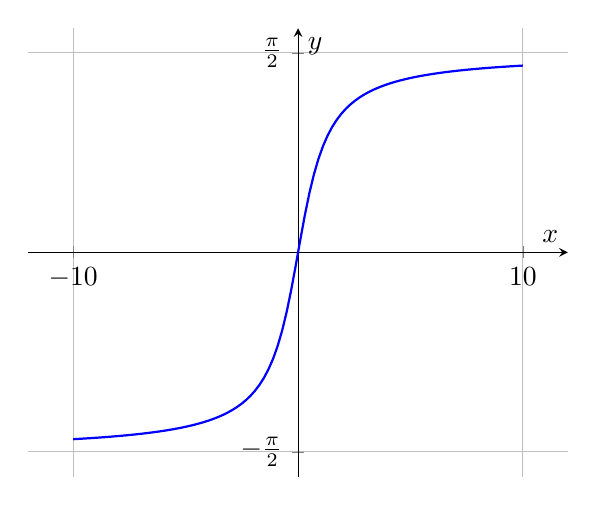
\begin{tikzpicture}
    \begin{axis}[
        domain=-10:10, % Setting a larger domain for atan to show its behavior
        samples=100,
        xlabel={$x$},
        ylabel={$y$},
        xtick={-10,0,10},
        ytick={-1.5708,0,1.5708}, % Using decimal approximations of -pi/2, 0, and pi/2 for tick positions
        yticklabel style={
            /pgf/number format/fixed,
            /pgf/number format/precision=5
        },
        yticklabels={$-\frac{\pi}{2}$, $0$, $\frac{\pi}{2}$},
        axis lines=center,
        enlargelimits=true,
        grid=major
    ]
    \addplot[blue, thick] {rad(atan(x))}; % Use rad() to ensure the result is in radians
    \end{axis}
  \end{tikzpicture}
  \end{minipage}
  \begin{minipage}[]{0.47\textwidth}
  \end{minipage}

  \pagebreak \bigbreak \noindent 
  \begin{minipage}[]{0.47\textwidth}
        \incfig{arcthing2}
  \end{minipage}
  \begin{minipage}[]{0.47\textwidth}
    \incfig{arcthing3}
  \end{minipage}
  \bigbreak \noindent 
\begin{figure}[ht]
    \centering
    \incfig{arcthing4}
    \label{fig:arcthing4}
\end{figure}


    \pagebreak \bigbreak \noindent
    \begin{center}
      \section{\Large{Calc 1}}
    \end{center}
    \line(1,0){490}
    \bigbreak \noindent \bigbreak \noindent 
    \subsection{Secant Lines}
    \begin{itemize}
      \item Secent lines on a graph is a line through the curve that touces at 2 places.
      \item To find the slope of the secent line:
        \begin{align*}
          m_{pq} = \frac{y_{2}-y_{1}}{x_{2}-x_{1}}\ rather,\ \frac{P_{y} - Q_{y}}{P_{x}-Q_{x}}
        .\end{align*}
    \end{itemize}
    \bigbreak \noindent 
    Secant line:
    \begin{figure}[ht]
        \centering
        \incfig{secline}
        \label{fig:secline}
    \end{figure}

    \bigbreak \noindent \bigbreak \noindent
    \subsection{Tangent Lines}
    \begin{itemize}
      \item Tangent lines on a graph is a line that touches the curve exactly one time.
      \item Achieve an aproximation of the slope of the tangent line by moving Q closer to the tangent line and finding the slope of the secent line, we write
        \begin{align*}
          \lim\limits_{Q \to P}{m_{PQ} = m}
        .\end{align*}
      \item To write the equation of the tangent line, use point slope form:
        \begin{align*}
          y- y_{1} = x(x-x_{1})
        .\end{align*}
    \end{itemize}


    \bigbreak \noindent \bigbreak \noindent 
    \subsection{The Velocity Problem}
    \begin{itemize}
      \item Average velocity is denoted by the slope of the secant line 
      \item Instantaneous velocity is denoted by the slope of the tangent line
    \end{itemize}

    \bigbreak \noindent \bigbreak \noindent 
    \subsection{The Limit of a Function}
    \begin{itemize}
      \item Consider the function:
        \begin{align*}
          f(x) = x^{2} + 2
        .\end{align*}
        \begin{itemize}
          \item If we want to investigate x=2, we can draw a table and examine what does the value of $f(x)$ approach as x approaches 2
        \end{itemize}
      \item So we say:
        \begin{align*}
          \lim\limits_{x \to a}{f(x) = L}
        .\end{align*}
    \end{itemize}

    \bigbreak \noindent \bigbreak \noindent 
    \subsection{One Sided Limits}
    \begin{itemize}
      \item Approaching from the left (left hand limit):
        \begin{align*}
          \lim\limits_{x \to a-}{f(x)}
        .\end{align*}
        \begin{itemize}
          \item Plug in a and evaluate
        \end{itemize}
      \item Approaching from the right (right hand limit):
        \begin{align*}
          \lim\limits_{x \to a+}{f(x)}
        .\end{align*}
        \begin{itemize}
          \item Plug in a and evaluate
        \end{itemize}
      \item Know that:
        \begin{align*}
          \lim\limits_{x \to a}{f(x) = l}\ \Leftrightarrow \lim\limits_{x \to a-}{f(x) = l}\ \wedge \lim\limits_{x \to a+}{f(x) = l}
        .\end{align*}
    \end{itemize}

    \bigbreak \noindent \bigbreak \noindent 
    \subsection{Trig function limits}
    \bigbreak \noindent 
    We have the formulas:
    \begin{align*}
      &\lim\limits_{\theta  \to 0}{\frac{\sin{\theta }}{\theta }} = 1 \quad \lim\limits_{\theta  \to 0}{\frac{\theta }{\sin{\theta}}} = 1 \\
      &\lim\limits_{\theta \to 0}{\frac{\cos{\theta } - 1}{\theta }} = 0 \quad \lim\limits_{\theta  \to 0}{\frac{1-\cos{\theta }}{\theta }} = 0
    .\end{align*}




    \bigbreak \noindent \bigbreak \noindent 
    \subsection{Infinite Limits}
      \bigbreak \noindent 
      Consider:
      \begin{figure}[ht]
          \centering
          \incfig{inf}
          \label{fig:inf}
      \end{figure}
      \bigbreak \noindent 
      We can see that:
      \begin{align*}
        \lim\limits_{x \to 0+}{f(x) = \infty}
      .\end{align*}
      \bigbreak \noindent 
      And:
      \begin{align*}
        \lim\limits_{x \to 0-}{f(x) = -\infty}
      .\end{align*}
      \bigbreak \noindent 
      Therefore we have determined that x=0 is a vertical asymptote, in general, we can safely say that f(x) has a vertical asymptote at a if any of the limits as $x \rightarrow a  = \infty\ or -\infty$ 
      \bigbreak \noindent
        What if we have a $\frac{Nonzero\ Constant}{Approaching\ Zero} $?
        \bigbreak \noindent 
          \begin{itemize}
            \item say we have the equation:
              \begin{align*}
                \lim\limits_{x \to 5-}{\frac{x+1}{x-5}}
              .\end{align*}
          \end{itemize}
          We can see that if we plug in 5, we get $\frac{6}{0}$, so since we have a $\frac{Nonzero\ Constant}{Approaching\ Zero}$, we know that our limit is either going to be $\infty\ or\ -\infty $, the way we determite the sign of infinity is as follows:
          \begin{enumerate}
            \item Plug in a number close to $a$ in whatever direction your limit is, the sign of the output will be the sign of infinity.
          \end{enumerate}
          \bigbreak \noindent \bigbreak \noindent
          \nt{If the limit does not specify a side, test with number close to $a$ in both directions, if the sign is not the same, the limit is DNE}


      \bigbreak \noindent \bigbreak \noindent 
      \subsection{Limit Laws}
      \begin{itemize}
        \item $\lim\limits_{x \to a}{f(x) + g(x)} = \lim\limits_{x \to a}{f(x)} + \lim\limits_{x \to a}{g(x)}$ \ \ \ \  \ \ \ \ \ \ \ \ \ \ \ \ \ \ \ \ \ \ \ \ \ \ \ \ \ \ \ \ \ \ \  \textbullet $\lim\limits_{x \to a}{f(x)- g(x)} = \lim\limits_{x \to a}{f(x)} - \lim\limits_{x \to a}{g(x)} $
        \item $\lim\limits_{x \to a}{cf(x)} = c \cdot \lim\limits_{x \to a}{f(x)} $ \ \ \ \ \ \ \ \ \ \ \ \ \ \ \ \ \ \ \ \ \ \ \ \ \ \ \ \ \ \ \ \ \ \ \ \ \ \ \ \ \ \ \ \ \ \ \ \ \ \ \ \ \ \  \textbullet $\lim\limits_{x \to a}{f(x)\cdot g(x)} = \lim\limits_{x \to a}{f(x) } \cdot \lim\limits_{x \to a}{g(x)} $
        \item $\lim\limits_{x \to a}{\frac{f(x)}{g(x)}} = \frac{\lim\limits_{x \to a}{f(x)}}{\lim\limits_{x \to a}{g(x)}},\ \ \text{if g(x) $\neq0$} $  \ \  \ \ \ \ \  \ \ \ \ \ \ \ \ \ \ \ \ \textbullet $\lim\limits_{x \to a}{\bigg(f(x)\bigg)^{n}}  = \bigg[\lim\limits_{x \to a}{f(x)}\bigg]^{n}$, where n is a positive integer
        \item $\lim\limits_{x \to a}{c} = c $  \ \ \ \ \ \ \ \ \ \ \ \ \ \ \ \ \ \ \ \ \ \ \ \  \ \ \ \ \ \ \ \ \ \ \ \ \ \ \ \ \ \ \ \ \ \ \ \ \ \ \ \  \ \ \ \ \  \ \ \ \ \ \ \    \  \ \ \ \ \ \ \  \ \ \textbullet $\lim\limits_{x \to a}{x} = a $
        \item $\lim\limits_{x \to a}{x^{n}} = a^{n}$, where n is a positive integer \ \ \ \ \ \  \ \ \ \ \ \ \  \ \ \ \ \ \ \ \ \  \ \ \textbullet $\lim\limits_{x \to a}{\sqrt[n]{x}} = \sqrt[n]{a} $, where n is a positive integer
        \item $\lim\limits_{x \to a}{\sqrt[n]{f(x)}} = \sqrt[n]{\lim\limits_{x \to a}{f(x)}} $, where n is a positive integer
      \end{itemize}

      \bigbreak \noindent \bigbreak \noindent 
      \subsection{Direct Substitution Property}
      \begin{itemize}
        \item You can plug in $a$ and evaluate, if a is not in the domain of $f(x)$, you can try factoring
      \end{itemize}

      \pagebreak \bigbreak \noindent
      \subsection{Continuity}
      \bigbreak \noindent \bigbreak \noindent
      For a function to have continuity $at a$, 3 things must be true:
      \begin{enumerate}
        \item f(x) is defined at $a$
        \item $\lim\limits_{x \to a}{f(x)}$ exists
        \item $\lim\limits_{x \to a}{f(x) = f(a)} $
      \end{enumerate}
      If no. 3 is true, the function is automatically continous at $a$

      \bigbreak \noindent \bigbreak \noindent 
      \subsection{One-Sided Continuity}
      \begin{itemize}
        \item Continuity from the right:
          \begin{align*}
            \lim\limits_{x \to a+}{f(x)=f(a)}
          .\end{align*}
        \item Continuity from the left:
          \begin{align*}
            \lim\limits_{x \to a-}{f(x)=f(a)}
          .\end{align*}
      \end{itemize}
      \bigbreak \noindent \bigbreak \noindent
      If $f$ and $g $ are continuous at $a $, then:
      \begin{itemize}
        \item $f+g $
        \item $f-g $
        \item $fg $
        \item $\frac{f}{g} $
        \item $cf $
      \end{itemize}
      \bigbreak \noindent 
      Are all continuous at $a $
      \bigbreak \noindent \bigbreak \noindent
      Also:
      \begin{itemize}
        \item Any polynomial is continous on its domain ($ \mathbb{R} $)
        \item Any rational function is continous on its domain
      \end{itemize}
      \bigbreak \noindent \bigbreak \noindent
      \nt{If $ \lim\limits_{x \to a}{f(x)} $ exists, Then you don't need to worry about which side the continuity is coming from}

      \pagebreak \bigbreak \noindent
      \subsection{Discontinuitys}
      \begin{figure}[h]
          \centering
          \incfig{removeable}
          \incfig{removebale2}
          \label{fig:removeable}
      \end{figure}

      \begin{figure}[h]
          \centering
          \incfig{infinity}
          \incfig{jump}
          \label{fig:infinity}
      \end{figure}

      \bigbreak \noindent \bigbreak \noindent
      \subsection{Finding where a function is Discontinuous without the graph of f}
      \begin{itemize}
        \item Zeros of a rational function
        \item if $ \lim\limits_{x \to a}{f(x) \neq f(a)} $
        \item Piecewise functions, examine values of x where the domain flips to see if the limit is DNE
      \end{itemize}

      \bigbreak \noindent \bigbreak \noindent 
      \subsection{Intermediate Value Theorem}
      \bigbreak \noindent \bigbreak \noindent
      Suppose f is continuous on [a,b], Let N be any number between f(a) and f(b), where $f(a) \neq f(b)$, then:
      \begin{align*}
        \exists\ c \in (a,b)\ |\ f(c) = N
      .\end{align*}

      

      \pagebreak \bigbreak \noindent
      \subsection{Evaluating limits at infinity (horizontal asymptotes)}
      \bigbreak \noindent 
      We have a horizontal Asymptote if:
      \begin{align*}
        \lim\limits_{x \to \infty}{f(x) = L }\\ 
        Or:
        \lim\limits_{x \to -\infty}{f(x) = L}
      .\end{align*} 
        \begin{itemize}
          \item Recall: If the degree of the numerator is higher than the degree of the denominator, the H.A is automatically y = 0
          \item For rational Functions: divide every term in the numerator and denominator by the highest degree in the denominator, then take the limit of each new term.
          \item Radical types like:
          \begin{align*}
            \lim_{x \to \infty}{\sqrt{x^{2}+4x}-x}
          .\end{align*}
          \begin{enumerate}
            \item Conjugate (Multiply both numerator and denominator)
            \item pull out the 4
            \item divide numerate by x
            \item divide insider radical by $x^{2}$ and +x by x
            \item evaluate
          \end{enumerate}
          \item Example:
          \begin{align*}
            \lim\limits_{x \to -\infty}{\frac{\sqrt{9x^{6}-x}}{x^{3}+1}}
          .\end{align*}
          Since $\sqrt{x^{6}} = x^{3}$, we need to put absolute value bars and write as piecewise:
             \begin{equation}
              \abs{x^{3}}=
                  \begin{cases}
                      x^{3} & \text{if }  x \geq 0 \\
                       -(x^{3})& \text{if } x < 0 
                  \end{cases}
              \end{equation}
          And since our limit is going to negative infinity, we use $-x^{3} $
          \begin{align*}
            \lim\limits_{x \to -\infty}{\frac{-\sqrt{\frac{9x^{6}-x}{x^{6}}}}{\frac{x^{3}+1}{x^{3}}}} \\
            = \frac{-\sqrt{9-\frac{1}{x^{5}}}}{1+\frac{1}{x^{3}}} \\
            = \frac{-\sqrt{9-0}}{1+0} \\
            = -3
          .\end{align*}
        \end{itemize}
    \begin{itemize}
      \item Limits at infinty of Polynomials
        \begin{itemize}
          \item Say we have:
            \begin{align*}
              \lim_{x \to -\infty}{5+2x-x^{3}}
            .\end{align*}
          \item In this case, we can forget about the insignificant terms and only focus on $-x^{3}$, which means.
            \begin{align*}
              \lim_{x \to -\infty}{-x^{3}} = -(-\infty)^{3} \\
              = \infty
            .\end{align*}
        \end{itemize}
    \end{itemize}
    \begin{itemize}
      \item Find equation of horizontal Asymptote by looking at limtit at infinity
        \begin{itemize}
          \item If the limit as x approaches infinity is a constant, then the equation of the H.A is y = L, where L is the constant
          \item if the limit as x approches infinity of a rational function is bottom heavy then the equation of the H.A is y = 0 
        \end{itemize}
    \end{itemize}

    \bigbreak \noindent \bigbreak \noindent 
    \subsection{Derivatives and rates of change (Definitions)}
    \begin{itemize}
      \item Slope of Secant Line:
        \begin{align*}
          m_{PQ} = \frac{f(x)- f(a)}{x-a} \\
          or: 
          \frac{f(a+h)- f(a)}{h}
        .\end{align*}
      \item Slope of Tangent Line:
        \begin{align*}
          m_{tan} = \lim\limits_{x \to a}{\frac{f(x)- f(a)}{x-a}} \\
          or: 
          \lim\limits_{h \to 0}{\frac{f(a+h)- f(a)}{h}}
        .\end{align*}
      \item Average Velocity:
        \begin{align*}
          v_{ave} = \frac{f(x)- f(x)}{x-a}
        .\end{align*}
      \item Instantaneous Velocity:
        \begin{align*}
          v_{inst} = \lim\limits_{x \to a}{\frac{f(x)- f(a)}{x-a}} \\
          or: 
          \lim\limits_{h \to 0}{\frac{f(a+h)- f(a)}{h}}
        .\end{align*}
      \item Speed:
        \begin{align*}
          Speed\ = \abs{Velocity}
        .\end{align*}
      \item Derivatives Definition:
        \begin{align*}
          f^{\prime}(x) = \lim\limits_{x \to a}{\frac{f(x)-f(a)}{x-a}} \\
          Or:
          f^{\prime}(x) = \lim\limits_{h \to 0}{\frac{f(x+h)-f(x)}{h}}
        .\end{align*}
      \item Know that:
    \begin{align*}
      s(t) = postition\ function \\
      v(t) = s^{\prime}(t) = velocity\ function \\
      a(t) = v^{\prime}(t) = acceleration\ function
    .\end{align*}
    \end{itemize}
    \bigbreak \noindent \bigbreak \noindent 
    \nt{If f(x) is differentiable at $a$, then it is continous at $a$, the converse is not true}

    \pagebreak \bigbreak \noindent
    \subsection{Differential Rule}
    \bigbreak \noindent \bigbreak \noindent 
    Properties of Derivatives:
    \begin{itemize}
      \item $\frac{d}{dx}c  = 0$
      \item $\frac{d}{dx}x  = 1$
      \item $ \frac{d}{dx}(x^n) = n \cdot x^{n-1} \rightarrow$ \text{\textbf{\textit{Power Rule}}}
      \item $ \frac{d}{dx}[c \cdot f(x)] = c \cdot \frac{d}{dx}[f(x)]$
      \item $ \frac{d}{dx}[f(x) \pm g(x)] = \frac{d}{dx}f(x)\pm \frac{d}{dx}g(x)$
    \end{itemize}


    \bigbreak \noindent \bigbreak \noindent 
    \subsection{Derivatives of common functions}
    \bigbreak \noindent 
    Exponential Functions:
    \begin{itemize}
      \item $\frac{d}{dx}e^{x} = e^{x} \cdot \frac{d}{dx}x$
      \item $\frac{d}{dx}a^{x} = a^{x} \cdot \ln{a} \cdot \frac{d}{dx}x$
      \item $\frac{d}{dx}\ln{x}  = \frac{1}{x} \cdot \frac{d}{dx}x$
      \item $\frac{d}{dx}\log_a{x} = \frac{1}{x \cdot \ln{a}} \cdot \frac{d}{dx}x$
    \end{itemize}
    \bigbreak \noindent \bigbreak \noindent
    Trig Functions:
    \begin{itemize}
      \item $\frac{d}{dx}\sin{x}  = \cos{x}$
      \item $\frac{d}{dx}\cos{x}  = -\sin{x}$
      \item $\frac{d}{dx}\tan{x} = \sec^{2}{x} $
      \item $\frac{d}{dx}\csc{x} = -\csc{x}\cot{x} $
      \item $\frac{d}{dx}\sec{x} = \sec{x}\tan{x} $
      \item $\frac{d}{dx}\cot{x} = -\csc^{2}{x} $
    \end{itemize}
    \bigbreak \noindent \bigbreak \noindent
    Inverse Trig:
    \begin{itemize}
      \item $\frac{d}{dx}$arcsin(x) = $\frac{1}{\sqrt{1-x^{2}}}$
      \item $\frac{d}{dx}$arccos(x) = -$\frac{1}{\sqrt{1-x^{2}}}$
      \item $\frac{d}{dx}$arctan(x) = $\frac{1}{x^{2}+1}$
      \item $\frac{d}{dx}$arccsc(x) = $-\frac{1}{x\sqrt{x^{2}-1}}$
      \item $\frac{d}{dx}$arcsec(x) = $-\frac{1}{x\sqrt{x^{2}-1}}$
      \item $\frac{d}{dx}$arccot(x) = $-\frac{1}{x^{2}+1}$
    \end{itemize}

    \pagebreak \bigbreak \noindent
    \bigbreak \noindent \bigbreak \noindent
    Hyperbolic Trig
    \begin{itemize}
      \item $\frac{d}{dx}\sinh{x}  = \cosh{x}$
      \item $\frac{d}{dx}\cosh{x} = \sinh{x}$
      \item $\frac{d}{dx}\tan{x} = sech^{2}x$
      \item $\frac{d}{dx}csch{x} = -csch{x}cothx$
      \item $\frac{d}{dx}sech{x} = -sechxtanhx$
      \item $\frac{d}{dx}coth{x} = -csc^{2}x$
    \end{itemize}

    \bigbreak \noindent \bigbreak \noindent 
    \subsection{Normal Line}
    \begin{itemize}
      \item The normal line is Perpendicular to the tangent line at the point of tangency, which means:
        \begin{align*}
          m_{tan} \cdot m_{normal} = -1
        .\end{align*}
        \begin{itemize}
          \item In other words, they are opposite reciprocals so flip and change sign
        \end{itemize}
    \end{itemize}

    \bigbreak \noindent \bigbreak \noindent 
    \subsection{Find equation of tangent and normal line}
    \bigbreak \noindent \bigbreak \noindent
    Say we have the equation and point:
    \begin{align*}
      y=x^4 + 8e^x\ \text{at the point (0,8).}
    .\end{align*}
    \begin{enumerate}
      \item Find derivative
      \item Plug in x into derivative function
      \item Flip $m_{tan}$ and change the sign to find $m_{normal} $
      \item Use point slope form to find equations
    \end{enumerate}


    \bigbreak \noindent \bigbreak \noindent 
    \subsection{Product and Quotient Rule}
    \begin{itemize}
      \item Product rule:
        \begin{align*}
          \frac{d}{dx}[f(x) \cdot g(x)] = f(x) \frac{d}{dx}[g(x)] + g(x) \frac{d}{dx}[f(x)]
        .\end{align*}
      \item Quotient Rule:
        \begin{align*}
          \frac{d}{dx}\bigg[ \frac{f(x)}{g(x)}\bigg] = \frac{g(x) \frac{d}{dx}[f(x)] - f(x) \frac{d}{dx}[g(x)]}{[g(x)]^2}
        .\end{align*}
    \end{itemize}

    \bigbreak \noindent \bigbreak \noindent 
    \subsection{Chain Rule}
    \begin{itemize}
      \item Know the chain rule:
        \begin{itemize}
          \item If:
        \begin{align*}
          F(x) = f(g(x))
        .\end{align*}
        \item Then:
        \begin{align*}
          F^{\prime}(x) = f^{\prime}(g(x)) \cdot g^{\prime}(x)
        .\end{align*}
        \end{itemize}
    \end{itemize}

    \pagebreak \bigbreak \noindent
    \subsection{Implicit Differentation}
    \bigbreak \noindent 
    Procedure:
    \begin{enumerate}
      \item Differentiate
      \item Leave $\frac{dy}{dx}$ next to terms of y that you differentiate
      \item solve for $\frac{dy}{dx}$
    \end{enumerate}
    \bigbreak \noindent \bigbreak \noindent 
    Example:
    \begin{align*}
      2x^{3}  +x^{2}y-xy^{3} =2 \\
      =     6x^{2} + (x^{2} \cdot 1\cdot \frac{dy}{dx} + 2x \cdot y) - (x \cdot 3y^{2} \cdot \frac{dy}{dx} +y^{3}\cdot 1) =  0 \\
         =  6x^{2} + x^{2}\frac{dy}{dx}+2xy - 3xy^{2}\frac{dy}{dx}- y^{3} = 0 \\
         =    x^{2}\frac{dy}{dx}-3xy^{2}\frac{dy}{dx} = y^{3}-6x^{2}-2xy \\
         =     \frac{dy}{dx}(x^{2}-3xy^{2}) = y^{3} - 6x^{2} - 2xy \\
         =    \frac{dy}{dx} = \frac{y^{3}-6x^{2}-2xy}{x^{2}-3xy^{2}} 
    .\end{align*}

    \bigbreak \noindent \bigbreak \noindent 
    \subsection{Logarithmic Differentation}
    \bigbreak \noindent 
    If you have a problem that uses chain rule, product rule, quotient rule, all together. It's best to use this Logarithmic definition
    \bigbreak \noindent 
    Or if you have an equation with a variable in the base, and as the exponent, like:
    \begin{align*}
      y  = (\cos{5x})^{x}
    .\end{align*}
    \bigbreak \noindent \bigbreak \noindent 
    Procedure:
    \begin{enumerate}
      \item Take ln of both sides
      \item Differentiate implicitly with respect to x
      \item solve for $y^{\prime} $
    \end{enumerate}
    Example:
    \begin{align*}
      y = \sqrt[4]{\frac{x^{2}+1}{x^{2}-1}} \\
      \ln{y} = \ln{\bigg({\frac{x^{2}+1}{x^{2}-1}}\bigg)^{\frac{1}{4}}} \\
      \frac{1}{y}\frac{dy}{dx} = \frac{1}{4}\ln{\bigg({\frac{x^{2}+1}{x^{2}-1}}\bigg)} \\
      \frac{1}{y}\frac{dy}{dx} = \frac{1}{4}\ln{(x^{2}+1)} - \frac{1}{4}\ln{(x^{2}-1)} \\
      \frac{1}{y}\frac{dy}{dx} = \frac{1}{4}\bigg(\frac{1}{x^{2}+1} \cdot 2x\bigg) - \frac{1}{4}\bigg(\frac{1}{x^{2}-1} \cdot 2x\bigg) \\
      \frac{1}{y}\frac{dy}{dx} = \frac{x}{2(x^{2}+1)} - \frac{x}{2(x^{2} -1)} \\
      \frac{1}{y}\cdot \frac{dy}{dx} = \frac{x}{2(x^{2}+1)} \cdot \frac{x^{2}-1}{x^{2} -1} - \frac{x}{2(x^{2} -1)} \cdot \frac{x^{2}+1}{x^{2}+1}\\
      \frac{1}{y}\cdot \frac{dy}{dx} = \frac{x(x^{2}-1)}{2(x^{2}+1)(x^{2}-1)}  - \frac{x(x^{2}+1)}{2(x^{2} -1)(x^{2}+1)} \\
      \frac{1}{y}\cdot \frac{dy}{dx} = \frac{x^{3}-x}{2(x^{2}+1)(x^{2}-1)}  - \frac{x^{3}+x}{2(x^{2} -1)(x^{2}+1)} \\
      \frac{1}{y}\cdot \frac{dy}{dx} = \frac{x^{3}-x-(x^{3}+x)}{2(x^{2}+1)(x^{2}-1)}   \\
      \frac{1}{y}\cdot \frac{dy}{dx} = \frac{x^{3}-x-x^{3}-x}{2(x^{4}-1)}   \\
      \frac{1}{y}\cdot \frac{dy}{dx} = \frac{-2x}{2(x^{4}-1)}   \\
      \frac{1}{y}\cdot \frac{dy}{dx} = \frac{-x}{x^{4}-1}   \\
    .\end{align*}
    Solve for $\frac{dy}{dx}$ and plug in original equation for y:
    \begin{align*}
      \frac{dy}{dx} = \frac{-x}{x^{4}-1} \cdot y \\
      \frac{dy}{dx} = \frac{-x}{x^{4}-1} \cdot \sqrt[4]{\frac{x^{2}+1}{x^{2}-1}}
    .\end{align*}

    \pagebreak \bigbreak \noindent
    \subsection{Rates of Change in the natural and social sciences}
    \bigbreak \noindent 
    Velocity:
    \begin{itemize}
      \item Velocity is derivative of position function
      \item A particle is at rest when $v(t) = 0 $
      \item a particle reaches its maximum height when v(t) = 0
      \item A particle is moving in the positive direction when $v(t) > 0 $
      \item A particle is moving in the negative direction when $v(t) < 0 $
    \end{itemize}
    \bigbreak \noindent \bigbreak \noindent 
    Acceleration:
    \begin{itemize}
      \item A particle is speeding up when v(t) and a(t) have the same signs
      \item A particle is slowing down when v(t) and a(t) have opposite signs
    \end{itemize}

    \bigbreak \noindent \bigbreak \noindent 
    \subsection{Exponential Growth and Decay}
    \bigbreak \noindent \bigbreak \noindent
    Formula:
    \begin{align*}
      y = Ce^{kt} \\
      y = Population \\
      C =\ intitial\ Population \\
      k = \frac{Growth\ Rate}{Population} \\
      t = time
    .\end{align*}

    \bigbreak \noindent \bigbreak \noindent
    For example, if a bacterial culture starts with 4000 bacteria and triples every half hour.:

    \bigbreak \noindent \bigbreak \noindent
    So:
    \begin{align*}
      y = 4000e^{kt},\ \ \ (\frac{1}{2}, 12000)
    .\end{align*}
    \bigbreak \noindent \bigbreak \noindent
    Then we can solve for k:
    \begin{align*}
      12000 = 4000e^{k(\frac{1}{2})} \\
      3 = e^{\frac{k}{2}} \\
      \ln{3} = \frac{k}{2} \\
      k = 2\ln{3}
    .\end{align*}
    \bigbreak \noindent 
    So we have:
    \begin{align*}
      y = 4000e^{2\ln{3}(t)}
    .\end{align*}

    \pagebreak \bigbreak \noindent
    \subsection{Newton's Law of Cooling}
    \bigbreak \noindent \bigbreak \noindent
    Newton's Law of cooling states:
    \begin{align*}
      T(t) = t_{s} + Ce^{kt} \\
      T(t) =\ \text{Temperature at time $t$} \\
      t_{s} =\ \text{Temperature of surrounding area} \\
      C = t_{0} - t_{s}
    .\end{align*}

    \bigbreak \noindent \bigbreak \noindent
    Say we have a freshly brewed cup of coffee has a temperature of $95^{\circ}C$ in a $20^{\circ}C$ room, five minutes
    later, its temerature is $88^{\circ}C$

    \bigbreak \noindent \bigbreak \noindent
    Then
    \begin{align*}
      T(t) = 88 \\
      t_{s} = 20 \\
      C = t_{0} - t_{s} = 95 - 20  = 75 \\
      t = 5
    .\end{align*}
    \bigbreak \noindent \bigbreak \noindent
    So our equation would be.
    \begin{align*}
      88 = 20 + 75e^{k(5)} \\
      68 = 75e^{5k} \\
      \frac{68}{75} = e^{5k} \\
      \ln{\frac{68}{75}} = 5k \\
      k = \frac{\ln{\frac{68}{75}}}{5} \\
      \approx  - 0.0196
    .\end{align*}

    \pagebreak \bigbreak \noindent
    \subsection{Related Rates}
      \bigbreak \noindent 
    Many things change with item. Our goal is to find the rate at which some 
    quantity is changing by relating it to other quantities whose rates of 
    change are given or more easily measured 
    \bigbreak \noindent 
    \textbf{Strategy}
    \begin{enumerate}
      \item Read the problem carefully
      \item Draw a diagram whenever possible
      \item Introduce notation
      \item Express rates in terms of derivatives
      \item Write an equation 
      \item Differentiate both sides with repect to $t$ using Implicit Differentiation/Chain Rule
      \item Solve for the unknown rate
    \end{enumerate}

    \bigbreak \noindent \bigbreak \noindent
    Say the length of a rectangle is increasing at a rate of 8 cm/s and it’s width is increasing at a rate
of 3 cm/s. When the length is 20cm and the width is 10cm, how fast is the area increasing?

    \bigbreak \noindent \bigbreak \noindent
    So our givens:
    \begin{align*}
      \frac{dl}{dt} = 8 \\
      \frac{dw}{dt} = 3 \\
      l = 20 \\
      w =10
    .\end{align*}

    \bigbreak \noindent 
    We want:
    \begin{align*}
      \frac{dA}{dt}
    .\end{align*}

    \bigbreak \noindent \bigbreak \noindent
    And we know that:
    \begin{align*}
      A = l \cdot w
    .\end{align*}

    \bigbreak \noindent 
    So if we derive the area formula with Implicit differentation, and using the product rule, we get:
    \begin{align*}
      \frac{dA}{dt} = l \cdot \frac{dw}{dt} + w \cdot \frac{dl}{dt}
    .\end{align*}

    \bigbreak \noindent 
    From here we can plug in our givens:
    \begin{align*}
      \frac{dA}{dt} = 20(3) + 10(8) \\
      = 60 +80 \\
      = 140cm^{2}/s
    .\end{align*}

    \pagebreak \bigbreak \noindent
    \subsection{Linear Approximation}
    \bigbreak \noindent \bigbreak \noindent
    Formula:
    \begin{align*}
      f(x) \approx  L(x) =f(a) + f^{\prime}(a)(x-a)
    .\end{align*}
    \bigbreak \noindent \bigbreak \noindent
    \nt{Finding the linearization of a function is the same thing as "find the equation of the tangent line to the curve"}
    \bigbreak \noindent \bigbreak \noindent
    Procedure, 
    \begin{enumerate}
      \item find derivative of function
      \item plug in a to get $m_{tan} $
      \item Get point by plugging in a to $f(x)$
      \item plug everything into formula $L(x) = f(a)- f^{\prime}(a)(x-a) $
    \end{enumerate}
    \bigbreak \noindent \bigbreak \noindent
    If asked to use linear aproximation formula to approximate values, then:
    \begin{enumerate}
      \item set original function equal to value
      \item solve for x
      \item plug in for x in linear approximation formula
    \end{enumerate}

    \bigbreak \noindent \bigbreak \noindent 
    \subsection{Differentials}
    \bigbreak \noindent 
    Formula:
    \begin{align*}
      dy = f^{\prime}(x)dx \\
      \Delta x = dx \\
      \Delta y = (f(x+\Delta x) -f(x))
    .\end{align*}
    \bigbreak \noindent 
    \nt{$\Delta y $, can sometimes be difficult to find so we can use $dy \approx \Delta y $}


    \pagebreak \bigbreak \noindent
    \subsection{Maximum and Minimum Values}
    \bigbreak \noindent 
    \begin{itemize}
      \item A function $f$ has an absolute maximum at  $c$ if $f(c) \geq f(x)$ for all $x \in$ Domain of $f$
      \item A function $f$ has an absolute minimum at $k$ if  $f(c) \leq f(x)$ for all  $x \in$ Domain of  $f$
      \item A function $f$ has a local maximum at  $b$ if  $f(b) \geq f(x)$ when  $x$ is near  $b$
      \item A function $f$ has a local minimum at  $m$ if  $f(m) \leq f(x)$ when  $x$ is near  $m$
      \item endpoints are not considered local min max
    \end{itemize}
    \bigbreak \noindent \bigbreak \noindent
    Cosider This Graph
    \begin{figure}[ht]
        \centering
        \incfig{graph123}
        \label{fig:graph123}
    \end{figure}
    \bigbreak \noindent \bigbreak \noindent
    Note that the textbook denotes $f(1)=3 $ as a local minimum.

    \bigbreak \noindent \bigbreak \noindent 
    \subsection{Extreme Value Theorem}
    \begin{itemize}
      \item If $f$ is continuous on a closed interval [a,b], then $f$ attains an
      obsulute maximum value $f(c)$ and an absolute minimum value $f(d)$ where $c,d \in [a,b]$
    \end{itemize}

    \bigbreak \noindent \bigbreak \noindent 
    \subsection{Fermat's Theorem}
    \begin{itemize}
      \item If $f$ has a local minimum or maximum at $c$, and if $f^{\prime}(c)$ exists, 
      then $f^{\prime}(c)=0$
    \end{itemize}

    \bigbreak \noindent \bigbreak \noindent 
    \subsection{Critical Number}
    \begin{itemize}
      \item $c$ in the domain of $f(x)$ is a critical number if $f^{\prime}(c)=0$ or if $f^{\prime}(c)$ does not exist. \\
      Note: If $f$ has a local max or min at $c$, then $c$ is a critical number of $f$ 
      \item Critical number has to obey restriction
    \end{itemize}

    \bigbreak \noindent \bigbreak \noindent 
    \subsection{How to find the absolute maximum and minimum values of a continuous function f on a closed interval [a,b]}
      \begin{enumerate}
      \item Find critical values of f in (a,b)
      \item Find $f(a)$ and $f(b)$
      \item Absolute Max: largest from 1.) and 2.) 
      \item Absolute Min: smallest from 1.) and 2.)
    \end{enumerate}

    \bigbreak \noindent \bigbreak \noindent 
      \begin{large}
        \noindent \textbf{Rolle's Theorem:}
      \end{large}
     \bigbreak \noindent 
     If f(x) satisfies the following:
     \begin{enumerate}
       \item continuous on [a,b]
        \item differentiable on (a,b)
        \item f(a) = f(b)
     \end{enumerate}
     \smallbreak \noindent
     Then:
     \begin{align*}
       \{\exists\ c \in (a,b)\ |\ f^{\prime}(c) = 0\}
     .\end{align*}
     % Then there is a $c \in (a,b)$ such that $f^{\prime}(c) = 0$ 

     \bigbreak \noindent 
     Notes:
     \begin{itemize}
       \item If rolle's theorem can be applied, just set $f^{\prime}(x) = 0$ to find c, remember you are finding all c in the \textbf{\textit{\underline{open interval}}}, so if c does not obey this interval, it is not a solution
     \end{itemize}


     \bigbreak \noindent \bigbreak \noindent 
     \subsection{The Mean Value Theorem}
      \bigbreak \noindent 
     if f(x) satisfies the following:
     \begin{enumerate}
       \item continuous on [a,b]
        \item differentiable on (a,b)
     \end{enumerate}
     \smallbreak \noindent
     Then:
     \begin{align*}
       \bigg\{\exists\ c \in (a,b)\ |\ f^{\prime}(c) = \frac{f(b)- f(a)}{b-a}\bigg\}
     .\end{align*}
     % then there is a number $c \in (a,b)$ such that
     % \begin{align*}
     %   f^{\prime}(c) = \frac{f(b) - f(a)}{b -a}
     % .\end{align*}
     \bigbreak \noindent 
     In other words,
     \begin{align*}
       m_{tan} = m_{sec}
     .\end{align*}
     \bigbreak \noindent 
     Then after you solve for $f^{\prime}(c)$, set $f^{\prime}(x)$ equal to this value. This is how you compute c.
     \bigbreak \noindent \bigbreak \noindent
     Notes:
     \begin{itemize}
       \item If rational function, find where function is undefined, if that number is not an element of the interval, then it is continous on the closed interval
        \item If $f^{\prime}(x)$ is defined on the open interval, then it is differentiable on the open interval
        \item use the theorem, then set $f^{\prime}(c) = c$
     \end{itemize}

     \bigbreak \noindent 
     What if you just have a graph?
     \begin{enumerate}
       \item Draw a secant line through a and b
        \item Draw a tangent line such that the slopes are the same (they are parallel)
     \end{enumerate}

     \bigbreak \noindent \bigbreak \noindent 
     \subsection{First Derivative Test}
     \begin{itemize}
         \item  If $f^{\prime}(x)$ changes from + to - at $c$, then $f(x)$ has a local maximum at c.
        \item If $f^{\prime}(x)$ changes from - to + at $c$, then $f(x)$ has a local minimumc.
     \end{itemize}

     \bigbreak \noindent \bigbreak \noindent 
     \subsection{Second Derivative Test}
      \begin{itemize}
       \item f(x) has a local minimum at c if $f^{\prime}(c)=0$ and $f^{\prime\prime}(c) > 0$ 
       \item f(x) has a local maximum at c if $f^{\prime}(c)=0$ and $f^{\prime\prime}(c) < 0$ 
     \end{itemize}


     \bigbreak \noindent \bigbreak \noindent 
     \subsection{Domain}
    \begin{itemize}
      \item Polynomial: $ \mathbb{R} $
      \item rational: Where denominator = 0 
      \item Radical: Set denominator $\geq 0$, if needed, make a number line and test points to see where its positive.
    \end{itemize}

    \bigbreak \noindent \bigbreak \noindent 
    \subsection{Intercepts}
    \begin{itemize}
      \item x-ints: set function equal to zero and solve, if the function is rational, only set the numerator equal to zero
      \item y-ints: plug in zero for x and solve
    \end{itemize}

    \bigbreak \noindent \bigbreak \noindent 
    \subsection{Asymptotes}
    \begin{itemize}
      \item Horizontal Asymptote, find the limit of the function as x approaches infinity and -infinty, see limits at infinity for more info on rational functions
      \item vertical Asymptoteo, only for rational functions, it is the zeros of the function
      \item Slant (oblique), if numerater degree is one higher than denominator, use long division to find equation of slant Asymptote
    \end{itemize}
    \begin{align*}
      \frac{-8x^{4}+8x^{3}+4}{2x^{3}-x}
    .\end{align*}
    \begin{align*}
      2x^{3}+0x^{2}-x \overline{)-8x^{4}+8x^{3}+4}
    .\end{align*}
    \bigbreak \noindent 
    \textit{And:}
    \begin{align*}
      \frac{x^{2}+4}{x+4}
    .\end{align*}
    \begin{align*}
      x+4 \overline{)x^{2}+0x+4}
    .\end{align*}


    \bigbreak \noindent \bigbreak \noindent 
    \subsection{Symmetric}
    \begin{itemize}
      \item Even if (symmetric with respect to y axis)
        \begin{itemize}
          \item $f(-x) = f(x) $
        \end{itemize}
      \item Odd if (symmetric with respect to origin)
        \begin{itemize}
          \item $f(-x) = -f(x)$
        \end{itemize}
    \end{itemize}

    \bigbreak \noindent \bigbreak \noindent 
    \subsection{Increasing/Decreasing (Numberline with Domain (not as critical values but still test))}
    \begin{itemize}
      \item Find derivative
      \item set numerator equal to 0 to find critical values (make sure they are in the domain.)
      \item Make number line and test with $f^{\prime}(x)$, ontop of the critical values, use the values are found in domain
        \begin{itemize}
          \item ex.
            \begin{align*}
              (-\infty, -4]\cup [0,\infty]
            .\end{align*}
          \item use -4 and 0 on number line
        \end{itemize}
    \end{itemize}
    \bigbreak \noindent 
    Note: no brackets on intervals of increase/decrease
    \bigbreak \noindent \bigbreak \noindent 
    \begin{large}
      \textbf{Local Min/Max}
    \end{large}
    \begin{itemize}
      \item First derivative test: 
        \begin{itemize}
          \item If $f^{\prime}(x)$ switches from positive to negative, you have a local max at f(c)
          \item If $f^{\prime}(x)$ switches from negative to positive, you have a local min at f(c)
        \end{itemize}
      \item Second Derivative test: 
        \begin{itemize}
          \item If $f^{\prime\prime}(c) < 0$, you have a local max at $f(c)$
          \item If $f^{\prime\prime}(c) > 0$, you have a local min at $f(c)$
        \end{itemize}
    \end{itemize}


    \bigbreak \noindent \bigbreak \noindent 
    \subsection{Abs Max and Min}
      \begin{enumerate}
        \item find $f^{\prime}(x)$
        \item find critical values, plug into $f(x)$
        \item find $f(a)\ and\ f(b)$ from (a,b)
        \item Abs max: largest form top steps
        \item Abs min: smallest form top steps
      \end{enumerate}

    \bigbreak \noindent \bigbreak \noindent 
    \subsection{Concave Up/Down and inflection points}
    \begin{enumerate}
      \item Find $f^{\prime\prime}(x)$
      \item Find inflection points (Critical Values)
      \item Test inflection points on a number line
      \item If concavity changes at critical value, then plug in critical value to $f(x)$ to find inflection points
    \end{enumerate}
    \bigbreak \noindent 
    Note: If no $c \in D$, but domain is say $(-\infty, 15]$, use 15 on number line, but 15 cannot be an inflection point or numbers after used to test concavity
    \bigbreak \noindent 
    Find inflection points of $f(x)$, $f^{\prime}(x)$, and $f^{\prime\prime}(x)$, given the graph of $f(x)$
    \begin{itemize}
      \item $f(x)$: find inflection points by locating where on the graph does it switch concavity. (x values)
      \item $f^{\prime}(x)$: find inflection points by locating local min/maxs. (x values)
      \item $f^{\prime\prime}(x)$: Find inflection points by locating where it switches from positive to negative
    \end{itemize}
    \bigbreak \noindent 
    Consider the graph of f(x):
    \begin{figure}[ht]
        \centering
        \incfig{cosdire}
        \label{fig:cosdire}
    \end{figure}
    \bigbreak \noindent 
    \begin{align*}
      CU:\ (0,2) \\
      CD:\ (2,4)\cup (4,6) \\
      IP:\ (2,3)
    .\end{align*}
    \bigbreak \noindent \bigbreak \noindent
    \nt{Write inflection points as an ordered pair}
    \bigbreak \noindent \bigbreak \noindent 

    \pagebreak \bigbreak \noindent
    \subsection{ L'Hospital's Rule}
    \bigbreak \noindent 
    Main Concept:
    \begin{align*}
      \lim_{x \to a}{\frac{f(x)}{g(x)}} = \lim_{x \to a}{\frac{f^{\prime}(x)}{g^{\prime}(x)}}
    .\end{align*}
    \begin{itemize}
      \item Important concepts
        \begin{itemize}
          \item Review limits at infinity
          \item Any number other than zero or 1 to the power of negative infinity is 0
          \item Any number other than zero or 1 to the power of infinity is infinity
          \item The natural log of a negative number is undefined, therefore the limit as x approaches negative infinity of $\ln{x}$ is hence undefined
          \item Same with log
          \item Any contant over infinity approaches 0
        \end{itemize}
    \end{itemize}
    \begin{itemize}
      \item Types of indeterminate forms we do want
        \begin{itemize}
          \item $\frac{0}{0} $
          \item $\frac{\infty}{\infty} $
        \end{itemize}
    \end{itemize}
    \begin{itemize}
      \item Types of indeterminate forms we don't want:
        \begin{itemize}
          \item $0 \cdot \infty$
          \item $\infty - \infty $
          \item $0^{0} $
          \item $\infty^0 $
          \item $1^{\infty} $
        \end{itemize}
    \end{itemize}
    \begin{itemize}
      \item type $\infty-\infty$
        \begin{itemize}
          \item Change to the type we want by:
            \begin{enumerate}
              \item Common Denominators
              \item rationalizing
              \item factoring
            \end{enumerate}
        \end{itemize}
    \end{itemize}
    \begin{itemize}
      \item Types $0^{0}$, $\infty^{0}$, $1^{\infty} $
        \begin{itemize}
          \item Change to the type we want by:
            \begin{enumerate}
              \item taking natural log of function or writing as exponential
            \end{enumerate}
        \end{itemize}
    \end{itemize}

    \bigbreak \noindent \bigbreak \noindent 
    \nt{If you use natural log method, you must write final answer as $e^{ \lim_{x \to \infty}{\ln{y}}}$}


    \pagebreak \bigbreak \noindent
    \subsection{Curve Sketching}
    \begin{itemize}
      \item Find A-G and sketch graph
        \begin{itemize}
          \item A: Domain
          \item B: Intercepts
          \item C: Asymptotes
          \item D: Symmetry
          \item E: Local min/max
          \item F: Increasing / decreasing
          \item G: Concavity / Inflection Points
        \end{itemize}
    \end{itemize}

    \bigbreak \noindent \bigbreak \noindent 
    \subsection{Optimization Problems}
    \bigbreak \noindent 
    \textbf{Strategy:}
    \begin{enumerate}
      \item Read the problem carefully
      \item Draw a diagram whenever possible 
      \item Introducte notation
      \item Expess the quantity to be optimized in terms of other variables.
      \item Reduce the number of variables from Step 4 to only 1 (write a function of 1 variable)
      \item find the absolute minimum/maximum
    \end{enumerate}
    \bigbreak \noindent 
    Procedure:
    \begin{enumerate}
      \item Find formula
      \item Get to one variable
      \item Find derivative
      \item Find critical values
      \item Use second derivative test to test if min / max
    \end{enumerate}

    \bigbreak \noindent \bigbreak \noindent 
    \subsection{Newton's Method}
    \bigbreak \noindent 
    Concept:
    \begin{align*}
      x_{n+1} = x_{n} - \frac{f(x_n)}{f^{\prime}(x_n)}
    .\end{align*}
    \bigbreak \noindent 
    What if you have a problem like:
    \begin{align*}
      \sqrt[4]{75}
    .\end{align*}
    \bigbreak \noindent 
    \textit{Rewrite as:}
    \begin{align*}
      x^{4} = 75 \\
      f(x) = x^{4}-75
    .\end{align*}
    \bigbreak \noindent 
    How do you get $x_1$?
    \begin{align*}
      x_1 =3
    .\end{align*}
    \bigbreak \noindent 
    This is because we took $\sqrt[4]{81} =3$, 81 is close to 75 so we will use that as our starting point, remember this is just an approximation.

    \bigbreak \noindent \bigbreak \noindent 
    What if it is a porabola, (ie more than one root), say we have the graph:
\begin{figure}[ht]
    \centering
    \incfig{porab}
    \label{fig:porab}
\end{figure}
    % \begin{center}
    %   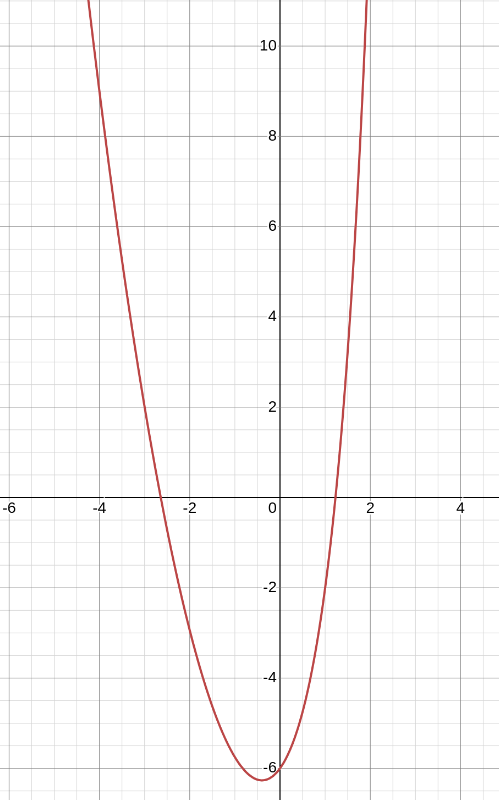
\includegraphics[scale=0.5]{ ./figures/1.png }
    % \end{center}
    \bigbreak \noindent 
    \textit{Then we will use 2 different $x_1$, at -3 and 3}

    \bigbreak \noindent \bigbreak \noindent 
    \subsection{Antiderivitates}
    \begin{itemize}
      \item Know what it means to be an Antiderivitate and how to find them
      \item know the most common Antiderivitates
      \item understand +C
      \item know why 
        \begin{align*}
          x^{\frac{1}{3}} \\ 
          = \frac{3}{4}x^{\frac{4}{3}}
        .\end{align*}
      \item and 
        \begin{align*}
          2y^{2} \\
          = \frac{2}{3}y^{3}
        .\end{align*}
      \item Know that \begin{align*}
        x^{-1} \\
        = \ln{\abs{x}}
      .\end{align*}
    \end{itemize}
     \pagebreak \bigbreak \noindent 
     Common Antiderivitates:
     \bigbreak \noindent 
     \begin{itemize}
      \item Exponential      
    \begin{itemize}
      \item $x^{n} = \frac{x^{n+1}}{n+1} + C$
      \item $e^{x} = e^{x} + C$
      \item $a^{x} = \frac{a^{x}}{\ln{a}} + C$
      \item $\frac{1}{x} = \ln{\abs{x}} + C$
      \item $\ln{x} = x\ln{x} - x + C$
      \item $\log_{a}{x} = \frac{x}{\ln{a}}(\ln{x} - 1) + C $
    \end{itemize}
    \bigbreak \noindent \bigbreak \noindent
  \item Trig:
    \begin{itemize}
      \item $\sin{x} = -\cos{x} +  C$
      \item $\cos{x} = \sin{x} + C$
      \item $\tan{x} = \ln{\abs{\sec{x}}} + C$
      \item $\csc{x} = \ln{\abs{\csc{x}-\cot{x}}} + C $
      \item $\sec{x}  = \ln{\abs{\sec{x}+\tan{x}}} + C$
      \item $\cot{x} = \ln{\abs{\sin{x}}} + C$
      \item $\sin^{2}{x} = \frac{1}{2}x-\frac{1}{4}\sin{2x} + C$
      \item $\cos^{2}{x}= \frac{1}{2}x+\frac{1}{4}\sin{2x} + C$
      \item $\tan^{2}{x}= -x + \tan{x} + C $
      \item $\csc^{2}{x}= -\cot{x} + C$
      \item $\sec^{2}{x} =\tan{x} + C$
      \item $\cot^{2}{x} =-x  - \cot{x} + C$
    \end{itemize}
    \bigbreak \noindent \bigbreak \noindent
  \item Hyperbolic Trig
    \begin{itemize}
      \item $\sinh{x} = \cosh{x} + C$
      \item $\cosh{x} = \sinh{x} + C$ 
      \item $\tanh{x} = \ln{\abs{\cos{x}}} + C$
      \item $csch{x} =  \ln{\abs{\tan{h}(\frac{1}{2}x)}} + C$ 
      \item $sech{x} = \tan^{-1}{(\sinh{(x)})} + C$
      \item $coth{x}= \ln{\abs{\sinh{x}}} + C $
      \item $csch^{2}{x} = -\coth{x}+ C$
      \item $sech^{2}{x} = \tanh{x} + C$
    \end{itemize}
    \end{itemize}


    \bigbreak \noindent \bigbreak \noindent 
    \subsection{derivative of hyperbolic trig fuctions}
    \begin{itemize}
      \item $\sinh{x}$ = $\cosh{x} $
      \item $\cosh{x}$ = $\sinh{x} $
      \item $\tanh{x} = \  $sech$^{2}$$x $
      \item sech $x $ = \ -sech $x$ $\tanh{x} $
      \item csch $x$ = \ -csch $x$ $\coth{x}$
      \item $\coth{x}$ = -csch$^{2}x$
    \end{itemize}
    \bigbreak \noindent 
    \textbf{lnx}
    \begin{itemize}
      \item when you have f(x) like:
        \begin{align*}
          f(x) = 3x^{-2}-7x^{-1}+6
        .\end{align*}
        \bigbreak \noindent 
        \textit{you can see if we tried to find F(x), by adding 1 to -1, we would get:}
        \begin{align*}
          \frac{-7^{0}}{0}
        .\end{align*}
        \bigbreak \noindent 
        \textit{Which is a problem, so instead, the Antiderivitive would be $-7\ln{\abs{x}}$}, this is because
        \begin{align*}
          \frac{d}{dx} -7\ln{x}\\ = -\frac{7}{x}
        .\end{align*}
        \bigbreak \noindent 
        \textit{And don't forget the absolute value bars}
    \end{itemize}

    \bigbreak \noindent \bigbreak \noindent
    \subsection{Sigma notation}
    \bigbreak \noindent 
    \begin{itemize}
      \item Know properties of summation:
      \begin{itemize}
           \item $\summation{n}{i=m}c \cdot a_i = c\summation{n}{i=m} a_{i}$, where c is a constant
          \item $\summation{n}{i=m} (a_{i} + b_{i})= \summation{n}{i=m} a_{i} + \summation{n}{i=m} b_{i} $
          \item $\summation{n}{i=m} (a_{i} - b_{i})= \summation{n}{i=m} a_{i} - \summation{n}{i=m} b_{i} $
          \item $\summation{n}{i=1} 1=n $
          \item $\summation{n}{i=1} c=c \cdot n $, where c is a constant
          \item $\summation{n}{i=1} i= \frac{n(n+1)}{2} $
          \item $\summation{n}{i=1}i^{2} = \frac{n(n+1)(2n+1)}{6} $
          \item $\summation{n}{i=1}i^{3}=\bigg[\frac{n(n+1)}{2}\bigg]^{2} $
      \end{itemize}
      \item Know what is means to be a telescoping sum and how to evaluate it.
      \item Know how to eval limits of summation, recall that if you have the limit as n -$>$ infinty, of a rational function whos degress are equal, evaluate the limit
        by taking the ration of the leading coefficients.
    \end{itemize}

    \bigbreak \noindent \bigbreak \noindent 
    \subsection{Area and Distance Problem}
    \begin{itemize}
      \item Know the definition for the area under the curve. 
    \end{itemize}
         \begin{align*}
       A = \lim_{n \to \infty}{R_{n}} = \lim_{n \to \infty}{[\Delta xf(x_{1}) + \Delta xf(x_{2}) + ... + \Delta xf(x_{n})]}
     .\end{align*}
     \begin{center}
       or
     \end{center}
      \begin{align*}
       A = \lim_{n \to \infty}{L_{n}} = \lim_{n \to \infty}{[\Delta xf(x_{0}) + \Delta xf(x_{1}) + ... + \Delta xf(x_{n-1})]}
     .\end{align*}
     \begin{center}
       or
     \end{center}
     \begin{align*}
       A = \lim_{n \to \infty}{[\Delta xf(x_{1}^{*}) + ... + \Delta xf(x_{n}^{*})]}
     .\end{align*}
     \bigbreak \noindent 
     Where $x_{i}^{*}$ is any number in the $i$th interval.
     \nt{$\Delta x =$ Base of each rectangle
       \bigbreak \noindent 
       Find $\Delta x$ with $\frac{b-a}{n}$, on [a,b]
     }
     \bigbreak \noindent 
     \begin{itemize}
       \item And the sigma versions:
     \end{itemize}
      \begin{itemize}
       \item $A = \lim\limits_{n \to \infty}{\summation{n}{i=1}\ \ \Delta xf(x_{i})} $ (Right endpoints)
       \item $A = \lim\limits_{n \to \infty}{\summation{n}{i=1}\ \ \Delta xf(x_{i-1})} $ (Left endpoints)
       \item $A = \lim\limits_{n \to \infty}{\summation{n}{i=1}\ \ \Delta xf(x_{i}^{*})} $ (Arbitrary partiton)
     \end{itemize}

     \bigbreak \noindent 
     \nt{The one with the star denotes not using left or right endpoints}
     \bigbreak \noindent 
     \begin{itemize}
       \item Know how to find $\Delta x$
         \begin{align*}
           \Delta x = \frac{b-a}{n}
         .\end{align*}
        \item Know how to find $x_i$ (right endpoints)
          \begin{align*}
            x_{i} = a + i \Delta x
          .\end{align*}
        \item Know how to find area with a fixed number of rectangles.
          \begin{itemize}
            \item Find $\Delta x $
            \item multiply $\Delta x$ by the sum of all the heights of the rectangles.
          \end{itemize}
     \end{itemize}
     \bigbreak \noindent \bigbreak \noindent
     Notes for riemann sum:
     \begin{itemize}
       \item Say we are using right endpoints with $n=4$, imagine we had the number line:
      \begin{figure}[ht]
          \centering
          \incfig{nlinettt}
          \label{fig:nlinettt}
      \end{figure}
      \begin{itemize}
        \item Since we are using right endpoints with $n=4$, we only use $\frac{5}{4}$ onward
        \item If we were using left endpoints, we would use $1$ to $\frac{7}{2}$
      \end{itemize}
       \end{itemize}


     \bigbreak \noindent \bigbreak \noindent 
     \subsection{Definite Integrals}
      \begin{itemize}
        \item Know: 
          \begin{align*}
            \int_{a}^{b}f(x)dx = \lim\limits_{n \to \infty}{\summation{n}{i=1}\ \ \Delta xf(x_{i}^{*})}
          .\end{align*}
        \item Know riemann sum:
          \begin{align*}
            \summation{n}{i=1}\ \ \Delta xf(x_{i})
          .\end{align*}
        \item Know the properties of integrals:
          \begin{itemize}
            \item $\int_{a}^{b} cdx = c(b-a) $ 
            \item $\int_{a}^{b}cf(x)dx = c \cdot \int_{a}^{b}f(x)dx $
            \item $\int_{a}^{b}[f(x) + g(x)]dx = \int_{a}^{b}f(x)dx + \int_{a}^{b}g(x)dx$
            \item $\int_{a}^{b}[f(x) - g(x)]dx = \int_{a}^{b}f(x)dx - \int_{a}^{b}g(x)dx$
            \item $\int_{a}^{c}f(x)dx = \int_{a}^{b}f(x)dx + \int_{b}^{c}f(x)dx $
            \item if $f(x) \geq 0$ for all $a \leq x \leq b$, then $\int_{a}^{b}f(x)dx \geq  0 $
            \item if $f(x) \geq g(x) $ for all $a \leq x \leq b$, then $\int_{a}^{b}f(x)dx \geq \int_{a}^{b}g(x)dx $
            \item if $m \leq f(x) \leq M $ for $a \leq x \leq b$, then $m(b-a) \leq \int_{a}^{b}f(x)dx \leq M(b-a)$
          \end{itemize}
          \bigbreak \noindent 
        \item Know how to find midpoints
          \begin{itemize}
            \item Make number line with right endpoints, then find the middle value of each interval
            \item If given an interval say, [1,3], and your asked to find midpoints, first plot number line with right endpoints. Then divide $\Delta x$ by 2 and add this number to each left point. Note that $\Delta x$ will remain the same when you find the riemann sum.
          \end{itemize}
        \item Know when you have equations for geometric shapes (circle, half cirle, line)
          \bigbreak \noindent 
        \item integral with the same bounds is \textbf{zero}
        \item Know how to split up integrals like
          \begin{align*}
            \int_{-1}^{2}\ (x-8\abs{x})\ dx
          .\end{align*}
          \begin{itemize}
            \item Set up piecewise
          \end{itemize}
          \begin{align*}
            x= 0\ \text{*Set whats inside abs = 0 to see where sign flips}
          .\end{align*}
               \begin{equation}
                =
                    \begin{cases}
                        x & \text{if } x \geq 0 \\
                        -x & \text{if } x < 0 
                    \end{cases}
                \end{equation}
              \item split integral
                \begin{align*}
                  \int_{-1}^{0}\ x-8(-x)\ dx + \int_{0}^{2}\ x-8x\ dx
                .\end{align*}
              \item Then evaluate
      \end{itemize}

      \bigbreak \noindent \bigbreak \noindent 
      \subsection{The Fundemental theorem of calculus}
      \begin{itemize}
        \item Know
          \begin{align*}
            Part\ 1:\ \frac{d}{dx}\int_{a}^{x}\ f(t)\ dt  = f(x), a \leq x \leq b         \\
            Part\ 2:\ \int_{a}^{b}\ f(x)\ dx = F(b) - F(a)\ where\ F^{\prime} = f. \\
            and \\
            \int_{a}^{b}\ f(x)\ dx = -\int_{b}^{a}\ f(x)\ dx
        .\end{align*}
        \smallbreak \noindent
        \item Know that you have to multiply by the derivative of the upper limit when you substitute for part 1
        \item Know how to split up integrals asked to find the derivative and if given something like:
          \begin{align*}
            F(x) = \int_{x}^{x^{2}}\ e^{t^{7}}\ dx
          .\end{align*}
          \begin{itemize}
            \item so this would end up
              \begin{align*}
                F^{\prime}(x) = \frac{d}{dx}\int_{x}^{0}\ e^{t^{7}}\ dt + \frac{d}{dx}\int_{0}^{x^{2}}\ e^{t^{7}}\ dt
              .\end{align*}
            \item and we would have to flip our limits of integration such that our upper limit is a function of x
              \begin{align*}
                F^{\prime}(x) = \frac{d}{dx}-\int_{0}^{x}\ e^{t^{7}}\ dt + \frac{d}{dx}\int_{0}^{x^{2}}\ e^{t^{7}}\ dt \\
                F^{\prime}(x) = e^{x^{7}} + e^{14} \cdot 2x \\
                 = e^{x^{7}} + 2xe^{14}\\
              .\end{align*}
          \end{itemize}
        \smallbreak \noindent
      \item Know the notation
        \begin{itemize}
          \item If given:
            \begin{align*}
              g(x) = \int_{0}^{x}\ \sqrt{t^{3} + t^{5}}\ dt
            .\end{align*}
          \item Notation for $g^{\prime}$ (using part 1) would be:
            \begin{align*}
              g^{\prime}(x) = \frac{d}{dx}\ \int_{0}^{x}\ \sqrt{t^{3} + t^{5}}\ dt \\
              = \sqrt{x^{3} + x^{5}}
            .\end{align*}
          \item definite integrals do not get +C
        \end{itemize}
      \end{itemize}

      \bigbreak \noindent \bigbreak \noindent 
      \subsection{Indefinite Integrals}
      \begin{itemize}
        \item  Indefinite Integrals are essentially just asking for the Antiderivitate, do not forget +C
        \item review common Antiderivitates
        \item know how to indeterminate antiderivative for inverse trig
        \item Know this antiderivative:
          \begin{align*}
            F(x) = 5^{x} \\
            f(x) = \frac{5^{x}}{\ln{5}} 
          .\end{align*}
          \begin{center}
            Because:
          \end{center}
          \begin{align*}
            \frac{d}{dx}\frac{5^{x}}{\ln{5}} \\
            =\frac{1}{\ln{5}}\bigg[5^{x}\bigg] \\
            = \frac{1}{\ln{5}} \bigg[5^{x} \cdot \ln{5}\bigg] \\
            = \frac{5^{x} \cdot \ln{5}}{\ln{5}} \\
            \boxed{= 5^{x}}
          .\end{align*}
      \end{itemize}

      \bigbreak \noindent \bigbreak \noindent
      \subsection{Velocity Functions with integrals}
      \bigbreak \noindent 
      If given:
      \begin{align*}
        v(t) = 3t-8,\ 0 \leq t \leq 3
      .\end{align*}
      \begin{itemize}
        \item Know that to find displacement: 
          \begin{align*}
            \int_{0}^{3}\ 3t-8\ dt
          .\end{align*}
        \item To find distance traveled:
          \begin{align*}
            \int_{0}^{3}\ \abs{3t-8}\ dx
          .\end{align*}
          \begin{itemize}
            \item So you must write as piecewise and split up the integral (add them)
          \end{itemize}
      \end{itemize}

      \pagebreak \bigbreak \noindent
      \subsection{The Substitution Rule (u-sub)}
      \bigbreak \noindent \bigbreak \noindent
      If $u=g(x)$ is differentiable and its range $\in I $ and $f $ is continuous on $I$, then
      \begin{align*}
        \int f(g(x))g^{\prime}(x)\ dx = \int f(u)\ du
      .\end{align*}
      \bigbreak \noindent \bigbreak \noindent
      \textbf{\textit{\underline{Process:}}}
      \begin{enumerate}
        \item Make a decent choice of what to let u equal
        \item Change our integral from being in terms of $x$, to in terms of $u$
        \item Integrate $\int f(u)\ du $
        \item Change back to $x$
      \end{enumerate}
      \bigbreak \noindent \bigbreak \noindent
      \nt{Also include the constant in your u sub, if it is attached to the function you let u equal,
        Also note for rational trig functions, you can move trig functions from upstairs or downstairs based on their reciprical function, for example, a $\cos^{2}{x}$ in the denominator can be
        moved upstairs as $\sec^{2}{x}$
      }
      \bigbreak \noindent \bigbreak \noindent
      \textbf{\textit{\underline{Notes:}}}
      \begin{itemize}
       \item Our goal with u-sub is to let u equal some function in our composition of functions, such that if we derive that function, we get back something that is also in our integrand
        \item Say we have something like:
          \begin{align*}
            \int \sec^{2}{\theta }\ d\theta  \\ 
            Let\ u = 8\theta  \\
            du = 8d\theta  \\
            \frac{1}{8}du = d\theta 
          .\end{align*}
        \item Know that you can rewrite equations like:
          \begin{align*}
            \int \frac{(\ln{x})^{36}}{x}\ dx \\
            as: \int \frac{1}{x}(\ln{x})^{36}\ dx
          .\end{align*}
        \item Say we have:
          \begin{align*}
            -\frac{1}{2} \int_{0}^{-1}\ e^{u}\ du
          .\end{align*}
          \begin{itemize}
            \item We can flip the limits of integration to remove the negative sign. So we will have:
          \end{itemize}
            \begin{align*}
              \frac{1}{2}\int_{-1}^{0}\ e^{u}\ du
            .\end{align*}
          \item Look out for being able to turn antiderivative into inverse trig functions.
            \begin{itemize}
              \item Say we have:
            \begin{align*}
              \int \frac{x^{7}}{1+x^{16}}\ dx
            .\end{align*}
          \item Don't let $u=1+x^{8} $, we could do this by turning $x^{16}\ into\ (x^{8})^{2}$, but instead, just let $u=x^{8}$. We do this because it ends up like:
            \begin{align*}
             \frac{1}{8}du = x^{7}dx  
            .\end{align*}
          \item So when we sub we get that nice arctan antiderivative, just something to look out for.
            \begin{align*}
              \frac{1}{8}\int \frac{1}{1+u^{2}}\ du
            .\end{align*}
            \end{itemize}
          \item Note that we can write:
            \begin{align*}
              e^{2x}
            .\end{align*}
            \begin{itemize}
              \item as 
            \end{itemize}
            \begin{align*}
              (e^{x})^{2}
            .\end{align*}
      \end{itemize}

      \bigbreak \noindent \bigbreak \noindent
       \textbf{\textit{\underline{Definite Integrals with u-sub}}} 
      \begin{enumerate}
        \item Find what u is going to equal
        \item Find u(a) and u(b) 
        \item make u-sub and use u(a) and u(b) as limits of integration
        \item find antiderivative and evaluate at new limits
      \end{enumerate}
      \bigbreak \noindent 
      \nt{For definite integrals, don't sub back in for u, just evalute integral with u still subbed}


      \pagebreak \bigbreak \noindent
      \subsection{Integrals of Symmetric functions:}
      \bigbreak \noindent \bigbreak \noindent
      \textbf{Sometimes you will run into integrals that are either impossible, or too difficult with u Substitution. For these cases we will look at Integrals of Symmetric Functions}
      \bigbreak \noindent \bigbreak \noindent
      \textbf{\textit{\underline{Even:}}} 
      \begin{align*}
        f(-x)  = f(x)\ then\ \int_{-a}^{a}\ f(x)\ dx  = 2 \int_{0}^{a}\ f(x)\ dx
      .\end{align*}
      \bigbreak \noindent \bigbreak \noindent
      \textbf{\textit{\underline{Odd:}}}
      \begin{align*}
        f(-x) = -f(x)\ then\ \int_{-a}^{a}\ f(x)\ dx = 0
      .\end{align*}

      \bigbreak \noindent \bigbreak \noindent
      \textbf{\textit{\underline{Notes:}}}
      \begin{itemize}
        \item If a function is even, you can replace your lower limit with zero and multiply the integral by 2
        \item if a function is odd, then the integral equals zero.
      \end{itemize}

      \bigbreak \noindent \bigbreak \noindent
      \textbf{\textit{\underline{Figures:}}}
      \begin{figure}[ht]
          \centering
          \incfig{fig1even}
          \incfig{fig2even}
          \label{fig:fig1even}
      \end{figure}

      \pagebreak \bigbreak \noindent 
      \subsection{The precise definition of a limit}
      \bigbreak \noindent 
      \textbf{Definition. }  We say (formally):
      \begin{align*}
        \lim\limits_{x \to a}{f(x) = L} \iff \forall \varepsilon > 0, \exists\ \delta > 0\ |\ 0 < \abs{x-a} < \delta \rightarrow \abs{f(x) - L} < \epsilon
      .\end{align*}
      \bigbreak \noindent 
      In simpler terms... We say: $ \lim\limits_{x \to a}{f(x) = L}$ if for every $\varepsilon > 0$ there is a $\delta > 0$ s.t if $\abs{x-a}<\delta$ then $\abs{f(x) - L} < \epsilon$
      \bigbreak \noindent 
      Consider the graph...
      \bigbreak \noindent 
      \begin{minipage}[]{0.47\textwidth}
         \incfig{graph111}
      \end{minipage}
      \begin{minipage}[]{0.47\textwidth}
        Use the graph of $f$ to find a number $\delta$ s.t if $0 < \abs{x-3}<\delta$ then $\abs{f(x) - 2} < 0.5$ 
        \bigbreak \noindent 
        \textbf{Solution.} 
        \begin{align*}
          &\abs{2.6 -3} = 0.4 \\
          &\abs{3.8 - 3} = 0.8
        .\end{align*}
        We choose the smaller value of $\delta $ to ensure that we are within the window. Thus we say:
        \begin{align*}
          &\delta = min(0.4, 0.8) \\
          &=0.4
        .\end{align*}
      \end{minipage}
      \bigbreak \noindent 
      Furthermore, let's prove using $\varepsilon$,\ $\delta$ definition of a limit.
      \begin{align*}
        \lim\limits_{x \to -1.5}{\frac{9-4x^{2}}{3+2x}} =6
      .\end{align*}
      \bigbreak \noindent 
      \textbf{Solution.} First we need to find $\delta$. Thus, Let $\varepsilon > 0 $. We need to find $\delta >0$ s.t whenever $\abs{x-(-1.5)} < \delta$, $\abs{f(x) - 6} < \epsilon$
      \begin{align*}
        &\implies \bigg|\frac{9-4x^{2}}{3+2x} -6\bigg| < \varepsilon
      .\end{align*}
      Our goal is to have $\abs{x+1.5}$ appear
      \begin{align*}
        \therefore &\bigg|\frac{(3+2x)(3-2x)}{3+2x} -6\bigg| < \varepsilon \\
        & |3-2x-6| < \varepsilon \\
        & \abs{-2x-3} < \varepsilon \\
        & \bigg|-2\bigg(x+\frac{3}{2}\bigg)\bigg| < \varepsilon \\
        &\abs{-2}\abs{x+1.5}<\varepsilon \\
        &\abs{x+1.5} < \frac{\varepsilon}{2}
      .\end{align*}
      Thus we choose $\delta = \frac{\varepsilon}{2} $
      \pagebreak \bigbreak \noindent 
      \pf{Proof}{
        Let $\varepsilon > 0$ be arbitrary. Choose $\delta < \frac{\varepsilon}{2}$. Assume $\bigg|x+1.5\bigg| < \frac{\varepsilon}{2}$
        
        Now let's examine $\bigg|\frac{9-4x^{2}}{3+2x}-6\bigg| $
        \begin{align*}
          &\bigg|\frac{9-4x^{2}}{3+2x}-6\bigg|  \\
            &\abs{-2}\abs{x+1.5} \\
          & \bigg|-2\bigg(x+\frac{3}{2}\bigg)\bigg| \\
          &2\abs{x+1.5}\\
        .\end{align*}
        We know that $\abs{x+1.5} < \frac{\varepsilon}{2}$. Thus, $2\abs{x+1.5} < 2\cdot \frac{\varepsilon}{2}$. From this we can conclude 
        \begin{align*}
          \bigg|\frac{9-4x^{2}}{3+2x}-6\bigg| < \varepsilon
        .\end{align*}
        \bigbreak \noindent 
        \ep
      }

      \pagebreak \bigbreak \noindent 
      \subsection{The squeeze theorem}
      \bigbreak \noindent 
      \textbf{Definition.} The squeeze theorem, proves very useful for establishing basic trigonometric limits. This theorem allows us to calculate limits by “squeezing” a function, with a limit at a point $a$ that is unknown, between two functions having a common known limit at $a$
      \bigbreak \noindent 
      \begin{thrm}
       Let \( f(x) \), \( g(x) \), and \( h(x) \) be defined for all \( x \neq a \) over an open interval containing \( a \). If
      \[ f(x) \leq g(x) \leq h(x) \]
      for all \( x \neq a \) in an open interval containing \( a \) and
      \[ \lim_{x \to a} f(x) = L = \lim_{x \to a} h(x) \]
      where \( L \) is a real number, then \( \lim_{x \to a} g(x) = L \).
      \end{thrm}
      \bigbreak \noindent 
      Dealing with the squeeze theorem suggests that we are going to be manipulating inequalities. Thus, I shall provide a brief rundown of rules and guidelines to consider.
      \bigbreak \noindent 
      \begin{enumerate}
        \item \textbf{Addition and Subtraction:}
        \begin{itemize}
            \item If \(a < b\), then \(a + c < b + c\) and \(a - c < b - c\) for any real number \(c\).
        \end{itemize}
        
        \item \textbf{Multiplication and Division with Positive Numbers:}
        \begin{itemize}
            \item If \(a < b\) and \(c > 0\), then \(ac < bc\) and \(a/c < b/c\).
            \item If \(a > b\) and \(c > 0\), then \(ac > bc\) and \(a/c > b/c\).
        \end{itemize}

        \item \textbf{Multiplication and Division with Negative Numbers:}
        \begin{itemize}
            \item If \(a < b\) and \(c < 0\), then \(ac > bc\) and \(a/c > b/c\). (Notice the inequality sign flips.)
            \item If \(a > b\) and \(c < 0\), then \(ac < bc\) and \(a/c < b/c\).
        \end{itemize}

        \item \textbf{Multiplication by Variables:}
        \begin{itemize}
            \item If you multiply or divide both sides of an inequality by a variable, and you don't know the variable's sign, you cannot determine the direction of the inequality without additional information.
        \end{itemize}

        \item \textbf{Compound Inequalities:}
        \begin{itemize}
            \item For \(a < b < c\), \(a < b\) and \(b < c\). If you add (or subtract) a value to all parts, the relationships stay the same.
            \item For multiplication or division, handle with care. If you multiply all parts by a positive number, the relationships stay the same. If by a negative number, all inequality signs flip.
        \end{itemize}

        \item \textbf{Squaring Both Sides:}
        \begin{itemize}
            \item Be cautious. If \(0 \leq a < b\), then \(a^2 < b^2\). However, if \(a < b \leq 0\), then \(a^2 > b^2\).
        \end{itemize}

        \item \textbf{Taking Roots:}
        \begin{itemize}
            \item If \(a < b\) and both \(a\) and \(b\) are non-negative, then \(\sqrt{a} < \sqrt{b}\) for even roots. For odd roots, this holds even if \(a\) and \(b\) are negative.
        \end{itemize}

        \item \textbf{Absolutes:}
        \begin{itemize}
            \item \(|a| < b\) means \( -b < a < b\).
            \item \(|a| > b\) means \(a < -b\) or \(a > b\).
        \end{itemize}

        \item \textbf{Reciprocals:}
        \begin{itemize}
            \item If \(0 < a < b\), then \( \frac{1}{a} > \frac{1}{b} \).
            \item If \(a < b < 0\), then \( \frac{1}{a} < \frac{1}{b} \).
        \end{itemize}

        \item \textbf{Transitive Property:}
        \begin{itemize}
            \item If \(a < b\) and \(b < c\), then \(a < c\).
        \end{itemize}
    \end{enumerate}
      \bigbreak \noindent  \bigbreak \noindent 
      Now let's consider:
      \begin{align*}
        \lim\limits_{x \to -\infty}{\frac{4x^{2}-\cos{(5x)}}{x^{2}-7}}
      .\end{align*}
      \bigbreak \noindent 
      We know:
      \begin{align*}
        &-1 \leq \cos{x} \leq 1 \\
        \implies &-1 \leq\cos{(5x)} \leq 1
      .\end{align*}
      \bigbreak \noindent 
      Now our goal with the squeeze theorem is to manipulate this inequality such that the thing we have in the middle (in this case $\cos{(5x)}$) becomes the $f(x)$ in our limit expression.
      \bigbreak \noindent 
      Thus, we begin manipulating.
      \begin{align*}
        -1 \leq &\cos{(5x)} \leq 1 \\
        1 \geq -&\cos{(5x)} \geq -1 \quad \text{(Multiplying by -1)}  \\
        -1 \leq -&\cos{(5x)} \leq 1 \quad \text{(Rearranging)} \\
        -1+4x^{2} \leq 4x^{2}-&\cos{(5x)} \leq 1 \quad \text{(Adding $4x^{2}$)} \\
        \frac{-1+4x^{2}}{x^{2}-7} \leq &\frac{4x^{2}-\cos{(5x)}}{x^{2}-7} \leq \frac{1+4x^{2}}{x^{2}-7} \quad \text{(Dividing by $x^{2}-7$)}
      .\end{align*}
      Note: For \( x \to -\infty \), \( x^2 \) grows without bound, and it will be much larger in magnitude than the constant term 7. Therefore, \( x^2 \) dominates the behavior of the expression \( x^2 - 7 \), making it positive. Since \( x^2 - 7 \) is positive and you are dividing by this expression, you do not need to flip the inequality.
      \bigbreak \noindent 
      Now that we have manipulated this inequality to match our desired function, we can take the limit of the left and right sides
      \begin{align*}
        \lim\limits_{x \to -\infty}{\frac{-1+4x^{2}}{x^{2}-7}} \leq &\lim\limits_{x \to -\infty}{\frac{4x^{2}-\cos{(5x)}}{x^{2}-7}} \leq \lim\limits_{x \to -\infty}{\frac{1+4x^{2}}{x^{2}-7}} \\
        4 \leq &\lim\limits_{x \to -\infty}{\frac{4x^{2}-\cos{(5x)}}{x^{2}-7}} \leq 4 \\
        \therefore &\lim\limits_{x \to -\infty}{\frac{4x^{2}-\cos{(5x)}}{x^{2}-7}} = 4 \quad \text{(By squeeze theorem)}
      .\end{align*}

      \bigbreak \noindent 
      \subsection{Finding where a function is inc/dec (and local extrema)}
      \begin{itemize}
        \item Find the derivative
        \item Find critical points
          \begin{itemize}
            \item For polynomial, set equal to zero to find all $c$
            \item For a rational function, set numerator equal to zero, then find where denominator DNE. Make sure these solutions are within the domain of the original function
            \item Test $c$ on number line with $f^{\prime}(x)$ find intervals of increasing or decreasing
            \item Original function has local extreme at $f(c)$ if it goes from increasing to decreasing, or decreasing to increasing at $c$ (refer to derivative tests)
            \item if we have no $c$ we can use points where the function is undefined. (However cannot be local extrema)
          \end{itemize}
      \end{itemize}

      \pagebreak \bigbreak \noindent
      \begin{center}
        \section{Intro Statistics}
      \end{center}
      \line(1,0){490}
      \bigbreak \noindent 
      \phantomsection
      \addcontentsline{toc}{subsection}{Chapters 1-4}
      \subsection*{Chapters 1-4}
      \bigbreak \noindent 
      \begin{large}
        \textbf{Titles}
      \end{large}
      \bigbreak \noindent 
      \textbf{Chapter 1:}
        \begin{itemize}
          \item 1.1: Introduction to the Practice of Statistics
          \item 1.2: Observational Studies versus Designed Experiments
          \item 1.3: Simple Random Sampling
          \item 1.4: Other Effective Sampling Methods
          \item 1.5: Bias in Sampling
          \item 1.6: The Design of Experiments
        \end{itemize}
      \textbf{Chapter 2:}
        \begin{itemize}
          \item 2.1: Organizing Qualitative Data
          \item 2.2: Organizing Quantitative Data: The Popular Displays
          \item 2.4: Graphical Misrepresentations of Data
        \end{itemize}
      \textbf{Chapter 3:}
        \begin{itemize}
          \item 3.1: Measures of Central Tendency
          \item 3.2: Measures of Dispersion
          \item 3.3: Measures of Central Tendency and Dispersion from Grouped Data
          \item 3.4: Measures of Position
          \item 3.5: The Five-Number Summary and Boxplots
        \end{itemize}
      \textbf{Chapter 4:}
        \begin{itemize}
          \item 4.1: Scatter Diagrams and Correlation
          \item 4.2: Least-Squares Regression
          \item 4.3: Diagnostics on the Least-Squares Regression Line
          \item 4.4: Contingency Tables and Association
        \end{itemize}

        \pagebreak \bigbreak \noindent
        \begin{large}
          \textbf{Learning Objectives}
        \end{large}
        % \addcontentsline{toc}{subsubsection}{Learning Objectives}
        \bigbreak \noindent 
        \begin{itemize}
        \item \textbf{Obtain a simple random sample}
            \item \textbf{Explain the Sources of Bias in Sampling}
            \item \textbf{Describe the Characteristics of an Experiment (vocab)}
            \item \textbf{Explain the Steps in Designing an Experiment}
            \item \textbf{Explain the Completely Randomized Design}
            \item \textbf{Explain the Matched-Pairs Design}
            \item \textbf{Organize Qualitative Data in Tables}
            \item \textbf{Construct Bar Graphs}
            \item \textbf{Construct Pie Charts}
            \item \textbf{Organize Discrete Data in Tables}
            \item \textbf{Construct Histograms of Discrete Data}
            \item \textbf{Organize Continuous Data in Tables}
            \item \textbf{Construct Histograms of Continuous Data}
            \item \textbf{Draw Dot Plots}
            \item \textbf{Identify the Shape of a Distribution}
            \item \textbf{Describe What Can Make a Graph Misleading or Deceptive}
            \item \textbf{Determine the Arithmetic Mean of a Variable from Raw Data}
            \item \textbf{Determine the Median of a Variable from Raw Data}
            \item \textbf{Explain What It Means for a Statistic to be Resistant}
            \item \textbf{Determine the Mode of a Variable from Raw Data}
            \item \textbf{Determine the Range of a Variable from Raw Data}
            \item \textbf{Determine the Standard Deviation of a Variable from Raw Data}
            \item \textbf{Determine the Variance of a Variable from Raw Data}
            \item \textbf{Use the Empirical Rule to Describe Data That Are Bell-Shaped}
           \item \textbf{Approximate the Mean of a Variable from Grouped Data}
           \item \textbf{Compute the Weighted Mean}
           \item \textbf{Approximate the Standard Deviation from a Frequency Distribution}
           \item \textbf{Determine and Interpret z-Scores}
           \item \textbf{Interpret Percentiles}
           \item \textbf{Determine and Interpret Quartiles}
           \item \textbf{Determine and Interpret the Interquartile Range}
           \item \textbf{Check a Set of Data for Outliers}
            \item \textbf{Determine the Five-Number Summary}
            \item \textbf{Draw and Interpret Boxplots}
            \item \textbf{Draw and Interpret Scatter Diagrams}
            \item \textbf{Describe the Properties of the Linear Correlation Coefficient}
            \item \textbf{Compute and Interpret the Linear Correlation Coefficient}
            \item \textbf{4Determine Whether a Linear Relation Exists between Two Variables}
            \item \textbf{Explain the Difference between Correlation and Causation}
            \item \textbf{Find the Least-Squares Regression Line and Use the Line to Make Predictions}
            \item \textbf{Interpret the Slope and the y-Intercept of the Least-Squares Regression Line}
            \item \textbf{Compute the Sum of Squared Residuals}
            \item \textbf{Compute and Interpret the Coefficient of Determination}
            \item \textbf{Perform Residual Analysis on a Regression Model}
            \item \textbf{Identify Influential Observations}
            \item \textbf{Compute the Marginal Distribution of a Variable}
            \item \textbf{Use the Conditional Distribution to Identify Association Among Categorical Data}
            \item \textbf{Explain Simpson's Paradox}
        \end{itemize}


        \pagebreak \bigbreak \noindent
      \begin{large}
        \textbf{Vocab}
      \end{large}
      % \addcontentsline{toc}{subsubsection}{Vocab}
    \begin{itemize}
        \item \textbf{Population:} The entire group to be studied is called the population.
        \item \textbf{Sample:} In statistics, it is often impractical or impossible to get access to the entire \textbf{population}, which is why we only look at a \textbf{sample.} A sample is a \textbf{subset} of the population being studied.
        \item \textbf{Individual:} An individual is a person or object that is a member of the population being studied.
        \item \textbf{Statistic:} A statistic is a numerical summary of a sample.
        \item \textbf{Descriptive Statistics:} Descriptive statistics consist of organizing and summarizing data. Descriptive statistics describe data through numerical summaries, tables, and graphs.
        \item \textbf{Inferential Statistics:} inferential Statistics uses methods that take a result from a sample, extend it to the population, and measure the reliability of the result.
        \item \textbf{Parameter:} A parameter is a numerical summary of a population.
        \item \textbf{Variables:} The characteristics of the individuals in a study. Variables vary, which means they can take on different values.
        \item \textbf{Constants:} Variables that do not vary. Inferential statistics is not necessary with constants.
        \item \textbf{Qualitative, or categorical variables} allow for the classification of individuals base on some attribute or characteristic.
        \item \textbf{Quantitative variables} provide numerical measures of individuals. The values of a quantitative variable can be added or subtracted and provide meaningful results.
        \item A \textbf{discrete variable} is a quantitative variable that has either a finite number of possible values or a countable number of possible values. A discrete variable cannot take on every possible value between any two possible values.
        \item A \textbf{continuous variable} is a quantitative variable that has an infinite number of possible values that are not countable. A continuous variable may take on every possible value between any two values. Continuous variables typically result from measurement. Continuous variables are often rounded. If a certain make of car gets 24 miles per gallon (mpg) of gasoline, its miles per gallon must be greater than or equal to 23.5 and less than 24.5, or $23.5 \leq mpg \leq 24.5$
        \item The list of observed values for a variable is \textbf{data.}
        \item \textbf{Qualitative data} are observations corresponding to a \textbf{qualitative variable.}
        \item \textbf{Quantitative data} are observations corresponding to a quantitative variable.
        \item \textbf{Discrete data} are observations corresponding to a discrete variable.
        \item \textbf{Continuous data} are observations corresponding to a continuous variable.
            \item \textbf{Explanatory Variable:} An explanatory variable, also known as an independent variable or predictor variable, is a variable that is manipulated or controlled by researchers in an experiment or study. It is the variable that is hypothesized to have an impact on the outcome or dependent variable. 
            \item \textbf{Lurking variable}: An explanatory variable that was not considered in a study, but that affects the value of the response variable.
            \item \textbf{Response Variable}: The response variable, also known as the dependent variable or outcome variable, is the variable that is measured or observed to determine the effect or response of the explanatory variable(s). It is the variable that researchers are interested in studying or predicting. 
            \item \textbf{Confounding:} Occurs when the effects of two or more explanatory variables are not separated. Therefore, any relation that may exist between an explanatory variable and the response variable may be due to some other variable or variables not accounted for in the study.
            \item \textbf{Census:} List of individuals in a population along with certain characteristics of each individual.
            \item \textbf{Random Sampling:} The process of using chance to select individuals from a population to be included in the sample.
            \item \textbf{Simple Random Sampling:} A sample of size $n$  from a population of size $N $  is obtained through simple random sampling if every possible sample of size $n$  has an equal chance of occurring. The sample is then called a simple random sample.
                \begin{itemize}
                    \item $n < N $
                \end{itemize}
            \item \textbf{frame:} a list of all the individuals within the population.
            \item \textbf{Sample Without Replacement:} Once an individual is selected, the individual cannot be selected again.
            \item \textbf{Stratified sample}: is obtained by dividing the population into nonoverlapping groups called strata and then obtaining a simple random sample from each stratum. The individuals within each stratum should be homogenous (similar) in some way.
                \begin{itemize}
                    \item Within Stratified samples, the number of individuals sampled from each stratum should be proportional to the size of the strata in the population.
                \end{itemize}
            \item \textbf{Systematic sample} is obtained by selecting every $k$th individual from the population. The first individual selected corresponds to a number between 1 and $k$
            \item \textbf{Cluster sample} is obtained by selecting all individuals within a randomly selected collection or group of individuals.
            \item \textbf{Convenience sample:} the individuals are easily obtained and not based on randomness.
            \item \textbf{Bias:} If the results of the sample are not representative of the population. Sampling bias means that the technique used to obtain the sample's individuals tends to favor one part of the  population over another. Any convenience sample has sampling bias because the individuals are not chosen through a random sample.
            \item \textbf{Undercoverage:} Occurs when the proportion of one segment of the population is lower in a sample than it is in the population. This can result if the frame used to obtain the sample is incomplete or not representative of the population.
            \item \textbf{Sampling bias:} sampling bias is a bias in which a sample is collected in such a way that some members of the intended population have a lower or higher sampling probability than others. It results in a biased sample of a population in which all individuals, or instances, were not equally likely to have been selected
            \item \textbf{Nonresponse bias:} exists when individuals selected to be in the sample who do not respond to the survey have different opinions from those who do
                \begin{itemize}
                    \item This can be controlled with \textbf{callbacks}.
                    \item This can also be controlled with \textbf{rewards or incentives}
                \end{itemize}
            \item \textbf{Response bias:} Exists when the answers on a survey do not reflect the true feelings of the respondent.
            \item \textbf{Open Question:} Allows the respondent to choose his or her response
            \item \textbf{Closed Question:} requires the respondent to choose from a list of predetermined responses
            \item \textbf{Nonsampling errors:} result from undercoverage, nonresponse bias, response bias, or data-entry error. Such errors could also be present in a census.
            \item \textbf{Sampling error:} results from using a sample to estimate information about a population. This type of error occurs because a sample gives incomplete information about a population.
            \item \textbf{Experiment:} is a controlled study conducted to determine the effect of varying one or more explanatory variables or \textbf{factors} has on a response variable. 
            \item \textbf{Factor:} A variable whose effect on the response variable is to be assessed by the experimenter
            \item \textbf{Treatment:} Any combination of the values of the factors is called a treatment
            \item \textbf{Experimental Unit (or subject)} is a person, object or some other well-defined item upon which a treatment is applied
            \item \textbf{Control Group:} Serves as a baseline treatment that can be used to compare to other treatments.
            \item \textbf{Placebo:} is an innocuous medication, such as a sugar tablet, that looks, tastes, and smells like the experimental medication.
            \item \textbf{Blinding:} refers to nondisclosure of the treatment an experimental unit is receiving.
            \item \textbf{Single-blind} experiment is one in which the experimental unit (or subject) does not know which treatment he or she is receiving.
            \item \textbf{Double-blind} experiment is one in which neither the experimental unit nor the researcher in contact with the experimental unit knows which treatment the experimental unit is receiving.
            \item \textbf{Design:} To design an experiment means to describe the overall plan in conducting the experiment. Conducting an experiment requires a series of steps.
            \item \textbf{Blocking:} Grouping together similar experimental units and then randomly assigning the experimental units within each group to a treatment is called 
            \item \textbf{completely randomized design:} is one in which each experimental unit is randomly assigned to a treatment.
            \item \textbf{matched-pairs design:} is an experimental design in which the experimental units are paired up. The pairs are selected so that they are related in some way (that is, the same person before and after a treatment, twins, husband and wife, same geographical location, and so on). There are only two levels of treatment in a matched-pairs design.
            \item \textbf{The relative frequency} is the proportion (or percent) of observations within a category and is found using the formula
            \item \textbf{Classes: } The Categories in which data is grouped
            \item \textbf{lower class limit:} the smallest value within the class 
            \item \textbf{upper class limit:} the largest value within the class 
            \item \textbf{Class Width: }  is the difference between consecutive lower class limits.
            \item A table is \textbf{open ended} if the first class has no lower class limit or the last class has no upper class limit
            \item \textbf{uniform distribution:} frequency of each value of the variable is evenly spread across the values of the variable. 
            \item \textbf{bell-shaped distribution:} highest frequency occurs in the middle and frequencies tail off to the left and right of the middle.
            \item \textbf{skewed right:} the tail to the right of the peak is longer than the tail to the left of the peak
            \item \textbf{skewed left:} tail to the left of the peak is longer than the tail to the right of the peak.
            \item \textbf{The arithmetic mean} of a variable is computed by adding all the values of the variable in the data set and dividing by the number of observations.
            \item \textbf{The population arithmetic mean}, $\mu$, (pronounced "mew"), is a parameter that is computed using data from all the individuals in a population.
            \item \textbf{The sample arithmetic mean}, $\bar{x}$ (pronounced x-bar"), is a statistic that is computed using data from individuals in a sample.
            \item \textbf{The median} of a variable is the value that lies in the middle of the data when arranged in ascending order. We use $M$  to represent the median.
            \item A numerical summary of data is said to be \textbf{resistant} if observations that are extreme (very large or small) relative to the data do not affect its value substantially.
                \begin{itemize}
                    \item So the median is resistant, but the mean is not resistant.
                \end{itemize}
            \item \textbf{The mode} of a variable is the observation of the variable that occurs most frequently in the data set.
                \begin{itemize}
                    \item If no observation occurs more than once, we say that the data have \textbf{no mode}.
                \end{itemize}
            \item \textbf{Bimodal:} If the data has two modes
            \item \textbf{Multimodal:} If the data has more than two modes
            \item \textbf{Dispersion:} Degree to which the data are spread out. 
            \item \textbf{Range:} The range, $r $, of a variable is the difference between the largest and smallest data value. That is,
                \textbf{Note:} Range is \textbf{not} resistant
            \item \textbf{Deviation about the mean:} a deviation refers to the difference between an individual data point and a central value, such as the mean or median. It represents how much a particular data point varies or deviates from the average or typical value in a data set. 
                \bigbreak \noindent 
                \textbf{Note:} The sum of the deviations about the mean always equals zero
            % \item \textbf{The population standard deviation} of a variable is the square root of the sum of squared deviations about the population mean divided by the number of observations in the population, $N$. The population standard deviation is symbolically represented by $\sigma$ (lowercase Greek sigma). The formula is given by:
            %     \textbf{Note:} Standard Deviation is \textbf{not} resistant
            % \item \textbf{The sample standard deviation}, $s $, of a variable is the square root of the sum of squared deviations about the sample mean divided by $n-1 $, where $n$  is the sample size. The formula is given as
            %     \textbf{Note:} Standard Deviation is \textbf{not} resistant
              \item \textbf{Standard Deviation:} Measure of dispersion. It gives us a sense of how much the individual values deviate or differ from the average (mean) value. The standard deviation and the mean together can tell you where most of the values in your frequency distribution lie if they follow a normal distribution (Empirical Rule).
            \item  we call $n-1$ the \textbf{degrees of freedom} because the first $n-1 $  observations have freedom to be any value, but the $n^{th}$ observation has no freedom. It must be whatever value forces the sum of the deviations about the mean to equal zero.
            \item The \textbf{variance}  It assesses the average squared difference between data values and the mean. Find my squaring $\sigma $ or $s$ \\
              \textbf{Note:} The units of measure in variance are squared values. So if the variable is measured in dollars, the variance is measured in dollars squared. This makes interpreting the variance difficult.
                \item \textbf{Coefficient of Variation:} The coefficient of​ variation, CV, is defined as the ratio of the standard deviation to the mean of a data set. The CV allows for a comparison in spread by describing the amount of spread per unit mean.
               \textbf{Note:} When converting units of​ measure, the coefficient of variation is unchanged.
             \item \textbf{Class Midpoint:} The class midpoint is the sum of consecutive lower class limits divided by 2
             \item \textbf{Approximate Population Mean (if we do not have access to the original data, ie data has been grouped (classed) and frequency chart has already been made)}
            \item \textbf{Approximate Sample Mean (if we do not have access to the original data, ie data has been grouped (classed) and frequency chart has already been made)}
            \item \textbf{The weighted mean}, $\overline{x}_{w}$, of a variable is found by multiplying each value of the variable by its corresponding weight, adding these products, and dividing this sum by the sum of the weights. It can be expressed using the formula
            \item \textbf{Approximate Population Standard Deviation (if we do not have access to the original data, ie data has been grouped (classed) and frequency chart has already been made)}
            \item \textbf{Approximate Sample Standard Deviation (if we do not have access to the original data, ie data has been grouped (classed) and frequency chart has already been made)}
             \item \textbf{The z-score} represents the distance that a data value is from the mean in terms of the number of standard deviations. We find it by subtracting the mean from the data value and dividing this result by the standard deviation.
                 \textbf{Note:} The Z-score is unitless. It has mean  0 and a standard deviation of 1 \\
                 \textbf{Round z-scores to the nearest hundredth}
             \item  The median is a special case of a general concept called the \textbf{percentile.}
             \item \textbf{the $k^{th}$  percentile,} denoted $P_{k} $,  of a set of data is a value such that $k $  percent of the observations are less than or equal to the value.
                \item The most common percentiles are \textbf{quartiles}, which divide data sets into fourths, or four equal parts.
                \item The \textbf{interquartile range, IQR,} is the range of the middle $50\% $  of the observations in a data set. That is, the IQR is the difference between the first and third quartiles and is found using this formula  
               \item \textbf{Outliers:} When analyzing data, we must check for extreme observations, called outliers. Outliers can occur by chance, because of errors in the measurement of a variable, during data entry, or from errors in sampling.
                \item \textbf{Fences} serve as cutoff points for determining outliers.
        \item \textbf{bivariate data:} data in which two variables are measured on an individual. For example, we might want to know whether the amount of cola consumed per week is related to a person's bone density. The individuals would be the people in the study, and the two variables would be the amount of cola consumed weekly and bone density.
        \item Two variables that are linearly related are \textbf{positively associated} when above-average values of one variable are associated with above-average values of the other variable (or below-average values of one variable are associated with below-average values of the other variable). That is, two variables are positively associated if, whenever the value of one variable increases, the value of the other variable also increases.
        \item Two variables that are linearly related are \textbf{negatively associated} when above-average values of one variable are associated with below-average values of the other variable. That is, two variables are negatively associated if, whenever the value of one variable increases, the value of the other variable decreases.
        \item The \textbf{linear correlation coefficient}, or Pearson product moment correlation coefficient, is a measure of the strength and direction of the linear relation between two quantitative variables. The Greek letter $\rho $ (rho) represents the population correlation coefficient, and $r $ represents the sample correlation coefficient. We present only the formula for the sample correlation coefficient.
        \item \textbf{The least-squares regression line} minimizes the sum of the squared errors (or residuals). This line minimizes the sum of the squared vertical distance between the observed values of $y$  and those predicted by the line, $\hat{y}$  (read “y-hat"). We represent this as $\sum residuals^{2}$
        \item The observed distance for this club-head speed is 274 yards. The difference between the observed and predicted values of y is the error, or \textbf{residual}.
            \begin{align*}
                Residual\ = observed - predicted
            .\end{align*}
        \item \textbf{The coefficient of determination}, $R^{2}$, measures the proportion of total variation in the response variable that is explained by the least-squares regression line.
            \begin{align*}
                R^{2} = r^{2}
            .\end{align*}
        \item \textbf{An influential observation} significantly affects the least-squares regression line's slope and/or y-intercept. (It also affects the value of the correlation coefficient.) Methods exist for determining whether a particular observation is influential; however, they are beyond the scope of this course. Nonetheless, we can still get a sense as to whether a particular observation is influential right now.
        \item the difference in our predicted value, and our actual value, is due to factors (variables) other than the club-head speed (wind speed and position of the ball on the club face, for example) and to random error. The differences just discussed are called \textbf{deviations}.
        \item \textbf{Total Deviation:} The deviation between the observed value, y, and mean value, $\overline{y} $, of the response variable.
            \begin{align*}
                &y - \overline{y} \\
                &Or: \text{Explained Deviation + Unexplained Deviation}
            .\end{align*}
        \item \textbf{Explained Deviation:} The deviation between the predicted value, $\hat{y} $, and mean value, $\overline{y} $, of the response variable.
            \begin{align*}
                \hat{y}-\overline{y}
            .\end{align*}
        \item \textbf{Unexplained Deviation:} The deviation between the observed value, y, and predicted value, $\hat{y} $, of the response variable
            \begin{align*}
                y - \hat{y}
            .\end{align*}
        \item     If a plot of the residuals against the explanatory variable shows the spread of the residuals increasing or decreasing as the explanatory variable increases, then a strict requirement of the linear model is violated.     This requirement is called \textbf{constant error variance}. The statistical term for constant error variance is \textbf{homoscedasticity}

        \item \textbf{Simpson's Paradox}, which describes a situation in which an association between two variables inverts or goes away when a third variable is introduced to the analysis.
        \end{itemize}

        \pagebreak \bigbreak \noindent
        \begin{large}
          \textbf{Charts and Graphs:}
        \end{large}
        \begin{itemize}
           \item \textbf{A frequency distribution} lists each category of data and the number of occurrences for each category of data.
           \item \textbf{A relative frequency distribution} lists each category of data together with the relative frequency.
             \item \textbf{A bar graph} is constructed by labeling each category of data on either the horizontal or vertical axis and the frequency or relative frequency of the category on the other axis. Rectangles of equal width are drawn for each category. The height of each rectangle represents the category's frequency or relative frequency.
            \item \textbf{A Pareto chart} is a bar graph whose bars are drawn in decreasing order of frequency or relative frequency.
            \item \textbf{A pie chart} is a circle divided into sectors. Each sector represents a category of data. The area of each sector is proportional to the frequency of the category.
            \item A \textbf{histogram} is constructed by drawing rectangles for each class of data. The height of each rectangle is the frequency or relative frequency of the class. The width of each rectangle is the same, and the rectangles touch each other.
            \item We draw a \textbf{dot plot} by placing each observation horizontally in increasing order and placing a dot above the observation each time it is observed.
             \item The \textbf{five-number summary} of a set of data consists of the smallest data value, $Q_{1} $  the median, $Q_{3} $  and the largest data value. We use the five-number summary to learn information about the extremes of the data set. The summary is organized as follows:
              \begin{center}
                 Minimum $Q_{1} $ $M$ $Q_{3} $  Maximum
              \end{center}
        \item \textbf{A scatter diagram} is a graph that shows the relationship between two quantitative variables measured on the same individual. Each individual in the data set is represented by a point in the scatter diagram. The explanatory variable is plotted on the horizontal axis, and the response variable is plotted on the vertical axis.
          \begin{itemize}
            \item A scatter plot is useful to determine if the presence of outliers causing an effect.
          \end{itemize}
        \item \textbf{A marginal distribution} of a variable is a frequency or relative frequency distribution of either the row or column variable in the contingency table.
        \item \textbf{A conditional distribution} lists the relative frequency of each category of the response variable, given a specific value of the explanatory variable in the contingency table.
        \end{itemize}


        \pagebreak \bigbreak \noindent
        \begin{large}
          \textbf{Formulas}
        \end{large}
        % \addcontentsline{toc}{subsubsection}{Formulas}
        \bigbreak \noindent 
        \begin{itemize}
                        \item \textbf{The relative frequency} is the proportion (or percent) of observations within a category. 
                \begin{align*}
                    Relative\ frequency = \frac{Frequency}{Sum\ of\ all\ frequency}
                .\end{align*}

                    \item \textbf{The population arithmetic mean}, $\mu$, (pronounced "mew"), is a parameter that is computed using data from all the individuals in a population.
                \begin{align*}
                    \mu = \frac{x_{1}+x_{2} + x_{N}}{N} = \frac{\summation{}{}x_{i}}{N}
                .\end{align*}
            \item \textbf{The sample arithmetic mean}, $\bar{x}$ (pronounced x-bar"), is a statistic that is computed using data from individuals in a sample.
                \begin{align*}
                    \bar{x} = \frac{x_{1}+x_{2} + x_{n}}{n} = \frac{\summation{}{}x_{i}}{n}
                .\end{align*}
            \item \textbf{The median} of a variable is the value that lies in the middle of the data when arranged in ascending order. We use $M$  to represent the median.
                \begin{itemize}
                    \item For odd $n$:
                        \begin{align*}
                            M = \frac{n+1}{2}
                        .\end{align*}
                    \item For even $n$:
                        \begin{align*}
                            M = Average\ of\ \frac{n}{2}, \frac{n}{2}+1
                        .\end{align*}
                \end{itemize}
            \item \textbf{Range:} The range, $r $, of a variable is the difference between the largest and smallest data value. That is,
                \begin{align*}
                    range = R = Largest\ data\ value- smallest\ data\ value
                .\end{align*}
            \item \textbf{Deviation:} a deviation refers to the difference between an individual data point and a central value, such as the mean or median. It represents how much a particular data point varies or deviates from the average or typical value in a data set. When can comopute a deviation with:
                \begin{align*}
                    Individual\ data\ point - mean
                .\end{align*}


            \item \textbf{The population standard deviation} of a variable is the square root of the sum of squared deviations about the population mean divided by the number of observations in the population, $N$. The population standard deviation is symbolically represented by $\sigma$ (lowercase Greek sigma). The formula is given by:
                \begin{align*}
                    \sigma = \sqrt{\frac{(x_{1} - \mu)^{2} + (x_{2}-\mu)^{2}+...+(x_{N}-\mu)^{2}}{N}} \\
                    = \sqrt{\frac{\summation{}{}(x_{i}-\mu)^{2} }{N}}
                .\end{align*}
                \textbf{Note:} Standard Deviation is \textbf{not} resistant
            \item \textbf{The sample standard deviation}, $s $, of a variable is the square root of the sum of squared deviations about the sample mean divided by $n-1 $, where $n$  is the sample size. The formula is given as
                \begin{align*}
                    s = \sqrt{\frac{(x_{1} - \overline{x})^{2}+(x_{2}-\overline{x})^{2}+...+(x_{n}-\overline{x})^{2}}{n-1}}\\
                    = \sqrt{\frac{\summation{}{}(x_{i}-\overline{x})^{2}}{n-1}}
                .\end{align*}
                \textbf{Note:} Standard Deviation is \textbf{not} resistant
            \item  \textbf{The population variance} is \textbf{$\sigma^{2}$} 
            \item \textbf{The Sample Variance} is $s^{2}$
             \item \textbf{Approximate Population Mean (if we do not have access to the original data, ie data has been grouped (classed) and frequency chart has already been made)}
                \begin{align*}
                    \mu =\frac{\sum x_i f_i}{\sum f_i} \\
                     =\frac{x_1 f_1+x_2 f_2+\cdots+x_n f_n}{f_1+f_2+\cdots+f_n}
                .\end{align*}
            where: $\quad x_i$ is the midpoint or value of the $i$ th class  \\
            $f_i$ is the frequency of the $i$ th class  \\
            $n$ is the number of classes
            \item \textbf{Approximate Sample Mean (if we do not have access to the original data, ie data has been grouped (classed) and frequency chart has already been made)}
                \begin{align*}
                    \overline{x} = \frac{\sum x_{i}f_{i}}{\sum f_{i}} \\
                     = \frac{x_{1}f_{1} + x_{2} f_{2} + ... +x_{n} f_{n}}{f_{1} + f_{2} + ... + f_{n}}
                .\end{align*}
            where: $\quad x_i$ is the midpoint or value of the $i$ th class  \\
            $f_i$ is the frequency of the $i$ th class  \\
            $n$ is the number of classes
            \item \textbf{The weighted mean}, $\overline{x}_{w}$, of a variable is found by multiplying each value of the variable by its corresponding weight, adding these products, and dividing this sum by the sum of the weights. It can be expressed using the formula
                \begin{align*}
                    \overline{x}_{w} = \frac{\sum w_{i}x_{i}}{w_{i}} = \frac{w_{1} + x_{1} + w_{2} + x_{2} + ... + w_{n} + x_{n}}{w_{1} + w_{2} + ... + w_{n}}
                .\end{align*}
                Where: \quad $w_{i}$ is the weight of the $i^{th}$ observation \\
                $x_{i}$ is the value of the $i^{th}$ observation.
            \item \textbf{Approximate Population Standard Deviation (if we do not have access to the original data, ie data has been grouped (classed) and frequency chart has already been made)}
                \begin{align*}
                    \sigma = \sqrt{\frac{\sum(x_{i} - \mu)^{2}f_{i}}{\sum f_{i}}}
                .\end{align*}
                Where: \quad  $x_{i}$ is the midpoint or value of the ith class \\
                $f_{i}$ is the frequency of the $i^{th}$ class
            \item \textbf{Approximate Sample Standard Deviation (if we do not have access to the original data, ie data has been grouped (classed) and frequency chart has already been made)}
                \begin{align*}
                    s = \sqrt{\frac{\sum(x_{i}-\overline{x})^{2}f_{i}}{\sum f_{i} -1}}
                .\end{align*}
                Where: \quad  $x_{i}$ is the midpoint or value of the ith class \\
                $f_{i}$ is the frequency of the $i^{th}$ class
             \item \textbf{The z-score} represents the distance that a data value is from the mean in terms of the number of standard deviations. We find it by subtracting the mean from the data value and dividing this result by the standard deviation.
                 \begin{itemize}
                     \item \textbf{Population Z-score}
                 \end{itemize}
                 \begin{align*}
                      z = \frac{x - \mu}{\sigma}
                 .\end{align*}
                 \begin{itemize}
                     \item \textbf{Sample Z-score}
                 \end{itemize}
                 \begin{align*}
                     z =\frac{x-\overline{x}}{s}
                 .\end{align*}
                 \textbf{Note:} The Z-score is unitless. It has mean  0 and a standard deviation of 1 \\
                 \textbf{Round z-scores to the nearest hundredth}
                \item The \textbf{interquartile range, IQR,} is the range of the middle $50\% $  of the observations in a data set. That is, the IQR is the difference between the first and third quartiles and is found using this formula  
                    \begin{align*}
                        IQR = Q_{3} - Q_{1}
                    .\end{align*}
                \item \textbf{Fences} serve as cutoff points for determining outliers.
                    \begin{align*}
                        Lower\ Fence\ = Q_{1} - 1.5\cdot IQR \\
                        Upper\ Fence\ = Q_{3} + 1.5\cdot IQR
                    .\end{align*}
        \item The \textbf{five-number summary} of a set of data consists of the smallest data value, $Q_{1} $  the median, $Q_{3} $  and the largest data value. We use the five-number summary to learn information about the extremes of the data set. The summary is organized as follows:
        \begin{center}
           Minimum $Q_{1} $ $M$ $Q_{3} $  Maximum
        \end{center}
        \item The \textbf{linear correlation coefficient}, or Pearson product moment correlation coefficient, is a measure of the strength and direction of the linear relation between two quantitative variables. The Greek letter $\rho $ (rho) represents the population correlation coefficient, and $r $ represents the sample correlation coefficient. We present only the formula for the sample correlation coefficient.
            \begin{align*}
                r =\frac{\sum\left(\frac{x_i-\bar{x}}{s_x}\right)\left(\frac{y_i-\bar{y}}{s_y}\right)}{n-1}
            .\end{align*}
            Where:
            \bigbreak \noindent 
                $x_i$ is the $i$ th observation of the explanatory variable \\
                $\overline{x}$ is the sample mean of the explanatory variable \\
                $s_{x} $is the sample standard deviation of the explanatory variable \\
                $y_i$ is the $i$ th observation of the response variable \\
                $\overline{y}$ is the sample mean of the response variable \\
                $\mathbf{S}_y$ is the sample standard deviation of the response variable \\
                $n$ is the number of individuals in the sample

        \item \textbf{The least-squares regression line} minimizes the sum of the squared errors (or residuals). This line minimizes the sum of the squared vertical distance between the observed values of $y$  and those predicted by the line, $\hat{y}$  (read “y-hat"). We represent this as $\sum residuals^{2}$
            \begin{align*}
               \hat{y} = b_{1}x + b_{0} 
            .\end{align*}
            Where:
            \begin{align*}
                b_{1} = r \cdot \frac{s_{y}}{s_{x}}\ \text{is the slope of the least-squares regression line}
            .\end{align*}
            And:
            \begin{align*}
                b_{0} = \overline{y} -b_{1}\overline{x}\ \text{is the y-Intercept of the least-squares regression line} 
            .\end{align*}
        \item The observed distance for this club-head speed is 274 yards. The difference between the observed and predicted values of y is the error, or \textbf{residual}.
            \begin{align*}
                Residual\ = observed - predicted
            .\end{align*}
        \item \textbf{The coefficient of determination}, $R^{2}$, measures the proportion of total variation in the response variable that is explained by the least-squares regression line.
            \begin{align*}
                R^{2} = r^{2}
            .\end{align*}

        \item \textbf{Total Deviation:} The deviation between the observed value, y, and mean value, $\overline{y} $, of the response variable.
            \begin{align*}
                &y - \overline{y} \\
                &Or: \text{Explained Deviation + Unexplained Deviation}
            .\end{align*}
        \item \textbf{Explained Deviation:} The deviation between the predicted value, $\hat{y} $, and mean value, $\overline{y} $, of the response variable.
            \begin{align*}
                \hat{y}-\overline{y}
            .\end{align*}
        \item \textbf{Unexplained Deviation:} The deviation between the observed value, y, and predicted value, $\hat{y} $, of the response variable
            \begin{align*}
                y - \hat{y}
            .\end{align*}

        \item \textbf{Empirical Rule}
          \begin{itemize}
             \item approximately $68\% $ of the data within $1 $ standard deviation of the mean. That is, approximately $68\% $  of the data will lie between $\mu-1 \sigma $ and $\mu + 1 \sigma $ 
               \begin{align*}
                 \mu \pm 1\cdot \sigma
               .\end{align*}
             \item approximately $95\% $ of the data within $2 $ standard deviation of the mean. That is, approximately $95\% $  of the data will lie between $\mu-2 \sigma $ and $\mu + 2 \sigma $ 
               \begin{align*}
                 \mu \pm 2 \cdot \sigma
               .\end{align*}
             \item approximately $99.7\% $ of the data within $3 $ standard deviation of the mean. That is, approximately $99.7\% $  of the data will lie between $\mu-3 \sigma $ and $\mu + 3 \sigma $ 
               \begin{align*}
                 \mu \pm 3 \cdot \sigma
               .\end{align*}
             \end{itemize}
         \item \textbf{Coefficient of Variation:}
            \begin{align*}
              \frac{Standard\ Deviation}{Mean}
            .\end{align*}
        \end{itemize}

           \pagebreak \bigbreak \noindent
       \textbf{Deciding Which Measure of Central Tendency and Dispersion to Report:}
       \bigbreak \noindent 
       \begin{center}
           \begin{tabular}{|l|l|l|}
            \hline
            Shape of Distribution & Measure of Central Tendency & Measure of Dispersion \\
            \hline
            Symmetric & Mean & Standard Deviation \\
            \hline
            Skewed Left or Skewed Right & Median & Interquartile Range \\
            \hline
            \end{tabular}
       \end{center}
       \bigbreak \noindent 
       \nt{For the remainder of this course, the phrase "describe the distribution" will mean to describe its shape (skewed left, skewed right, or symmetric), its center (mean or median), and its spread (standard deviation or interquartile range).}

       \bigbreak \noindent 
       \textbf{Resistant Measures of Central Tendency:}
       \begin{itemize}
           \item \textbf{Median}
       \end{itemize}
      \textbf{Non-Resistant Measures of Central Tendency:}
      \begin{itemize}
          \item \textbf{Mean}
          \item \textbf{Mode}
      \end{itemize}
      \bigbreak \noindent 
      \textbf{Resistant Measures of Dispersion:}
      \begin{itemize}
          \item \textbf{Quartiles}
      \end{itemize}
      \bigbreak \noindent 
    \textbf{Non-Resistant Measures of Dispersion:}
    \begin{itemize}
        \item \textbf{Range.}
        \item \textbf{Standard Deviation.}
        \item \textbf{Variance.}
    \end{itemize}

    \pagebreak 
    \phantomsection
    \addcontentsline{toc}{subsection}{5-8 Subsection Titles}
    \subsection*{5-8 Subsection Titles}
    \bigbreak \noindent 
    \textbf{Chapter 5:}
    \begin{itemize}
      \item 5.1: Probability Rules
      \item 5.2: The Addition Rule and Complements
      \item 5.3: Independence and the Multiplication Rule
    \end{itemize}
    \bigbreak \noindent 
    \textbf{Chapter 6:}
    \begin{itemize}
      \item 6.1 Discrete Random Variables
      \item 6.2 The Binomial Probability Distribution
    \end{itemize}
    \bigbreak \noindent 
    \textbf{Chapter 7:}
    \begin{itemize}
      \item 7.1: Properties of the Normal Distribution
      \item 7.2: Applications of the Normal Distribution
      \item 7.3: Assessing Normality
    \end{itemize}
    \bigbreak \noindent 
    \textbf{Chapter 8:}
    \begin{itemize}
      \item 8.1 Distribution of the Sample Mean
      \item 8.2 Distribution of the Sample Proportion
    \end{itemize}

    \pagebreak 
    \phantomsection
    \addcontentsline{toc}{subsection}{5-8 Vocab}
    \subsection*{5-8 Vocab}
    \bigbreak \noindent 
    \begin{itemize}
        \item \textbf{Simulation:} is a technique used to recreate a random event.
        \item \textbf{Random Process:} represents scenarios where the outcome of any particular trial of an experiment is unknown, but the proportion (or relative frequency) of a particular outcome is observed and approaches a specific value
        \item \textbf{Probability:} Is the measure of the likelihood of a random phenomenon or chance behavior occurring. It deals with experiments that yield random short-term results or outcomes yet reveal long-term predictability. The long-term proportion in which a certain outcome is observed is the probability of that outcome. 
        \item \textbf{Outcomes:} Short term results
        \item \textbf{The Law of Large Numbers:} As the number of repetitions of a probability experiment increases, the proportion with which a certain outcome is observed gets closer to the probability of the outcome.
        \item \textbf{an experiment} is any process with uncertain results that can be repeated.
        \item \textbf{The sample space, $S$,} of a probability experiment is the collection of all possible outcomes for that experiment.
        \item \textbf{An event} is any collection of outcomes from a probability experiment. An event consists of one or more outcomes. We denote events with one outcome, sometimes called simple events, as $e_{i}$. In general, events are denoted using capital letters such as $ E$.
        \item \textbf{A probability model} lists the possible outcomes of a probability experiment and each outcome's probability. A probability model must satisfy Rules 1 and 2 of the rules of probabilities.
        \item  \textbf{An unusual event} is an event that has a low probability of occurring.
        \item An experiment has \textbf{equally likely outcomes} when each outcome has the same probability of occurring. 
        \item A \textbf{subjective probability} is a probability that is determined based on personal judgment.
        \item \textbf{Disjoint:} Two events are disjoint if they have no outcomes in common. 
        \item \textbf{Mutually Exclusive:} Another name for disjoint events.
        \item \textbf{Complement of $E$:} Let $S$ denote the sample space of a probability experiment and let $E$ denote an event. The complement of $E $, denoted $E^{C} $, is all outcomes in the sample space $S $ that are not outcomes in the event $E $.
        \item \textbf{Two events being Independent: } Two events $E$ and $F$ are independent if the occurrence of event $E$ in a probability experiment does not affect the probability of event $F $.
        \item \textbf{Two events being Dependent:} Two events are dependent if the occurrence of event $E $ in a probability experiment affects the probability of event $F$.
        \item A \textbf{random variable} is a numerical measure of the outcome of a probability experiment; so its value is determined by chance.
        \begin{itemize}
          \item Random variables are typically denoted using capital letters such as $X$ 
        \end{itemize}
        \item A \textbf{discrete random variable} has either a finite or countable number of values. The values of a discrete random variable can be plotted on a number line with space between each point. See Figure 1(a).
        \item A \textbf{continuous random variable} has infinitely many values. The values of a continuous random variable can be plotted on a line in an uninterrupted fashion. See Figure 1(b).
        \item The \textbf{probability distribution} of a discrete random variable X provides the possible values of the random variable and their corresponding probabilities. A probability distribution can be in the form of a table, graph, or mathematical formula.
        \item Because the mean of a random variable represents what we would expect to happen in the long run, it is also called the \textbf{expected value}, $E(X)$. The interpretation of the expected value is the same as the interpretation of the mean of a discrete random variable.
        \item The \textbf{binomial probability distribution} is a discrete probability distribution that describes probabilities for experiments in which there are two mutually exclusive (disjoint) outcomes. These two outcomes are generally referred to as success (such as making a free throw) and failure (such as missing a free throw). Experiments in which only two outcomes are possible are referred to as binomial experiments, provided that certain criteria are met.
        \item \textbf{A combination} is a collection, without regard to order and without repetition, in which  $r $  objects are chosen from  n  distinct objects with  $r \leq n $.
        \item \textbf{Trial:} Each repetition of the experiment. 
                    \item \textbf{Probability Density Function (pdf):} an equation used to compute probabilities of continuous random variables. It must satisfy the following two properties:
              \begin{enumerate}
                  \item The total area under the graph of the equation over all possible values of the random variable must equal 1
                \item The height of the graph of the equation must be greater than or equal to 0 for all possible values of the random variable. That is, the graph of the equation must lie on or above the horizontal axis for all possible values of the random variable.
              \end{enumerate}
          \item The \textbf{area under the graph of the density function} over an interval represents the probability of observing a value of the random variable in that interval.
          \item In mathematics, a \textbf{model} is an equation, a table, or a graph used to describe reality. 
          \item The magenta curve in Figure 1 is a model called the \textbf{normal curve}, which is used to describe continuous random variables that are normally distributed.
                \bigbreak \noindent 
                \textit{Figure 1:}
                \bigbreak \noindent 
            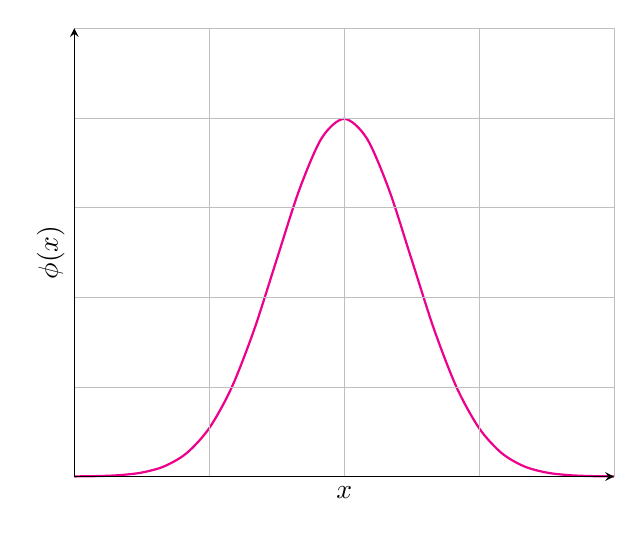
\begin{tikzpicture}
            \begin{axis}[
                xlabel=$x$,
                ylabel=$\phi(x)$,
                xmin=-4, xmax=4,
                ymin=0, ymax=0.5,
                axis lines=left,
                grid=both,
                grid style={line width=.1pt, draw=gray!10},
                major grid style={line width=.2pt,draw=gray!50},
                ticks=none,
                enlargelimits=false,
                clip=false,
                axis on top,
                every axis plot/.append style={thick},
            ]

            \addplot [magenta, smooth, domain=-4:4] {exp(-x^2 / 2) / sqrt(2*pi)};

            \end{axis}
            \end{tikzpicture}
            \item A continuous random variable is \textbf{normally distributed}, or has a \textbf{normal probability distribution}, if its relative frequency histogram has the shape of a normal curve.
            \item \textbf{Inflection Points:} On a bell shaped curve (normal curve), the graph has two inflection points. At $\mu \pm \sigma$, these points are where the graph shifts from increasing at an increasing rate, to increasing at a decreasing rate
            \item If a normal random variable X has a mean different from 0 or a standard deviation different from 1, we can transform X into a \textbf{standard normal random variable Z} whose mean is 0 and standard deviation is 1. 
            \item A \textbf{normal probability plot} is a graph that plots observed data versus normal scores. 
          \item A \textbf{normal score} is the expected z-score of the data value, assuming that the distribution of the random variable is normal. The expected z-score of an observed value depends on the number of observations in the data set.
                    \item The \textbf{sampling distribution} of a statistic is a probability distribution for all possible values of the statistic computed from a sample of size $n $
        \item The \textbf{sampling distribution of the sample mean} $\overline{x} $ is the probability distribution of all possible values of the random variable $\overline{x} $ computed from a sample of size $n$ from a population with mean $\mu $ and standard deviation $\sigma $.
        \item The standard deviation of the sampling distribution of $\overline{x} $, $\sigma_{\overline{x}} $, is called the \textbf{standard error} of the mean.
            \textbf{Note:} As the sample size $n $ increases, the standard error of the mean \textbf{decreases} 
        \item \textbf{The Central Limit Theorem:} Regardless of the shape of the underlying population, the sampling distribution of $\overline{x} $  becomes approximately normal as the sample size, $n $, increases
         \item \textbf{The sample proportion}, $\hat{p} $, is a statistic that estimates the population proportion, $p $.
    \end{itemize}

    \pagebreak 
    \phantomsection
    \addcontentsline{toc}{subsection}{5-8 Formulas}
    \subsection*{5-8 Formulas}
    \bigbreak \noindent 
        \begin{itemize}
        \item \textbf{Computing probability with the empirical method}
        \begin{align*}
            P(E) = \text{Relative frequency of E} = \frac{Frequency\ of\ E}{number\ of\ trials\ of\ experiment}
        .\end{align*}
      \item \textbf{Computing Probability With The Classical Method}
            \begin{itemize}
                \item If an experiment has n equally likely outcomes and if the number of ways that an event E can occur is m, then the probability of E,P(E), is
            \end{itemize}
            \begin{align*}
                P(E) = \frac{\text{number of ways that $E$ can occur}}{\text{number of possible outcomes}} = \frac{m}{n}
            .\end{align*}
            \begin{itemize}
                \item So, if S is the sample space of this experiment, then
                    \begin{align*}
                        P(E) = \frac{N(E)}{N(S)}
                    .\end{align*}
            where N(E) is the number of outcomes in E, and N(S) is the number of outcomes in the sample space.
            \end{itemize}
                    \item \textbf{Addition Rule for Disjoint Events:}
            \begin{itemize}
                \item if $E $ and $F $ are disjoint (or mutually exclusive) events, then:
                    \begin{align*}
                        P(E\ or\ F) = P(E) + P(F)
                    .\end{align*}
            \end{itemize}
        \item \textbf{Addition Rule for Non-Disjoint Events (General Addition Rule)}
          \begin{align*}
            P(E\ or\ F) = (P(E) + P(F)) - P(E\ and\ F)
          .\end{align*}
        \item \textbf{Complement Rule:}
            \begin{itemize}
                \item If $E$ represents any event and $E^{C}$ represents the complement of E, then
            \end{itemize}
            \begin{align*}
                P(E^{C}) = 1-P(E)                
            .\end{align*}
          \item \textbf{Multiplication Rule For Independent Events:}
    \begin{itemize}
      \item If $E_1, E_2, E_3, \ldots, E_n$ are independent events, then
    \end{itemize}
    \begin{align*}
         P(E_1 \text{ and } E_2 \text{ and } E_3 \text{ and } \ldots \text{ and } E_n) = P(E_1) \cdot P(E_2) \cdot \ldots \cdot P(E_n)
    .\end{align*}
            \item \textbf{Notation for probability of discrete random variables}
            \begin{align*}
                P(X)
            .\end{align*}
            \begin{itemize}
                \item Read as:
                    \begin{center}
                        "The probability that the random variable $X $ equals $x $"
                    \end{center}
            \end{itemize}
        \item \textbf{Mean of a Discrete Random Variable}
            \begin{align*}
                \mu_X = \summation{n}{i=1}\ \  x \cdot P(x)
            .\end{align*}
            Where $x $ is the value of the random variable and $P(x)$ is the probability of observing the value $x$.
        \item \textbf{Expected Value:}
            \begin{align*}
                E(X) = \mu_{X}
            .\end{align*}
        \item \textbf{Standard Deviation of a Discrete Random Variable}
            \begin{align*}
                \sigma_X = \sqrt{\sum [(x - \mu_X)^2 \cdot P(x)]}
            .\end{align*}
        Where $x$ is the value of the random variable, $\mu_X$ is the mean of the random variable, and $P(x)$ is the probability of observing $x$.
        \item \textbf{Variance of discrete random variable:}
            \begin{align*}
                \sigma^{2}
            .\end{align*}
          \item \textbf{nCk (Combinations):}
              \begin{itemize}
                  \item The  $n$  objects are distinct
                  \item Repetition of objects is not allowed, and
                  \item Order is not important
              \end{itemize}
              \begin{align*}
                  nCk = \frac{n!}{(k!(n-k)!)}
              .\end{align*}
            \item \textbf{Binomial Probability Distribution Function}
                \begin{align*}
                    P(x) = \binom{n}{x} \cdot p^x \cdot (1 - p)^{n-x}, \quad x = 0, 1, 2, \ldots, n
                .\end{align*}
                where $p$ is the probability of success.
            \item \textbf{Mean (or Expected Value) and Standard Deviation of a Binomial Random Variable}
                \begin{itemize}
                    \item A binomial experiment with n independent trials and probability of success p has mean, $\mu_X$, and standard deviation, $\sigma_X$, given by the formulas
                \end{itemize}
                \begin{align*}
                    \mu_X = np,\ \text{and standard deviation,}\ \sigma_X = \sqrt{np(1-p)}
                .\end{align*}
              \item \textbf{Drawing normal probability plot by hand}
                \begin{align*}
                  f_{i} = \frac{i - 0.375}{n + 0.25}
                .\end{align*}
                Then use table to find expected zscores
                        \item \textbf{Mean of sampling distribution}
            \begin{align*}
                \mu_{\overline{x}} = \mu
            .\end{align*}
        \item \textbf{Standard Deviation of sampling distribution}
            \begin{align*}
                \sigma_{\overline{x}} = \sqrt{\frac{N-n}{N-1}} \cdot \frac{\sigma}{\sqrt{n}}
            .\end{align*}
        \item \textbf{finite population correction factor}
            \begin{align*}
                \sqrt{\frac{N-n}{N-1}}
            .\end{align*}
                     \item Suppose that a random sample of size n is obtained from a population in which each individual either does or does not have a certain characteristic. The \textbf{sample proportion}, denoted $\hat{p}$ (read “p-hat”), is given by:
             \begin{align*}
                 \hat{p} = \frac{x}{n}
             .\end{align*}
            where $x $ is the number of individuals in the sample with the specified characteristic. 
        \item \textbf{Mean of sampling distribution}
            \begin{align*}
                \mu_{\hat{p}} = p
            .\end{align*}
        \item \textbf{Standard Deviation of the sampling distribution:}
            \begin{align*}
               \sigma_{\hat{p}} = \sqrt{\frac{p(1-p)}{n}} 
            .\end{align*}     
    \end{itemize}


    \pagebreak 
    \begin{center}
      \phantomsection
      \addcontentsline{toc}{subsection}{5-8 Concepts:}
      \subsection*{5-8 Concepts:}
    \end{center}
    \line(1,0){490}
    \bigbreak \noindent
    \phantomsection
    \addcontentsline{toc}{subsection}{Rules of Probability}
    \subsection*{Rules of Probability}
    \bigbreak \noindent 
    \textbf{Rules of Probability:}
      \begin{enumerate}
        \item The probability of any event E, $P(E)$, must be greater than or equal to 0 and less than or equal to 1. That is, $0 \leq P(E) \leq 1$.
        \item The sum of the probabilities of all outcomes must equal 1. That is, if the sample space $S = \{e_1, e_2, \dots, e_n\}$, then
            \begin{align*}
                P(e_1) + P(e_2) + \dots + P(e_n) = 1.
            .\end{align*}
    \end{enumerate}
    \bigbreak \noindent 
    Consider The Table:
    \bigbreak \noindent 
        \begin{center}
              \begin{tabular}{|l|c|}
              \hline
              Color & Probability \\
              	\hline
               	 Brown  & 0.12  \\
              	\hline
              	 Yellow & 0.15 \\
              	 \hline 
              	 Red & 0.12 \\
              	 \hline
              	 Blue & 0.23 \\
              	 \hline
              	 Orange & 0.23 \\
              	 \hline
              	 Green & 0.15 \\
              	 \hline
              \end{tabular}
          \end{center}
      \bigbreak \noindent 
      \textbf{Does this satisfy the rules?}
      \bigbreak \noindent 
      Rule 1 is satisfied because all probabilities are between 0 and 1, inclusive.
      \bigbreak \noindent 
      Rule 2 is satisfied because $\sum P(E)= 1$

      \bigbreak \noindent \bigbreak \noindent 
      \phantomsection
      \addcontentsline{toc}{subsection}{Unusual Event}
      \subsection*{Unusual Event}
    \bigbreak \noindent 
    Typically, an event with a probability less than 0.05 (or 5\%) is considered unusual, but this cutoff point is not set in stone. The researcher and the context of the problem determine the probability that separates unusual events from not so unusual events.
    \bigbreak \noindent 
    \phantomsection
    \addcontentsline{toc}{subsection}{The three methods for determining the probability of an event:}
    \subsection*{The three methods for determining the probability of an event:}
    \bigbreak \noindent 
    \begin{itemize}
        \item the Empirical Method
        \item the Classical Method
        \item the Subjective Method
    \end{itemize}
    \pagebreak


    \bigbreak \noindent \bigbreak \noindent 
    \phantomsection
    \addcontentsline{toc}{subsection}{Rule for claiming Independence:}
    \subsection*{Rule for claiming Independence:}
    \bigbreak \noindent 
    When we take small samples from large finite populations, we make the assumption of independence even though the events are technically dependent.
    \bigbreak \noindent 
    As a general rule of thumb, if the sample size $n $ is no more than 5\% of the population $N $ ($n \leq 0.05 N $), we assume independence.

    \bigbreak \noindent \bigbreak \noindent 
    \phantomsection
    \addcontentsline{toc}{subsection}{Compute "at-least" Probabilities:}
    \subsection*{Compute "at-least" Probabilities:}
    \bigbreak \noindent 
      Usually, when computing probabilities involving the phrase at least, use the Complement Rule.
    \bigbreak \noindent 
    The phrase at least means “greater than or equal to.” For example, a person must be at least 17 years old to see an R-rated movie. This means that the person's age must be greater than or equal to 17 to watch the movie.

    \bigbreak \noindent \bigbreak \noindent 
    \phantomsection
    \addcontentsline{toc}{subsection}{Poll Indicates Different from our assumptions}
    \subsection*{Poll Indicates Different from our assumptions}
    \bigbreak \noindent 
    Consider the following scenario:
    \bigbreak \noindent 
    \textit{According to a​ poll, about ​17\% of adults in a country bet on professional sports. Data indicates that ​47.3\% of the adult population in this country is male. Assuming that betting is independent of​ gender, compute the probability that an adult from this country selected at random is a male and bets on professional sports.}
    \bigbreak \noindent 
      \textbf{Solution:}
      \bigbreak \noindent 
      \begin{align*}
        P(Male\ or\ Bet\ on\ Sports) = .17 \cdot .473 \\
        = .0804
      .\end{align*}
      \bigbreak \noindent 
      Now Consider:
      \bigbreak \noindent 
      \textit{The poll data indicated that ​\% of adults in this country are males and bet on professional sports. }
      \bigbreak \noindent 
      \textbf{Solution:}
      \bigbreak \noindent 
      The assumption was incorrect and the events are \textbf{not independent}.
      
      \bigbreak \noindent \bigbreak \noindent 
      \phantomsection
      \addcontentsline{toc}{subsection}{Rules for a Discrete Probability Distribution:}
      \subsection*{Rules for a Discrete Probability Distribution:}
      \bigbreak \noindent 
      Let $P(x)$ denote the probability that the random variable $X$ equals $x$; then
      \begin{itemize}
          \item $ \sum P(x) = 1 $
          \item $0 \leq P(x) \leq 1$
      \end{itemize}

      \pagebreak 
      \phantomsection
      \addcontentsline{toc}{subsection}{Graph Discrete Probability Distributions}
      \subsection*{Graph Discrete Probability Distributions}
        \bigbreak \noindent 
      In the graph of a discrete probability distribution, the horizontal axis is the value of the discrete random variable and the vertical axis is the corresponding probability of the discrete random variable. When graphing a discrete probability distribution, we want to emphasize that the data are discrete. Therefore, draw the graph of discrete probability distributions using vertical lines above each value of the random variable to a height that is the probability of the random variable.
      \bigbreak \noindent 
      \begin{figure}[ht]
          \centering
          \incfig{enumac}
          \label{fig:enumac}
      \end{figure}

      \bigbreak \noindent \bigbreak \noindent 
      \phantomsection
      \addcontentsline{toc}{subsection}{Finding Mean of a Discrete Random Variable In Statcrunch:}
      \subsection*{Finding Mean of a Discrete Random Variable In Statcrunch:}
      \bigbreak \noindent 
      \begin{enumerate}
          \item Stat $> $ Calculators $> $ Custom
          \item Select Values in:
          \item Select Weights in (P(X)):
          \item Compute
      \end{enumerate}

      \bigbreak \noindent \bigbreak \noindent 
      \phantomsection
      \addcontentsline{toc}{subsection}{How to Interpret the Mean of a Discrete Random Variable}
      \subsection*{How to Interpret the Mean of a Discrete Random Variable}
      \bigbreak \noindent 
        The mean of a discrete random variable can be thought of as the mean outcome of the probability experiment if we repeated the experiment many times. 
      \bigbreak \noindent 
      As the number of repetitions of the experiment increases... The mean value of the $n $ trials will approach $\mu_{X}$ (The difference between $\overline{x} $ and $\mu_{X} $ gets closer to 0 as $n$ increases)

      \pagebreak 
      \phantomsection
      \addcontentsline{toc}{subsection}{Life insurance policy example (expected value)}
      \subsection*{Life insurance policy example (expected value)}
      \bigbreak \noindent 
      \begin{mdframed}
      \textbf{Example: A term life insurance policy will pay a beneficiary a certain sum of money upon the death of the policy holder. These policies have premiums that must be paid annually. Suppose a life insurance company sells a \$250,000 one-year term life insurance policy to a 49-year-old female for \$530. According to the National Vital Statistics Report, Vol. 47, No. 28, the probability that the female will survive the year is 0.99791. Compute the expected value of this policy to the insurance company.}
      \bigbreak \noindent 
      \textbf{Approach:}
      \bigbreak \noindent 
      The experiment has two possible outcomes: survival or death. Let the random variable X represent the payout (money lost or gained), depending on survival or death of the insured. Assign probabilities to each payout and substitute these values into $\mu_{X} = \sum (x \cdot P(X)) $
      \bigbreak \noindent 
      \textbf{Step 1}. Because $P(\text{survives}) = 0.99791$, $P(\text{dies}) = 0.00209$. If the client survives the year, the insurance company makes \$530, or $x = +530$. If the client dies during the year, the insurance company must pay \$250,000 to the client's beneficiary, but still keeps the \$530 premium; so $x = \$530 - \$250,000 = -\$249,470$. The value is negative because it is money paid by the insurance company. The probability distribution is listed in Table 3.
      \begin{center}
          \begin{center}
              \begin{tabular}{|l|c|}
              \hline
              $x$ & $ P(X)$ \\
              	\hline
               	\$530 (survives)  & 0.99791  \\
              	\hline
              	-\$249,470 (dies) &0.00209 \\
              	\hline
              \end{tabular}
          \end{center}
      \end{center}
      \bigbreak \noindent 
      \textbf{Step 2.} The expected value (from the point of view of the insurance company) of the policy is
      \begin{align*}
          E(X) = \mu_{X} \\
          = \sum (x \cdot P(X)) \\
          = (\$530 \cdot 0.99791) + (-\$249470 \cdot 0.00209) \\
          = \$7.50
      .\end{align*}
      \bigbreak \noindent 
      \textbf{Therefore:}
      \bigbreak \noindent 
      The company expects to make \$7.50 for each 49-year-old female client it insures. The \$7.50 profit of the insurance company is a long-term result. It does not make \$7.50 on each 49-year-old female it insures; rather, the average profit per 49-year-old female insured is \$7.50. Because this is a long-term result, the insurance "idea" will not work with only a few insured.
    \end{mdframed}

    \pagebreak 
    \phantomsection
    \addcontentsline{toc}{subsection}{Standard Deviation of a Random Discrete Variable In Statrunch}
    \subsection*{Standard Deviation of a Random Discrete Variable In Statrunch}
    \bigbreak \noindent 
      \textbf{Statcrunch Steps:}
      \begin{enumerate}
          \item Stat $> $ Calculators $> $ Custom
        \item Select Values in:
        \item Select Weights in (P(X)):
        \item Compute
      \end{enumerate}

      \bigbreak \noindent 
      \phantomsection
      \addcontentsline{toc}{subsection}{Criteria for a Binomial Probability Experiment}
      \subsection*{Criteria for a Binomial Probability Experiment}
      \bigbreak \noindent 
        An experiment is said to be a \textbf{binomial experiment} if:
      \begin{enumerate}
          \item The experiment is preformed a fixed number of times. Each repetition of the experiment is called a \textbf{trial}
            \item The trials are independent. This means that the outcome of one trial will not affect the outcome of the other trials.
            \item for each trial, there are two mutually exclusive outcomes, success or failure.
            \item The probability of success is fixed for each trial of the experiment.
      \end{enumerate}

      \bigbreak \noindent \bigbreak \noindent 
      \phantomsection
      \addcontentsline{toc}{subsection}{Notation used in the binomial probability distribution:}
      \subsection*{Notation used in the binomial probability distribution:}
      \bigbreak \noindent 
      \begin{itemize}
          \item There are $n $ independent trials of the experiment.
        \item let $p $ denote the probability of success so that $1-p $ is the probability of failure
        \item Let $X $ be a binomial random variable that denotes the number of successes in $n $ independent trials of the experiment. So $0 \leq X \leq n $
      \end{itemize}

      \bigbreak \noindent \bigbreak \noindent 
      \phantomsection
      \addcontentsline{toc}{subsection}{three methods for obtaining binomial probabilities:}
      \subsection*{three methods for obtaining binomial probabilities:}
      \bigbreak \noindent 
            \begin{enumerate}
          \item The binomial probability distribution formula
          \item A table of binomial probabilities
          \item Technology
      \end{enumerate}

      \pagebreak 
      \phantomsection
      \addcontentsline{toc}{subsection}{Using the Binomial Probability Distribution Function in Statcrunch}
      \subsection*{Using the Binomial Probability Distribution Function in Statcrunch}
      \bigbreak \noindent 
            \textbf{Steps:}
      \begin{enumerate}
          \item Stat $> $ Calculators $> $ Binomial
        \item Enter $n $
        \item Enter $p $
        \item Enter info for $P(X)$
        \item Compute
      \end{enumerate}

      \bigbreak \noindent \bigbreak \noindent 
      \phantomsection
      \addcontentsline{toc}{subsection}{Shape of Binomial Probability Distribution for Various Values of p}
      \subsection*{Shape of Binomial Probability Distribution for Various Values of p }
      \bigbreak \noindent 
      The binomial probability distribution is
      \begin{itemize}
          \item skewed right if $p <0.5$
          \item symmetric and approximately bell-shaped if $p=0.5$
          \item skewed left of $p>0.5$ 
      \end{itemize}

      \bigbreak \noindent \bigbreak \noindent 
      \phantomsection
      \addcontentsline{toc}{subsection}{Shape of the Graph of a Binomial Probability Distribution for Various Values of n}
      \subsection*{Shape of the Graph of a Binomial Probability Distribution for Various Values of n}
      \bigbreak \noindent 
            \begin{itemize}
          \item For a fixed $p$, as the number of trials $n $ in a binomial experiment increases, the probability distribution of the random variable $X$ becomes bell-shaped.
          \item As a rule of thumb, if $np(1-p) \geq 10$, the probability distribution will be approximately bell-shaped.
      \end{itemize}
      \bigbreak \noindent 
      \nt{This result allows us to use the Empirical Rule to identify unusual observations in a binomial experiment. Recall that the Empirical Rule states that in a bell-shaped distribution, about 95\% of all observations lie within 2 standard deviations of the mean. That is, about 95\% of the observations lie between μ−2σ and μ+2σ. Any observation that lies outside this interval may be considered unusual because the observation occurs less than 5\% of the time.}

      \pagebreak \bigbreak \noindent 
          \begin{mdframed}
        \textbf{Example: According to CTIA, 55\% of all U.S. households are wireless-only. In a simple random sample of 500 households, 301 were wireless-only. Is this result unusual?}
        \bigbreak \noindent 
        \textbf{Approach:}
        \bigbreak \noindent 
        Because $np(1-p) = 500(0.55)(1-0.55) = 123.75 \geq 10$, the binomial probability distribution is approximately bell-shaped. Therefore, we can use the Empirical Rule: If the observation is less than $\mu - 2\sigma$ or greater than $\mu + 2\sigma$, it is unusual.
        \bigbreak \noindent 
        \textbf{Solution:}
        We have $\mu_X = 500(0.55) = 275$ and $\sigma_X = \sqrt{np(1-p)} = \sqrt{500(0.55)(1-0.55)} = 11.1$. Now,
        \begin{align*}
            \mu_X - 2\sigma_X = 275 - 2(11.1) = 275 - 22.2 = 252.8\\ and\\ \mu_X + 2\sigma_X = 275 + 2(11.1) = 275 + 22.2 = 297.2.
        .\end{align*}
        \bigbreak \noindent 
        Any value less than 252.8 or greater than 297.2 is unusual; therefore, 301 is an unusual result. We should try to identify the reason for its value. Perhaps the percentage of households that are wireless-only has increased.
      \end{mdframed}

      \bigbreak \noindent \bigbreak \noindent 
      \phantomsection
      \addcontentsline{toc}{subsection}{Probability Density Function (pdf) Rules:}
      \subsection*{Probability Density Function (pdf) Rules:}
      \bigbreak \noindent 
        \begin{enumerate}
          \item The total area under the graph of the equation over all possible values of the random variable must equal 1
          \item The height of the graph of the equation must be greater than or equal to 0 for all possible values of the random variable. That is, the graph of the equation must lie on or above the horizontal axis for all possible values of the random variable.
        \end{enumerate}

      \pagebreak 
      \phantomsection
      \addcontentsline{toc}{subsection}{Area as a Probability:}
      \subsection*{Area as a Probability:}
      \bigbreak \noindent 
      The probability of choosing a time that is between 15 and 30 seconds after the minute is the area under the uniform density function.
      \bigbreak \noindent 
      \begin{figure}[ht]
          \centering
          \incfig{figaro3}
          \label{fig:figaro3}
      \end{figure}

      \bigbreak \noindent \bigbreak \noindent 
      \phantomsection
      \addcontentsline{toc}{subsection}{Effects of mean and standard deviation on normal curve}
      \subsection*{Effects of mean and standard deviation on normal curve}
      \bigbreak \noindent 
      \begin{itemize}
        \item as the mean increases, the graph slides to the right
        \item as the mean decreases, the graph slides to the left
        \item as the standard deviation increases, the graph flattens out and becomes wider 
        \item as the standard deviation decreases, the graph compresses out and becomes steeper 
      \end{itemize}

      \phantomsection
      \addcontentsline{toc}{subsection}{Properties of the Normal Curve}
      \subsection*{Properties of the Normal Curve}
      \bigbreak \noindent 
          The normal probability density function satisfies all the requirements of probability distributions. Now we list the properties of the normal density curve. The video explains the properties.
    \begin{enumerate}
    \item Because mean = median = mode, the normal curve has a single peak and the highest point occurs at $x=\mu$.
    \item The normal curve has inflection points at $\mu-\sigma$ and $\mu+\sigma$.
    \item The area under the normal curve is 1.
    \item The area under the normal curve to the right of $\mu$ equals the area under the normal curve to the left of $\mu$, which equals 0.5.
    \item As $x$ increases without bound (gets larger and larger), the graph approaches, but never reaches, the horizontal axis. As $x$ decreases without bound (gets more and more negative), the graph approaches, but never reaches, the horizontal axis.
    \item The Empirical Rule:
    \begin{itemize}
        \item Approximately 68\% of the area under the normal curve is between $x=\mu-\sigma$ and $x=\mu+\sigma$.
        \item Approximately 95\% of the area is between $x=\mu-2\sigma$ and $x=\mu+2\sigma$.
        \item Approximately 99.7\% of the area is between $x=\mu-3\sigma$ and $x=\mu+3\sigma$.
    \end{itemize}
    \end{enumerate}

    \pagebreak 
    \phantomsection
    \addcontentsline{toc}{subsection}{The Role of Area in the Normal Density Function:}
    \subsection*{The Role of Area in the Normal Density Function:}
    \bigbreak \noindent 
        \bigbreak \noindent 
    Suppose that a random variable $X$ is normally distributed with mean $\mu$ and standard deviation $\sigma$. The area under the normal curve for any interval of values of the random variable $X$ represents either
    \bigbreak \noindent 
    \begin{itemize}
        \item The proportion of the population with the characteristic described by the interval of values,
        \smallbreak
        or
        \item The probability that a randomly selected individual from the population will have the characteristic described by the interval of values.
    \end{itemize}

    \bigbreak \noindent \bigbreak \noindent 
    \phantomsection
    \addcontentsline{toc}{subsection}{Find and Interpret the Area under a Normal Curve}
    \subsection*{Find and Interpret the Area under a Normal Curve}
    \bigbreak \noindent 
    We use z-scores to find the area under a normal curve by hand. Recall that the z-score allows us to transform a random variable X with mean $\mu$ and standard deviation $\sigma $ into a random variable Z with mean 0 and standard deviation 1.

    \pagebreak 
    \phantomsection
    \addcontentsline{toc}{subsection}{Standardizing a Normal Random Variable:}
    \subsection*{Standardizing a Normal Random Variable:}
    \bigbreak \noindent 
        Suppose that the random variable $X$ is normally distributed with mean $\mu$ and standard deviation $\sigma$.
    \bigbreak \noindent 
    Then the random variable 
    \begin{align*}
        Z = \frac{X - \mu}{\sigma}
    .\end{align*}
    is normally distributed with mean $\mu = 0$ and standard deviation $\sigma = 1$.
    \bigbreak \noindent 
    The random variable $Z$ is said to have the \textbf{standard normal distribution.}
        \bigbreak \noindent 
    Consider an example:
    \bigbreak \noindent 
    IQ scores can be modeled by a normal distribution with $\mu = 100 $ and $\sigma = 15$ Suppose a person has an IQ of 120
    \bigbreak \noindent 
    \textit{Figure:}
    \bigbreak \noindent 
    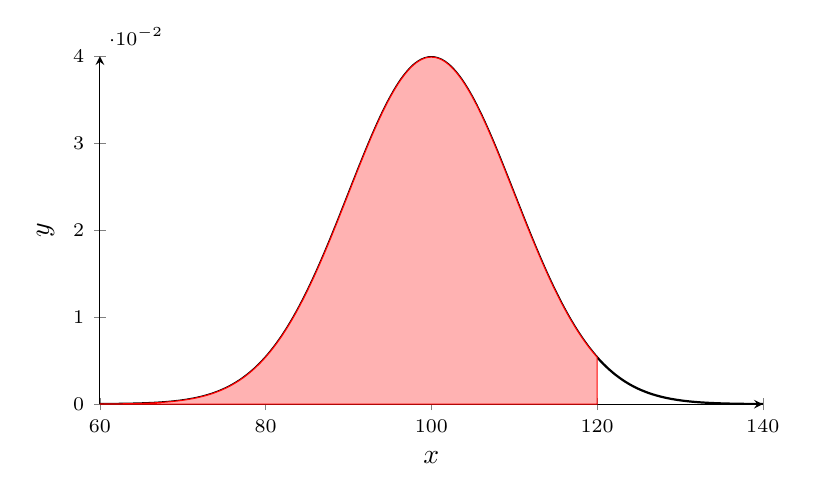
\begin{tikzpicture}
      \begin{axis}[
        width=10cm,
        height=6cm,
        axis lines=left,
        xlabel=$x$,
        ylabel=$y$,
        xmin=60,
        xmax=140,
        ymin=0,
        ymax=0.04,
        xtick={60,80,100,120,140},
        % ytick={0,0.01,0.02,0.03,0.04},
        % yticklabels={0,0.01,0.02,0.03,0.04},
        tick label style={font=\scriptsize},
        samples=100,
        smooth,
        domain=60:140,
      ]
      
      % Bell-shaped curve
      \addplot[black, fill=none, thick] {exp(-((x-100)^2)/(2*10^2))/(10*sqrt(2*pi))};
      
      % Red shaded area
      \addplot[red, fill=red!30, domain=60:120] {exp(-((x-100)^2)/(2*10^2))/(10*sqrt(2*pi))} \closedcycle;
      \end{axis}
    \end{tikzpicture}
    \bigbreak \noindent 
        Now we can transform this into a standard normal (Z distribution)
        \begin{align*}
            Z = \frac{120-100}{15} \\
            = 1.33
        .\end{align*}
        \bigbreak \noindent 
        \textit{Figure:}
        \bigbreak \noindent 
        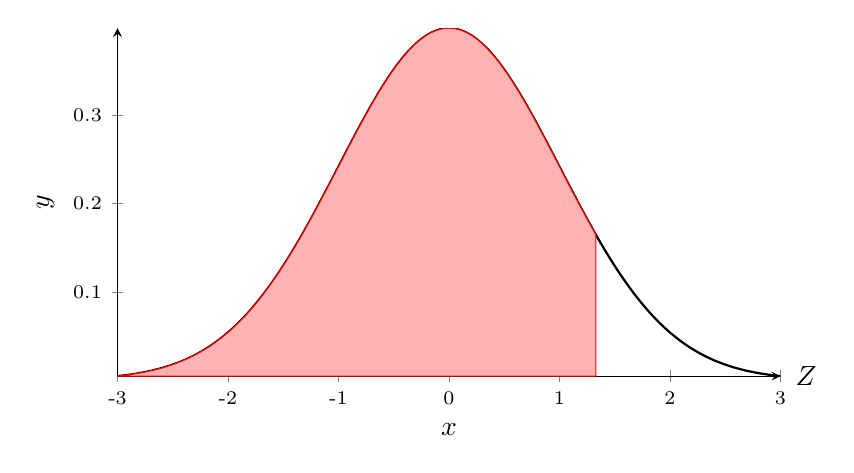
\begin{tikzpicture}
      \begin{axis}[
        width=10cm,
        height=6cm,
        axis lines=left,
        xlabel=$x$,
        ylabel=$y$,
        xtick={-3, -2, -1, 0, 1, 2, 3},
        xticklabels={-3, -2, -1, 0, 1, 2, 3},
        % ytick={0, 0.2, 0.4, 0.6, 0.8, 1.0},
        % yticklabels={0, 0.2, 0.4, 0.6, 0.8, 1.0},
        tick label style={font=\scriptsize},
        samples=100,
        smooth,
        domain=-3:3,
      ]
      
      % Bell-shaped curve
      \addplot[black, fill=none, thick] {exp(-x^2/2)/(sqrt(2*pi))};
      
      % Red shaded area
      \addplot[red, fill=red!30, domain=-3:1.33] {exp(-x^2/2)/(sqrt(2*pi))} \closedcycle;
      
      \end{axis}
      \node[anchor=east] at (9,0) {$Z$};
    \end{tikzpicture}
    \bigbreak \noindent 
    Then by looking at the Table, we can determine the area in the red shaded region. Which is .9082. From this we can also determine that the area in the red region of our original distribution is also .9082
    \bigbreak \noindent 
    If we wanted to find the area of the unshaded region, we can use the complement rule
    \begin{align*}
      1- .9082 \\
      = .0918
    .\end{align*}
    \bigbreak \noindent 
    \textbf{Percentiles:}
    \bigbreak \noindent 
    Because the area under the normal curve represents a proportion, we can also use the area to find percentile ranks of scores. 
    \bigbreak \noindent 
    So we can say that 90.82\% have an IQ $ \leq 120$

  \bigbreak \noindent \bigbreak \noindent 
  \phantomsection
  \addcontentsline{toc}{subsection}{Finding an interpreting Area under a Normal Curve With Statcrunch:}
  \subsection*{Finding an interpreting Area under a Normal Curve With Statcrunch:}
      \bigbreak \noindent \bigbreak \noindent 
    \begin{enumerate}
        \item Stat $> $ Calculators $> $ Normal 
        \item Input Mean
        \item Input Standard Deviation
        \item Input X
        \item Compute
    \end{enumerate}

    \bigbreak \noindent 
    \phantomsection
    \addcontentsline{toc}{subsection}{Find the Value of a Normal Random Variable:}
    \subsection*{Find the Value of a Normal Random Variable:}
    \bigbreak \noindent 
    Often, we do not want to find the proportion, probability, or percentile given a value of a normal random variable. Rather, we want to find the value of a normal random variable that corresponds to a certain proportion, probability, or percentile. For example, we might want to know the height of a 3-year-old girl who is at the 20th percentile. Or we might want to know the scores on a standardized exam that separate the middle 90\% of scores from the bottom and top 5\%.
    \bigbreak \noindent 
    \begin{mdframed}
        \textbf{Example: The heights of a pediatrician's 3-year-old females are approximately normally distributed, with mean 38.72 inches and standard deviation 3.17 inches. Find the height of a 3-year-old female at the $20^{th} $ percentile.}
        \bigbreak \noindent 
        \textbf{Approach:}
        \bigbreak \noindent 
        Use .2 in Statcrunch steps mentioned previously as what P(X) is equal to.
    \end{mdframed}
    \begin{mdframed}
        \textbf{Example: The mean incubation time of fertilized eggs is  days. Suppose the incubation times are approximately normally distributed with a standard deviation of  day. Determine the incubation times that make up the middle 97\%}
        \bigbreak \noindent 
        \textbf{Solution:}
        \bigbreak \noindent 
        So in statcrunch, we will use values 0.05, and 0.97
    \end{mdframed}


  \pagebreak 
  \phantomsection
  \addcontentsline{toc}{subsection}{Important Notation for the Future}
  \subsection*{Important Notation for the Future}
  \bigbreak \noindent 
  The notation $z_{\alpha}$ (pronounced "z sub alpha") is the z-score such that the area under the standard normal curve to the right of $z_{\alpha}$ is $\alpha$. 
  \bigbreak \noindent 
  \begin{mdframed}
    \textbf{Example: Find the value of $Z_{0.21} $}
    \bigbreak \noindent 
    \textbf{Solution:}
    So we want to find the area to the right of 0.21, in statcrunch:
    \begin{enumerate}
      \item Stat $> $ Calculator $> $ Normal
      \item Mean: 0 
      \item Std. Dev: 1
      \item $P(x \geq 0) = 0.21$
      \item Compute!
    \end{enumerate}
  \end{mdframed}

  \bigbreak \noindent \bigbreak \noindent 
  \phantomsection
  \addcontentsline{toc}{subsection}{Drawing a Normal Probability Plot Using Statcrunch (Also shows correlation)}
  \subsection*{Drawing a Normal Probability Plot Using Statcrunch}
    \bigbreak \noindent 
    \begin{enumerate}
        \item Graph $> $ QQ plot
        \item Select Column
        \item Select Correlation Statistic
        \item Compute
    \end{enumerate}
    \bigbreak \noindent 
    \nt{Normal probability plot is observed values as x and expected z-scores as y}
    \bigbreak \noindent 

    \pagebreak 
    \phantomsection
    \addcontentsline{toc}{subsection}{A Rule of Thumb for Invoking the Central Limit Theorem:}
    \subsection*{A Rule of Thumb for Invoking the Central Limit Theorem:}
    \bigbreak \noindent 
         \begin{enumerate}
         \item The shape of the distribution of the population from which the sample is drawn dictates the size of the sample required for the distribution of the sample mean to be normal.
         \item The more skewed the distribution of the population is, the larger the sample size needed to invoke the Central Limit Theorem.
        \item \textbf{If the distribution of the population is unknown or not normal, then the distribution of the sample mean is approximately normal provided that the sample size is greater than or equal to 30.}
     \end{enumerate}

     \bigbreak \noindent \bigbreak \noindent 
     \phantomsection
     \addcontentsline{toc}{subsection}{cutting the standard error of the mean in​ half}
     \subsection*{cutting the standard error of the mean in​ half}
     \bigbreak \noindent 
     The sample size must be increased by a factor of four to cut the standard error in half.


     \smallbreak
     \phantomsection
     \addcontentsline{toc}{subsection}{​(a) Suppose a simple random sample of size n is obtained from a population whose distribution is skewed right. As the sample size n​ increases, what happens to the shape of the distribution of the sample​ mean?}
     \subsection*{Suppose a simple random sample of size n is obtained from a population whose distribution is skewed right. As the sample size n increases, what happens to the shape of the distribution of the sample mean?}
     \bigbreak \noindent 
     \textbf{Answer:} The distribution becomes approximately normal.
     \bigbreak \noindent 
     \textbf{​(b) For the three probability distributions​ shown, rank each distribution from lowest to highest in terms of the sample size required for the distribution of the sample mean to be approximately normally distributed. }
     \begin{enumerate}
       \item \textbf{Uniform}: Lowest
        \item \textbf{Normal}: Medium
        \item \textbf{Skewed}: Highest
     \end{enumerate}

     \bigbreak \noindent \bigbreak \noindent 
     \phantomsection
     \addcontentsline{toc}{subsection}{Sampling Distribution of phat}
     \subsection*{Sampling Distribution of phat}
     \bigbreak \noindent 
             For a simple random sample of size $n$ with a population proportion $p$, 
        \begin{itemize}
            \item The shape of the sampling distribution of $\hat{p}$ is approximately normal provided $np(1-p) \geq 10$.
            \item The mean of the sampling distribution of $\hat{p}$ is:
                \begin{align*}
                    \mu_{\hat{p}} = p.
                .\end{align*}
            \item The standard deviation of the sampling distribution of $\hat{p}$ is:
                \begin{align*}
                    \sigma_{\hat{p}} = \sqrt{\frac{p(1-p)}{n}}
                .\end{align*}
        \end{itemize}
        \bigbreak \noindent 
        \nt{The sample size, $n$, can be no more than 5\% of the population size, $N$. That is, $n \leq 0.05N$.}

        \pagebreak 
        \phantomsection
        \addcontentsline{toc}{subsection}{9-12 Subsection Titles}
        \subsection*{9-12 Subsection Titles}
        \bigbreak \noindent 
        \textbf{Chapter 9:}
        \begin{itemize}
          \item 9.1: Estimating a Population Proportion
          \item 9.2: Estimating a Population Mean
          \item 9.3: Putting It Together: Which Procedure Do I Use?
        \end{itemize}
        \bigbreak \noindent 
        \textbf{Chapter 10:}
        \begin{itemize}
          \item 10.1: The Language of Hypothesis Testing
          \item 10.2A: Hypothesis Tests on a Population Proportion with Simulation
          \item 10.2B: Hypothesis Tests on a Population Proportion Using the Normal Model
          \item 10.3: Hypothesis Tests for a Population Mean
          \item 10.4: Putting It Together: Which Procedure Do I Use?
        \end{itemize}
        \bigbreak \noindent 
        \textbf{Chapter 11:}
        \begin{itemize}
          \item 11.1A: Using Randomization Techniques to Compare Two Proportions
          \item 11.1: Inference about Two Population Proportions: Independent Samples
          \item 11.2: Inference about Two Population Means: Dependent Samples
          \item 11.3A Using Randomization Techniques to Compare Two Independent Means
          \item 11.3 Inference about Two Population Means: Independent Samples
          \item 11.4: Putting It Together: Which Procedure Do I Use?
        \end{itemize}
        \bigbreak \noindent 
        \textbf{Chapter 12:}
        \begin{itemize}
          \item 12.1 Goodness-of-Fit Test
          \item 12.2 Tests for Independence and the Homogeneity of Proportions
        \end{itemize}

        \pagebreak 
        \phantomsection
      \addcontentsline{toc}{subsection}{9-12 Vocab}
        \subsection*{9-12 Vocab}
        \begin{itemize}
          \item A \textbf{point estimate} is the value of a statistic that estimates the value of a parameter.
          \item \textbf{A Confidence Interval} for an  unknown parameter consists of an interval of numbers based on a point estimate.
          \item \textbf{The level of confidence} represents the expected proportion of intervals that will contain the parameter if a large number of different samples is obtained.
          \item \textbf{Critical Value} represents the number of standard deviations the sample statistic can be from the parameter and still result in an interval that includes the parameter.
          \item \textbf{The point estimate of the population mean}, $\mu$, is the sample mean, $\overline{x}$.
          \item \textbf{T-Interval:} confidence interval that uses the t-distribution
          \item A \textbf{Hypothesis} is a statement regarding a characteristic of one or more populations
          \item \textbf{Hypothesis Testing} is used to test statements regarding a characteristic of one or more populations
          \textbf{Note:} The "heart" of hypothesis testing is making an assumption about reality, and collecting sample evidence to determine whether it contradicts the assumption.
          \item \textbf{Null Hypothesis} is a statement to be tested. The null hypothesis is a statement of no change, no effect or no difference and is assumed true until evidence indicates otherwise
          \item \textbf{alternative Hypothesis} is a statement that we are trying to find evidence to support
          \item Left- and right-tailed tests are referred to as \textbf{one-tailed tests}. 
          \item Reject the null hypothesis when the null hypothesis is true. This decision would be incorrect. This type of error is called a \textbf{Type I error.}
          \item Do not reject the null hypothesis when the alternative hypothesis is true. This decision would be incorrect. This type of error is called a \textbf{Type II error.}
          \item \textbf{level of significance.} is the probability of making a type-1 error
          \item When observed results are unlikely under the assumption that the null hypothesis is true, the result is \textbf{statistically significant} and we reject the statement in the null hypothesis.
          \item A model that generates data randomly under the assumption the statement in the null hypothesis is true. Call this model the \textbf{null model}. 
          \item A \textbf{P-value} is the probability of observing a sample statistic as extreme or more extreme than the one observed under the assumption that the statement in the null hypothesis is true. Put another way, the P-value is the likelihood or probability that a sample statistic will result in a statistic such as the one obtained if the statement in the null hypothesis is true.
          \item \textbf{Practical significance} refers to the idea that although small differences between the statistic and parameter stated in the null hypothesis are statistically significant, the difference may not be large enough to cause concern or be considered important. 
          \item A sampling method is \textbf{independent} when an individual selected for one sample does not dictate which individual is to be in the second sample.
          \item A sampling method is \textbf{dependent} when the individuals selected to be in one sample are used to determine the individuals in the second sample. (matched pairs samples)
        \item A \textbf{goodness-of-fit} test is an inferential procedure used to determine whether a frequency distribution follows a specific distribution.
        \item The \textbf{chi-square test for independence} is used to determine whether there is an association between a row variable and a column variable in a contingency table constructed from sample data.
            \begin{itemize}
                \item The null hypothesis is that the variables are not associated, or independent.
                \item The alternative hypothesis is that the variables are associated, or dependent.

            \end{itemize}
        \item In a \textbf{chi-square test for homogeneity of proportions}, we test whether different populations have the same proportion of individuals with some characteristic.

        \end{itemize}
        \bigbreak \noindent 

        \pagebreak 
        \phantomsection
        \addcontentsline{toc}{subsection}{9-12 Notation/Formulas}
        \subsection*{9-12 Notation/Formulas}
        \begin{itemize}
                  \item \textbf{Point Estimate for a Sample Proportion}
            \begin{align*}
                \hat{p} = \frac{x}{n}
            .\end{align*}
        \item The \textbf{Margin of Error} is denoted:
            \begin{align*}
                E 
            .\end{align*}
        \item \textbf{Confidence Intervals for a Proportion} are of the form:
            \begin{center}
                point estimate $\pm $ margin of error
            \end{center}
            That is:
            \begin{align*}
               \hat{p} \pm E 
            .\end{align*}
            We have 95\% confidence that the sampling proportion will lie between:
            \begin{align*}
                \hat{p} \pm 1.96 \sigma_{\hat{p}}  
            .\end{align*}
        \item \textbf{The level of confidence} is denoted:
            \begin{align*}
                (1-\alpha) \cdot 100\%
            .\end{align*}
        \item \textbf{Standard Error:}
            \begin{align*}
                \sigma_{\hat{p}} = \sqrt{\frac{\hat{p}(1-\hat{p})}{n}}
            .\end{align*}
        \item \textbf{Constructing any (1−$\alpha $)$\cdot  $100\% Confidence Interval}
            \begin{align*}
                \hat{p} - z_{\alpha/2} \cdot \sqrt{\frac{\hat{p}(1-\hat{p})}{n}} < p < \hat{p} + z_{\alpha/2} \cdot \sqrt{\frac{\hat{p}(1-\hat{p})}{n}}
            .\end{align*}

        \item \textbf{Critical Value}
            \begin{align*}
                z_{ \frac{\alpha}{2}}
            .\end{align*}

        \item  \textbf{Constructing a (1−$\alpha $)$\cdot$ 100\% Confidence Interval for a Population Proportion:}
            Suppose that a simple random sample of size $n $ is taken from a population or the data are the result of a randomized experiment. A (1−$\alpha $)$\cdot  $100\% confidence interval for $p $ is given by the following quantities:
          \begin{align*}
              Lower\ bound:\ \hat{p} - z_{\frac{\alpha}{2}} \cdot \sqrt{\frac{\hat{p}(1 - \hat{p})}{n}}  \\
              Upper\ bound:\ \hat{p} + z_{\frac{\alpha}{2}} \cdot \sqrt{\frac{\hat{p}(1 - \hat{p})}{n}}
          .\end{align*}
          \textbf{Note:} It must be the case that $n\hat{p}(1-\hat{p})\geq 10$ and $n \leq 0.05N$ to construct this interval. Use $\hat{p}$ in place of $p$ in the standard deviation. This is because $p$ is unknown, and $\hat{p}$ is the best point estimate of $p$.
          \item The \textbf{margin of error}, $E $, in a (1−$\alpha $)$\cdot  $100\% confidence interval for a population proportion is given by
          \begin{align*}
              E = Z_{\frac{\alpha}{2}} \cdot \sqrt{\frac{\hat{p}(1-\hat{p})}{n}} \\
              or:\ \frac{Upper\ Limit\ - Lower\ Limit}{2}
          .\end{align*}
      \item \textbf{Sample Size Needed for Estimating the Population Proportion}
          \begin{align*}
              n = \hat{p} \cdot (1 - \hat{p}) \cdot \left(\frac{z_{\alpha/2}}{E}\right)^2 
          .\end{align*}
          (rounded up to the next integer) where $\hat{p}$ is a prior estimate of p.
          \bigbreak \noindent 
          If a prior estimate of p is unavailable, the sample size required is
          \begin{align*}
              n = 0.25 \cdot \left(\frac{z_{\alpha/2}}{E}\right)^2
          .\end{align*}
          rounded up to the next integer. The margin of error should always be expressed as a decimal when using these formulas.
        \item \textbf{Width}
            \begin{align*}
                2(E)
            .\end{align*}
                \item \textbf{Student’s t-distribution}
            \begin{align*}
               t = \frac{\overline{x}-\mu}{\frac{s}{\sqrt{n}}} 
            .\end{align*}
          \item \textbf{Point estimate for a population mean}
            \begin{align*}
              \overline{x}
            .\end{align*}
        \item \textbf{Constructing a (1−$\alpha $) $ \cdot $100\% Confidence Interval for $\mu$}
            Provided:
            \begin{itemize}
                \item sample data come from a simple random sample or randomized experiment
                \item sample size is small relative to the population size (n $ \leq $0.05N)
                \item the data come from a population that is normally distributed with no outliers, or the sample size is large
            \end{itemize}
            A (1−$\alpha $)$\cdot$100\% confidence interval for $\mu$ is given by
            \begin{align*}
                LB:\ = \overline{x}  - t_{\frac{\alpha}{2}} \cdot \frac{s}{\sqrt{n}} \\
                UB:\ = \overline{x}  + t_{\frac{\alpha}{2}} \cdot \frac{s}{\sqrt{n}} \\
            .\end{align*}
            where $t_{\frac{\alpha}{2}} $ is the critical value with n−1 degrees of freedom.
        \item \textbf{Margin of Error:}
            \begin{align*}
                E = t_{\frac{\alpha}{2}} \cdot \frac{s}{\sqrt{n}}
            .\end{align*}
        \item \textbf{Determine the Sample Size Necessary for Estimating a Population Mean within a Given Margin of Error}
            \begin{align*}
                n = \bigg(\frac{\frac{z_{\alpha}}{2}\cdot s}{E}\bigg)^{2}
            .\end{align*}
        \item \textbf{Null Hypothesis} 
            \begin{align*}
                H_{0}
            .\end{align*}
        \item \textbf{Alternative hypothesis} 
            \begin{align*}
                H_{1}
            .\end{align*}
        \item \textbf{Level of Significance (Probability of making a type-1 error)} 
            \begin{align*}
                \alpha = P(\text{Type I error}) = P(\text{rejecting } H_0 \text{ when } H_0 \text{ is true}) \\
            .\end{align*}
        \item \textbf{Probability of making a type-2 error}
            \begin{align*}
                \beta = P(\text{Type II error}) = P(\text{not rejecting } H_0 \text{ when } H_1 \text{ is true})
            .\end{align*}
        \item \textbf{Assumed value of the population proportion}
            \begin{align*}
                p_{0}
            .\end{align*}
        \item \textbf{Assumed mean of the population proportion} 
          \begin{align*}
            \mu_{\hat{p}} = p_{0}
          .\end{align*}
        \item \textbf{Assumed Standard Error}
            \begin{align*}
                \sigma_{\hat{p}} =\sqrt{\frac{p_{0}(1-p_{0})}{n}}
            .\end{align*}
        \item \textbf{Conditions}
            \begin{align*}
                \text{Sample is simple random} \\
                np_{0}(1-p_{0}) \geq 10 \\
                and:\ n \leq 0.05N
            .\end{align*}
        \item \textbf{Computation of test statistic}
            \begin{align*}
                z_{0} = \frac{\hat{p}-p_{0}}{\sqrt{\frac{p_{0}(1-p_{0})}{n}}}
            .\end{align*}
        \item \textbf{Assumed value of population mean}
          \begin{align*}
            \mu_{0}
          .\end{align*}
        \item \textbf{Conditions}
          \begin{itemize}
            \item Sample is simple random
            \item $n \geq 30 $
            \item $n \leq  0.05N$
            \item If $n> 30$, we must verify that the sample comes form a normally distributed population, to do this verify with the normal probability plot (qq plot), and make a boxplot to check for outliers. If there are outliers in the data, we must not proceed.
          \end{itemize}
        \item \textbf{Test statistic} for hypothesis test about the mean
            \begin{align*}
                t_{0} = \frac{\overline{x}- \mu_{0}}{\frac{s}{\sqrt{n}}}
            .\end{align*}
        % \item \textbf{Sampling Distribution of the Difference between Two Proportions (Independent Sample)} 
        %     \bigbreak \noindent 
            \pagebreak \bigbreak \noindent 
            \item \textbf{The sampling distribution of $\hat{p}_{1} - \hat{p}_{2}$}:
            \begin{align*}
                \hat{p}_{1} = \frac{x_{1}}{n_{1}}  \\
                \hat{p}_{2} = \frac{x_{2}}{n_{2}}
            .\end{align*}
            Is approximately normal
            \item \textbf{Conditions}
            \begin{itemize}
              \item Samples are obtained independently
              \item $n_{1}\hat{p}_{1}(1-\hat{p}_{1}) \geq 10  $
              \item $ n_{2}\hat{p}_{2}(1-\hat{p}_{2}) \geq 10 $
              \item Each sample is no more than 5\% of the population
            \end{itemize}
            \item \textbf{Mean of difference between two population proportions}
            \begin{align*}
                \mu_{\hat{p}_{1}- \hat{p}_{2}} = p_{1} - p_{2} \\
                Or:\ 0
            .\end{align*}
            \item \textbf{Pooled Estimate of $p $}
              \begin{align*}
                \hat{p} = \frac{x_{1} + x_{2}}{n_{1} + n_{2}}
              .\end{align*}
            \item \textbf{Standard Deviation of difference between two population proportions}
            \begin{align*}
                \sigma_{\hat{p}_{1} - \hat{p}_{2}} =  \sqrt{\frac{p_{1}(1-p_{1})}{n_{1}} + \frac{p_{2}(1-p_{2})}{n_{2}}} \\
                Or:\ \sqrt{\hat{p}(1-\hat{p})} \cdot \sqrt{\frac{1}{n_{1}} +  \frac{1}{n_{2}}}
            .\end{align*}
          \item \textbf{The standardized version of $\hat{p}_{1} - \hat{p}_{2}$ is then written as:}
            \begin{align*}
                Z_{0} = \frac{(\hat{p}_{1} -\hat{p}_{2}) - (p_{1} - p_{2})}{\sqrt{\frac{p_{1}(1-p_{1})}{n_{1}} + \frac{p_{2}(1-p_{2})}{n_{2}}}} \\
                % Or:\ Z_{0} = \frac{\hat{p}_{1} - \hat{p}_{2}}{\sqrt{\frac{\hat{p}(1-\hat{p})}{n_{1}}} + \frac{\hat{p}(1-\hat{p})}{n_{2}}}
                Or:\ Z_{0} = \frac{\hat{p}_{1}-\hat{p}_{2}}{\sqrt{\hat{p}(1-\hat{p})}\sqrt{\frac{1}{n_{1}}+ \frac{1}{n_{2}}}} 
            .\end{align*}
        Which has an approximate standard normal distribution.
    \item \textbf{Constructing a (1 − $\alpha$)$\cdot  $100\% Confidence Interval for the Difference between Two Population Proportions (Independent Samples)}
          \begin{align*}
              Lower bound: \hat{p}_1 - \hat{p}_2 - z_{\alpha/2} \cdot \sqrt{\frac{\hat{p}_1(1 - \hat{p}_1)}{n_1} + \frac{\hat{p}_2(1 - \hat{p}_2)}{n_2}} \\
              Upper bound: \hat{p}_1 - \hat{p}_2 + z_{\alpha/2} \cdot \sqrt{\frac{\hat{p}_1(1 - \hat{p}_1)}{n_1} + \frac{\hat{p}_2(1 - \hat{p}_2)}{n_2}}
          .\end{align*}
          Notice that we do not pool the sample proportions. This is because we are not making any assumptions regarding their equality, as we did in hypothesis testing.
        \item \textbf{Population Mean Difference} 
            \begin{align*}
                \mu_{d} = \mu_{1} - \mu_{2} \\
                Or:\ 0
            .\end{align*}
        \item \textbf{Sample Mean Difference for two dependent samples}
            \begin{align*}
              \bar{d}\ \text{this is the mean of the differenced  data}
            .\end{align*}
        \item \textbf{Sample Standard Deviation Difference for two dependent samples}
            \begin{align*}
                s_{d}\ \text{this is the standard deviation of the differenced  data}
            .\end{align*}
          \item \textbf{Test Statistic for difference between two dependent samples}:
            \begin{align*}
                t_{0} = \frac{\bar{d}-\mu_{d}}{\frac{s_{d}}{\sqrt{n}}}
            .\end{align*}
            \bigbreak \noindent 
          \item \textbf{Confidence Interval for two dependent samples}
            \begin{align*}
                Lower bound: \bar{d} - t_{\alpha/2} \cdot \frac{s_d}{\sqrt{n}} \\
                Upper bound: \bar{d} + t_{\alpha/2} \cdot \frac{s_d}{\sqrt{n}}
            .\end{align*}
            \bigbreak \noindent 
            The critical value $t_{\alpha/2}$ is determined using $n-1$ degrees of freedom. The values of $\bar{d}$ and $s_d$ are the mean and standard deviation of the differenced data.
            \bigbreak \noindent 
            \nt{The interval is exact when the population is normally distributed and approximately correct for nonnormal populations, provided that $n $ is large.}
            \bigbreak \noindent 
        \item \textbf{Welch's approximate t (Sampling Distribution of the Difference of Two Means: Independent Samples with Population Standard Deviations Unknown }
            Suppose that a simple random sample of size $n_1$ is taken from a population with unknown mean $\mu_1$ and unknown standard deviation $\sigma_1$. In addition, a simple random sample of size $n_2$ is taken from a second population with unknown mean $\mu_2$ and unknown standard deviation $\sigma_2$. If the two populations are normally distributed or the sample sizes are sufficiently large ($n_1 \geq 30$ and $n_2 \geq 30$), then
            \begin{align*}
                t_{0} = \frac{(\overline{x}_{1} - \overline{x}_{2}) - (\mu_{1} - \mu_{2})}{\sqrt{\frac{s_{1}^{2}}{n_{1}} + \frac{s_{2}^{2}}{n_{2}}}}
            .\end{align*}
        approximately  follows Student's t-distribution with the smaller of  $n_{1} -1 $or  $n_{2}-1 $ degrees of freedom, where $\overline{x}_{1} $ is the sample mean and $s_{1} $ is the sample standard deviation from population 1, and $\overline{x}_{2} $ is the sample mean and $s_{2}$ is the sample standard deviation from population 2.
        \item \textbf{degrees of freedom:}
            The degrees of freedom used to determine the P-value presented in the by-hand solution of Example 1 are conservative (this means we would require more evidence against the statement in the null hypothesis than if we use the formula for degrees freedom given below).
            \bigbreak \noindent 
            Results that are more accurate can be obtained using the following formula for degrees of freedom:
            \bigbreak \noindent 
            \begin{align*}
                df = \frac{\bigg(\frac{s_{1}^{2}}{n_{1}} + \frac{s_{2}^{2}}{n_{2}}\bigg)}{\frac{\bigg(\frac{s_{1}^{2}}{n_{1}}\bigg)^{2}}{n_{1}-1}+ \frac{\bigg(\frac{s_{2}^{2}}{n_{2}}\bigg)^{2}}{n_{2}-1}}
            .\end{align*}
            \bigbreak \noindent 
            When using this formula to compute degrees of freedom, round down to the nearest integer to use Table VII. For hand inference, it is recommended that you use the smaller of n1−1 or n2−1 as the degrees of freedom to ease computation. However, for increased precision in determining the P-value, computer software will use the formula above when computing the degrees of freedom.
        \item \textbf{Constructing a (1−$\alpha$)$\cdot  $100\% Confidence Interval for the Difference of Two Means}
            \begin{align*}
                Lower\ Bound:\ (\overline{x}_{1} - \overline{x}_{2}) - t_{\frac{\alpha}{2}} \cdot \sqrt{\frac{s_{1}^{2}}{n_{1}} + \frac{s_{2}^{2}}{n_{2}}} \\
                Upper\ Bound:\ (\overline{x}_{1} + \overline{x}_{2}) - t_{\frac{\alpha}{2}} \cdot \sqrt{\frac{s_{1}^{2}}{n_{1}} + \frac{s_{2}^{2}}{n_{2}}} \\
            .\end{align*}
            where $t_{\frac{\alpha}{2}} $ is computed using the smaller of $n_{1} $−1 or $n_{2}$−1 degrees of freedom or using the degrees of freedom formula.
        \item \textbf{Compute p-values}
          \begin{align*}
              Left-tailed\ Test:\ p-value = P(Z < Z_{0}) \\
              Right-tailed\ Test:\ p-value = P(Z > Z_{0}) \\
              Two-tailed\ Test:\ p-value = P(Z > \abs{Z_{0}}) \\
              Or:\ \\
              Left-tailed\ Test:\ p-value = P(t < t_{0}) \\
              Right-tailed\ Test:\ p-value = P(t > t_{0}) \\
              Two-tailed\ Test:\ p-value = P(t > \abs{t_{0}}) \\
          .\end{align*}
        \item \textbf{Critical Value of Chi-Square distribution}
            \begin{align*}
                \chi^{2}_{\alpha}
            .\end{align*}
        \item \textbf{Expected Counts}
            Suppose there are $n$ independent trials of an experiment with $k \geq 3$ mutually exclusive possible outcomes. Let $p_1$ represent the probability of observing the first outcome and $E_1$ represent the expected count of the first outcome; $p_2$ represent the probability of observing the second outcome and $E_2$ represent the expected count of the second outcome; and so on.
            \bigbreak \noindent 
            The expected counts for each possible outcome are given by:
            \begin{align*}
                E_i = \mu_i = np_i \quad \text{for } i = 1, 2, \ldots, k
            .\end{align*}
        \item \textbf{Test Statistic for Goodness-of-Fit Tests}
            Let \(O_i\) represent the observed counts of category \(i\), \(E_i\) represent the expected counts of category \(i\), \(k\) represent the number of categories, and \(n\) represent the number of independent trials of an experiment. Then the formula
            \begin{align*}
                \chi^2 = \sum_{i=1}^{k} \frac{(O_i - E_i)^2}{E_i} \quad \text{for } i = 1,2,\ldots,k
            .\end{align*}
        \item \textbf{Conditions for test-statistic}, the test-statistic approximately follows the chi-square distribution with $k-1 $ degrees of freedom, provided that:
            \begin{itemize}
                \item all expected frequencies are greater than or equal to 1 (all $E_{i \geq 1}$) and
                \item no more than 20\% of the expected frequencies are less than 5.
            \end{itemize}

        \item \textbf{Expected Frequencies in a Chi-Square Test for Independence}
            \begin{align*}
                Expected\ Frequency = \frac{(Row\ Total)(Column\ Total)}{Table Total} 
            .\end{align*}
        \item \textbf{Test Statistic for the Chi-Square Test of Independence}
            Let $O_{i}$ represent the observed number of counts in the $i^{th}$ cell and $E_{i}$ represent the expected number of counts in the ith cell. Then
            \begin{align*}
                \chi^{2} = \sum \frac{(O_{i} - E_{i})^{2}}{E_{i}}
            .\end{align*}
        \item \textbf{Chi-Square test for independence degrees of freedom}
            \begin{align*}
                (r-1)(c-1)
            .\end{align*}
             Where $r $ is the number of rows and $c $ is the number of columns in the contingency table, provided that
             \begin{itemize}
                 \item All expected frequencies are greater than or equal to 1 and
                 \item No more than 20\% of the expected frequencies are less than 5.
             \end{itemize}


        \end{itemize}
        \bigbreak \noindent 
        %
        % \pagebreak \bigbreak \noindent 
        % Objectives
        % \begin{itemize}
        %     \item \textbf{Obtain a Point Estimate for the Population Proportion}
        %     \item \textbf{Construct and Interpret a Confidence Interval for the Population Proportion}
        %     \item \textbf{Determine the Sample Size Necessary for Estimating a Population Proportion within a Specified Margin of Error}
        % \end{itemize}
        % \bigbreak \noindent 
        % \textbf{Under objective 1:}
        % \bigbreak \noindent 
        % Vocab:
        % \begin{itemize}
        %   \item Point Estimate
        % \end{itemize}
        % \bigbreak \noindent 
        % Formula/Notation 
        % \begin{itemize}
        %   \item Point Estimate
        % \end{itemize}
        % \bigbreak \noindent 
        % Concepts:
        % \begin{itemize}
        %   \item obtaining a point estimate
        % \end{itemize}
        % \bigbreak \noindent 
        %
        % \bigbreak \noindent 
        % \textbf{Under Objective 2}
        % \bigbreak \noindent 
        % Vocab:
        % \begin{itemize}
        %   \item Confidence interval
        %   \item Level of confidence
        %   \item 95\% confidence interval
        %   \item Critical Value
        % \end{itemize}
        % \bigbreak \noindent 
        % Formula / Notation
        % \begin{itemize}
        %   \item Level of confidence 
        %  \item Constructing a Confidence Interval for a Population Proportion (upper / lower bound)
        %   \item Margin of error
        % \end{itemize}
        % \bigbreak \noindent 
        % Concepts
        % \begin{itemize}
        %   \item Key Ideas Regarding Confidence Intervals
        %   \item  the Meaning of Level of Confidence Using Simulation
        %   \item Reinforcing the Meaning of Level of Confidence (does not mean probability)
        %   \item Constructing a confidence interval
        %   \item table of common critical values
        %   \item Interpretation of a Confidence Interval
        %   \item A Word of Caution about Interpreting the Level of Confidence
        %   \item Constructing a Confidence Interval for a Population Proportion
        %   \item The Effect of Level of Confidence on the Margin of Error
        %   \item The Effect of Sample Size on the Margin of Error
        %   \item What If We Do Not Satisfy the Normality Condition?
        % \end{itemize}
        %
        % \bigbreak \noindent 
        % \textbf{Under objective 3}
        % \bigbreak \noindent 
        % vocab (none)
        % \bigbreak \noindent 
        % formula / notation
        % \begin{itemize}
        %   \item Sample Size Needed for Estimating the Population Proportion
        % \end{itemize}
        % \bigbreak \noindent 
        % Concepts
        % \begin{itemize}
        %   \item Determining Sample Size
        % \end{itemize}
        %
        \pagebreak 
        \phantomsection
        \addcontentsline{toc}{subsection}{Confidence interval}
        \subsection*{Confidence interval}
        \bigbreak \noindent 
        \begin{itemize}
          \item for a 95\% confidence interval, any sample proportion that lies withing 1.96 standard errors of the population proportion will result in a confidence interval that includes $p $. This will happen in 95\% of all possible samples.
          \item Any sample proportion that is more than 1.96 standard errors from the population proportion will result in a confidence interval that does not contain $p $. This will happen in 5\% of all possible samples (those sample proportions in the tails of the distribution).
          \item A confidence interval for an unknown parameter consists of an interval of numbers based on a point estimate.
          \item The level of confidence represents the expected proportion of intervals that will contain the parameter if a large number of different samples is obtained. The level of confidence is denoted (1−$\alpha $)$\cdot $ 100\%.
          \item Whether a confidence interval contains the population parameter depends solely on the value of the sample statistic. Any sample statistic that is in the tails of the sampling distribution will result in a confidence interval that does not include the population parameter. See Figure 1. Notice that $\hat{p}_1$ results in a confidence interval that includes the population proportion, $p$. However, $\hat{p}_2$ results in a confidence interval that does not include the population proportion, $p$, because $\hat{p}_2$ is in the tails of the distribution.
        \end{itemize}

        \phantomsection
        \addcontentsline{toc}{subsection}{Caution}
        \subsection*{Caution}
        \bigbreak \noindent 
        So, a 95\% confidence interval does not mean that there is a 95\% probability that the interval contains the parameter (such as $p $ or $\mu$). The 95\% in a 95\% confidence interval represents the proportion of all samples that will result in intervals that include the population proportion.
        \bigbreak \noindent 
        In practice, we construct only one confidence interval based on one sample. We do not know whether the sample results in a confidence interval that includes the parameter, but we do know that if we construct a 95\% confidence interval, it will include the unknown parameter 95\% of the time.

        \bigbreak \noindent \bigbreak \noindent 
        \phantomsection
        \addcontentsline{toc}{subsection}{Common Critical Values}
        \subsection*{Common Critical Values}
        \bigbreak \noindent 
                \begin{center}
            \begin{tabular}{|l|c|c|}
            \hline
            Level of confidence $(1-\alpha) \cdot 100\%$ & Area in each tail $\frac{\alpha}{2}$ & Critical Value $z_{\frac{\alpha}{2}}$ \\
            	\hline
            90\% & 0.05 & 1.645   \\
            	\hline
            95\% & 0.025 & 1.96 \\
            \hline 
            99\% & 0.005 & 2.575 \\
            \hline
            \end{tabular}
        \end{center}

        \bigbreak \noindent \bigbreak \noindent 
        \phantomsection
        \addcontentsline{toc}{subsection}{Interpret A Confidence Interval }
        \subsection*{Interpret A Confidence Interval }
        \bigbreak \noindent 
        \bigbreak \noindent 
        A $(1-\alpha)\cdot 100\%$ confidence interval indicates that $(1-\alpha)\cdot 100\%$ of all simple random samples of size $n$ from the population whose parameter is unknown will result in an interval that contains the parameter.
        \bigbreak \noindent 
        For example, a 90\% confidence interval for a parameter suggests that 90\% of all possible samples will result in an interval that includes the unknown parameter and 10\% of the samples will result in an interval that does not capture the parameter.

        % \bigbreak \noindent \bigbreak \noindent 
        % \phantomsection
        % \addcontentsline{toc}{subsection}{Computing a Confidence Level Confidence Interval With Statcrunch}
        % \subsection*{Computing a Confidence Level Confidence Interval With Statcrunch}
        % \bigbreak \noindent 
        % \begin{enumerate}
        %   \item Verify that $n\hat{p}(1-\hat{p}) \geq 10 $ 
        %   \item Verify that $n \leq 0.05N $
        %      \item Stat $>$ Proportion Stats $> $ One Sample $> $ with summary
        %     \item Input no. of successes
        %     \item Input no. of observations
        %     \item Input confidence level
        %     \item Method: Standard-Wald
        %     \item Compute
        % \end{enumerate}

    %     \bigbreak \noindent 
    %     \phantomsection
    %     \addcontentsline{toc}{subsection}{Computing a Confidence Level Confidence Interval by Hand}
    %     \subsection*{Computing a Confidence Level Confidence Interval by Hand}
    %     \bigbreak \noindent 
    %     \begin{mdframed}
    %     \textbf{Example: Constructing a Confidence Interval for a Population Proportion (By hand)}
    %     \bigbreak \noindent 
    %     \textbf{Problem:}
    %     In the Parent–Teen Cell Phone Survey conducted by Princeton Survey Research Associates International, 800 randomly sampled 16- to 17-year-olds living in the United States were asked whether they have ever used their cell phone to text while driving. Of the 800 teenagers surveyed, 272 indicated that they text while driving. Obtain a 95\% confidence interval for the proportion of 16- to 17-year-olds who text while driving.
    %     \bigbreak \noindent 
    %     \textbf{Approach:}
    %     It is important to verify the requirements for constructing the confidence interval first. It must be the case that $n\hat{p}(1 −\hat{p}) \geq 10$ and the sample size is no more than 5\% of the population size (n $ \leq $0.05N).Then, construct the confidence interval either by hand or using technology.
    %     \bigbreak \noindent 
    %     \textbf{Solution:}
    %     \bigbreak \noindent 
    %     First, we obtain $\hat{p} $
    %     \begin{align*}
    %         \hat{p} = \frac{272}{800} = .34
    %     .\end{align*}
    %     \bigbreak \noindent 
    %     Verify Necessary Conditions:
    %     \begin{align*}
    %        n\hat{p}(1-\hat{p})  \geq 10 \\
    %         800(.34)(.66) = 179.52 \geq 10
    %     .\end{align*}
    %     \bigbreak \noindent 
    %     Also, we know that $n \leq0.05N $:
    %     \bigbreak \noindent 
    %     Now, to use the formula:
    %     \begin{align*}
    %         \hat{p} \pm E \\
    %     Where\ E = z_{\frac{\alpha}{2}} \cdot \sqrt{\frac{\hat{p}(1-\hat{p})}{n}}
    %     .\end{align*}
    %     We will need to find alpha, given that the formula for confidence level is:
    %     \begin{align*}
    %         (a-\alpha) \cdot 100\% \\
    %         1- \alpha = 0.95 \\
    %         \alpha = 0.05
    %     .\end{align*}
    %     \bigbreak \noindent 
    %     So our critical value is:
    %     \begin{align*}
    %         z_{\frac{\alpha}{2}} = z_{\frac{0.05}{2}} \\
    %         = z_{0.025}
    %     .\end{align*}
    %     Using the normal distribution table, we get:
    %     \begin{align*}
    %         \alpha = 1.96
    %     .\end{align*}
    %     \bigbreak \noindent 
    %     Now we can compute our bounds:
    %     \begin{align*}
    %         LB:\ = \hat{p} - z_{\frac{\alpha}{2}} \cdot \sqrt{\frac{\hat{p}(1-\hat{p})}{n}} \\
    %         = 0.34 - 19.6 \cdot \sqrt{\frac{0.34(0.66)}{800}} \\
    %         = 0.307 \\
    %         UB = \hat{p} + z_{\frac{\alpha}{2}} \cdot \sqrt{\frac{\hat{p}(1-\hat{p})}{n}} \\
    %         =0.34 + 1.96 \cdot \sqrt{\frac{0.34(0.66)}{800}} \\
    %         = 0.373
    %     .\end{align*}
    %     \bigbreak \noindent 
    %     Therefore:
    %     \begin{align*}
    %         Upper\ bound:\ 0.307 \quad Upper\ Bound:\ 0.373 \\
    %         Or: (0.307,0.373)
    %     .\end{align*}
    % \end{mdframed}
    %
    %
    \bigbreak \noindent \bigbreak \noindent 
    \phantomsection
    \addcontentsline{toc}{subsection}{The Effect of Level of Confidence on the Margin of Error}
    \subsection*{The Effect of Level of Confidence on the Margin of Error}
    \bigbreak \noindent 
    increasing the level of confidence increases the margin of error, resulting in a wider confidence interval.

    \bigbreak \noindent \bigbreak \noindent 
    \phantomsection
    \addcontentsline{toc}{subsection}{The Effect of Sample Size on the Margin of Error}
    \subsection*{The Effect of Sample Size on the Margin of Error}
    \bigbreak \noindent 
    Increasing the sample size $n $ decreases the standard error, so the margin of error decreases. Therefore, larger sample sizes will result in narrower confidence intervals.
    \bigbreak \noindent 
    The general relationship between the sample size and the margin of error is as follows:
    \begin{center}
      Increasing the sample size by a factor M results in the margin of error decreasing by a factor of $\frac{1}{\sqrt{m}} $
    \end{center}

   \pagebreak 
   \phantomsection
   \addcontentsline{toc}{subsection}{What If We Do Not Satisfy the Normality Condition?}
   \subsection*{What If We Do Not Satisfy the Normality Condition?}
   \bigbreak \noindent 
   When the normality condition is not satisfied, the proportion of intervals that capture the parameter is below the level of confidence.

   \bigbreak \noindent \bigbreak \noindent 
   \phantomsection
   \addcontentsline{toc}{subsection}{Determine the Sample Size Necessary for Estimating a Population Proportion within a Specified Margin of Error (In statcrunch)}
   \subsection*{Determine the Sample Size Necessary for Estimating a Population Proportion within a Specified Margin of Error (In statcrunch)}
   \bigbreak \noindent 
   \begin{enumerate}
     \item Find Margin of Error (E)
     \item Find Width (W)
      \item Find Confidence Level
      \item Find target proportion
       \item Stats $>$ Proportion Stats $>$ One Sample $> $ Width/Sample Size
      \item Input confidence level
      \item Input Target Proportion
      \item Compute
   \end{enumerate}

   % \bigbreak \noindent \bigbreak \noindent 
   %    \phantomsection
   % \addcontentsline{toc}{subsection}{Determine the Sample Size Necessary for Estimating a Population Proportion within a Specified Margin of Error (By Hand) (WITH ESTIMATE)}
   % \subsection*{Determine the Sample Size Necessary for Estimating a Population Proportion within a Specified Margin of Error (By Hand) (WITH ESTIMATE)}
   % \bigbreak \noindent 
   %      \begin{mdframed}
   %     \textbf{Example: Determining Sample Size}
   %     \bigbreak \noindent 
   %     \textbf{Problem:}
   %     An economist wants to know if the proportion of the U.S. population who commutes to work via car-pooling is on the rise. What size sample should be obtained if the economist wants an estimate within 2 percentage points of the true proportion with 90\% confidence?
   %     \bigbreak \noindent 
   %     Assume that the economist uses the estimate of 10\% obtained from the American Community Survey.
   %     \bigbreak \noindent 
   %     \textbf{Approach:}
   %     Since \(1 - \alpha = 0.9\), we know that \(\alpha = 0.10\). Use \(E = 0.02\), \(z_{\alpha/2} = z_{0.12} = z_{0.05} = 1.645\), and \(\hat{p} = 0.10\) (the prior estimate).
   %     \bigbreak \noindent 
   %     \textbf{Solution:}
   %     Using the formula assuming that a prior estimate is available, \(n = \hat{p}(1 - \hat{p})\left(\frac{z_{\alpha/2}}{E}\right)^2\), we obtain
   %     \begin{align*}
   %         n = \hat{p}(1 - \hat{p})\left(\frac{z_{\alpha/2}}{E}\right)^2 = 0.10 \times (1 - 0.10) \times \left(\frac{1.645}{0.02}\right)^2 = 608.9 
   %     .\end{align*}
   %     Round this value up to 609. So the economist must survey 609 randomly selected residents of the United States.
     % \end{mdframed}

   %  \bigbreak \noindent \bigbreak \noindent 
   %    \phantomsection
   % \addcontentsline{toc}{subsection}{Determine the Sample Size Necessary for Estimating a Population Proportion within a Specified Margin of Error (By Hand) (WITHOUT ESTIMATE)}
   % \subsection*{Determine the Sample Size Necessary for Estimating a Population Proportion within a Specified Margin of Error (By Hand) (WITHOUT ESTIMATE)}
   % \bigbreak \noindent 
   % Use 0.5 as target proportion in statrunch, or use the formula:
   % \begin{align*}
   %   n = (0.25)\bigg(\frac{z_{\frac{\alpha}{2}}}{E}\bigg)^{2}
   % .\end{align*}

   \bigbreak \noindent \bigbreak \noindent 
   \phantomsection
   \addcontentsline{toc}{subsection}{Properties of the t-distribution}
   \subsection*{Properties of the t-distribution}
   \bigbreak \noindent 
       \begin{enumerate}
        \item The t-distribution is different for different degrees of freedom
        \item the t-distribution is centered at 0 and is symmetric about 0 
        \item The area under the curve is 1. The eare uned rteh curve to the right of 0 equals the area under the curve to the left of 0, which equals $1/2 $
     \item As t increases or decreases without bound, the graph approaches, but never equals, zero.
         \begin{align*}
             \lim\limits_{t \to -\infty}{f(x) = 0} \\
             \lim\limits_{t \to \infty}{f(x) = 0}
         .\end{align*}
        \item The area in the tails of the t-distribution is a little greater than the area in the tails of the standard normal distribution, because we are using $s $ as an estimate of $\sigma $, thereby introducing further variability into the t-statistic
        \item As the sample size $n $ increases, the density curve of $t $ get closer to the standard normal density curve. This result occurs because, as the sample size increases, the values of $s$ get closer to the value of $\sigma $, by the Law of Large Numbers.
    \end{enumerate}

    \bigbreak \noindent \bigbreak \noindent 
    \phantomsection
    \addcontentsline{toc}{subsection}{Put the following in order for the most area in the tails of the distribution.}
    \subsection*{Put the following in order for the most area in the tails of the distribution.}
    \bigbreak \noindent 
    \begin{enumerate}[label=\alph*.)]
      \item Standard Normal Distribution
      \item Student's t-Distribution with  30 degrees of freedom.
      \item Student's t-Distribution with  50 degrees of freedom.
    \end{enumerate}

    \bigbreak \noindent \bigbreak \noindent 
    \phantomsection
    \addcontentsline{toc}{subsection}{A robust procedure}
    \subsection*{A robust procedure}
    \bigbreak \noindent 
    A confidence interval about $\mu $ can be computed for non-normal populations even though Student’s t-distribution requires a normal population. This is because the procedure for constructing the confidence interval is robust—it is accurate despite minor departures from normality.
    \bigbreak \noindent 
    If a data set has outliers, the confidence interval is not accurate because neither the sample mean nor the sample standard deviation is resistant to outliers. Sample data should always be inspected for serious departures from normality and for outliers. This is easily done with normal probability plots and boxplots.

    % \pagebreak 
    % \phantomsection
    % \addcontentsline{toc}{subsection}{Example: Constructing a confidence interval about a population mean (By Hand)}
    % \subsection*{Example: Constructing a confidence interval about a population mean (By Hand)}
    % \bigbreak \noindent 
    %     \begin{mdframed}
    %   \textbf{Example: Constructing a confidence interval about a population mean (By Hand)}
    %   \bigbreak \noindent 
    %   \textbf{Problem:}
    % The website fueleconomy.gov allows drivers to report the miles per gallon of their vehicle. The data in Table 3 show the reported miles per gallon of 2011 Ford Focus automobiles for 16 different owners. Treat the sample as a simple random sample of all 2011 Ford Focus automobiles. Construct a 95\% confidence interval for the mean miles per gallon of a 2011 Ford Focus. Interpret the interval.
    %   \bigbreak \noindent 
    %   Before we begin, let's keep the following equation in mind:
    %   \begin{align*}
    %       \overline{x} \pm t_{\frac{\alpha}{2}}\cdot \frac{s}{\sqrt{n}}
    %   .\end{align*}
    %   \bigbreak \noindent 
    %   \textbf{Approach:} Before we begin, let's insure that the model requirements for constructing a confidence interval about a mean are satisfied by drawing a normal probability plot and boxplot.
    %   \bigbreak \noindent 
    %   We can confidently conclude that the data was obtained randomly, and the sample size 16 is much less than 5\% of the population size
    %   \bigbreak \noindent 
    %   Because the sample size is small, we first need to verify that the data came from a population that is \textit{normally distributed}, and also that the sample has not outliers. If we take a lot at the probability plot, we can see that the data is roughly linear, which insinuates that the data did indeed come from a population that is \textit{normally distributed}, furthermore, if we examine the boxplot, it becomes obvious that there are no outliers in the data.
    %   \bigbreak \noindent 
    %   Using technology, we can compute the sample mean $\overline{x} $ and the sample standard deviation $s $
    %   \begin{align*}
    %       \overline{x} = 36.8 \\
    %        s = 2.92
    %   .\end{align*}
    %   \bigbreak \noindent 
    %   Now let's find the critical value for the $t-distribution$
    %   \begin{align*}
    %       (1-\alpha) = 0.95 \\
    %       \alpha = 0.05 \\
    %       \frac{\alpha}{2} = 0.025 \\
    %   .\end{align*}
    %   Thus: $z_{0.025} = 2.131$ \quad \text{By the t-distribution area in right tail table}. From here, we can compute our bounds:
    %   \begin{align*}
    %     LB:\ \overline{x} - t_{\frac{\alpha}{2}} \cdot  \frac{s}{\sqrt{n}} \\
    %     = 36.8 - 2.131 \cdot \frac{2.92}{\sqrt{15}} \\
    %     = 35.24
    %   .\end{align*}
    %   \begin{align*}
    %       UB:\ \overline{x} + t_{\frac{\alpha}{2}} \cdot  \frac{s}{\sqrt{n}} \\
    %       = 36.8 + 2.131 \cdot \frac{2.92}{\sqrt{15}} \\ 
    %       =38.36
    %   .\end{align*}
    %   \bigbreak \noindent 
    %   We are 95\% confident that the mean miles per gallon of all 2011 Ford Focus cars is between 35.24 and 38.36 mpg.
    % \end{mdframed}

    \bigbreak \noindent \bigbreak \noindent 
    \phantomsection
    \addcontentsline{toc}{subsection}{Ex: Constructing a confidence interval about a population mean }
    \subsection*{Example: Constructing a confidence interval about a population mean}
    \bigbreak \noindent 
    \begin{mdframed}
      \textbf{Example: Constructing a confidence interval about a population mean (Using Statcrunch)}
      \bigbreak \noindent 
      First, verify that the population is normally distributed by looking at the probability plot, and also that there are no outliers by looking at the boxplot
      \bigbreak \noindent 
      \textbf{Statrunch Steps}
      \begin{enumerate}
        \item Stat $> $ T Stats $> $ One Sample $> $ with data
        \item  Select column containig data
        \item Input confidence level
        \item Compute
      \end{enumerate}
    \end{mdframed}

    \bigbreak \noindent \bigbreak \noindent 
    \phantomsection
    \addcontentsline{toc}{subsection}{Critical values for t-distribution vs critical values for z-distribution}
    \subsection*{Critical values for t-distribution vs critical values for z-distribution}
    \bigbreak \noindent 
      \bigbreak \noindent 
      In the above example (by hand), we found the critical value to be \( t_{0.025} = 2.131 \) for 15 degrees of freedom, whereas \( z_{0.025} = 1.96 \). The t-distribution gives a larger critical value, so the width of the interval is wider. This larger critical value using Student's t-distribution is necessary to account for the increased variability due to using \( s \) as an estimate of \( \sigma \).
        \bigbreak \noindent 
        Remember, 95\% confidence refers to our confidence in the method. If we obtained 100 samples of size \( n = 16 \) from the population of 2011 Ford Focuses, we would expect about 95 of the samples to result in confidence intervals that include \( \mu \). We do not know whether the interval in Example 3 includes \( \mu \) or does not include \( \mu \).

    \bigbreak \noindent \bigbreak \noindent 
    \phantomsection
    \addcontentsline{toc}{subsection}{Effects on margin of error}
    \subsection*{Effects on margin of error}
    \bigbreak \noindent 
    \begin{itemize}
      \item  As the sample size increases, the margin of error decreases.
      \item As the level of confidence increases, the size of the interval increases.
      \item Additional note: the population shape needs to be normally distributed to computer the confidence interval
    \end{itemize}

    \pagebreak 
    \phantomsection
    \addcontentsline{toc}{subsection}{When Model Requirements Fail}
    \subsection*{When Model Requirements Fail}
    \bigbreak \noindent 
    \begin{itemize}
      \item When constructing 95\% confidence intervals for the mean when the parent population is right skewed and the sample size is​ small, the proportion of intervals that include the population mean is below 0.95.
      \item When constructing 95\% confidence intervals for the mean when the parent population is right skewed and the sample size is​ small, the proportion of intervals that include the population mean approaches. 95 as the sample​ size, n, increases.
    \end{itemize}
    \bigbreak \noindent 
    \textbf{What should we do if the requirements to compute a t-interval are not met?}
    \bigbreak \noindent 
    We could increase the sample size beyond 30 observations, or we could try to use nonparametric procedures. Nonparametric procedures typically do not require normality, and the methods are resistant to outliers. A third option is to use resampling methods, such as bootstrapping. Bootstrapping is presented later in this chapter.

    % \bigbreak \noindent \bigbreak \noindent 
    % \phantomsection
    % \addcontentsline{toc}{subsection}{Example: Determining Sample Size (By Hand)}
    % \subsection*{Example: Determining Sample Size (By Hand)}
    % \bigbreak \noindent 
    % \begin{mdframed}
    %   \textbf{Example: Determining Sample Size (By Hand)}
    %   \bigbreak \noindent 
    %   \textbf{Problem:}
    %     We again consider the problem of estimating the miles per gallon of a 2011 Ford Focus. How large a sample is required to estimate the mean miles per gallon within 0.5 miles per gallon with 95\% confidence? Note: The sample standard deviation is s=2.92 mpg.
    %     \bigbreak \noindent 
    %     \textbf{Approach:}
    %     Use $n=\left(\frac{z_{\alpha/2}\cdot s}{E}\right)^2$ with $z_{\alpha/2}=z_{0.025}=1.96$, $s=2.92$, and $E=0.5$ to find the required sample size.
    %     \bigbreak \noindent 
    %     \textbf{Solution:}
    %     \bigbreak \noindent 
    %     \begin{align*}
    %         n = \left(\frac{z_{\alpha/2}\cdot s}{E}\right)^2 = \left(\frac{1.96 \cdot 2.92}{0.5}\right)^2 = 131.02
    %     .\end{align*}
    %     \bigbreak \noindent 
    %     Round 131.02 up to 132. A sample size of $n=132$ results in an interval estimate of the population mean miles per gallon of a 2011 Ford Focus with a margin of error of 0.5 mile per gallon with 95\% confidence.
    % \end{mdframed}

    % \pagebreak 
    % \phantomsection
    % \addcontentsline{toc}{subsection}{Example: Determining Sample Size (With Statcrunch)}
    % \subsection*{Example: Determining Sample Size (With Statcrunch)}
    % \bigbreak \noindent 
    % \begin{mdframed}
    %   \textbf{Example: Determining Sample Size (With Statcrunch)}
    %   \begin{enumerate}
    %       \item Find Standard Deviation
    %     \item Stat $> $ Z Stats $> $ One Sample $> $ Width/Sample Size
    %     \item Enter Confidence Lever
    %     \item Enter Standard Deviation
    %     \item Enter Sample Size
    %     \item Compute
    %   \end{enumerate}
    % \end{mdframed}

    % \bigbreak \noindent \bigbreak \noindent 
    % \phantomsection
    % \addcontentsline{toc}{subsection}{Determine the Appropriate Confidence Interval to Construct}
    % \subsection*{Determine the Appropriate Confidence Interval to Construct}
    % \bigbreak \noindent 
    %     Questions to ask
    % \begin{enumerate}
    %     \item What is the variable of interest? 
    %     \item Are the conditions for constructing the interval satisfied?
    % \end{enumerate}
    % \bigbreak \noindent 
    % For question one. \textit{What is the variable of interest}, there are two possible situations for our purposes.
    % \begin{enumerate}
    %     \item Qualitative variable with two outcomes: Analyze with proportions $p$
    %     \item Quantitative variable: $\mu $
    % \end{enumerate}
    % \bigbreak \noindent 
    % Now that we know which model we are going to construct, we need to verify that the conditions for constructing an interval are satisfied.
    % \begin{enumerate}
    %     \item Population Proportion:
    %         \begin{itemize}
    %             \item $n\hat{p}(1-\hat{p}) \geq 10 $, and $n \leq 0.05N$
    %         \end{itemize}
    %     \item Mean:
    %         \begin{itemize}
    %             \item $n $\geq 30
    %             \item if $n \leq 30 $, we need to verify that the data comes from a population that is normally distributed. Thus, we need to make a normal probability plot to verify this and make a boxplot to check for outliers.
    %         \end{itemize}
    % \end{enumerate}

    \pagebreak 
    \phantomsection
    \addcontentsline{toc}{subsection}{Steps in hypothesis testing}
    \subsection*{Steps in hypothesis testing}
    \bigbreak \noindent 
    \begin{enumerate}
        \item Make a statement regarding the nature of the population
        \item Collect evidence (sample data) to test the statement
        \item Analyze the data to assess the plausibility of the statement
    \end{enumerate}

    \bigbreak \noindent \bigbreak \noindent 
    \phantomsection
    \addcontentsline{toc}{subsection}{three ways to set up the null and alternative hypotheses}
    \subsection*{three ways to set up the null and alternative hypotheses}
    \bigbreak \noindent 
        \begin{enumerate}
        \item Equal versus not equal hypothesis (two-tailed test)
            \begin{align*}
                H_{0}:\ \text{parameter = some value} \\
                H_{1}:\ \text{parameter $\ne$ some value}
            .\end{align*}
        \item Equal versus less than (left-tailed test)
            \begin{align*}
                H_{0}:\ \text{parameter = some value} \\
                H_{1}:\ \text{parameter $<$ some value}
            .\end{align*}
        \item Equal versus greater than (right-tailed test)
            \begin{align*}
                H_{0}:\ \text{parameter = some value} \\
                H_{1}:\ \text{parameter $>$ some value}
            .\end{align*}
    \end{enumerate}

    \bigbreak \noindent \bigbreak \noindent 
    \phantomsection
    \addcontentsline{toc}{subsection}{FOUR OUTCOMES FROM HYPOTHESIS TESTING}
    \subsection*{FOUR OUTCOMES FROM HYPOTHESIS TESTING}
    \bigbreak \noindent 
        \begin{enumerate}
        \item Reject the null hypothesis when the alternative hypothesis is true. This decision would be correct.
        \item Do not reject the null hypothesis when the null hypothesis is true. This decision would be correct.
        \item Reject the null hypothesis when the null hypothesis is true. This decision would be incorrect. This type of error is called a \textbf{Type I error.}
        \item Do not reject the null hypothesis when the alternative hypothesis is true. This decision would be incorrect. This type of error is called a \textbf{Type II error.}
    \end{enumerate}
    \bigbreak \noindent 
    \nt{The null hypothesis is never declared "true", either reject the null hypothesis if there is strong sample evidence against the statement in the null hypothesis, or do not reject the null hypothesis if there is not strong sample evidence against the statement in the null hypothesis}

    \pagebreak 
    \phantomsection
    \addcontentsline{toc}{subsection}{Do we accept the null hypothesis}
    \subsection*{Do we ever "accept" the null hypothesis?}
    \bigbreak \noindent 
    No, Once the decision is made whether to reject the null hypothesis, the researcher must state his or her conclusion. It is important to recognize that we never accept the null hypothesis. 
    \bigbreak \noindent 
    Sample evidence can never prove the null hypothesis to be true. By not rejecting the null hypothesis, we are saying that the evidence indicates that the null hypothesis could be true or that the sample evidence is consistent with the statement in the null hypothesis.

    \bigbreak \noindent \bigbreak \noindent 
    \phantomsection
    \addcontentsline{toc}{subsection}{hypothesis testing using the P-value approach.}
    \subsection*{hypothesis testing using the P-value approach.}
    \bigbreak \noindent 
        \begin{itemize}
        \item If the probability of getting a sample statistic as extreme or more extreme than the one obtained is small under the assumption the statement in the null hypothesis is true, reject the null hypothesis.
    \end{itemize}
    \bigbreak \noindent 
    Of course, this leads to the question, "How low does the P-value need to be in order to reject the statement in the null hypothesis?" The answer is that it depends. The researcher must decide what represents statistically significant evidence against the statement in the null hypothesis. That said, typically we use the following rule.
    \bigbreak \noindent 
    \textbf{A Rule Of Thumb}
    \begin{itemize}
        \item If the P-value $<$ 0.05 (the level of significance), we reject the statement in the null hypothesis.
    \end{itemize}
    \bigbreak \noindent 
    The bottom line, however, is this. The smaller the P-value, the stronger the evidence against the statement in the null hypothesis. So, if P-value $<0.01$, we say "strong evidence against the statement in the null hypothesis." If $0.01<$ P-value $<0.05$, we say "evidence against the statement in the null hypothesis." For $0.05<$ P-value $<0.1$, some may say "moderate evidence against the statement in the null hypothesis."

    \bigbreak \noindent \bigbreak \noindent 
    \phantomsection
    \addcontentsline{toc}{subsection}{Testing Hypotheses Regarding a Population Proportion Using Simulation}
    \subsection*{Testing Hypotheses Regarding a Population Proportion Using Simulation}
    \bigbreak \noindent 
        \begin{enumerate}
        \item Verify that the variable of interest in the study is qualitative with two possible outcomes.
        \item Determine the null and alternative hypotheses. 
        \item Build a null model that generates data randomly under the assumption the statement in the null hypothesis is true.
        \item Estimate the P-value from the model in Step 3.
        \item State the conclusion.
    \end{enumerate}

    \pagebreak 
    \phantomsection
    \addcontentsline{toc}{subsection}{Two-Tailed bounds}
    \subsection*{Two-Tailed bounds}
    \bigbreak \noindent 
    In​ 2000, 60\% of females aged 15 or older lived​ alone, according to a government statistics agency. A sociologist tests whether this percentage is different today by conducting a random sample of 600 females aged 15 or older and finds that 357 are living alone. Is there sufficient evidence to conclude that the proportion has changed since​ 2000? 
    \bigbreak \noindent 
    The variable of interest is whether or not a female in this country aged 15 or older lives alone.​ Therefore, it is qualitative with two possible outcomes.
    \bigbreak \noindent 
    The goal of the research is to determine whether the proportion of females in this country aged 15 or older who live alone is different from 0.6
    \bigbreak \noindent 
    \begin{align*}
      H_{0}:\ p = .6 \\
      H_{1}:\ p \ne .6
    .\end{align*}
    \bigbreak \noindent 
    For the left tail:
    \begin{align*}
      p \leq 357 
    .\end{align*}
    \bigbreak \noindent 
    For the right tail, we want to find the number of observations that are at least as extreme as 375, so:
    \begin{align*}
      600 \cdot .6 = 360 \\
      360 - 357 = 3 \\
      360 + 3 = 363
    .\end{align*}
    \begin{align*}
      p \geq 363
    .\end{align*}
    \bigbreak \noindent 
    Then find both p values with simulations and sum both p values, if the p value is less than the given value of $\alpha $, reject the null hypothesis

    \bigbreak \noindent \bigbreak \noindent 
    \phantomsection
    \addcontentsline{toc}{subsection}{Testing Hypotheses Regarding a Population Proportion Using the Normal Model }
    \subsection*{Testing Hypotheses Regarding a Population Proportion Using the Normal Model }
    \bigbreak \noindent 
        \bigbreak \noindent 
    We now formalize the procedure for testing hypotheses regarding a population proportion using the normal model. 
    \bigbreak \noindent 
    Use steps 1-5 shown below provided that:
    \begin{itemize}
        \item The sample is a simple random sample, or the result of a randomized experiment.
        \item $np(1-p) \geq 10$
        \item The sample values are independent of each other ($n \leq 0.05N$).
    \end{itemize}
    \bigbreak \noindent 
    \begin{enumerate}
        \item Determine the null and alternative hypotheses. The hypotheses can be structured in one of three ways:
        \item Select a level of significance, $\alpha$, depending on the seriousness of making a Type I error .
        \item Compute the \textbf{test statistic}
            \begin{align*}
                z_{0} = \frac{\hat{p}-p_{0}}{\sqrt{\frac{p_{0}(1-p_{0})}{n}}}
            .\end{align*}
         Notice in the computation of the test statistic that we are using $p_0$ (the proportion stated in the null hypothesis) in computing the standard error rather than $\hat{p}$, as we did in constructing confidence intervals about $p$. This is because $H_0$ is assumed to be true when we are performing a hypothesis test. So the assumed mean of the distribution of $\hat{p}$ is $\mu_{\hat{p}}=p_0$, and the assumed standard error is $\sigma_{\hat{p}}= \sqrt{\frac{p_0(1-p_0)}{n}}$.
     \item If $P$-value $< \alpha$, reject the null hypothesis.
    \item State the conclusion
    \end{enumerate}
    
    \phantomsection
    \addcontentsline{toc}{subsection}{Finding p-value with normal distribution for different tailed tests}
    \subsection*{Finding p-value with normal distribution for different tailed tests}
    \bigbreak \noindent 
    \begin{itemize}
      \item Two-Tailed Test
        \begin{align*}
          p\text{-value} = 2P(z > \abs{z_{0}})
        .\end{align*}
      \item Left-Tailed Test
        \begin{align*}
          p\text{-value} = P(z<z_{0})
        .\end{align*}
            \item Right-Tailed Test
        \begin{align*}
          p\text{-value} = P(z<z_{0})
        .\end{align*}
    \end{itemize}

    \bigbreak \noindent \bigbreak \noindent 
    \phantomsection
    \addcontentsline{toc}{subsection}{Two-Tailed Hypothesis Testing Using Confidence Intervals}
    \subsection*{Two-Tailed Hypothesis Testing Using Confidence Intervals}
    \bigbreak \noindent 
    \begin{itemize}
        \item  When testing \(H_0: p = p_0\) versus \(H_1: p \neq p_0\), if a \((1 - \alpha) \cdot 100\%\) confidence interval contains \(p_0\), we do not reject the null hypothesis. However, if the confidence interval does not contain \(p_0\), we conclude that \(p \neq p_0\) at the level of significance, \(\alpha\).
    \end{itemize}

    \bigbreak \noindent \bigbreak \noindent 
    \phantomsection
    \addcontentsline{toc}{subsection}{Testing Hypotheses Regarding a Mean}
    \subsection*{Testing Hypotheses Regarding a Mean}
    \bigbreak \noindent 
        Use Steps 1–5 shown below provided that
    \begin{itemize}
        \item The sample is obtained by simple random sampling or the data results from a randomized experiment;
        \item the sample comes from a population that is normally distributed with no outliers, or the sample size, $n$, is large ($n \geq 30$); and
        \item the sampled values are independent of each other. This means that the sample size is no more than 5\% of the population size ($n \leq 0.05N$).
    \end{itemize}
    \bigbreak \noindent 
    \textbf{Steps:}
    \begin{enumerate}
        \item Determine the null and alternative hypotheses. The hypotheses can be structured in one of three ways:
        \item Select a level of significance, $\alpha$, depending on the seriousness of making a Type I error.
        \item Compute test-statistic
            \begin{align*}
                t_{0} = \frac{\overline{x}-\mu_{0}}{\frac{s}{\sqrt{n}}}
            .\end{align*}
            \begin{itemize}
                \item Two-Tailed: 
                    \begin{align*}
                        p-value = 2P(t > \abs{t_{0}})
                    .\end{align*}
                \item Left-Tailed
                    \begin{align*}
                        p-value = P(t< t_{0})
                    .\end{align*}
                \item Right-Tailed
                    \begin{align*}
                        p-value = P(t>t_{0})
                    .\end{align*}
            \end{itemize}
        \item If P-value $<\alpha$, reject the null hypothesis.
        \item State the conclusion.
    \end{enumerate}

    \bigbreak \noindent 
    \nt{Notice that the procedure just presented requires that the population from which the sample was drawn be normal or that the sample size be large (n $ \geq $30). The procedure is robust, so minor departures from normality will not adversely affect the results of the test. However, if the data include outliers, the procedure should not be used.}

    \bigbreak \noindent \bigbreak \noindent 
    \phantomsection
    \addcontentsline{toc}{subsection}{Explain the Difference between Statistical Significance and Practical Significance}
    \subsection*{Explain the Difference between Statistical Significance and Practical Significance}
    \bigbreak \noindent     When a large sample size is used in a hypothesis test, the results may be statistically significant even though the difference between the sample statistic and mean stated in the null hypothesis may have no practical significance.

    \bigbreak \noindent \bigbreak \noindent 
    \phantomsection
    \addcontentsline{toc}{subsection}{Putting it all together: Which one do I use?}
    \subsection*{Putting it all together: Which one do I use?}
    \bigbreak \noindent 
        \bigbreak \noindent 
    \textbf{Questions to ask yourself:}
    \bigbreak \noindent 
    \begin{enumerate}
        \item What is the variable of interest? 
        \item Is the purpose of the study to estimate the value of a parameter or to test a statement regarding a parameter?
            \begin{itemize}
                \item Estimate: Confidence Interval
                \item Test a statment: Hypothesis Test
            \end{itemize}
        \item Are the conditions for performing the inference satisfied? 
    \end{enumerate}


    \bigbreak \noindent \bigbreak \noindent 
    \phantomsection
    \addcontentsline{toc}{subsection}{Testing Hypotheses Regarding Two Proportions Using Random Assignment}
    \subsection*{Testing Hypotheses Regarding Two Proportions Using Random Assignment}
    \bigbreak \noindent 
    \begin{enumerate}
        \item Verify that the explanatory variable (or treatment) has two levels and the response variable in the study is qualitative with two possible outcomes.
        \item Determine the null and alternative hypotheses. 
        \item Build a null model that randomly assigns the individuals in the study under the assumption the statement in the null hypothesis is true.
        \item Estimate the P-value from the model in Step 3.
        \item State the conclusion.
    \end{enumerate}

    \pagebreak 
    \phantomsection
    \addcontentsline{toc}{subsection}{Test Hypotheses Regarding Two Population Proportions from Independent Samples}
    \subsection*{Test Hypotheses Regarding Two Population Proportions from Independent Samples}
    \bigbreak \noindent 
        To test hypotheses regarding two population proportions, \(p_1\) and \(p_2\), we can use the steps that follow, provided that:
    \begin{itemize}
        \item The samples are independently obtained using simple random sampling or the data result from a completely randomized experiment with two levels of treatment.
        \item \(n_1\hat{p}_1(1-\hat{p}_1) \geq 10\) and \(n_2\hat{p}_2(1-\hat{p}_2) \geq 10\).
        \item The sampled values are independent of each other. This means that each sample size is no more than 5\% of the population size (\(n_1 \leq 0.05N_1\) and \(n_2 \leq 0.05N_2\)). This ensures the independence necessary for a binomial experiment.
    \end{itemize}
    \bigbreak \noindent 
    \begin{enumerate}
        \item Determine the null and alternative hypotheses. The hypotheses can be structured in one of three ways:
            \textbf{Note:} $p_{1}$  is the population proportion for population 1, and $p_{2}$ is the population proportion for population 2.
        \item  Select a level of significance, $\alpha$, depending on the seriousness of making a Type I error.
        \item Compute the test statistic.
            \begin{align*}
                z_o = \frac{\hat{p}_1 - \hat{p}_2}{\sqrt{\frac{\hat{p}(1-\hat{p})}{n_1} + \frac{\hat{p}(1-\hat{p})}{n_2}}},\ where\ \hat{p} = \frac{x_1 + x_2}{n_1 + n_2},\ \text{the pooled statistic of p.}
            .\end{align*}
            Use table V to find the P-value
        \item If P-value $< \alpha$, reject the null hypothesis.
        \item State the conclusion.
    \end{enumerate}

    \bigbreak \noindent \bigbreak \noindent 
    \phantomsection
    \addcontentsline{toc}{subsection}{Test Hypotheses for a Population Mean from Matched-Pairs Data (Dependent sampling)}
    \subsection*{Test Hypotheses for a Population Mean from Matched-Pairs Data}
      \bigbreak \noindent 
    To test hypotheses regarding the mean difference of data obtained from a dependent sample (matched-pairs data), use the following steps, provided that
    \begin{itemize}
        \item The sample is obtained by simple random sampling or the data result from a matched-pairs design experiment.
        \item The sample data are matched-pairs (dependent).
        \item The differences are normally distributed with no outliers or the sample size, $n$, is large ($n \geq 30$).
        \item The sampled values are independent of each other [that is, the sample size is no more than 5\% of the population size ($n \leq 0.05N$)].
    \end{itemize}
    \begin{enumerate}
        \item Determine the null and alternative hypotheses. The hypotheses can be structured in one of three ways:
        \item Select a level of significance, $\alpha $, depending on the seriousness of making a Type I error.
        \item Compute the test statistic
            \begin{align*}
                t_{0} =\frac{\bar{d}}{\frac{s_{d}}{\sqrt{n}}}
            .\end{align*}
        \item If P-value $<\alpha $, reject the null hypothesis.
        \item State the conclusion.
    \end{enumerate}

    \pagebreak 
    \phantomsection
    \addcontentsline{toc}{subsection}{The Normality Requirement (Population mean matched-pairs)}
    \subsection*{The Normality Requirement (Population mean matched-pairs)}
    \bigbreak \noindent 
        The procedures just presented are robust, which means that minor departures from normality will not adversely affect the results of the test. If the data have outliers, however, the procedure should not be used.
    \bigbreak \noindent 
    Verify the assumption that the differenced data come from a population that is normally distributed by constructing a normal probability plot. Use a boxplot to determine whether there are outliers. If the normal probability plot indicates that the differenced data are not normally distributed or the boxplot reveals outliers, then either bootstrapping or nonparametric tests should be performed. Nonparametric tests are not covered in this course.

    \bigbreak \noindent \bigbreak \noindent 
    \phantomsection
    \addcontentsline{toc}{subsection}{Reject or accept with confidence interval}
    \subsection*{Reject or accept with confidence interval}
    \bigbreak \noindent 
    If the confidence interval does not include zero, reject.

    \bigbreak \noindent \bigbreak \noindent 
    \phantomsection
    \addcontentsline{toc}{subsection}{Testing Hypotheses Regarding Two Independent Means Using Random Assignment}
    \subsection*{Testing Hypotheses Regarding Two Independent Means Using Random Assignment}
    \bigbreak \noindent 
    \begin{enumerate}
        \item Verify that the explanatory variable (or treatment) has two levels and the response variable in the study is quantitative.
        \item Determine the null and alternative hypotheses. The hypotheses can be structured in one of three ways.
        \item Build a null model that randomly assigns the individuals in the study to the value of the response variable under the assumption the statement in the null hypothesis is true.
        \item Estimate the P-value from the model in Step 3.
        \item State the conclusion
    \end{enumerate}

    \bigbreak \noindent \bigbreak \noindent 
    \phantomsection
    \addcontentsline{toc}{subsection}{Testing Hypotheses Regarding the Difference between Two Population Means: Independent Samples}
    \subsection*{Testing Hypotheses Regarding the Difference between Two Population Means: Independent Samples}
    \bigbreak \noindent 
        To test hypotheses regarding two population means, $\mu_1$ and $\mu_2$, obtained from independent samples, use the following steps, provided that
    \begin{itemize}
        \item The two independent samples are obtained by simple random sampling or the data result from a completely randomized experiment with two treatments.
        \item The sample data come from a population that is normally distributed with no outliers or the sample sizes are large ($n_1 \geq 30$ and $n_2 \geq 30$).
        \item For each sample, the sample size is no more than 5\% of the population size ($n \leq 0.05N$).
    \end{itemize}
    \bigbreak \noindent 
    \begin{enumerate}
        \item Determine the null and alternative hypotheses. The hypotheses are structured in one of three ways:
        \item Select a level of significance, $\alpha $, depending on the seriousness of making a Type I error.
        \item Compute the test statistic.
            \begin{align*}
                t_{0} = \frac{(\overline{x}_{1} - \overline{x}_{2}) - (\mu_{1} - \mu_{2})}{\sqrt{\frac{s_{1}^{2}}{n_{1}} + \frac{s_{2}^{2}}{n_{2}}}}
            .\end{align*}
            which approximately follows Student's t-distribution. Use Table VII to approximate the P-value using the smaller of $n_{1} -1 $ or $n_{2} -1 $ degrees of freedom
        \item If P-value $< \alpha $, reject the null hypothesis.
        \item State the conclusion.
    \end{enumerate}

    \bigbreak \noindent \bigbreak \noindent 
    \phantomsection
    \addcontentsline{toc}{subsection}{Characteristics of the Chi-Square Distribution}
    \subsection*{Characteristics of the Chi-Square Distribution}
    \bigbreak \noindent 
        \begin{itemize}
        \item It is not symmetric.
        \item The shape of the chi-square distribution depends on the degrees of freedom, just like Student's t-distribution.
        \item As the number of degrees of freedom increases, the chi-square distribution becomes more symmetric. See Figure 1.
        \item The values of $\chi^2$ are nonnegative (greater than or equal to 0).
    \end{itemize}
    \bigbreak \noindent 

    \bigbreak \noindent \bigbreak \noindent 
    \phantomsection
    \addcontentsline{toc}{subsection}{What If the Degrees of Freedom I Need Is Not In the Table?}
    \subsection*{What If the Degrees of Freedom I Need Is Not In the Table?}
    \bigbreak \noindent 
      In studying Table VIII, notice that the degrees of freedom are numbered 1 to 30, inclusive, then 40,50,60,…,100. If the number of degrees of freedom is not in the table, choose the degrees of freedom closest to that desired. If the degrees of freedom are exactly between two values, find the mean of the values.
    \bigbreak \noindent 
    For example, to find the critical value corresponding to 75 degrees of freedom, compute the mean of the critical values corresponding to 70 and 80 degrees of freedom.


    \pagebreak 
    \phantomsection
    \addcontentsline{toc}{subsection}{The Goodness-of-Fit Test}
    \subsection*{The Goodness-of-Fit Test}
    \bigbreak \noindent 
        \begin{enumerate}
        \item Determine the null and alternative hypotheses:
            \begin{align*}
                &H_{0}:\ \text{The random variable follows a certain distribution.} \\
                &H_{1}:\ \text{The random variable does not follow the distribution in the null hypothesis.}
            .\end{align*}
        \item  Decide on a level of significance, $\alpha$, depending on the seriousness of making a Type I error.
        \item \begin{enumerate}[label=\alph*.)]
            \item Calculate the expected counts, \(E_i\), for each of the \(k\) categories: \(E_i = n \cdot p_i\) for \(i = 1, 2, \ldots, k\), where \(n\) is the number of trials and \(p_i\) is the probability of the \(i\)th category, assuming that the null hypothesis is true.
            \item  Verify that the requirements for the goodness-of-fit test are satisfied.
                \begin{itemize}
                    \item All expected counts are greater than or equal to 1 (all $E_{i} \geq 1$).
                    \item No more than 20\% of the expected counts are less than 5.
                \end{itemize}
            \item  Compute the test statistic
                \begin{align*}
                    \chi^{2}_{0} = \sum \frac{(O_{i}-E_{i})^{2}}{E_{i}}
                .\end{align*}
            \textbf{Note:} $O_{i} $is the observed count for the $i^{th}$ category.
            \item Use Table VIII to approximate the P-value by determining the area under the chi-square distribution with k−1 degrees of freedom to the right of the test statistic.
        \end{enumerate}
        \item If P-value $<\alpha$, reject the null hypothesis.
        \item  State the conclusion.
    \end{enumerate}

    \bigbreak \noindent \bigbreak \noindent 
    \phantomsection
    \addcontentsline{toc}{subsection}{A Word about Conclusions of Hypothesis Tests}
    \subsection*{A Word about Conclusions of Hypothesis Tests}
    \bigbreak \noindent 
        Whenever we are testing a hypothesis, the evidence can never prove the statement in the null hypothesis to be true. For example, in performing the goodness-of-fit test from this section, we tested
    \begin{align*}
        H_0\: \text{the distribution of household income is the same today as in 2000}
    .\end{align*}
    \bigbreak \noindent 
    Suppose we failed to reject the null hypothesis. We would not be able to say the distribution today is the same as it was in 2000. Instead, we say that we do not have enough evidence to suggest the distribution has changed significantly.
    \bigbreak \noindent 
    Unfortunately, goodness-of-fit tests cannot be used to test whether sample data follow a specific distribution. We can only say the data is consistent with a distribution stated in the null hypothesis.

    \pagebreak 
    \phantomsection
    \addcontentsline{toc}{subsection}{The Chi-Square Test for Independence}
    \subsection*{The Chi-Square Test for Independence}
    \bigbreak \noindent 
            To test hypotheses regarding the association between (or independence of) two variables in a contingency table, use the following steps.
        \begin{enumerate}
            \item  Determine the null and alternative hypotheses:
                \begin{align*}
                    &H_{0}:\ \text{The row variable and column variable are independent.} \\
                    &H_{1}:\ \text{The row variable and column variable are dependent.}
                .\end{align*}
            \item Decide on a level of significance, depending on the seriousness of making a Type I error.
            \item \begin{enumerate}
                    \item  Calculate the expected frequencies (counts) for each cell in the contingency table.
                    \item  Verify that the requirements for the test for independence are satisfied.
                        \begin{enumerate}
                            \item All expected frequencies are greater than or equal to 1  (all $E_{1} \geq1$).
                            \item No more than 20\% of the expected frequencies are less than 5.
                        \end{enumerate}
                    \item  Compute the test statistic
                    \item  Use Table VIII to approximate the P-value by determining the area under the chi-square distribution with degrees of freedom to the right of the test statistic, where is the number of rows and is the number of columns. See Figure 5.

            \end{enumerate}
            \item If P-value $< \alpha$, then reject the null hypothesis.
            \item State the conclusion.
        \end{enumerate}


        \bigbreak \noindent \bigbreak \noindent 
        \phantomsection
        \addcontentsline{toc}{subsection}{Procedure for a test of Homogeneity}
        \subsection*{Procedure for a test of Homogeneity}
        \bigbreak \noindent 
        The procedures for performing a test of homogeneity are identical to those for a test of independence.

        \bigbreak \noindent \bigbreak \noindent 
        \phantomsection
        \addcontentsline{toc}{subsection}{If model requirements fail for homogeneity test fail}
        \subsection*{If model requirements fail for homogeneity test fail}
        \bigbreak \noindent 
                The requirements for performing a chi-square test are that all expected frequencies are greater than or equal to 1 and that at most 20\% of the expected frequencies can be less than 5.
        \bigbreak \noindent 
        If these requirements are not satisfied, the researcher has one of two options:
        \begin{enumerate}
            \item combine two or more columns (or rows) to increase the expected frequencies or
            \item increase the sample size.
        \end{enumerate}


        \bigbreak \noindent \bigbreak \noindent 
        \phantomsection
        \addcontentsline{toc}{subsection}{Explain why​ chi-square goodness-of-fit tests are always right tailed.}
        \subsection*{Explain why​ chi-square goodness-of-fit tests are always right tailed.}
        \bigbreak \noindent 
        The​ chi-square goodness-of-fit tests are always right tailed because the numerator in the test statistic is​ squared, making every test​ statistic, other than a perfect​ fit, positive.

      \pagebreak 
      \begin{center}
        \section{Discrete Structures}
      \end{center}
      \line(1,0){490}
      \bigbreak \noindent 
      \subsection{Set Vocabulary:}
      \begin{itemize}
        \item A \textbf{set} is a collection of elements 
        \item \textbf{Element} Is a member of a set
        \item An \textbf{axiom} Is a rule or statement that is generally accepted to be true without proof.
        \item An \textbf{Axiom of Extension} Is a set determined by what its elements are - not the order in which they might be listed or the fact that some elements might be listed more than once.
        \item \textbf{Set-Builder} Is a convention we can use when dealing with sets to imply the elements of a set without listing all of its values.
        \item \textbf{Universal Set}: Represents the collection of all possible elements or objects that are under consideration for a particular context or problem.
        \item \textbf{Empty Set (Null set)}: Represents a set that contains no elements
        \item \textbf{Singleton Set}: Represents a set that only has one element
        \item \textbf{Finite Set}: Represents a set that has a countable number of elements
        \item \textbf{Infinite Set}: Represents a set that has an infinite amount of elements
        \item \textbf{Subset}: $A $ is called a subset of $B $ if, and only if, every element of $A $ is also an element of $B$
        \item \textbf{Cardinal Number of a Set:} is the number of elements in a set
        \item \textbf{Equivalent Sets}: When two sets have the same cardinality
        \item If \textbf{A} is a \textbf{subset} of \textbf{B}, and \textbf{B} has at least one additional element that is not in \textbf{A}, then \textbf{A}a is called a \textbf{proper subset} of \textbf{B}
        \item The \textbf{Power set} of A is the set of all subsets of A
        \item An \textbf{Ordered Pair} is a collection of two elements where the order matters
        \item An \textbf{$n$ tuple} is a collection of $n $ elements, in which the order matters
        \item Given sets \textbf{A} and \textbf{B}, the \textbf{Cartesian product} of \textbf{A} and \textbf{B} is the set of all ordered pairs $(a,b)$, where a is in \textbf{A}, and b is in \textbf{B}.
        \item We use \textbf{Venn Diagram} to show relationships between sets
        \item  To find the \textbf{union} of two sets, we combine the elements of both sets into a new set
        \item  to find the \textbf{intersection} of two sets, we find the elements that are common in both sets.
        \item \textbf{Difference}, A difference B is all elements in A that are not in B
        \item \textbf{Complement}, the complement of A is all elements that are \textbf{not} in A
        \item Two sets are called \textbf{Disjoint} if and only if they have no elements in common
        \item \textbf{Mutually Exclusive} also means disjoint
        \item A finite or infinite collection of non empty sets $\{A_{1}, A_{2}, A_{3}, ..., \} $ is a \textbf{Partition of a set} $A $, if and only if 
        \begin{enumerate}
            \item A is the union of all of the sets
            \item The sets are mutually disjoint
        \end{enumerate}
      \end{itemize}

      \pagebreak \bigbreak \noindent 
      \subsection{Set Notation / Formulas}
      \bigbreak \noindent 
      \begin{itemize}
        \item \textbf{Set:} $A = \{A_{1}, A_{2}, A_{3}, ..., A_{n}\} $  
        \item \textbf{Declare element or non element}: $\in$, $\notin $
        \item \textbf{$\mathbb{N}$}: Denotes the set of all \textbf{Natural Numbers}
        \item $\mathbb{Z}$: Denotes the set of all \textbf{Integers}
        \item $\mathbb{Q}$: Denotes the set of all \textbf{Rational Numbers}
        \item $\mathbb{\bar{Q}}$: Denotes the set of all \textbf{Irrational Numbers}
        \item $\mathbb{R}$: Denotes the set of all real numbers
        \item $\mathbb{I}$: Denotes the set of all \textbf{Imaginary Numbers}
        \item $\mathbb{C}$: Denotes the set of all \textbf{Complex Numbers}
        \item \textbf{Set-Builder}: $\{Expression\ |\ Condition\} $
        \item $\mathbb{U}$: \textbf{Universal Set}: 
        \item $\emptyset$: \textbf{Empty Set (Null set)}
        \item \textbf{$n(A)$}: \textbf{Cardinal number of a set}
        \item \textbf{$A\sim B$}: \textbf{Denotes Equivalent Sets}
        \item \textbf{A $\subseteq B$}: Denotes \textbf{subset}
        \item \textbf{A $\subset$ B}: Denotes \textbf{proper subset}
        \item \textbf{P(A)}: denotes \textbf{Power set}
        \item \textbf{To calculate how many subsets are possible within a set, we can compute:}
        \begin{align*}
            2^{n} \quad 
            \text{Where $n$ is the number of elements in the set}
        .\end{align*}
        \item \textbf{ordered pair}
          \begin{align*}
            (a,b)
          .\end{align*}
        \item \textbf{n-tuple}
          \begin{align*}
            (a_{1}, a_{2},...,a_{n})
          .\end{align*}
        \item \textbf{Cartesian product:}
          \begin{align*}
              A \times B = \{(a,b)\ |\ a \in A\ and\ b \in B\}
          .\end{align*}
        \item \textbf{Denote all ordered pairs on a Cartesian plane}
          \begin{align*}
            \mathbb{R} \times \mathbb{R}
          .\end{align*}
          In other words,
          \begin{align*}
            \{(a,b) | a \in \mathbb{R},\ b \in \mathbb{R}\}  \\
            Or:\ \{(a,b)\ |\ (a,b) \in \mathbb{R}^{2}\}
          .\end{align*}
        \item $\cup$: \textbf{Denotes Union}
          \begin{align*}
            A \cup B = \{x\ |\ x \in A,\ or\ x \in B\}
          .\end{align*}
        \item $\cap$: \textbf{Denotes Intersection}
          \begin{align*}
            A \cap B = \{x\ |\ x \in A,\ and\ x \in B\}
          .\end{align*}
        \item \textbf{Properties of Union and Intersection}
        \begin{itemize}
          \item $A \cup B  = B \cup A $, $\quad $ $A \cap B  = B \cap A$ (Commutative Law)
          \item $(A \cup B) \cup C  = A \cup (B\cup C)$, $\quad$ $(A \cap B) \cap C = A \cap (B\cap C) $ (Associative Law)
          \item  $A \cup (B\cap C) = (A \cup B) \cap (A \cup C) $, $\quad$ $A \cap (B \cup C)  = (A \cap B) \cup (A \cap C)$ (Distributive Law)
          \item $A \cup \emptyset  = A$, \quad $A \cap \emptyset = \emptyset $ (Identity Law for Union), (Identity Law for Intersection)
          \item $A \cup U = U $ (Identity Law for Union with Universal Set)
          \item $A \cup A = A  $, $\quad$ $A \cap A = A  $ (Idempotent Law)
        \end{itemize}
        \item A-B: \textbf{Denotes difference of sets}
        \item \textbf{$A^{c}$, or, $A^{\prime}$}: \textbf{Denotes Complement}
        \item \textbf{Properties of difference and complement}
          \begin{itemize}
            \item $A \cup A^{c} = U$ (Complement Law)
            \item $(A^{c})^{c} = A$ (Double Complement Law)
            \item $U^{c}  = \emptyset$,\ $\emptyset^{c} = U $ (Complement Laws for Universal Set and Empty Set)
            \item $A-B  = A \cap B^{c}$ (Set Difference Law)
          \end{itemize}
        \item \textbf{De Morgan's Laws}
          \begin{itemize}
            \item $(A \cup B)^{c} = A^{c} \cap B^{c}$
            \item $(A \cap B)^{c} = A^{c} \cup B^{c}$
          \end{itemize}
        \item $A \cap B  = \emptyset$ \textbf{Denotes Disjoint (Mutually Exclusive) sets}
      \end{itemize}
      \pagebreak \bigbreak \noindent 

        \bigbreak \noindent \bigbreak \noindent 
        \subsection{Number Sets}
        \bigbreak \noindent 
            \begin{itemize}
        \item $\mathbb{N}$: Denotes the set of all \textbf{Natural Numbers}
        \item $\mathbb{Z}$: Denotes the set of all \textbf{Integers}
        \item $\mathbb{Q}$: Denotes the set of all \textbf{Rational Numbers}
        \item $\mathbb{\bar{Q}}$: Denotes the set of all \textbf{Irrational Numbers}
        \item $\mathbb{I}$: Denotes the set of all \textbf{Imaginary Numbers}
        \item $\mathbb{C}$: Denotes the set of all \textbf{Complex Numbers}
    \end{itemize}
    \bigbreak \noindent 
    \textit{Figure:}
  \begin{figure}[ht]
      \centering
      \incfig{fig12}
      \label{fig:fig12}
  \end{figure}
  \bigbreak \noindent \bigbreak \noindent 
  \subsection{Set Equality}
  \bigbreak \noindent 
      Consider the sets:
    \begin{align*}
        A = \{1,3,5,1,5,5,3\} \\
        B = \{1,3,5\}
    .\end{align*}
    \bigbreak \noindent 
    Because of the \textbf{Axiom of Extension}, which states that a set is not determined by the order or possible repetitions, we can conclude that $A=B$.
    \bigbreak \noindent 
    Furthermore, we can conclude that we only have $3$ elements amongst set $A$, although it may seem like we have 7.

    \bigbreak \noindent \bigbreak \noindent 
    \subsection{Set-Builder}
    \bigbreak \noindent 
    Since the definition and syntax is already covered above, here is an example:
    \begin{align*}
        &\{x | x < 0 \}\ \text{Reads: "The set of all x's such that (pipe) x is less than zero"} \\
        &= \{-10,-5\}
    .\end{align*}

    \pagebreak \bigbreak \noindent 
    \subsection{Logic Vocabulary}
    \bigbreak \noindent 
    \begin{itemize}
      \item \textbf{A statement (or proposition)} is a sentence that is either true or false (but not both)
      \item Statements $p$ and $q$ are said to be \textbf{logically equivalent} if they have the same truth value in every model.
        \item \textbf{Tautology}: Statement that is always true, a assertion that is true in every possible interpretation
          \begin{align*}
            \top
          .\end{align*}
      \item A \textbf{Contradiction} is a statement that is always false.
        \begin{align*}
          \bot
        .\end{align*}
      \item A \textbf{Conditional statement} is a statement that can be written in the form “If P then Q,” where P and Q are sentences.
      \item The \textbf{Negation of conditional statement} is logically equivalent to a conjunction of the antecedent and the negation of the consequent.
      \item The \textbf{Contrapositive} of a conditional statement is a combination of the converse and the inverse
      \item The \textbf{Converse} of a conditional statement is created when the hypothesis and conclusion are reversed. A conditional statement and its converse are \textbf{not} logically equivalent
      \item  The \textbf{Inverse} of a conditional statement is when both the hypothesis and conclusion are negated. A conditional statement and its inverse are \textbf{not} logically equivalent
      \item A \textbf{Biconditional Statement} is a true statement that combines a hypothesis and conclusion with the words 'if and only if' instead of the words 'if' and 'then'
      \item A \textbf{Circuit} is a complete circular path that electricity flows through
      \item A \textbf{Black Box} is a circuit that is observed in terms of its input, output or transfer characteristics without any knowledge of its internal workings.
      \item A \textbf{Gate} is circuit with one or more inputs and exactly one output
      \item \textbf{Types of gates:}
        \begin{itemize}
          \item \textbf{Not (negation)}: One input and one output, negates the input
          \item \textbf{And}: Two inputs and one output, requires both inputs to be true
          \item \textbf{Or}: Two inputs and one output, requires only one input to be true
        \end{itemize}
      \item  A \textbf{Boolean Variable} is a variable with only two possible values, True, or False.
      \item A \textbf{Boolean expression} is an expression that is composed of Boolean variables, connected with logical connectives
      \item   Two circuits are \textbf{equivalent} if they have they same input/output table
      \item A \textbf{NAND Gate} is a logic gate which produces an output which is false only if all its inputs are true
      \item A \textbf{NOR Gate} a digital logic gate that gives an output of 0 when any of its inputs are 1, otherwise 1
      \item A \textbf{universal statement} is a statement that uses the universal quantifier $\forall$ 
      \item A \textbf{existential statement} is a statement that uses the existential quantifier $\exists$ 
        \item The statement used to show that a universal statement is not true is called a \textbf{counter example}
        \item We can \textbf{negate an universal statement} using an existential statement
        \item We can \textbf{negate an existential statement} using an universal statement

    \end{itemize}


    \pagebreak \bigbreak \noindent 
    \subsection{Logic Notation/Formulas}
    \bigbreak \noindent 
    \begin{itemize}
      \item $p$ and $q$ are \textbf{Propositional Variables} 
      \item \textbf{$p$}: Represents predicate
      \item \textbf{$q$}: Represents conclusion
      \item \textbf{$\wedge$}: Represents \textbf{logical inclusive and}
      \item \textbf{$\lor$}: Represents \textbf{logical inclusive or}
      \item \textbf{$\oplus$}: Represents \textbf{logical exclusive or}
      \textbf{Note:} Only true if signs are opposite, so unlike inclusive or, true true will output false
      \item \textbf{$\neg$ or $\sim$}: Represents \textbf{negation}
      \item \textbf{$2^{n}$}: Find number of rows in truth table
      \item \textbf{Order of operations for logical statements}
        \begin{enumerate}
          \item Parenthesis
          \item Negation 
          \item And
          \item Xor
          \item Or
        \end{enumerate}
      \item $\equiv$: Denotes \textbf{Logical Equivalence}
      \item \textbf{De Morgan's Laws}
        \begin{itemize}
          \item $\neg(p\land q) = \neg p \lor \neg q$
          \item $\neg(p\lor q) = \neg p \land \neg q$
        \end{itemize}
      \item \textbf{Logical equivalence laws}
        \begin{itemize}
              \item \textbf{Commutative laws:}
    \begin{align*}
        &p \land q \equiv q \land p \\
        &p \lor q \equiv q \lor p
    \end{align*}
    
    \item \textbf{Associative laws:}
    \begin{align*}
        & (p \land q) \land r \equiv p \land (q \land r) \\
        & (p \lor q) \lor r \equiv p \lor (q \lor r)
    \end{align*}
    
    \item \textbf{Distributive laws:}
    \begin{align*}
        & p \land (q \lor r) \equiv (p \land q) \lor (p \land r) \\
        & p \lor (q \land r) \equiv (p \lor q) \land (p \lor r)
    \end{align*}
    
    \item \textbf{Identity laws:}
    \begin{align*}
        & p \land \mathbf{t} \equiv p \\
        & p \lor \mathbf{c} \equiv p
    \end{align*}
    
    \item \textbf{Negation laws:}
    \begin{align*}
        & p \lor \sim p \equiv \mathbf{t} \\
        & p \land \sim p \equiv \mathbf{c}
    \end{align*}
    
    \item \textbf{Double negative law:}
    \[
    \sim(\sim p) \equiv p
    \]
    
    \item \textbf{Idempotent laws:}
    \begin{align*}
        & p \land p \equiv p \\
        & p \lor p \equiv p
    \end{align*}
    
    \item \textbf{Universal bound laws:}
    \begin{align*}
        & p \lor \mathbf{t} \equiv \mathbf{t} \\
        & p \land \mathbf{c} \equiv \mathbf{c}
    \end{align*}
    
    \item \textbf{DeMorgan's laws:}
    \begin{align*}
        & \sim(p \land q) \equiv \sim p \lor \sim q \\
        & \sim(p \lor q) \equiv \sim p \land \sim q
    \end{align*}
    
    \item \textbf{Absorption laws:}
    \begin{align*}
        & p \lor (p \land q) \equiv p \\
        & p \land (p \lor q) \equiv p
    \end{align*}
    
    \item \textbf{Negation of $\mathbf{t}$ and $\mathbf{c}$:}
    \[
    \neg \mathbf{t} = \mathbf{c} \quad \neg \mathbf{c} = \mathbf{t}
    \]
        \end{itemize}
        \nt{$t$, and $c$ denote \textit{tautology} and \textit{contradiction}}
        \bigbreak \noindent 
      \item \textbf{Condition Statement}: if \textit{statement (hypothesis)} then \textit{statement (conclusion)}
        \nt{To get a truth value of "true" in $p \rightarrow q $, either $p $ and $q $ both need to be true, or both need to be false, or q needs to be true}
      \bigbreak \noindent 
    \item \textbf{Conditional converted }
      \begin{align*}
        p \rightarrow q \equiv \neg p \lor q
      .\end{align*}
      \item \textbf{Negation of $p \rightarrow q$}
        \begin{align*}
          p \land \neg q
        .\end{align*}
      \item \textbf{Contrapositive of a condition statement}
        \begin{align*}
          p \rightarrow q \equiv \neg q \rightarrow \neg p
        .\end{align*}
      \item \textbf{Converse of a conditional statement}
        \begin{align*}
          q \rightarrow p
        .\end{align*}
      \item \textbf{Inverse of a conditional statement}
        \begin{align*}
          \neg p \rightarrow \neg q
        .\end{align*}
      \item \textbf{Biconditional Statements (if and only if (iff))}
        \begin{align*}
          p \iff q
        .\end{align*}
        \bigbreak \noindent 
        \nt{Similar to conditional statements, in the truth table, $p \iff q$ is true if both p and q have the same value. So false false will be true}
        \bigbreak \noindent 
      \item \textbf{biconditional translated to conditonal}
        \begin{align*}
          p \iff q \equiv (p \rightarrow q) \land (q \rightarrow p) \\
          Or:\ p \iff q \equiv (\neg p \lor q) \land (\neg q \lor p)
        .\end{align*}
      \item \textbf{NAND Gate} is denoted by
        \begin{align*}
          \nand \\
          p \nand q \equiv \neg (p\land q)
        .\end{align*}
      \item \textbf{NOR Gate} is denoted by
        \begin{align*}
          \nor \\
          p \nor q \equiv \neg(p\lor q)
        .\end{align*}
      \item \textbf{Quantifiers:}
        \begin{itemize}
          \item $\forall$ (for all) (universal)
          \item $\exists$ (There Exists) (existential)
          \item $\exists$! (There Exists Only One) (existential)
        \end{itemize}
    \end{itemize}
    % \[
    %   \xleftarrow{\text{Text above and to the left}}
    %   \int \underset{\substack{\text{Text below} \\ \text{integral}}} {f(x) \, dx}
    %   \xrightarrow{\text{Text above integral}}
    % \]

    \pagebreak \bigbreak \noindent 
    \subsection{Truth Tables}
    \bigbreak \noindent 
        Here is a simple example of a truth table for logical and:
    \bigbreak \noindent 
    \begin{center}
        \begin{tabular}{|c|c|c|}
            \hline
            $P$ & $Q$ & $P \land Q$ \\
            \hline
            T & T & T \\
            T & F & F \\
            F & T & F \\
            F & F & F \\
            \hline
        \end{tabular}
    \end{center}
    \bigbreak \noindent 
    Here is a simple example of a truth table for logical or (inclusive):
    \bigbreak \noindent 
    \begin{center}
        \begin{tabular}{|c|c|c|}
            \hline
            $P$ & $Q$ & $P \lor Q$ \\
            \hline
            T & T & T \\
            T & F & T \\
            F & T & T \\
            F & F & F \\
            \hline
        \end{tabular}
    \end{center}
    \bigbreak \noindent 
    Here is a simple example of a truth table for logical or (exclusive):
    \bigbreak \noindent 
    \begin{center}
        \begin{tabular}{|c|c|c|}
            \hline
            $P$ & $Q$ & $P \oplus Q$ \\
            \hline
            T & T & F \\
            T & F & T \\
            F & T & T \\
            F & F & F \\
            \hline
        \end{tabular}
    \end{center}
    \bigbreak \noindent 
    Here is a simple example of a truth table for logical not (negation):
    \begin{center}
        \begin{tabular}{|c|c|}
            \hline
            $P$ & $\lnot P$ \\
            \hline
            T & F \\
            F & T \\
            \hline
        \end{tabular}
    \end{center}
    \bigbreak \noindent 
    Here is an example for $(p \land q) \lor \neg r$
    \bigbreak \noindent 
      \begin{center}
          \begin{tabular}{|c|c|c|c|c|c|}
            \hline
            \(p\) & \(q\) & \(r\) & \((p \land q)\) & \(\neg r\) & \((p \land q) \lor \neg r\) \\
            \hline
            T & T & T & T & F & T \\
            \hline 
            T & T & F & T & T & T \\
            \hline
            T & F &T & F &F&F \\
            \hline
            T&F&F&F&T&T \\
            \hline
            F&T&T&F&F&F \\
            \hline 
            F&T&F&F&T&T \\
            \hline
            F&F&T&F&T&F \\
            \hline
            F&F&F&F&F&T \\
            \hline
        \end{tabular}
      \end{center}

      \pagebreak \bigbreak \noindent 
      \subsection{Number Theory Vocabulary}
      \bigbreak \noindent 
      \begin{itemize}
        \item The \textbf{Parity} of an integer is its attribute of being even or odd
        \item \textbf{Divisible by 1:} All integers are divisible by 1
          \item \textbf{Divisible by 2:} If the last digit of the integer is even.
        \item \textbf{Divisible by 3:} If the sum of the digit’s numbers are divisible by 3.
        \item \textbf{Divisible by 4:} If the last 2 digits are divisible by 4
        \item \textbf{Divisible by 5:} If the last digit is either 0 or 5.
        \item \textbf{Divisible by 6:} If it is divisible by both 2 and 3. (For divisibility by 2 and 3, check rule 2 and 3)
        \item \textbf{Divisible by 7:}  If you double the last digit and subtract it from the rest of the number and the answer is either:
        \begin{itemize}
            \item 0
            \item divisible by 7
        \end{itemize}
      \item \textbf{Divisible by 8:} If the last three digits are divisible by 8.
        \item \textbf{Divisible by 9:} If the sum of the digits are divisible by 9
        \item \textbf{Divisible by 10:} If the number ends in 0.
        \item \textbf{Divisible by 11:}  Add and subtract digits in an alternating pattern (subtract first, add second, subtract third, etc). Then the answer must be either:
            \begin{itemize}
                \item 0 
                \item Divisible by 11
            \end{itemize}
            \begin{align*}
              616 \\
              6 -1  + 6 = 11 \\
              \mathbb{Z}
            .\end{align*}
          \item \textbf{Divisible by 12:}  If the number is both divisible by 3 and 4. (check divisibility rules for 3 and 4)
      \item \textbf{Prime Numbers} are integers greater than 1 whose only factors are 1 and the number itself
      \item \textbf{Composite Numbers} are integers numbers greater than 1 and not prime
      \item \textbf{Fundamental theorem of arithmetic} states that Any integer greater than 1 is either a prime number, or can be written as a unique product of prime numbers (ignoring the order).
      \item \textbf{Prime factorization theorem}: Fundamental theorem of arithmetic
      \item The \textbf{Prime factorization} of a composite number are all the prime numbers which multiply to the composite number 
        \item \textbf{Unique factorization theorem}: States that there's only one set of possible prime factors that can create a composite number
        \item The \textbf{greatest common divisor (GCD)} of two nonzero integers $a $ and $b $ is the greatest positive integer $d $ such that $d $ is a divisor of both $a $ and $b $
        \item A \textbf{Multiple} of a number is a number that is the product of a given number and some other natural number
        \item  The \textbf{Least Common Multiple (LCM)} is the smallest multiple that two or more numbers have in common
      \end{itemize}

      \pagebreak \bigbreak \noindent 
      \subsection{Number Theory Notation/Formulas}
      \bigbreak \noindent 
      \begin{itemize}
        \item \textbf{Even integer}
          \begin{align*}
            2k, \quad \text{where $k $ is an integer}
          .\end{align*}
        \item \textbf{Odd integer}
          \begin{align*}
            2k + 1, \quad \text{where $k $ is an integer}
          .\end{align*}
        \item \textbf{Combinations of even and odd}
          \begin{itemize}
            \item even $\pm $ even = even
            \item even $\pm $ odd  = odd
            \item odd $\pm $ odd = even
            \item odd $\cdot$ odd = odd
            \item even $\cdot$ even = even
            \item even $\cdot$ odd = even
          \end{itemize}
        \item \textbf{Divisibility Notation}
          \begin{align*}
            a | d,\ \text{"a divides d"} \\
            \text{Where a is the dividend and d is the divisor}
          .\end{align*}
        \item \textbf{Divisibility}
          \begin{align*}
            \text{Suppose we have two integers}\ a, b \in \mathbb{Z},\ where\ b \ne 0 \\
            Then:\ a|b \iff \exists k \in \mathbb{Z} | b = ak
          .\end{align*}
        \item \textbf{transitive property of divisibility.} Suppose we have three integers
          \begin{align*}
            a,b,c \in \mathbb{Z}\\
            And\ if:\ a|b\ \land b|c,\ then\ a|c
          .\end{align*}
        \item \textbf{GCD Notation:}
          \begin{align*}
            GCD(a,b)
          .\end{align*}
        \item \textbf{LCM Notation:}
          \begin{align*}
            LCM(a,b)
          .\end{align*}
        \item \textbf{LCM Formula}
          \begin{align*}
            LCM(a,b) = \frac{|a\cdot b|}{GCD(a,b)}
          .\end{align*}
      \end{itemize}

      \pagebreak \bigbreak \noindent 
      \subsection{Proof Vocabulary}
      \bigbreak \noindent 
      \begin{itemize}
        \item \textbf{Conjecture}: A mathematical statement that has not yet been rigorously proved but is being proposed as being true.
        \item \textbf{Theorem}: Is a statement that can be shown to be true, or has been shown to be true.
        \item \textbf{Axioms (or Postulates)}: Is a statement that is taken to be true, to serve as a premise or starting point for further reasoning and arguments.
        \item \textbf{Lemma}: Is a less important theorem that is helpful in the proof of theorems.
        \item \textbf{Corollary}: Is a theorem that can be established directly from a theorem that has been proven.
        \item A \textbf{proof} is a series of statements, each of which follows logically from what has gone before. It starts with things we are assuming to be true. It ends with the thing we are trying to prove.
        \item \textbf{Beginning of a proof}: things we are assuming to be true, including the definitions of the things we’re talking about
        \item \textbf{Middle of a proof}: statements, each following logically from the stuff before it
        \item \textbf{End of a proof}: the thing we’re trying to prove
        \item A \textbf{direct proof} is a way of showing the truth or falsehood of a given statement by a straightforward combination of established facts, usually axioms, existing lemmas and theorems, without making any further assumptions.
        \item  In mathematics, \textbf{proof by contrapositive}, or proof by contraposition, is a rule of inference used in proofs, where one infers a conditional statement from its contrapositive. In other words, the conclusion "if $A$, then $B$" is inferred by constructing a proof of the claim "if not $B$, then not $A$" instead. More often than not, this approach is preferred if the contrapositive is easier to prove than the original conditional statement itself.
        \item \textbf{Handwaiving} in a proof is when you arrive at a statement by some not-very-mathematical means
        \item \textbf{Properties for Algebraic Proof (Definitions)}
          \begin{itemize}
            \item The \textbf{reflexive property of equality} says any number or value is equal to itself. This is useful when checking answers by substituting the solution into the given problem. Example: $a=a$
          \item The \textbf{addition property of equality} 
          \item The \textbf{subtraction property of equality} states any number or term can be subtracted from both sides of an equation to keep the equation true. 
          \item The \textbf{multiplicative property of equality} states any number or term can be multiplied to both sides of an equation to keep the equation true.
            \item The \textbf{division property of equality} states any number or term can be divided from both sides of an equation to keep the equation true.
            \item The \textbf{commutative property of addition} states that numbers or terms in an expression can be moved around and still be equal to the same value as long as all the terms or numbers are being added together. 
            \item The \textbf{commutative property of multiplication} is similar to its addition counterpart stating that when all the numbers or terms are multiplied together, the numbers or terms can be moved around in an expression. 
            \item The \textbf{associative property of addition} says that if three numbers are added together, two of the numbers can be grouped together and have the same value as if the other two numbers were grouped together. 
            \item The \textbf{associative property of multiplication} says that if three numbers are multiplied together, two of the numbers can be grouped together and have the same value as if the other two numbers were grouped together. 
            \item The \textbf{distributive property} is when two numbers are added together inside a pair of parentheses, the number or term multiplied to that parentheses is the same value as the number or term being multiplied to both numbers inside the parentheses. 
            \item The \textbf{additive inverse} is when you change the sign of the number and adding it to the original number to get an answer equal to 0
            \item \textbf{Multiplicative Inverse Property} if we multiply a number with its reciprocal, the product is always equal to 1
            \item \textbf{Proof by Contradiction} is a form of proof that establishes the truth or the validity of a proposition, by showing that assuming the proposition to be false leads to a contradiction
            \item \textbf{Coprime}, When two numbers have no common factors other than 1
            \item \textbf{Proof by Exhaustion (Proof by cases)} The proof that something is true by showing that it is true for each and every case that could possibly be considered.
            \item     \textbf{A proof by existence} is to prove that some element carries some desired property. 
            \item A \textbf{Constructive proof}  is a method of proof that demonstrates the existence of a mathematical object by creating or providing a method for creating the object
            \item A \textbf{Non-constructive proof} establishes the truth of a statement without providing an explicit example or method that satisfies the given conditions. Instead, it often relies on indirect reasoning or proof by contradiction.
            \item      To \textbf{Prove by Uniqueness} is to show that some element has some desired property, and there is only one instance.
             \begin{enumerate}
                 \item Show that there exists an $x$ with some desired property
                \item Show that $y\ne x$, then $y $ does not have a desired property
             \end{enumerate}
           \item To \textbf{Prove by Induction} is to prove that for every n, if the statement holds for n, then it holds for n + 1 
            \begin{enumerate}
                \item Basis Step: Show that $P(a)$ is true
                \item Inductive Step: Show that for all integers $k \geq a$, if $P(k)$ is true then $P(k+1)$ is true
            \end{enumerate}
          \end{itemize}
      \end{itemize}

      \bigbreak \noindent \bigbreak \noindent 
      \subsection{Proof Notation}
      \bigbreak \noindent 
      \begin{itemize}
        \item $\therefore$ Denotes "therefore" in a proof 
        \item $\implies$ Denotes "implies" in a proof. 
        \item \qedsymbol\ Symbol at end of proof: Denotes ending of a proof (can be any symbol, sometimes you see "QED" or a square)
        \item \textbf{Properties for Algebraic Proof (Examples)}
        \begin{itemize}
          \item The \textbf{reflexive property of equality} 
            \begin{align*}
              a = a
            .\end{align*}
          \item The \textbf{addition property of equality} 
            \begin{align*}
              a = b \Rightarrow a + c = b + c 
            .\end{align*}
          \item The \textbf{subtraction property of equality} 
            \begin{align*}
              a = b \Rightarrow a - c = b - c 
            .\end{align*}
          \item The \textbf{multiplicative property of equality} 
            \begin{align*}
              a = b \Rightarrow a \cdot c = b \cdot c 
            .\end{align*}
            \item The \textbf{division property of equality} 
              \begin{align*}
                a = b \Rightarrow \frac{a}{c} = \frac{b}{c}
              .\end{align*}
            \item The \textbf{commutative property of addition} 
              \begin{align*}
                a + b = b + a
              .\end{align*}
            \item The \textbf{commutative property of multiplication} 
              \begin{align*}
                a \cdot b = b \cdot a 
              .\end{align*}
            \item The \textbf{associative property of addition} 
              \begin{align*}
                (a + b) + c = a + (b + c) 
              .\end{align*}

            \item The \textbf{associative property of multiplication} 
              \begin{align*}
                (a \cdot b) \cdot c = a \cdot (b \cdot c) 
              .\end{align*}
            \item The \textbf{distributive property} 
              \begin{align*}
                a \cdot (b + c) = a \cdot b + a \cdot c 
              .\end{align*} 
            \item The \textbf{additive inverse} 
              \begin{align*}
                a + (-a) = 0
              .\end{align*}
            \item \textbf{Multiplicative Inverse Property}
              \begin{align*}
                a \cdot \frac{1}{a} = 1
              .\end{align*}
          \item \textbf{Transitive property of equality}
            \begin{align*}
              a=b,\ and\ b=c \rightarrow a=c
            .\end{align*}
        \end{itemize}
      \end{itemize}

      \pagebreak \bigbreak \noindent 
      \subsection{Functions Vocabulary}
      \bigbreak \noindent 
      \begin{itemize}
        \item A function $f:\ A \rightarrow B$ is \textbf{One-to-One (injective)} is injective if every element of $A$ has a unique image in $B$
        \item A function $f:\ A \rightarrow B$ is \textbf{Onto (surjective)}  is surjective if every element of $B$ is the image of at least one element of $A$.
        \item A function $f:\ A \rightarrow B$ is \textbf{Bijective} if it is both injective and surjective.
        \item The \textbf{Inverse} of a function reverses the direction of the original function. A function $f:\ A \rightarrow B$ has an inverse $f^{-1}:\ B \rightarrow A $ iff
          \begin{itemize}
            \item $f$ is bijective (both injective and surjective).
            \item $\forall\ a \in A,\ b \in B$, $f(a) = b \iff f^{-1}(b) = a $
          \end{itemize}
          \bigbreak \noindent 
          \nt{$\mathcal{D}$ and $\mathcal{R}$ flip for the inverse function}

      \end{itemize}

      \bigbreak \noindent \bigbreak \noindent 
      \subsection{Function Notation}
      \bigbreak \noindent 
      \begin{itemize}
        \item  \textbf{Domain of a function}: Denoted $\mathcal{D}$ or $\mathcal{D}(f)$
        \item \textbf{Range of a function}: Denoted $\mathcal{R}$ or $\mathcal{R}(f)$
          Consider we have some function with $\mathcal{D}(f) = \mathbb{R}$ and $\mathcal{R}(f) = (2,\infty)$, then we can say 
          \begin{align*}
            f:\ \mathbb{R} \rightarrow (2,\infty):\ x \mapsto f(x) \\
            Or:\ f(x) \in (2,\infty),\ \forall\ x \in \mathbb{R}
          .\end{align*}
        \item \textbf{Functional Notation (Set-Builder)}
          \begin{align*}
            f:\ A \rightarrow B: x \mapsto f(x) \\
          .\end{align*}
            Where $A \rightarrow B $ is used to indicate the domain and codomain of the function, and  $x\mapsto f(x)$ is used to indicate how individual elements are mapped under the function. 
          \begin{align*}
              Ex:\ f:\ \mathbb{R} \rightarrow \mathbb{R}:\ x \mapsto x^{2}-6
          .\end{align*}
        \item \textbf{Exclude elements in functional notation}
          \begin{align*}
            f:\ \mathbb{R} \setminus \{2\} \mapsto \mathbb{R}:\ x \mapsto \frac{x+3}{x-2}
          .\end{align*}
        \item \textbf{Injective (one-to-one)}: 
          \begin{align*}
            \forall\ x_{1},\ x_{2} \in A, (f(x_{1}) = f(x_{2}) \implies x_{1} = x_{2})
          .\end{align*}
        \item \textbf{Surjective (onto)}
          \begin{align*}
            f:\ X \rightarrow Y\ onto\ \iff \forall y \in Y,\ \exists\ x \in X\ |\ f(x) = y
          .\end{align*}
      \end{itemize}

      \pagebreak \bigbreak \noindent 
      \subsection{Relations Vocabulary}
      \bigbreak \noindent 
      \begin{itemize}
        \item A \textbf{Relation} is the relationship between two or more set of values
        \item \textbf{Inverse Relation} flip ordered pairs in relation
        \item A binary relation \( R \) on a set \( A \) is said to be \textbf{reflexive} if every element is related to itself. Formally, a relation \( R \) is reflexive if for every \( a \in A \), the pair \( (a, a) \) is in \( R \).
        \item A binary relation \( R \) on a set \( A \) is said to be \textbf{symmetric} if the relation holds in both directions between any two elements that are related. Formally, \( R \) is symmetric if for every \( (a, b) \in R \), \( (b, a) \) is also in \( R \).
        \item A binary relation \( R \) on a set \( A \) is said to be \textbf{transitive} if the existence of a relation from one element to a second, and from the second element to a third, implies the existence of a relation from the first element to the third. Formally, \( R \) is transitive if for every \( (a, b) \in R \) and \( (b, c) \in R \), \( (a, c) \) is also in \( R \).
        \item \textbf{Irreflexive}: For all \(a\), it is not the case that \(a < a\).
        \item \textbf{Asymmetric}: If \(a < b\), then it is not the case that \(b < a\).
        \item \textbf{Transitive for less than}: If \(a < b\) and \(b < c\), then \(a < c\).
        \item \textbf{$\mathrel{R}$ is an \textbf{equivalence} relation iff $\mathrel{R}$ is:}  
        \begin{enumerate}
            \item Reflexive
            \item Symmetric
            \item Transitive
        \end{enumerate}
      \item Let $A$ be a set and $\mathrel{R}$ be an equivalence relation on $A$. For each element in $A$, the \textbf{equivalence class} of $a$, denoted [a] and called the \textbf{class of a} for short, is the set of all elements $x$ in $A$ such that $x$ is related to $a$ by $\mathrel{R}$
      \end{itemize}

      \bigbreak \noindent \bigbreak \noindent 
      \subsection{Relations Notation / Formulas}
      \bigbreak \noindent 
      \begin{itemize}
        \item $x\ \mathrel{R}\ y $: Denotes \textbf{Relation}        
        \item $x\ \not \mathrel{R}\ y $: Denotes \textbf{not a Relation}        
        \item \textbf{Let $\mathrel{R}$} be a relation from $A$ to $B$. Define the inverse relation $\mathrel{R}^{-1}$ from $B$ to $A$ as follows:
            \begin{align*}
                \mathrel{R}^{-1} = \{(y,x) \in B \times A\ |\ (x,y) \in \mathrel{R}\}
            .\end{align*}
        \item \textbf{Relation reflexivity}
          \begin{align*}
            \forall a \in A,\ (a,a) \in \mathrel{R}
          .\end{align*}
        \item \textbf{Relation Symmetry}
          \begin{align*}
            \forall (a, b) \in R, (b, a) \in R
          .\end{align*}
        \item \textbf{Relation Transitivity}
          \begin{align*}
            \forall (a, b) \in R, (b, c) \in R \Rightarrow (a, c) \in R
          .\end{align*}
        \item $x \sim y$: Denotes \textbf{Equivalence relation}
        \item \textbf{Equivalence class}
          \begin{align*}
            [a] = \{x \in A\ |\ x\ \mathrel{R}\ a\}
          .\end{align*}
      \end{itemize}

      \pagebreak \bigbreak \noindent 
      \subsection{Graph Theory Vocabulary}
      \bigbreak \noindent 
      \begin{itemize}
        % \item A \textbf{graph} $G$ consists of two finite sets: a nonempty set $V(G)$ of vertices and a set $E(G)$ of edges, where each edge is associated with a set consisting of either one or two vertices called its endpoints.
        % \item Formally, a \textbf{graph} is defined as an ordered pair $G = (V,E)$, where $V$ is the set of vertices and $E$ is the set of edges
        \item Graph $H$ is said to be a \textbf{subgraph} of a graph $H$ iff every vertex in $H$ is also a vertex in $G$, every edge in $H$ is also an edge in $G$, and every edge in $H$ has the same endpoints as it has in $G$.
        \item In graph theory, the \textbf{degree} of a vertex refers to the number of edges that are connected to that vertex.
        \item \textbf{Parallel edges} are two or more edges that have the same pair of end vertices.
        % \item \textbf{Multiple Edges} is a term used interchangeably with parallel edges.
        \item An \textbf{isolated vertex} is a vertex that has a degree of zero
        % \item A \textbf{loop} is an edge that connects a vertex to itself.
        \item A \textbf{Degree Sequence} is an \textbf{n-tuple} of the degrees on vertices, in increasing order and with repetition.
        \item The \textbf{overall degree} is the sum of all the degrees.
        \item The number of vertices in a graph is called the \textbf{order} of the graph
        \item The number of edges in a graph is called the \textbf{size} of the graph.
        \item \textbf{Sum of degrees of vertices theorem (Corollary I)} states: The total degree of a graph is even. 
        \item \textbf{Sum of degrees of vertices theorem (Corollary II)} states: In any graph, there are an even number of vertices of odd degree.
        \item Two vertices that are connected by an edge are  \textbf{adjacent}
        \item A vertex with a loop is \textbf{adjacent to itself}
        \item  Two edges that share a vertex are \textbf{adjacent}
        \item An edge is \textbf{incident} on its endpoints
        \item Let $G $ be a graph with vertices labeled $\{1,2,3,...,n\} $. Then the \textbf{Adjacency Matrix} of $G$ is the $n \times n$ matrix whose $ij^{th}$ term is the number of the edges joining vertex $i $ and vertex $j $
        \item An \textbf{incidence matrix} is a rectangular matrix \( B \) where \( B[i][j] \) represents the relationship between vertex \( i \) and edge \( j \).
        \item Two graphs G1 and G2 are \textbf{isomorphic} if they have the same number of vertices, edges, and there exists a matching between their vertices so that two vertices are connected by an edge in G1 if and only if corresponding vertices are connected by an edge in G2.
        \item For the graph $G$, and vertices $V$ and $W$, a \textbf{walk} from $V$ to $W$ is a finite alternating sequence of adjacent vertices and edges of $G$ 
        \item The \textbf{length} of a walk is the number of edges in the walk. 
        \item A \textbf{trivial walk} is a walk with length zero.
        \item A \textbf{closed walk} is a walk that starts and ends at the same vertex
        \item An \textbf{open walk} is a walk that starts and ends at different vertices 
        \item A \textbf{Trail} from $v$ to $w$ is a walk from $v$ to $w$ that does not contain a repeated edge.
        \item A \textbf{Path}  from $v$ to $w$ is a trail that does not contain a repeated vertex.
        \item The \textbf{distance} between two vertices is the length of the shortest path between those two vertices
        \item A \textbf{Circuit}  is a trail that contains at least one edge and starts and ends at the same vertex
        \item A \textbf{Simple Circuit} is a circuit that has no repeating vertex except the first and the last.  
        \item The \textbf{Eccentricity} of a vertex is the distance from $v$ to a vertex farthest from $v$
        \item The \textbf{diameter} of a graph $G$ is the maximum vertex eccentricity.
        \item The \textbf{radius} of a graph $G$ is the minimum vertex eccentricity.
        \item If $ecc(v)  = diam(G)$, then $v$ is a \textbf{peripheral vertex}
        \item If $ecc(v) = rad(G)$, then $v$ is a \textbf{central vertex}
        \item The set of all peripheral vertices is the \textbf{periphery} of a graph
        \item The set of all central vertices is the \textbf{center} of a graph
        \item A graph is connected iff there is a walk between each pair of vertices
        \item A \textbf{disconnecting set} for a graph $G$ is a set of edges whose removal disconnects $G$ 
        \item A \textbf{cut set} is a disconnecting set such that no proper subset of the disconnecting set is disconnecting
        \item A \textbf{bridge} is a disconnecting set that has a cardinality of 1
        \item \textbf{Edge connectivity} represents  the minimum number of edges that you have to remove such that you get the graph to be disconnected
        \item A \textbf{separating set} is a set of vertices whos removal will cause a disconnection in the graph.
          \textbf{Note:} Deletion of a vertex in a graph will also remove any edges that are connected to that vertex.
        \item A \textbf{cut-vertex} is a vertex whose removal causes the graph to be disconnected and split into components
        \item \textbf{Vertex connectivity} is the minimum number of vertices that must be removed to cause a disconnection.
        \item An \textbf{Euler trail} is a trail that visits every edge exactly once.
        \item \textbf{If all vertices have even degrees except two, we can declare that the graph has a Euler trail}
        \item An \textbf{Euler circut} is an Euler trail that visits every edge exactly once and starts and ends at the same vertex.
        \item \textbf{If all vertices have even degrees then we have an Euler circuit}
        \item A connected graph $G$ is \textbf{Eulerian} iff the degree of each vertex is even
        \item \textbf{Fleury's algorithm} is an algorithm that is used to find Euler trails and circuits 
        \item \textbf{Steps (Euler Trail):}
        \begin{enumerate}
            \item Start at odd vertex
            \item Verify that the requirements for an euler trail or circuit are satisfied
            \item Make a replica of the graph
            \item Pick an edge, then delete it from the replica, if the deletion of the edge causes would cause the graph to become disconnected, do not remove the edge.
        \end{enumerate}
        \item \textbf{Steps (Euler Circuit):}
        \begin{enumerate}
            \item Start at any vertex
            \item Verify that the requirements for an euler trail or circuit are satisfied
            \item Make a replica of the graph
            \item Pick an edge, then delete it from the replica, if the deletion of the edge causes would cause the graph to become disconnected, do not remove the edge.
        \end{enumerate}
        \item A \textbf{Hamiltonian path} is a path that visits every vertex exactly once  
        \item A \textbf{Hamiltonian circuit} is a circuit that contains each vertex in $G$ exactly once, except for the starting and ending vertex that appears twice.
        \item A \textbf{Hamiltonian graph} is a graph that has a Hamiltonian circuit
        \item A \textbf{weighted graph} is a graph whose edges have some weight (value) 
      \end{itemize}

      \pagebreak \bigbreak \noindent 
      \subsection{Graph Theory Notation/Theorems}
      \bigbreak \noindent 
      \begin{itemize}
        \item \textbf{Graph}
          \begin{align*}
            G = (V,E)
          .\end{align*}
        \item \textbf{$V$ (set of vertices) (also called nodes or points)}
          \begin{align*}
            V = \{v_{1}, v_{2}, v_{3},...,v_{n}\}
          .\end{align*}
        \item \textbf{$E$ (set of edges) (also called arcs or lines)}
          \begin{align*}
            E = \{e_{1}, e_{2}, e_{3},...,e_{m}\}
          .\end{align*}
      \item To denote the \textbf{number of vertices} in a graph, we say $||V||$, or just $|v|$. 
      \item  To denote the \textbf{number of edges} in a graph, we say $||E||$, or just $|E|$
      \item \textbf{Sum of degrees of vertices theorem (handshake theorem)}
         \begin{align*}
           \sum\ deg = 2||E||
       .\end{align*} 
      \item \textbf{Maximum degree of graph (UC Delta)}
        \begin{align*}
          \Delta(G)
        .\end{align*}
          \item \textbf{Minimum degree of graph (LC Delta)}
        \begin{align*}
          \delta(G)
        .\end{align*}
      \item \textbf{Notation for isomorphic graphs}
        \begin{align*}
          A \cong B
        .\end{align*}
      \item \textbf{Distance from two vertices (smallest length path)}
        \begin{align*}
          d(v_{1},v_{2})
        .\end{align*}
      \item \textbf{Notation for Eccentricity}
        \begin{align*}
          ecc(v) \\
          or:\ e(v)
        .\end{align*}
      \item \textbf{Notation for diameter}
        \begin{align*}
          diam(G)
        .\end{align*}
      \item \textbf{Notation for edge connectivity}
        \begin{align*}
          \lambda(G)
        .\end{align*}
      \item \textbf{Notation for vertex connectivity}
        \begin{align*}
          \kappa(G)
        .\end{align*}
      \item \textbf{Ore's theorem}:        If a simple graph with $n \geq 3$ vertices, and if deg(v) + deg(w) $ \geq n$ for each pair of non-adjacent vertices $v$ and $w$, then $G$ is Hamiltonian 
      \item \textbf{Notation for weight of vertices}
        \begin{align*}
          w(v)
        .\end{align*}


      \end{itemize}

      \pagebreak \bigbreak \noindent 
      \subsection{\LARGE Combinatorics Vocabulary}
      \bigbreak \noindent 
      \begin{itemize}
        \item The \textbf{Factorial} for a positive integer $n$, is the product of all the positive integers that are less than or equal to $n$ 
        \item The \textbf{fundamental counting principal} says that if there are $a$ ways of doing event 1, $b$ ways of doing event 2, and $c$ ways of doing event 3, then the total number of outcomes are (when no do events are dependent on each other)...
        \begin{align*}
            a \cdot b \cdot c
        .\end{align*}
      \item When we use multiplication to solve a combination problem where the events are independent, this is called the \textbf{multiplication principal}
      \item When we have event dependency, we use the \textbf{addition principal} 
      \item A \textbf{permutation} of a set is an arrangement of its members into a sequence or linear order. Order matters.
      \item A \textbf{combination} of a set is an arrangement of its members into  a sequence or linear order. Order does not matter
      \item The \textbf{Pigeonhole Principal} states: If $n$ items are put into $m$ containers with $ n>m $, then at least one container must contain more than one item 
      \end{itemize}



      \pagebreak \bigbreak \noindent 
      \subsection{\LARGE Combinatorics Notation/Formulas}
      \bigbreak \noindent 
      \begin{itemize}
        \item \textbf{Factorials}
          \begin{align*}
              n! = n \cdot (n-1) \cdots 3 \cdot 2 \cdot 1
          .\end{align*}
        \item \textbf{Permutation with repetition}
          \begin{align*}
            n^{r}
          .\end{align*}
          Where $n$ is the number of choices and $r$ is the repetition.
        \item  \textbf{Permutation without repetition}
          \begin{align*}
            n! 
          .\end{align*}
        \item \textbf{Permutations without repetiton when $r < n$}
           \begin{align*}
             \frac{n!}{(n-r)!}
         .\end{align*} 
         Denoted by:
         \begin{align*}
           P(n,k)
         .\end{align*}
       \item \textbf{Combinations when repetition is not allowed}
       \begin{align*}
           \frac{n!}{k!(n-k)!}
       .\end{align*} 
        Denoted by:
        \begin{align*}
            C(n,k) \quad \text{or}\quad \binom{n}{k}
        .\end{align*}
      \item \textbf{Combinations when repetition is allowed}
        \begin{align*}
             \frac{(k+n-1)!}{k!(n-1)!} \\
             Or:\ \binom{n+r-1}{r}
        .\end{align*}

      \end{itemize}



      







\end{document}
